%
% teil2.tex -- Beispiel-File für teil2 
%
% (c) 2020 Prof Dr Andreas Müller, Hochschule Rapperswil
%
\section{Frequenzmodulation und Bessel-Funktionen
\label{fm:section:proof}}
\rhead{Herleitung}
Die momentane Trägerkreisfrequenz \(\omega_i\), wie schon in (ref) beschrieben ist, bringt die Ableitung \(\frac{d \varphi(t)}{dt}\) mit sich.
Diese wiederum kann durch \(\beta\sin(\omega_mt)\) ausgedrückt werden, wobei es das modulierende Signal \(m(t)\) ist.
Somit haben wir unser Signal
\[
x_c(t)
=
\cos(\omega_c t+\beta\sin(\omega_mt)),
\]
welches nun als Superposition von harmonischen Schwingungen
geschrieben werden soll, damit man das Frequenzspektrum ablesen 
kann.

\begin{satz}
\label{fm:satz:spektrum}
Das frequenzmodulierte Signal $x_c(t)$ lässt sich schreiben als
\begin{align}
    x_c(t)
    = 
    \cos(\omega_ct+\beta\sin(\omega_mt))
    &=
    \sum_{k= -\infty}^\infty J_{k}(\beta) \cos((\omega_c+k\omega_m)t).
    \label{fm:eq:proof}
\end{align}
\end{satz}

\subsection{Herleitung}
Zum Beweise von Satz~\ref{fm:satz:spektrum} werden zunächst einige
Hilfsmittel gebraucht, deren Anwendung später die Darstellung
\eqref{fm:eq:proof} liefert.

\subsubsection{Hilfsmittel}
Wir brauchen die Hilfe der Additionstheoreme 
\begin{align}
    \cos(A + B) 
    &= 
    \cos(A)\cos(B)-\sin(A)\sin(B)
    \label{fm:eq:addth1}
    \\
    2\cos (A)\cos (B)
    &=
    \cos(A-B)+\cos(A+B)
    \label{fm:eq:addth2}
    \\
    2\sin(A)\sin(B)
    &=
    \cos(A-B)-\cos(A+B)
    \label{fm:eq:addth3}
\end{align}
und die drei Bessel-Funktionsidentitäten,
\begin{align}
    \cos(\beta\sin\phi)
    &=
    J_0(\beta) + 2\sum_{k=1}^\infty J_{2k}(\beta) \cos(2k\phi)
    \label{fm:eq:besselid1}
    \\
    \sin(\beta\sin\phi)
    &=
    2\sum_{k=0}^\infty J_{2k+1}(\beta) \cos((2k+1)\phi)
    \label{fm:eq:besselid2}
    \\
    J_{-n}(\beta) &= (-1)^n J_n(\beta)
    \label{fm:eq:besselid3}
\end{align}
welche man im Kapitel~\ref{buch:chapter:fourier}
als Gleichungen
\eqref{buch:fourier:eqn:expinphireal},
\eqref{buch:fourier:eqn:expinphiimaginary},
und \eqref{buch:fourier:eqn:symetrie} findet.

\subsubsection{Anwenden des Additionstheorem}
Mit dem \eqref{fm:eq:addth1} wird aus dem modulierten Signal
\[
    x_c(t) 
    =
    \cos(\omega_c t + \beta\sin(\omega_mt))
    =
    \underbrace{
	\cos(\omega_c t)\cos(\beta\sin(\omega_m t))
    }_{\displaystyle=c(t)}
     -
    \underbrace{
	\sin(\omega_ct)\sin(\beta\sin(\omega_m t))
    }_{\displaystyle=s(t)}.
    \label{fm:eq:start}
\]
Die beiden Terme auf der rechten Seite werden jetzt unabhängig 
voneinander analysiert.

\subsubsection{Cosinus-Teil}
Zu Beginn wird der Cosinus-Teil
\begin{align}
    c(t) 
    &=
    \cos(\omega_c t)\cdot\cos(\beta\sin(\omega_mt))  
\notag
\intertext{mit Hilfe der Bessel-Indentität \eqref{fm:eq:besselid1} zum}
    &=
    \cos(\omega_c t) \cdot \bigg[ J_0(\beta)
    +
    2\sum_{k=1}^\infty J_{2k}(\beta) \cos( 2k \omega_m t)\, \bigg]
\notag
    \\
    &=
    J_0(\beta) \cdot \cos(\omega_c t)
    +
    \sum_{k=1}^\infty J_{2k}(\beta)
	\underbrace{
		2\cos(\omega_c t)\cos(2k\omega_m t)
	}_{\displaystyle\text{Additionstheorem \eqref{fm:eq:addth2}}},
\notag
\intertext{wobei mit dem Additionstheorem \eqref{fm:eq:addth2}
\(A = \omega_c t\) und \(B = 2k\omega_m t \) ersetzt wurden.
Nun kann die Summe in zwei Summen }
    &=
    J_0(\beta) \cdot \cos(\omega_c t)
    +
    \sum_{k=1}^\infty J_{2k}(\beta) \cos((\omega_c - 2k \omega_m) t)
    +
    \cos((\omega_c + 2k \omega_m) t) \}
    \\
    &=
    \sum_{k=1}^{\infty} J_{2k}(\beta) \cos((\omega_c - 2k \omega_m) t) 
    +
    J_0(\beta)\cdot \cos(\omega_c t) 
    +
    \sum_{k=1}^\infty J_{2k}(\beta)\cos((\omega_c + 2k \omega_m) t) 
\notag
\intertext{aufgeteilt werden.
Damit man die beiden Summen in eine zusammenfassen kann, müssen
die Kosinus-Terme in die gleiche Form gebracht werden.
Dazu kann man $k$ durch $-k$ ersetzen, dann muss in der ersten Summe
aber von $-1$ bis $-\infty$ summiert werden.
Ausserdem ist nach Bessel-Indentität \eqref{fm:eq:besselid3}
für gerade Ordnung der Besselfunktion $J_{-2k}(\beta)=J_{2k}(\beta)$,
so dass die Summe
}
    &=
    \sum_{k=-\infty}^{-1}
	J_{2k}(\beta)
	\cos\bigl((\omega_c + 2k \omega_m) t\bigr) 
    +
    J_0(\beta)\cdot \cos\bigl((\omega_c + 0\omega_m) t\bigr)
    +
    \sum_{k=1}^\infty
	J_{2k}(\beta)
	\cos\bigl((\omega_c + 2k \omega_m) t\bigr) 
\notag
\\
    &=
    \sum_{k=-\infty}^\infty
	J_{2k}(\beta)
	\bigl(\cos(\omega_c + 2k\omega_m)t\bigr).
\notag
\intertext{Dies kann vereinfacht als}
    &=
    \sum_{\text{$n$ gerade}}
	J_{n}(\beta)
	\cos\bigl((\omega_c + n \omega_m) t\bigr)
    \label{fm:eq:gerade}
\end{align}
geschrieben werden.

\subsubsection{Sinus-Teil}
Nun zum zweiten Teil der Summe \eqref{fm:eq:start}, den Sinus-Teil
\begin{align}
    s(t) 
    &=
    -\sin(\omega_c t)\cdot\sin\bigl(\beta\sin(\omega_m t)\bigr).
\notag
\intertext{Dieser wird mit der \eqref{fm:eq:besselid2} Bessel-Indentität zu}
    &=
    -\sin(\omega_c t) \cdot \bigg[
	2 \sum_{k=0}^\infty
	J_{ 2k + 1}(\beta)
	\cos\bigl(( 2k + 1) \omega_m t\bigr)
    \bigg]
    \\
    &=
    \sum_{k=0}^\infty
	-1 \cdot J_{2k+1}(\beta)
	2\sin(\omega_c t)
	\cos\bigl((2k+1)\omega_m t\bigr).
\notag
\intertext{\(2k + 1\) durchläuft alle ungeraden positiven Ganzzahlen.
Nach der Bessel-Identität \eqref{fm:eq:besselid3} ist
\(J_{-(2k+1)}(\beta) = -1\cdot J_{2k+1}(\beta)\).
Damit kann die Summe schreiben als eine Summe über die ungeraden Zahlen $n$:
}
    &=
    \sum_{\text{$n>0$ ungerade}}^\infty
	J_{-n}(\beta)
	\underbrace{
		2\sin(\omega_c t)\cos(n \omega_m t)
	}_{\displaystyle\text{Additionstheorem \eqref{fm:eq:addth3}}}.
\notag
\intertext{Auch hier wird ein Additionstheorem \eqref{fm:eq:addth3}
gebraucht, dabei ist \(A = \omega_c t\) und \(B = n \omega_m t \), 
und es entsteht:}
    &=
    \sum_{\text{$n>0$ ungerade}}
	J_{-n}(\beta)
	\{
	\cos\bigl((\omega_c - n\omega_m) t\bigr)
	-
	\cos\bigl((\omega_c + n\omega_m) t\bigr)
	\}.
\notag
\intertext{Wieder ersetzen wir $n$ durch $-n$ in der ersten Summe,
um die gleichen Kosinus-Terme zu erhalten:}
    &=
    \sum_{\text{$n<0$ ungerade}}
	J_{n}(\beta)
	\cos\bigl((\omega_c + n \omega_m) t\bigr)
    -
    \sum_{\text{$n>0$ ungerade}}
	J_{-n}(\beta)
	\cos\bigl((\omega_c + n\omega_m) t\bigr)
\notag
\\
    &=
    \sum_{\text{$n<0$ ungerade}}
	J_{n}(\beta)
	\cos\bigl((\omega_c + n \omega_m) t\bigr)
    +
    \sum_{\text{$n>0$ ungerade}}
	J_{n}(\beta)
	\cos\bigl((\omega_c + n\omega_m) t\bigr)
\notag
\intertext{
In der zweiten Gleichung haben wir wieder die
Bessel-Identität $J_{-n}(\beta)=-J_{n}(\beta)$
verwendet, die für $n$ ungerade gilt.
Jetzt kann man die beiden Summen wieder zusammenfassen in
eine einzige, die über alle positiven und negativen ungeraden
Zahl läuft:}
    &=
    \sum_{\text{$n$ ungerade}}
	J_{n}(\beta)
	\cos\bigl((\omega_c + n \omega_m) t\bigr).
\label{fm:eq:ungerade}
\end{align}

\subsubsection{Summe Zusammenführen}
Beide Teile \eqref{fm:eq:gerade} für die geraden Terme 
\begin{align*}
c(t)
&=
    \sum_{n\, \text{gerade}}
	J_{n}(\beta)
	\cos\bigl((\omega_c + n\omega_m) t\bigr)
\intertext{und \eqref{fm:eq:ungerade} für die ungeraden Terme }
s(t)
&=
    \sum_{n\, \text{ungerade}}
	J_{n}(\beta)
	\cos\bigl((\omega_c + n\omega_m) t\bigr)
\intertext{ergeben zusammen}
x_c(t)
&=c(t)+s(t)
\\
&=
    \cos\bigl(\omega_ct+\beta\sin(\omega_mt)\bigr)
    =
    \sum_{k= -\infty}^\infty
	J_{n}(\beta)
	\cos\bigl((\omega_c+ n\omega_m)t\bigr).
\end{align*}
Somit ist \eqref{fm:eq:proof} bewiesen.

\subsection{Bessel und Frequenzspektrum}
Unser FM-signal Fourientransformiert \eqref{fm:FM:fourie} wird zusammengestzt aus den einzelen Reihenteilen mit der gewichtung der Besselfunktion.


Nochmals zur erinnerung sah unser Träger Signal anfangs so aus:
\(x_c(t) = A_c \cdot \cos(\omega_c(t)+\varphi)\), dabei modulierten wir den parameter \( \varphi = \beta\sin(\omega_mt) \).
Davon sahen wir das sich ursprünglich unser Signal\(m_{FM}(t) = \cos(\omega_m t)\) war. 
Wie das Beat zusammenhängt sieht man im Abschnitt ( ref). 
Wird es weiter transformiert zur Summe, so erhält man ein
\[
    x_{FM} = 
    \sum_{k= -\infty}^\infty J_{n}(\beta) \cos((\omega_c+ n\omega_m)t).
\]
Diese Summe nun Fourier Transformiert ergibt
\[
    x_{FM} = 
    \sum_{k= -\infty}^\infty J_{n}(\beta) \cdot \frac{1}{2} \biggl(  e^{j(\omega_c+ n\omega_m)t}\;+\; e^{-j(\omega_c+ n\omega_m)t}\biggr).
\]
Dies ergibt wiederum zwei dirac impulse im Frequenzbereich, aber pro Summand mit der Gewichtung der Besselfunktion indices und deren \(\beta\). 
Gegeneüber \textit{AM} hat sich \textit{FM} zu einer Summe mit gewichtungen der Besselfunktion verändert.
Überall wo die Besselfunktion gegn 0 tendiert können wir diese Summand vernachlässigen.
Um dies zu sehn plotten wir einmal \(J_{n}(\beta)\):
\begin{figure}
	\centering
	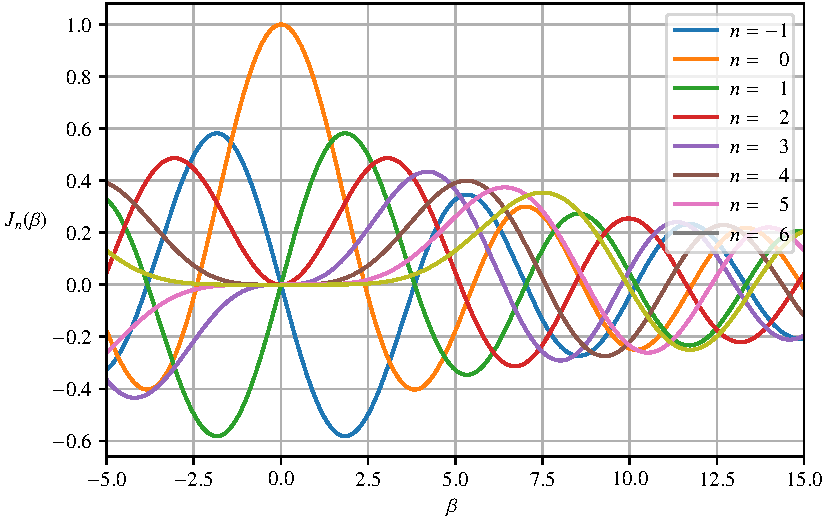
\includegraphics{papers/fm/images/bessel.pdf}
	%%% Creator: Matplotlib, PGF backend
%%
%% To include the figure in your LaTeX document, write
%%   \input{<filename>.pgf}
%%
%% Make sure the required packages are loaded in your preamble
%%   \usepackage{pgf}
%%
%% Also ensure that all the required font packages are loaded; for instance,
%% the lmodern package is sometimes necessary when using math font.
%%   \usepackage{lmodern}
%%
%% Figures using additional raster images can only be included by \input if
%% they are in the same directory as the main LaTeX file. For loading figures
%% from other directories you can use the `import` package
%%   \usepackage{import}
%%
%% and then include the figures with
%%   \import{<path to file>}{<filename>.pgf}
%%
%% Matplotlib used the following preamble
%%
\begingroup%
\makeatletter%
\begin{pgfpicture}%
\pgfpathrectangle{\pgfpointorigin}{\pgfqpoint{6.000000in}{4.000000in}}%
\pgfusepath{use as bounding box, clip}%
\begin{pgfscope}%
\pgfsetbuttcap%
\pgfsetmiterjoin%
\pgfsetlinewidth{0.000000pt}%
\definecolor{currentstroke}{rgb}{1.000000,1.000000,1.000000}%
\pgfsetstrokecolor{currentstroke}%
\pgfsetstrokeopacity{0.000000}%
\pgfsetdash{}{0pt}%
\pgfpathmoveto{\pgfqpoint{0.000000in}{0.000000in}}%
\pgfpathlineto{\pgfqpoint{6.000000in}{0.000000in}}%
\pgfpathlineto{\pgfqpoint{6.000000in}{4.000000in}}%
\pgfpathlineto{\pgfqpoint{0.000000in}{4.000000in}}%
\pgfpathlineto{\pgfqpoint{0.000000in}{0.000000in}}%
\pgfpathclose%
\pgfusepath{}%
\end{pgfscope}%
\begin{pgfscope}%
\pgfsetbuttcap%
\pgfsetmiterjoin%
\definecolor{currentfill}{rgb}{1.000000,1.000000,1.000000}%
\pgfsetfillcolor{currentfill}%
\pgfsetlinewidth{0.000000pt}%
\definecolor{currentstroke}{rgb}{0.000000,0.000000,0.000000}%
\pgfsetstrokecolor{currentstroke}%
\pgfsetstrokeopacity{0.000000}%
\pgfsetdash{}{0pt}%
\pgfpathmoveto{\pgfqpoint{0.750000in}{0.500000in}}%
\pgfpathlineto{\pgfqpoint{5.400000in}{0.500000in}}%
\pgfpathlineto{\pgfqpoint{5.400000in}{3.520000in}}%
\pgfpathlineto{\pgfqpoint{0.750000in}{3.520000in}}%
\pgfpathlineto{\pgfqpoint{0.750000in}{0.500000in}}%
\pgfpathclose%
\pgfusepath{fill}%
\end{pgfscope}%
%
\begin{pgfscope}%
\pgfpathrectangle{\pgfqpoint{0.750000in}{0.500000in}}{\pgfqpoint{4.650000in}{3.020000in}}%
\pgfusepath{clip}%
\pgfsetrectcap%
\pgfsetroundjoin%
\pgfsetlinewidth{0.803000pt}%
\definecolor{currentstroke}{rgb}{0.690196,0.690196,0.690196}%
\pgfsetstrokecolor{currentstroke}%
\pgfsetdash{}{0pt}%
\pgfpathmoveto{\pgfqpoint{0.750000in}{0.500000in}}%
\pgfpathlineto{\pgfqpoint{0.750000in}{3.520000in}}%
\pgfusepath{stroke}%
\end{pgfscope}%
%
\begin{pgfscope}%
\pgfsetbuttcap%
\pgfsetroundjoin%
\definecolor{currentfill}{rgb}{0.000000,0.000000,0.000000}%
\pgfsetfillcolor{currentfill}%
\pgfsetlinewidth{0.803000pt}%
\definecolor{currentstroke}{rgb}{0.000000,0.000000,0.000000}%
\pgfsetstrokecolor{currentstroke}%
\pgfsetdash{}{0pt}%
\pgfsys@defobject{currentmarker}{\pgfqpoint{0.000000in}{-0.048611in}}{\pgfqpoint{0.000000in}{0.000000in}}{%
\pgfpathmoveto{\pgfqpoint{0.000000in}{0.000000in}}%
\pgfpathlineto{\pgfqpoint{0.000000in}{-0.048611in}}%
\pgfusepath{stroke,fill}%
}%
%
\begin{pgfscope}%
\pgfsys@transformshift{0.750000in}{0.500000in}%
\pgfsys@useobject{currentmarker}{}%
\end{pgfscope}%
%
\end{pgfscope}%
%
\begin{pgfscope}%
\definecolor{textcolor}{rgb}{0.000000,0.000000,0.000000}%
\pgfsetstrokecolor{textcolor}%
\pgfsetfillcolor{textcolor}%
\pgftext[x=0.750000in,y=0.402778in,,top]{\color{textcolor}\rmfamily\fontsize{10.000000}{12.000000}\selectfont \(\displaystyle {\ensuremath{-}5.0}\)}%
\end{pgfscope}%
\begin{pgfscope}%
\pgfpathrectangle{\pgfqpoint{0.750000in}{0.500000in}}{\pgfqpoint{4.650000in}{3.020000in}}%
\pgfusepath{clip}%
\pgfsetrectcap%
\pgfsetroundjoin%
\pgfsetlinewidth{0.803000pt}%
\definecolor{currentstroke}{rgb}{0.690196,0.690196,0.690196}%
\pgfsetstrokecolor{currentstroke}%
\pgfsetdash{}{0pt}%
\pgfpathmoveto{\pgfqpoint{1.331250in}{0.500000in}}%
\pgfpathlineto{\pgfqpoint{1.331250in}{3.520000in}}%
\pgfusepath{stroke}%
\end{pgfscope}%
%
\begin{pgfscope}%
\pgfsetbuttcap%
\pgfsetroundjoin%
\definecolor{currentfill}{rgb}{0.000000,0.000000,0.000000}%
\pgfsetfillcolor{currentfill}%
\pgfsetlinewidth{0.803000pt}%
\definecolor{currentstroke}{rgb}{0.000000,0.000000,0.000000}%
\pgfsetstrokecolor{currentstroke}%
\pgfsetdash{}{0pt}%
\pgfsys@defobject{currentmarker}{\pgfqpoint{0.000000in}{-0.048611in}}{\pgfqpoint{0.000000in}{0.000000in}}{%
\pgfpathmoveto{\pgfqpoint{0.000000in}{0.000000in}}%
\pgfpathlineto{\pgfqpoint{0.000000in}{-0.048611in}}%
\pgfusepath{stroke,fill}%
}%
%
\begin{pgfscope}%
\pgfsys@transformshift{1.331250in}{0.500000in}%
\pgfsys@useobject{currentmarker}{}%
\end{pgfscope}%
\end{pgfscope}%
\begin{pgfscope}%
\definecolor{textcolor}{rgb}{0.000000,0.000000,0.000000}%
\pgfsetstrokecolor{textcolor}%
\pgfsetfillcolor{textcolor}%
\pgftext[x=1.331250in,y=0.402778in,,top]{\color{textcolor}\rmfamily\fontsize{10.000000}{12.000000}\selectfont \(\displaystyle {\ensuremath{-}2.5}\)}%
\end{pgfscope}%
%
\begin{pgfscope}%
\pgfpathrectangle{\pgfqpoint{0.750000in}{0.500000in}}{\pgfqpoint{4.650000in}{3.020000in}}%
\pgfusepath{clip}%
\pgfsetrectcap%
\pgfsetroundjoin%
\pgfsetlinewidth{0.803000pt}%
\definecolor{currentstroke}{rgb}{0.690196,0.690196,0.690196}%
\pgfsetstrokecolor{currentstroke}%
\pgfsetdash{}{0pt}%
\pgfpathmoveto{\pgfqpoint{1.912500in}{0.500000in}}%
\pgfpathlineto{\pgfqpoint{1.912500in}{3.520000in}}%
\pgfusepath{stroke}%
\end{pgfscope}%
%
\begin{pgfscope}%
\pgfsetbuttcap%
\pgfsetroundjoin%
\definecolor{currentfill}{rgb}{0.000000,0.000000,0.000000}%
\pgfsetfillcolor{currentfill}%
\pgfsetlinewidth{0.803000pt}%
\definecolor{currentstroke}{rgb}{0.000000,0.000000,0.000000}%
\pgfsetstrokecolor{currentstroke}%
\pgfsetdash{}{0pt}%
\pgfsys@defobject{currentmarker}{\pgfqpoint{0.000000in}{-0.048611in}}{\pgfqpoint{0.000000in}{0.000000in}}{%
\pgfpathmoveto{\pgfqpoint{0.000000in}{0.000000in}}%
\pgfpathlineto{\pgfqpoint{0.000000in}{-0.048611in}}%
\pgfusepath{stroke,fill}%
}%
\begin{pgfscope}%
\pgfsys@transformshift{1.912500in}{0.500000in}%
\pgfsys@useobject{currentmarker}{}%
\end{pgfscope}%
\end{pgfscope}%
\begin{pgfscope}%
\definecolor{textcolor}{rgb}{0.000000,0.000000,0.000000}%
\pgfsetstrokecolor{textcolor}%
\pgfsetfillcolor{textcolor}%
\pgftext[x=1.912500in,y=0.402778in,,top]{\color{textcolor}\rmfamily\fontsize{10.000000}{12.000000}\selectfont \(\displaystyle {0.0}\)}%
\end{pgfscope}%
%
\begin{pgfscope}%
\pgfpathrectangle{\pgfqpoint{0.750000in}{0.500000in}}{\pgfqpoint{4.650000in}{3.020000in}}%
\pgfusepath{clip}%
\pgfsetrectcap%
\pgfsetroundjoin%
\pgfsetlinewidth{0.803000pt}%
\definecolor{currentstroke}{rgb}{0.690196,0.690196,0.690196}%
\pgfsetstrokecolor{currentstroke}%
\pgfsetdash{}{0pt}%
\pgfpathmoveto{\pgfqpoint{2.493750in}{0.500000in}}%
\pgfpathlineto{\pgfqpoint{2.493750in}{3.520000in}}%
\pgfusepath{stroke}%
\end{pgfscope}%
\begin{pgfscope}%
\pgfsetbuttcap%
\pgfsetroundjoin%
\definecolor{currentfill}{rgb}{0.000000,0.000000,0.000000}%
\pgfsetfillcolor{currentfill}%
\pgfsetlinewidth{0.803000pt}%
\definecolor{currentstroke}{rgb}{0.000000,0.000000,0.000000}%
\pgfsetstrokecolor{currentstroke}%
\pgfsetdash{}{0pt}%
\pgfsys@defobject{currentmarker}{\pgfqpoint{0.000000in}{-0.048611in}}{\pgfqpoint{0.000000in}{0.000000in}}{%
\pgfpathmoveto{\pgfqpoint{0.000000in}{0.000000in}}%
\pgfpathlineto{\pgfqpoint{0.000000in}{-0.048611in}}%
\pgfusepath{stroke,fill}%
}%
\begin{pgfscope}%
\pgfsys@transformshift{2.493750in}{0.500000in}%
\pgfsys@useobject{currentmarker}{}%
\end{pgfscope}%
\end{pgfscope}%
\begin{pgfscope}%
\definecolor{textcolor}{rgb}{0.000000,0.000000,0.000000}%
\pgfsetstrokecolor{textcolor}%
\pgfsetfillcolor{textcolor}%
\pgftext[x=2.493750in,y=0.402778in,,top]{\color{textcolor}\rmfamily\fontsize{10.000000}{12.000000}\selectfont \(\displaystyle {2.5}\)}%
\end{pgfscope}%
\begin{pgfscope}%
\pgfpathrectangle{\pgfqpoint{0.750000in}{0.500000in}}{\pgfqpoint{4.650000in}{3.020000in}}%
\pgfusepath{clip}%
\pgfsetrectcap%
\pgfsetroundjoin%
\pgfsetlinewidth{0.803000pt}%
\definecolor{currentstroke}{rgb}{0.690196,0.690196,0.690196}%
\pgfsetstrokecolor{currentstroke}%
\pgfsetdash{}{0pt}%
\pgfpathmoveto{\pgfqpoint{3.075000in}{0.500000in}}%
\pgfpathlineto{\pgfqpoint{3.075000in}{3.520000in}}%
\pgfusepath{stroke}%
\end{pgfscope}%
\begin{pgfscope}%
\pgfsetbuttcap%
\pgfsetroundjoin%
\definecolor{currentfill}{rgb}{0.000000,0.000000,0.000000}%
\pgfsetfillcolor{currentfill}%
\pgfsetlinewidth{0.803000pt}%
\definecolor{currentstroke}{rgb}{0.000000,0.000000,0.000000}%
\pgfsetstrokecolor{currentstroke}%
\pgfsetdash{}{0pt}%
\pgfsys@defobject{currentmarker}{\pgfqpoint{0.000000in}{-0.048611in}}{\pgfqpoint{0.000000in}{0.000000in}}{%
\pgfpathmoveto{\pgfqpoint{0.000000in}{0.000000in}}%
\pgfpathlineto{\pgfqpoint{0.000000in}{-0.048611in}}%
\pgfusepath{stroke,fill}%
}%
\begin{pgfscope}%
\pgfsys@transformshift{3.075000in}{0.500000in}%
\pgfsys@useobject{currentmarker}{}%
\end{pgfscope}%
\end{pgfscope}%
\begin{pgfscope}%
\definecolor{textcolor}{rgb}{0.000000,0.000000,0.000000}%
\pgfsetstrokecolor{textcolor}%
\pgfsetfillcolor{textcolor}%
\pgftext[x=3.075000in,y=0.402778in,,top]{\color{textcolor}\rmfamily\fontsize{10.000000}{12.000000}\selectfont \(\displaystyle {5.0}\)}%
\end{pgfscope}%
\begin{pgfscope}%
\pgfpathrectangle{\pgfqpoint{0.750000in}{0.500000in}}{\pgfqpoint{4.650000in}{3.020000in}}%
\pgfusepath{clip}%
\pgfsetrectcap%
\pgfsetroundjoin%
\pgfsetlinewidth{0.803000pt}%
\definecolor{currentstroke}{rgb}{0.690196,0.690196,0.690196}%
\pgfsetstrokecolor{currentstroke}%
\pgfsetdash{}{0pt}%
\pgfpathmoveto{\pgfqpoint{3.656250in}{0.500000in}}%
\pgfpathlineto{\pgfqpoint{3.656250in}{3.520000in}}%
\pgfusepath{stroke}%
\end{pgfscope}%
\begin{pgfscope}%
\pgfsetbuttcap%
\pgfsetroundjoin%
\definecolor{currentfill}{rgb}{0.000000,0.000000,0.000000}%
\pgfsetfillcolor{currentfill}%
\pgfsetlinewidth{0.803000pt}%
\definecolor{currentstroke}{rgb}{0.000000,0.000000,0.000000}%
\pgfsetstrokecolor{currentstroke}%
\pgfsetdash{}{0pt}%
\pgfsys@defobject{currentmarker}{\pgfqpoint{0.000000in}{-0.048611in}}{\pgfqpoint{0.000000in}{0.000000in}}{%
\pgfpathmoveto{\pgfqpoint{0.000000in}{0.000000in}}%
\pgfpathlineto{\pgfqpoint{0.000000in}{-0.048611in}}%
\pgfusepath{stroke,fill}%
}%
\begin{pgfscope}%
\pgfsys@transformshift{3.656250in}{0.500000in}%
\pgfsys@useobject{currentmarker}{}%
\end{pgfscope}%
\end{pgfscope}%
\begin{pgfscope}%
\definecolor{textcolor}{rgb}{0.000000,0.000000,0.000000}%
\pgfsetstrokecolor{textcolor}%
\pgfsetfillcolor{textcolor}%
\pgftext[x=3.656250in,y=0.402778in,,top]{\color{textcolor}\rmfamily\fontsize{10.000000}{12.000000}\selectfont \(\displaystyle {7.5}\)}%
\end{pgfscope}%
\begin{pgfscope}%
\pgfpathrectangle{\pgfqpoint{0.750000in}{0.500000in}}{\pgfqpoint{4.650000in}{3.020000in}}%
\pgfusepath{clip}%
\pgfsetrectcap%
\pgfsetroundjoin%
\pgfsetlinewidth{0.803000pt}%
\definecolor{currentstroke}{rgb}{0.690196,0.690196,0.690196}%
\pgfsetstrokecolor{currentstroke}%
\pgfsetdash{}{0pt}%
\pgfpathmoveto{\pgfqpoint{4.237500in}{0.500000in}}%
\pgfpathlineto{\pgfqpoint{4.237500in}{3.520000in}}%
\pgfusepath{stroke}%
\end{pgfscope}%
\begin{pgfscope}%
\pgfsetbuttcap%
\pgfsetroundjoin%
\definecolor{currentfill}{rgb}{0.000000,0.000000,0.000000}%
\pgfsetfillcolor{currentfill}%
\pgfsetlinewidth{0.803000pt}%
\definecolor{currentstroke}{rgb}{0.000000,0.000000,0.000000}%
\pgfsetstrokecolor{currentstroke}%
\pgfsetdash{}{0pt}%
\pgfsys@defobject{currentmarker}{\pgfqpoint{0.000000in}{-0.048611in}}{\pgfqpoint{0.000000in}{0.000000in}}{%
\pgfpathmoveto{\pgfqpoint{0.000000in}{0.000000in}}%
\pgfpathlineto{\pgfqpoint{0.000000in}{-0.048611in}}%
\pgfusepath{stroke,fill}%
}%
\begin{pgfscope}%
\pgfsys@transformshift{4.237500in}{0.500000in}%
\pgfsys@useobject{currentmarker}{}%
\end{pgfscope}%
\end{pgfscope}%
\begin{pgfscope}%
\definecolor{textcolor}{rgb}{0.000000,0.000000,0.000000}%
\pgfsetstrokecolor{textcolor}%
\pgfsetfillcolor{textcolor}%
\pgftext[x=4.237500in,y=0.402778in,,top]{\color{textcolor}\rmfamily\fontsize{10.000000}{12.000000}\selectfont \(\displaystyle {10.0}\)}%
\end{pgfscope}%
\begin{pgfscope}%
\pgfpathrectangle{\pgfqpoint{0.750000in}{0.500000in}}{\pgfqpoint{4.650000in}{3.020000in}}%
\pgfusepath{clip}%
\pgfsetrectcap%
\pgfsetroundjoin%
\pgfsetlinewidth{0.803000pt}%
\definecolor{currentstroke}{rgb}{0.690196,0.690196,0.690196}%
\pgfsetstrokecolor{currentstroke}%
\pgfsetdash{}{0pt}%
\pgfpathmoveto{\pgfqpoint{4.818750in}{0.500000in}}%
\pgfpathlineto{\pgfqpoint{4.818750in}{3.520000in}}%
\pgfusepath{stroke}%
\end{pgfscope}%
\begin{pgfscope}%
\pgfsetbuttcap%
\pgfsetroundjoin%
\definecolor{currentfill}{rgb}{0.000000,0.000000,0.000000}%
\pgfsetfillcolor{currentfill}%
\pgfsetlinewidth{0.803000pt}%
\definecolor{currentstroke}{rgb}{0.000000,0.000000,0.000000}%
\pgfsetstrokecolor{currentstroke}%
\pgfsetdash{}{0pt}%
\pgfsys@defobject{currentmarker}{\pgfqpoint{0.000000in}{-0.048611in}}{\pgfqpoint{0.000000in}{0.000000in}}{%
\pgfpathmoveto{\pgfqpoint{0.000000in}{0.000000in}}%
\pgfpathlineto{\pgfqpoint{0.000000in}{-0.048611in}}%
\pgfusepath{stroke,fill}%
}%
\begin{pgfscope}%
\pgfsys@transformshift{4.818750in}{0.500000in}%
\pgfsys@useobject{currentmarker}{}%
\end{pgfscope}%
\end{pgfscope}%
\begin{pgfscope}%
\definecolor{textcolor}{rgb}{0.000000,0.000000,0.000000}%
\pgfsetstrokecolor{textcolor}%
\pgfsetfillcolor{textcolor}%
\pgftext[x=4.818750in,y=0.402778in,,top]{\color{textcolor}\rmfamily\fontsize{10.000000}{12.000000}\selectfont \(\displaystyle {12.5}\)}%
\end{pgfscope}%
\begin{pgfscope}%
\pgfpathrectangle{\pgfqpoint{0.750000in}{0.500000in}}{\pgfqpoint{4.650000in}{3.020000in}}%
\pgfusepath{clip}%
\pgfsetrectcap%
\pgfsetroundjoin%
\pgfsetlinewidth{0.803000pt}%
\definecolor{currentstroke}{rgb}{0.690196,0.690196,0.690196}%
\pgfsetstrokecolor{currentstroke}%
\pgfsetdash{}{0pt}%
\pgfpathmoveto{\pgfqpoint{5.400000in}{0.500000in}}%
\pgfpathlineto{\pgfqpoint{5.400000in}{3.520000in}}%
\pgfusepath{stroke}%
\end{pgfscope}%
\begin{pgfscope}%
\pgfsetbuttcap%
\pgfsetroundjoin%
\definecolor{currentfill}{rgb}{0.000000,0.000000,0.000000}%
\pgfsetfillcolor{currentfill}%
\pgfsetlinewidth{0.803000pt}%
\definecolor{currentstroke}{rgb}{0.000000,0.000000,0.000000}%
\pgfsetstrokecolor{currentstroke}%
\pgfsetdash{}{0pt}%
\pgfsys@defobject{currentmarker}{\pgfqpoint{0.000000in}{-0.048611in}}{\pgfqpoint{0.000000in}{0.000000in}}{%
\pgfpathmoveto{\pgfqpoint{0.000000in}{0.000000in}}%
\pgfpathlineto{\pgfqpoint{0.000000in}{-0.048611in}}%
\pgfusepath{stroke,fill}%
}%
\begin{pgfscope}%
\pgfsys@transformshift{5.400000in}{0.500000in}%
\pgfsys@useobject{currentmarker}{}%
\end{pgfscope}%
\end{pgfscope}%
\begin{pgfscope}%
\definecolor{textcolor}{rgb}{0.000000,0.000000,0.000000}%
\pgfsetstrokecolor{textcolor}%
\pgfsetfillcolor{textcolor}%
\pgftext[x=5.400000in,y=0.402778in,,top]{\color{textcolor}\rmfamily\fontsize{10.000000}{12.000000}\selectfont \(\displaystyle {15.0}\)}%
\end{pgfscope}%
\begin{pgfscope}%
\definecolor{textcolor}{rgb}{0.000000,0.000000,0.000000}%
\pgfsetstrokecolor{textcolor}%
\pgfsetfillcolor{textcolor}%
\pgftext[x=3.075000in,y=0.223766in,,top]{\color{textcolor}\rmfamily\fontsize{10.000000}{12.000000}\selectfont  \(\displaystyle  \beta \) }%
\end{pgfscope}%
\begin{pgfscope}%
\pgfpathrectangle{\pgfqpoint{0.750000in}{0.500000in}}{\pgfqpoint{4.650000in}{3.020000in}}%
\pgfusepath{clip}%
\pgfsetrectcap%
\pgfsetroundjoin%
\pgfsetlinewidth{0.803000pt}%
\definecolor{currentstroke}{rgb}{0.690196,0.690196,0.690196}%
\pgfsetstrokecolor{currentstroke}%
\pgfsetdash{}{0pt}%
\pgfpathmoveto{\pgfqpoint{0.750000in}{0.605798in}}%
\pgfpathlineto{\pgfqpoint{5.400000in}{0.605798in}}%
\pgfusepath{stroke}%
\end{pgfscope}%
\begin{pgfscope}%
\pgfsetbuttcap%
\pgfsetroundjoin%
\definecolor{currentfill}{rgb}{0.000000,0.000000,0.000000}%
\pgfsetfillcolor{currentfill}%
\pgfsetlinewidth{0.803000pt}%
\definecolor{currentstroke}{rgb}{0.000000,0.000000,0.000000}%
\pgfsetstrokecolor{currentstroke}%
\pgfsetdash{}{0pt}%
\pgfsys@defobject{currentmarker}{\pgfqpoint{-0.048611in}{0.000000in}}{\pgfqpoint{-0.000000in}{0.000000in}}{%
\pgfpathmoveto{\pgfqpoint{-0.000000in}{0.000000in}}%
\pgfpathlineto{\pgfqpoint{-0.048611in}{0.000000in}}%
\pgfusepath{stroke,fill}%
}%
\begin{pgfscope}%
\pgfsys@transformshift{0.750000in}{0.605798in}%
\pgfsys@useobject{currentmarker}{}%
\end{pgfscope}%
\end{pgfscope}%
\begin{pgfscope}%
\definecolor{textcolor}{rgb}{0.000000,0.000000,0.000000}%
\pgfsetstrokecolor{textcolor}%
\pgfsetfillcolor{textcolor}%
\pgftext[x=0.65in, y=0.557573in, right, base]{\color{textcolor}\rmfamily\fontsize{10.000000}{12.000000}\selectfont \(\displaystyle {\ensuremath{-}0.6}\)}%
\end{pgfscope}%
\begin{pgfscope}%
\pgfpathrectangle{\pgfqpoint{0.750000in}{0.500000in}}{\pgfqpoint{4.650000in}{3.020000in}}%
\pgfusepath{clip}%
\pgfsetrectcap%
\pgfsetroundjoin%
\pgfsetlinewidth{0.803000pt}%
\definecolor{currentstroke}{rgb}{0.690196,0.690196,0.690196}%
\pgfsetstrokecolor{currentstroke}%
\pgfsetdash{}{0pt}%
\pgfpathmoveto{\pgfqpoint{0.750000in}{0.952915in}}%
\pgfpathlineto{\pgfqpoint{5.400000in}{0.952915in}}%
\pgfusepath{stroke}%
\end{pgfscope}%
\begin{pgfscope}%
\pgfsetbuttcap%
\pgfsetroundjoin%
\definecolor{currentfill}{rgb}{0.000000,0.000000,0.000000}%
\pgfsetfillcolor{currentfill}%
\pgfsetlinewidth{0.803000pt}%
\definecolor{currentstroke}{rgb}{0.000000,0.000000,0.000000}%
\pgfsetstrokecolor{currentstroke}%
\pgfsetdash{}{0pt}%
\pgfsys@defobject{currentmarker}{\pgfqpoint{-0.048611in}{0.000000in}}{\pgfqpoint{-0.000000in}{0.000000in}}{%
\pgfpathmoveto{\pgfqpoint{-0.000000in}{0.000000in}}%
\pgfpathlineto{\pgfqpoint{-0.048611in}{0.000000in}}%
\pgfusepath{stroke,fill}%
}%
\begin{pgfscope}%
\pgfsys@transformshift{0.750000in}{0.952915in}%
\pgfsys@useobject{currentmarker}{}%
\end{pgfscope}%
\end{pgfscope}%
\begin{pgfscope}%
\definecolor{textcolor}{rgb}{0.000000,0.000000,0.000000}%
\pgfsetstrokecolor{textcolor}%
\pgfsetfillcolor{textcolor}%
\pgftext[x=0.65in, y=0.904689in, right, base]{\color{textcolor}\rmfamily\fontsize{10.000000}{12.000000}\selectfont \(\displaystyle {\ensuremath{-0.4}}\)}%
\end{pgfscope}%
\begin{pgfscope}%
\pgfpathrectangle{\pgfqpoint{0.750000in}{0.500000in}}{\pgfqpoint{4.650000in}{3.020000in}}%
\pgfusepath{clip}%
\pgfsetrectcap%
\pgfsetroundjoin%
\pgfsetlinewidth{0.803000pt}%
\definecolor{currentstroke}{rgb}{0.690196,0.690196,0.690196}%
\pgfsetstrokecolor{currentstroke}%
\pgfsetdash{}{0pt}%
\pgfpathmoveto{\pgfqpoint{0.750000in}{1.300031in}}%
\pgfpathlineto{\pgfqpoint{5.400000in}{1.300031in}}%
\pgfusepath{stroke}%
\end{pgfscope}%
\begin{pgfscope}%
\pgfsetbuttcap%
\pgfsetroundjoin%
\definecolor{currentfill}{rgb}{0.000000,0.000000,0.000000}%
\pgfsetfillcolor{currentfill}%
\pgfsetlinewidth{0.803000pt}%
\definecolor{currentstroke}{rgb}{0.000000,0.000000,0.000000}%
\pgfsetstrokecolor{currentstroke}%
\pgfsetdash{}{0pt}%
\pgfsys@defobject{currentmarker}{\pgfqpoint{-0.048611in}{0.000000in}}{\pgfqpoint{-0.000000in}{0.000000in}}{%
\pgfpathmoveto{\pgfqpoint{-0.000000in}{0.000000in}}%
\pgfpathlineto{\pgfqpoint{-0.048611in}{0.000000in}}%
\pgfusepath{stroke,fill}%
}%
\begin{pgfscope}%
\pgfsys@transformshift{0.750000in}{1.300031in}%
\pgfsys@useobject{currentmarker}{}%
\end{pgfscope}%
\end{pgfscope}%
\begin{pgfscope}%
\definecolor{textcolor}{rgb}{0.000000,0.000000,0.000000}%
\pgfsetstrokecolor{textcolor}%
\pgfsetfillcolor{textcolor}%
\pgftext[x=0.65in, y=1.251806in, right, base]{\color{textcolor}\rmfamily\fontsize{10.000000}{12.000000}\selectfont \(\displaystyle {\ensuremath{-0.2}}\)}%
\end{pgfscope}%
\begin{pgfscope}%
\pgfpathrectangle{\pgfqpoint{0.750000in}{0.500000in}}{\pgfqpoint{4.650000in}{3.020000in}}%
\pgfusepath{clip}%
\pgfsetrectcap%
\pgfsetroundjoin%
\pgfsetlinewidth{0.803000pt}%
\definecolor{currentstroke}{rgb}{0.690196,0.690196,0.690196}%
\pgfsetstrokecolor{currentstroke}%
\pgfsetdash{}{0pt}%
\pgfpathmoveto{\pgfqpoint{0.750000in}{1.647147in}}%
\pgfpathlineto{\pgfqpoint{5.400000in}{1.647147in}}%
\pgfusepath{stroke}%
\end{pgfscope}%
\begin{pgfscope}%
\pgfsetbuttcap%
\pgfsetroundjoin%
\definecolor{currentfill}{rgb}{0.000000,0.000000,0.000000}%
\pgfsetfillcolor{currentfill}%
\pgfsetlinewidth{0.803000pt}%
\definecolor{currentstroke}{rgb}{0.000000,0.000000,0.000000}%
\pgfsetstrokecolor{currentstroke}%
\pgfsetdash{}{0pt}%
\pgfsys@defobject{currentmarker}{\pgfqpoint{-0.048611in}{0.000000in}}{\pgfqpoint{-0.000000in}{0.000000in}}{%
\pgfpathmoveto{\pgfqpoint{-0.000000in}{0.000000in}}%
\pgfpathlineto{\pgfqpoint{-0.048611in}{0.000000in}}%
\pgfusepath{stroke,fill}%
}%
\begin{pgfscope}%
\pgfsys@transformshift{0.750000in}{1.647147in}%
\pgfsys@useobject{currentmarker}{}%
\end{pgfscope}%
\end{pgfscope}%
\begin{pgfscope}%
\definecolor{textcolor}{rgb}{0.000000,0.000000,0.000000}%
\pgfsetstrokecolor{textcolor}%
\pgfsetfillcolor{textcolor}%
\pgftext[x=0.65in, y=1.598922in, right, base]{\color{textcolor}\rmfamily\fontsize{10.000000}{12.000000}\selectfont \(\displaystyle 0.0\)}%
\end{pgfscope}%
\begin{pgfscope}%
\pgfpathrectangle{\pgfqpoint{0.750000in}{0.500000in}}{\pgfqpoint{4.650000in}{3.020000in}}%
\pgfusepath{clip}%
\pgfsetrectcap%
\pgfsetroundjoin%
\pgfsetlinewidth{0.803000pt}%
\definecolor{currentstroke}{rgb}{0.690196,0.690196,0.690196}%
\pgfsetstrokecolor{currentstroke}%
\pgfsetdash{}{0pt}%
\pgfpathmoveto{\pgfqpoint{0.750000in}{1.994263in}}%
\pgfpathlineto{\pgfqpoint{5.400000in}{1.994263in}}%
\pgfusepath{stroke}%
\end{pgfscope}%
\begin{pgfscope}%
\pgfsetbuttcap%
\pgfsetroundjoin%
\definecolor{currentfill}{rgb}{0.000000,0.000000,0.000000}%
\pgfsetfillcolor{currentfill}%
\pgfsetlinewidth{0.803000pt}%
\definecolor{currentstroke}{rgb}{0.000000,0.000000,0.000000}%
\pgfsetstrokecolor{currentstroke}%
\pgfsetdash{}{0pt}%
\pgfsys@defobject{currentmarker}{\pgfqpoint{-0.048611in}{0.000000in}}{\pgfqpoint{-0.000000in}{0.000000in}}{%
\pgfpathmoveto{\pgfqpoint{-0.000000in}{0.000000in}}%
\pgfpathlineto{\pgfqpoint{-0.048611in}{0.000000in}}%
\pgfusepath{stroke,fill}%
}%
\begin{pgfscope}%
\pgfsys@transformshift{0.750000in}{1.994263in}%
\pgfsys@useobject{currentmarker}{}%
\end{pgfscope}%
\end{pgfscope}%
\begin{pgfscope}%
\definecolor{textcolor}{rgb}{0.000000,0.000000,0.000000}%
\pgfsetstrokecolor{textcolor}%
\pgfsetfillcolor{textcolor}%
\pgftext[x=0.65in, y=1.946038in, right, base]{\color{textcolor}\rmfamily\fontsize{10.000000}{12.000000}\selectfont \(\displaystyle {0.2}\)}%
\end{pgfscope}%
\begin{pgfscope}%
\pgfpathrectangle{\pgfqpoint{0.750000in}{0.500000in}}{\pgfqpoint{4.650000in}{3.020000in}}%
\pgfusepath{clip}%
\pgfsetrectcap%
\pgfsetroundjoin%
\pgfsetlinewidth{0.803000pt}%
\definecolor{currentstroke}{rgb}{0.690196,0.690196,0.690196}%
\pgfsetstrokecolor{currentstroke}%
\pgfsetdash{}{0pt}%
\pgfpathmoveto{\pgfqpoint{0.750000in}{2.341380in}}%
\pgfpathlineto{\pgfqpoint{5.400000in}{2.341380in}}%
\pgfusepath{stroke}%
\end{pgfscope}%
\begin{pgfscope}%
\pgfsetbuttcap%
\pgfsetroundjoin%
\definecolor{currentfill}{rgb}{0.000000,0.000000,0.000000}%
\pgfsetfillcolor{currentfill}%
\pgfsetlinewidth{0.803000pt}%
\definecolor{currentstroke}{rgb}{0.000000,0.000000,0.000000}%
\pgfsetstrokecolor{currentstroke}%
\pgfsetdash{}{0pt}%
\pgfsys@defobject{currentmarker}{\pgfqpoint{-0.048611in}{0.000000in}}{\pgfqpoint{-0.000000in}{0.000000in}}{%
\pgfpathmoveto{\pgfqpoint{-0.000000in}{0.000000in}}%
\pgfpathlineto{\pgfqpoint{-0.048611in}{0.000000in}}%
\pgfusepath{stroke,fill}%
}%
\begin{pgfscope}%
\pgfsys@transformshift{0.750000in}{2.341380in}%
\pgfsys@useobject{currentmarker}{}%
\end{pgfscope}%
\end{pgfscope}%
\begin{pgfscope}%
\definecolor{textcolor}{rgb}{0.000000,0.000000,0.000000}%
\pgfsetstrokecolor{textcolor}%
\pgfsetfillcolor{textcolor}%
\pgftext[x=0.65in, y=2.293154in, right, base]{\color{textcolor}\rmfamily\fontsize{10.000000}{12.000000}\selectfont \(\displaystyle {0.4}\)}%
\end{pgfscope}%
\begin{pgfscope}%
\pgfpathrectangle{\pgfqpoint{0.750000in}{0.500000in}}{\pgfqpoint{4.650000in}{3.020000in}}%
\pgfusepath{clip}%
\pgfsetrectcap%
\pgfsetroundjoin%
\pgfsetlinewidth{0.803000pt}%
\definecolor{currentstroke}{rgb}{0.690196,0.690196,0.690196}%
\pgfsetstrokecolor{currentstroke}%
\pgfsetdash{}{0pt}%
\pgfpathmoveto{\pgfqpoint{0.750000in}{2.688496in}}%
\pgfpathlineto{\pgfqpoint{5.400000in}{2.688496in}}%
\pgfusepath{stroke}%
\end{pgfscope}%
\begin{pgfscope}%
\pgfsetbuttcap%
\pgfsetroundjoin%
\definecolor{currentfill}{rgb}{0.000000,0.000000,0.000000}%
\pgfsetfillcolor{currentfill}%
\pgfsetlinewidth{0.803000pt}%
\definecolor{currentstroke}{rgb}{0.000000,0.000000,0.000000}%
\pgfsetstrokecolor{currentstroke}%
\pgfsetdash{}{0pt}%
\pgfsys@defobject{currentmarker}{\pgfqpoint{-0.048611in}{0.000000in}}{\pgfqpoint{-0.000000in}{0.000000in}}{%
\pgfpathmoveto{\pgfqpoint{-0.000000in}{0.000000in}}%
\pgfpathlineto{\pgfqpoint{-0.048611in}{0.000000in}}%
\pgfusepath{stroke,fill}%
}%
\begin{pgfscope}%
\pgfsys@transformshift{0.750000in}{2.688496in}%
\pgfsys@useobject{currentmarker}{}%
\end{pgfscope}%
\end{pgfscope}%
\begin{pgfscope}%
\definecolor{textcolor}{rgb}{0.000000,0.000000,0.000000}%
\pgfsetstrokecolor{textcolor}%
\pgfsetfillcolor{textcolor}%
\pgftext[x=0.65in, y=2.640271in, right, base]{\color{textcolor}\rmfamily\fontsize{10.000000}{12.000000}\selectfont \(\displaystyle {0.6}\)}%
\end{pgfscope}%
\begin{pgfscope}%
\pgfpathrectangle{\pgfqpoint{0.750000in}{0.500000in}}{\pgfqpoint{4.650000in}{3.020000in}}%
\pgfusepath{clip}%
\pgfsetrectcap%
\pgfsetroundjoin%
\pgfsetlinewidth{0.803000pt}%
\definecolor{currentstroke}{rgb}{0.690196,0.690196,0.690196}%
\pgfsetstrokecolor{currentstroke}%
\pgfsetdash{}{0pt}%
\pgfpathmoveto{\pgfqpoint{0.750000in}{3.035612in}}%
\pgfpathlineto{\pgfqpoint{5.400000in}{3.035612in}}%
\pgfusepath{stroke}%
\end{pgfscope}%
\begin{pgfscope}%
\pgfsetbuttcap%
\pgfsetroundjoin%
\definecolor{currentfill}{rgb}{0.000000,0.000000,0.000000}%
\pgfsetfillcolor{currentfill}%
\pgfsetlinewidth{0.803000pt}%
\definecolor{currentstroke}{rgb}{0.000000,0.000000,0.000000}%
\pgfsetstrokecolor{currentstroke}%
\pgfsetdash{}{0pt}%
\pgfsys@defobject{currentmarker}{\pgfqpoint{-0.048611in}{0.000000in}}{\pgfqpoint{-0.000000in}{0.000000in}}{%
\pgfpathmoveto{\pgfqpoint{-0.000000in}{0.000000in}}%
\pgfpathlineto{\pgfqpoint{-0.048611in}{0.000000in}}%
\pgfusepath{stroke,fill}%
}%
\begin{pgfscope}%
\pgfsys@transformshift{0.750000in}{3.035612in}%
\pgfsys@useobject{currentmarker}{}%
\end{pgfscope}%
\end{pgfscope}%
\begin{pgfscope}%
\definecolor{textcolor}{rgb}{0.000000,0.000000,0.000000}%
\pgfsetstrokecolor{textcolor}%
\pgfsetfillcolor{textcolor}%
\pgftext[x=0.65in, y=2.987387in, right, base]{\color{textcolor}\rmfamily\fontsize{10.000000}{12.000000}\selectfont \(\displaystyle {0.8}\)}%
\end{pgfscope}%
\begin{pgfscope}%
\pgfpathrectangle{\pgfqpoint{0.750000in}{0.500000in}}{\pgfqpoint{4.650000in}{3.020000in}}%
\pgfusepath{clip}%
\pgfsetrectcap%
\pgfsetroundjoin%
\pgfsetlinewidth{0.803000pt}%
\definecolor{currentstroke}{rgb}{0.690196,0.690196,0.690196}%
\pgfsetstrokecolor{currentstroke}%
\pgfsetdash{}{0pt}%
\pgfpathmoveto{\pgfqpoint{0.750000in}{3.382728in}}%
\pgfpathlineto{\pgfqpoint{5.400000in}{3.382728in}}%
\pgfusepath{stroke}%
\end{pgfscope}%
\begin{pgfscope}%
\pgfsetbuttcap%
\pgfsetroundjoin%
\definecolor{currentfill}{rgb}{0.000000,0.000000,0.000000}%
\pgfsetfillcolor{currentfill}%
\pgfsetlinewidth{0.803000pt}%
\definecolor{currentstroke}{rgb}{0.000000,0.000000,0.000000}%
\pgfsetstrokecolor{currentstroke}%
\pgfsetdash{}{0pt}%
\pgfsys@defobject{currentmarker}{\pgfqpoint{-0.048611in}{0.000000in}}{\pgfqpoint{-0.000000in}{0.000000in}}{%
\pgfpathmoveto{\pgfqpoint{-0.000000in}{0.000000in}}%
\pgfpathlineto{\pgfqpoint{-0.048611in}{0.000000in}}%
\pgfusepath{stroke,fill}%
}%
\begin{pgfscope}%
\pgfsys@transformshift{0.750000in}{3.382728in}%
\pgfsys@useobject{currentmarker}{}%
\end{pgfscope}%
\end{pgfscope}%
\begin{pgfscope}%
\definecolor{textcolor}{rgb}{0.000000,0.000000,0.000000}%
\pgfsetstrokecolor{textcolor}%
\pgfsetfillcolor{textcolor}%
\pgftext[x=0.65in, y=3.334503in, right, base]{\color{textcolor}\rmfamily\fontsize{10.000000}{12.000000}\selectfont \(\displaystyle {1.0}\)}%
\end{pgfscope}%
\begin{pgfscope}%
\definecolor{textcolor}{rgb}{0.000000,0.000000,0.000000}%
\pgfsetstrokecolor{textcolor}%
\pgfsetfillcolor{textcolor}%
\pgftext[x=0.211727in,y=2.010000in,,bottom,rotate=00.000000]{\color{textcolor}\rmfamily\fontsize{10.000000}{12.000000}\selectfont \(\displaystyle J_n(\beta)\)}%
\end{pgfscope}%
%
\begin{pgfscope}%
\pgfpathrectangle{\pgfqpoint{0.750000in}{0.500000in}}{\pgfqpoint{4.650000in}{3.020000in}}%
\pgfusepath{clip}%
\pgfsetrectcap%
\pgfsetroundjoin%
\pgfsetlinewidth{1.505625pt}%
\definecolor{currentstroke}{rgb}{0.121569,0.466667,0.705882}%
\pgfsetstrokecolor{currentstroke}%
\pgfsetdash{}{0pt}%
\pgfpathmoveto{\pgfqpoint{0.749767in}{1.078413in}}%
\pgfpathlineto{\pgfqpoint{0.769208in}{1.096666in}}%
\pgfpathlineto{\pgfqpoint{0.789672in}{1.120234in}}%
\pgfpathlineto{\pgfqpoint{0.811160in}{1.149687in}}%
\pgfpathlineto{\pgfqpoint{0.834693in}{1.187305in}}%
\pgfpathlineto{\pgfqpoint{0.860274in}{1.234274in}}%
\pgfpathlineto{\pgfqpoint{0.887900in}{1.291687in}}%
\pgfpathlineto{\pgfqpoint{0.918596in}{1.362946in}}%
\pgfpathlineto{\pgfqpoint{0.952362in}{1.449362in}}%
\pgfpathlineto{\pgfqpoint{0.991244in}{1.557556in}}%
\pgfpathlineto{\pgfqpoint{1.040358in}{1.704000in}}%
\pgfpathlineto{\pgfqpoint{1.220442in}{2.250681in}}%
\pgfpathlineto{\pgfqpoint{1.257277in}{2.347717in}}%
\pgfpathlineto{\pgfqpoint{1.290020in}{2.425499in}}%
\pgfpathlineto{\pgfqpoint{1.318669in}{2.485878in}}%
\pgfpathlineto{\pgfqpoint{1.344249in}{2.533008in}}%
\pgfpathlineto{\pgfqpoint{1.367783in}{2.570238in}}%
\pgfpathlineto{\pgfqpoint{1.389270in}{2.598777in}}%
\pgfpathlineto{\pgfqpoint{1.409734in}{2.620884in}}%
\pgfpathlineto{\pgfqpoint{1.428152in}{2.636398in}}%
\pgfpathlineto{\pgfqpoint{1.445547in}{2.647135in}}%
\pgfpathlineto{\pgfqpoint{1.461918in}{2.653697in}}%
\pgfpathlineto{\pgfqpoint{1.477266in}{2.656684in}}%
\pgfpathlineto{\pgfqpoint{1.492614in}{2.656579in}}%
\pgfpathlineto{\pgfqpoint{1.507962in}{2.653365in}}%
\pgfpathlineto{\pgfqpoint{1.523310in}{2.647033in}}%
\pgfpathlineto{\pgfqpoint{1.539681in}{2.636850in}}%
\pgfpathlineto{\pgfqpoint{1.557076in}{2.622171in}}%
\pgfpathlineto{\pgfqpoint{1.575494in}{2.602340in}}%
\pgfpathlineto{\pgfqpoint{1.594934in}{2.576698in}}%
\pgfpathlineto{\pgfqpoint{1.615399in}{2.544600in}}%
\pgfpathlineto{\pgfqpoint{1.637909in}{2.503432in}}%
\pgfpathlineto{\pgfqpoint{1.662466in}{2.451816in}}%
\pgfpathlineto{\pgfqpoint{1.689069in}{2.388452in}}%
\pgfpathlineto{\pgfqpoint{1.718742in}{2.309344in}}%
\pgfpathlineto{\pgfqpoint{1.751485in}{2.212809in}}%
\pgfpathlineto{\pgfqpoint{1.788320in}{2.094308in}}%
\pgfpathlineto{\pgfqpoint{1.832318in}{1.941994in}}%
\pgfpathlineto{\pgfqpoint{1.893710in}{1.717221in}}%
\pgfpathlineto{\pgfqpoint{2.005240in}{1.307842in}}%
\pgfpathlineto{\pgfqpoint{2.050261in}{1.155202in}}%
\pgfpathlineto{\pgfqpoint{2.088119in}{1.037311in}}%
\pgfpathlineto{\pgfqpoint{2.120862in}{0.944956in}}%
\pgfpathlineto{\pgfqpoint{2.150535in}{0.870131in}}%
\pgfpathlineto{\pgfqpoint{2.177138in}{0.810959in}}%
\pgfpathlineto{\pgfqpoint{2.201695in}{0.763466in}}%
\pgfpathlineto{\pgfqpoint{2.224205in}{0.726259in}}%
\pgfpathlineto{\pgfqpoint{2.245693in}{0.696606in}}%
\pgfpathlineto{\pgfqpoint{2.265134in}{0.674846in}}%
\pgfpathlineto{\pgfqpoint{2.283551in}{0.658755in}}%
\pgfpathlineto{\pgfqpoint{2.300946in}{0.647647in}}%
\pgfpathlineto{\pgfqpoint{2.317317in}{0.640843in}}%
\pgfpathlineto{\pgfqpoint{2.332665in}{0.637685in}}%
\pgfpathlineto{\pgfqpoint{2.348013in}{0.637637in}}%
\pgfpathlineto{\pgfqpoint{2.363361in}{0.640680in}}%
\pgfpathlineto{\pgfqpoint{2.378709in}{0.646786in}}%
\pgfpathlineto{\pgfqpoint{2.395081in}{0.656630in}}%
\pgfpathlineto{\pgfqpoint{2.412475in}{0.670789in}}%
\pgfpathlineto{\pgfqpoint{2.430893in}{0.689838in}}%
\pgfpathlineto{\pgfqpoint{2.451357in}{0.715745in}}%
\pgfpathlineto{\pgfqpoint{2.472844in}{0.748102in}}%
\pgfpathlineto{\pgfqpoint{2.496378in}{0.789285in}}%
\pgfpathlineto{\pgfqpoint{2.521958in}{0.840404in}}%
\pgfpathlineto{\pgfqpoint{2.550608in}{0.904826in}}%
\pgfpathlineto{\pgfqpoint{2.582327in}{0.983948in}}%
\pgfpathlineto{\pgfqpoint{2.619162in}{1.084432in}}%
\pgfpathlineto{\pgfqpoint{2.664183in}{1.216714in}}%
\pgfpathlineto{\pgfqpoint{2.733761in}{1.432234in}}%
\pgfpathlineto{\pgfqpoint{2.816641in}{1.686727in}}%
\pgfpathlineto{\pgfqpoint{2.862685in}{1.818042in}}%
\pgfpathlineto{\pgfqpoint{2.900544in}{1.916920in}}%
\pgfpathlineto{\pgfqpoint{2.933286in}{1.994166in}}%
\pgfpathlineto{\pgfqpoint{2.962959in}{2.056550in}}%
\pgfpathlineto{\pgfqpoint{2.989562in}{2.105711in}}%
\pgfpathlineto{\pgfqpoint{3.014119in}{2.145020in}}%
\pgfpathlineto{\pgfqpoint{3.037653in}{2.176960in}}%
\pgfpathlineto{\pgfqpoint{3.059140in}{2.201062in}}%
\pgfpathlineto{\pgfqpoint{3.079604in}{2.219425in}}%
\pgfpathlineto{\pgfqpoint{3.099045in}{2.232668in}}%
\pgfpathlineto{\pgfqpoint{3.117463in}{2.241415in}}%
\pgfpathlineto{\pgfqpoint{3.134857in}{2.246285in}}%
\pgfpathlineto{\pgfqpoint{3.152252in}{2.247877in}}%
\pgfpathlineto{\pgfqpoint{3.169646in}{2.246227in}}%
\pgfpathlineto{\pgfqpoint{3.187041in}{2.241385in}}%
\pgfpathlineto{\pgfqpoint{3.205459in}{2.232852in}}%
\pgfpathlineto{\pgfqpoint{3.223876in}{2.220910in}}%
\pgfpathlineto{\pgfqpoint{3.244340in}{2.203783in}}%
\pgfpathlineto{\pgfqpoint{3.265828in}{2.181621in}}%
\pgfpathlineto{\pgfqpoint{3.289361in}{2.152718in}}%
\pgfpathlineto{\pgfqpoint{3.314941in}{2.116217in}}%
\pgfpathlineto{\pgfqpoint{3.343591in}{2.069653in}}%
\pgfpathlineto{\pgfqpoint{3.375311in}{2.012008in}}%
\pgfpathlineto{\pgfqpoint{3.412146in}{1.938491in}}%
\pgfpathlineto{\pgfqpoint{3.459213in}{1.837175in}}%
\pgfpathlineto{\pgfqpoint{3.628042in}{1.466702in}}%
\pgfpathlineto{\pgfqpoint{3.665901in}{1.394777in}}%
\pgfpathlineto{\pgfqpoint{3.698643in}{1.338988in}}%
\pgfpathlineto{\pgfqpoint{3.728316in}{1.294417in}}%
\pgfpathlineto{\pgfqpoint{3.754919in}{1.259815in}}%
\pgfpathlineto{\pgfqpoint{3.779476in}{1.232700in}}%
\pgfpathlineto{\pgfqpoint{3.803010in}{1.211285in}}%
\pgfpathlineto{\pgfqpoint{3.824497in}{1.195774in}}%
\pgfpathlineto{\pgfqpoint{3.844961in}{1.184672in}}%
\pgfpathlineto{\pgfqpoint{3.864402in}{1.177483in}}%
\pgfpathlineto{\pgfqpoint{3.883843in}{1.173586in}}%
\pgfpathlineto{\pgfqpoint{3.902261in}{1.172924in}}%
\pgfpathlineto{\pgfqpoint{3.921702in}{1.175399in}}%
\pgfpathlineto{\pgfqpoint{3.941143in}{1.181088in}}%
\pgfpathlineto{\pgfqpoint{3.961607in}{1.190471in}}%
\pgfpathlineto{\pgfqpoint{3.983094in}{1.203958in}}%
\pgfpathlineto{\pgfqpoint{4.005605in}{1.221921in}}%
\pgfpathlineto{\pgfqpoint{4.029138in}{1.244674in}}%
\pgfpathlineto{\pgfqpoint{4.054718in}{1.273703in}}%
\pgfpathlineto{\pgfqpoint{4.083368in}{1.311052in}}%
\pgfpathlineto{\pgfqpoint{4.115088in}{1.357642in}}%
\pgfpathlineto{\pgfqpoint{4.151923in}{1.417475in}}%
\pgfpathlineto{\pgfqpoint{4.196944in}{1.496779in}}%
\pgfpathlineto{\pgfqpoint{4.274707in}{1.641320in}}%
\pgfpathlineto{\pgfqpoint{4.342239in}{1.764103in}}%
\pgfpathlineto{\pgfqpoint{4.385214in}{1.836076in}}%
\pgfpathlineto{\pgfqpoint{4.421026in}{1.890363in}}%
\pgfpathlineto{\pgfqpoint{4.452745in}{1.933103in}}%
\pgfpathlineto{\pgfqpoint{4.481395in}{1.966767in}}%
\pgfpathlineto{\pgfqpoint{4.507998in}{1.993420in}}%
\pgfpathlineto{\pgfqpoint{4.532555in}{2.013820in}}%
\pgfpathlineto{\pgfqpoint{4.556089in}{2.029407in}}%
\pgfpathlineto{\pgfqpoint{4.578599in}{2.040571in}}%
\pgfpathlineto{\pgfqpoint{4.600087in}{2.047743in}}%
\pgfpathlineto{\pgfqpoint{4.620551in}{2.051378in}}%
\pgfpathlineto{\pgfqpoint{4.641015in}{2.051891in}}%
\pgfpathlineto{\pgfqpoint{4.661479in}{2.049301in}}%
\pgfpathlineto{\pgfqpoint{4.681943in}{2.043650in}}%
\pgfpathlineto{\pgfqpoint{4.703430in}{2.034494in}}%
\pgfpathlineto{\pgfqpoint{4.725941in}{2.021472in}}%
\pgfpathlineto{\pgfqpoint{4.749474in}{2.004264in}}%
\pgfpathlineto{\pgfqpoint{4.775055in}{1.981626in}}%
\pgfpathlineto{\pgfqpoint{4.802681in}{1.952920in}}%
\pgfpathlineto{\pgfqpoint{4.833377in}{1.916366in}}%
\pgfpathlineto{\pgfqpoint{4.868166in}{1.869838in}}%
\pgfpathlineto{\pgfqpoint{4.909094in}{1.809589in}}%
\pgfpathlineto{\pgfqpoint{4.963324in}{1.723717in}}%
\pgfpathlineto{\pgfqpoint{5.088155in}{1.524064in}}%
\pgfpathlineto{\pgfqpoint{5.130107in}{1.463808in}}%
\pgfpathlineto{\pgfqpoint{5.165919in}{1.417576in}}%
\pgfpathlineto{\pgfqpoint{5.197638in}{1.381514in}}%
\pgfpathlineto{\pgfqpoint{5.226288in}{1.353425in}}%
\pgfpathlineto{\pgfqpoint{5.252891in}{1.331504in}}%
\pgfpathlineto{\pgfqpoint{5.277448in}{1.315051in}}%
\pgfpathlineto{\pgfqpoint{5.300982in}{1.302838in}}%
\pgfpathlineto{\pgfqpoint{5.323492in}{1.294505in}}%
\pgfpathlineto{\pgfqpoint{5.346003in}{1.289505in}}%
\pgfpathlineto{\pgfqpoint{5.367490in}{1.287862in}}%
\pgfpathlineto{\pgfqpoint{5.388977in}{1.289273in}}%
\pgfpathlineto{\pgfqpoint{5.400233in}{1.291221in}}%
\pgfpathlineto{\pgfqpoint{5.400233in}{1.291221in}}%
\pgfusepath{stroke}%
\end{pgfscope}%
\begin{pgfscope}%
\pgfpathrectangle{\pgfqpoint{0.750000in}{0.500000in}}{\pgfqpoint{4.650000in}{3.020000in}}%
\pgfusepath{clip}%
\pgfsetrectcap%
\pgfsetroundjoin%
\pgfsetlinewidth{1.505625pt}%
\definecolor{currentstroke}{rgb}{1.000000,0.498039,0.054902}%
\pgfsetstrokecolor{currentstroke}%
\pgfsetdash{}{0pt}%
\pgfpathmoveto{\pgfqpoint{0.749767in}{1.339482in}}%
\pgfpathlineto{\pgfqpoint{0.793765in}{1.235984in}}%
\pgfpathlineto{\pgfqpoint{0.828554in}{1.161626in}}%
\pgfpathlineto{\pgfqpoint{0.859250in}{1.103102in}}%
\pgfpathlineto{\pgfqpoint{0.885854in}{1.058715in}}%
\pgfpathlineto{\pgfqpoint{0.910411in}{1.023613in}}%
\pgfpathlineto{\pgfqpoint{0.931898in}{0.997940in}}%
\pgfpathlineto{\pgfqpoint{0.952362in}{0.978165in}}%
\pgfpathlineto{\pgfqpoint{0.970780in}{0.964473in}}%
\pgfpathlineto{\pgfqpoint{0.988174in}{0.955261in}}%
\pgfpathlineto{\pgfqpoint{1.004545in}{0.950000in}}%
\pgfpathlineto{\pgfqpoint{1.019893in}{0.948145in}}%
\pgfpathlineto{\pgfqpoint{1.035242in}{0.949329in}}%
\pgfpathlineto{\pgfqpoint{1.050590in}{0.953602in}}%
\pgfpathlineto{\pgfqpoint{1.065938in}{0.960999in}}%
\pgfpathlineto{\pgfqpoint{1.082309in}{0.972364in}}%
\pgfpathlineto{\pgfqpoint{1.099703in}{0.988388in}}%
\pgfpathlineto{\pgfqpoint{1.118121in}{1.009794in}}%
\pgfpathlineto{\pgfqpoint{1.137562in}{1.037320in}}%
\pgfpathlineto{\pgfqpoint{1.158026in}{1.071712in}}%
\pgfpathlineto{\pgfqpoint{1.180537in}{1.115847in}}%
\pgfpathlineto{\pgfqpoint{1.204070in}{1.168863in}}%
\pgfpathlineto{\pgfqpoint{1.229650in}{1.234159in}}%
\pgfpathlineto{\pgfqpoint{1.257277in}{1.313181in}}%
\pgfpathlineto{\pgfqpoint{1.287973in}{1.410590in}}%
\pgfpathlineto{\pgfqpoint{1.321739in}{1.528245in}}%
\pgfpathlineto{\pgfqpoint{1.360621in}{1.675394in}}%
\pgfpathlineto{\pgfqpoint{1.406665in}{1.862272in}}%
\pgfpathlineto{\pgfqpoint{1.472150in}{2.142340in}}%
\pgfpathlineto{\pgfqpoint{1.575494in}{2.584052in}}%
\pgfpathlineto{\pgfqpoint{1.622561in}{2.770783in}}%
\pgfpathlineto{\pgfqpoint{1.660420in}{2.908946in}}%
\pgfpathlineto{\pgfqpoint{1.694185in}{3.020736in}}%
\pgfpathlineto{\pgfqpoint{1.723858in}{3.108631in}}%
\pgfpathlineto{\pgfqpoint{1.750462in}{3.178287in}}%
\pgfpathlineto{\pgfqpoint{1.775019in}{3.234297in}}%
\pgfpathlineto{\pgfqpoint{1.797529in}{3.278239in}}%
\pgfpathlineto{\pgfqpoint{1.817993in}{3.311774in}}%
\pgfpathlineto{\pgfqpoint{1.837434in}{3.337792in}}%
\pgfpathlineto{\pgfqpoint{1.854828in}{3.356134in}}%
\pgfpathlineto{\pgfqpoint{1.871200in}{3.369064in}}%
\pgfpathlineto{\pgfqpoint{1.886548in}{3.377326in}}%
\pgfpathlineto{\pgfqpoint{1.900873in}{3.381643in}}%
\pgfpathlineto{\pgfqpoint{1.915198in}{3.382670in}}%
\pgfpathlineto{\pgfqpoint{1.929522in}{3.380403in}}%
\pgfpathlineto{\pgfqpoint{1.943847in}{3.374850in}}%
\pgfpathlineto{\pgfqpoint{1.958172in}{3.366025in}}%
\pgfpathlineto{\pgfqpoint{1.973520in}{3.352970in}}%
\pgfpathlineto{\pgfqpoint{1.989891in}{3.334985in}}%
\pgfpathlineto{\pgfqpoint{2.008309in}{3.309826in}}%
\pgfpathlineto{\pgfqpoint{2.027750in}{3.277739in}}%
\pgfpathlineto{\pgfqpoint{2.049237in}{3.235865in}}%
\pgfpathlineto{\pgfqpoint{2.071748in}{3.185063in}}%
\pgfpathlineto{\pgfqpoint{2.096305in}{3.121962in}}%
\pgfpathlineto{\pgfqpoint{2.123931in}{3.042033in}}%
\pgfpathlineto{\pgfqpoint{2.154627in}{2.943108in}}%
\pgfpathlineto{\pgfqpoint{2.188393in}{2.823469in}}%
\pgfpathlineto{\pgfqpoint{2.227275in}{2.674016in}}%
\pgfpathlineto{\pgfqpoint{2.275366in}{2.476254in}}%
\pgfpathlineto{\pgfqpoint{2.353129in}{2.141129in}}%
\pgfpathlineto{\pgfqpoint{2.431916in}{1.805985in}}%
\pgfpathlineto{\pgfqpoint{2.478983in}{1.618810in}}%
\pgfpathlineto{\pgfqpoint{2.517865in}{1.476097in}}%
\pgfpathlineto{\pgfqpoint{2.552654in}{1.359792in}}%
\pgfpathlineto{\pgfqpoint{2.583350in}{1.267430in}}%
\pgfpathlineto{\pgfqpoint{2.612000in}{1.190768in}}%
\pgfpathlineto{\pgfqpoint{2.637580in}{1.130636in}}%
\pgfpathlineto{\pgfqpoint{2.662137in}{1.080643in}}%
\pgfpathlineto{\pgfqpoint{2.684647in}{1.041684in}}%
\pgfpathlineto{\pgfqpoint{2.705112in}{1.012087in}}%
\pgfpathlineto{\pgfqpoint{2.724552in}{0.989165in}}%
\pgfpathlineto{\pgfqpoint{2.742970in}{0.972140in}}%
\pgfpathlineto{\pgfqpoint{2.760365in}{0.960249in}}%
\pgfpathlineto{\pgfqpoint{2.776736in}{0.952754in}}%
\pgfpathlineto{\pgfqpoint{2.792084in}{0.948953in}}%
\pgfpathlineto{\pgfqpoint{2.807432in}{0.948232in}}%
\pgfpathlineto{\pgfqpoint{2.822780in}{0.950542in}}%
\pgfpathlineto{\pgfqpoint{2.839151in}{0.956279in}}%
\pgfpathlineto{\pgfqpoint{2.855523in}{0.965310in}}%
\pgfpathlineto{\pgfqpoint{2.872917in}{0.978403in}}%
\pgfpathlineto{\pgfqpoint{2.892358in}{0.997139in}}%
\pgfpathlineto{\pgfqpoint{2.912822in}{1.021319in}}%
\pgfpathlineto{\pgfqpoint{2.935333in}{1.052879in}}%
\pgfpathlineto{\pgfqpoint{2.959889in}{1.092791in}}%
\pgfpathlineto{\pgfqpoint{2.987516in}{1.143856in}}%
\pgfpathlineto{\pgfqpoint{3.018212in}{1.207256in}}%
\pgfpathlineto{\pgfqpoint{3.054024in}{1.288484in}}%
\pgfpathlineto{\pgfqpoint{3.099045in}{1.398645in}}%
\pgfpathlineto{\pgfqpoint{3.187041in}{1.624526in}}%
\pgfpathlineto{\pgfqpoint{3.245364in}{1.769454in}}%
\pgfpathlineto{\pgfqpoint{3.287315in}{1.865673in}}%
\pgfpathlineto{\pgfqpoint{3.322104in}{1.938077in}}%
\pgfpathlineto{\pgfqpoint{3.352800in}{1.995204in}}%
\pgfpathlineto{\pgfqpoint{3.380427in}{2.040484in}}%
\pgfpathlineto{\pgfqpoint{3.406007in}{2.076766in}}%
\pgfpathlineto{\pgfqpoint{3.429540in}{2.105059in}}%
\pgfpathlineto{\pgfqpoint{3.452051in}{2.127364in}}%
\pgfpathlineto{\pgfqpoint{3.472515in}{2.143488in}}%
\pgfpathlineto{\pgfqpoint{3.491956in}{2.155075in}}%
\pgfpathlineto{\pgfqpoint{3.510374in}{2.162668in}}%
\pgfpathlineto{\pgfqpoint{3.528791in}{2.166960in}}%
\pgfpathlineto{\pgfqpoint{3.547209in}{2.167961in}}%
\pgfpathlineto{\pgfqpoint{3.565627in}{2.165702in}}%
\pgfpathlineto{\pgfqpoint{3.584044in}{2.160234in}}%
\pgfpathlineto{\pgfqpoint{3.603485in}{2.151057in}}%
\pgfpathlineto{\pgfqpoint{3.623949in}{2.137731in}}%
\pgfpathlineto{\pgfqpoint{3.645437in}{2.119848in}}%
\pgfpathlineto{\pgfqpoint{3.667947in}{2.097053in}}%
\pgfpathlineto{\pgfqpoint{3.692504in}{2.067751in}}%
\pgfpathlineto{\pgfqpoint{3.720131in}{2.029721in}}%
\pgfpathlineto{\pgfqpoint{3.750827in}{1.981892in}}%
\pgfpathlineto{\pgfqpoint{3.785616in}{1.921709in}}%
\pgfpathlineto{\pgfqpoint{3.827567in}{1.842659in}}%
\pgfpathlineto{\pgfqpoint{3.888959in}{1.719509in}}%
\pgfpathlineto{\pgfqpoint{3.981048in}{1.535237in}}%
\pgfpathlineto{\pgfqpoint{4.025046in}{1.454459in}}%
\pgfpathlineto{\pgfqpoint{4.060858in}{1.394852in}}%
\pgfpathlineto{\pgfqpoint{4.092577in}{1.347790in}}%
\pgfpathlineto{\pgfqpoint{4.121227in}{1.310596in}}%
\pgfpathlineto{\pgfqpoint{4.147830in}{1.281019in}}%
\pgfpathlineto{\pgfqpoint{4.172387in}{1.258247in}}%
\pgfpathlineto{\pgfqpoint{4.194897in}{1.241371in}}%
\pgfpathlineto{\pgfqpoint{4.216385in}{1.228944in}}%
\pgfpathlineto{\pgfqpoint{4.236849in}{1.220519in}}%
\pgfpathlineto{\pgfqpoint{4.257313in}{1.215455in}}%
\pgfpathlineto{\pgfqpoint{4.276754in}{1.213769in}}%
\pgfpathlineto{\pgfqpoint{4.296195in}{1.215112in}}%
\pgfpathlineto{\pgfqpoint{4.315636in}{1.219450in}}%
\pgfpathlineto{\pgfqpoint{4.336100in}{1.227194in}}%
\pgfpathlineto{\pgfqpoint{4.357587in}{1.238737in}}%
\pgfpathlineto{\pgfqpoint{4.380098in}{1.254442in}}%
\pgfpathlineto{\pgfqpoint{4.403631in}{1.274620in}}%
\pgfpathlineto{\pgfqpoint{4.429211in}{1.300634in}}%
\pgfpathlineto{\pgfqpoint{4.457861in}{1.334388in}}%
\pgfpathlineto{\pgfqpoint{4.489580in}{1.376794in}}%
\pgfpathlineto{\pgfqpoint{4.525393in}{1.430003in}}%
\pgfpathlineto{\pgfqpoint{4.569390in}{1.501229in}}%
\pgfpathlineto{\pgfqpoint{4.635899in}{1.615609in}}%
\pgfpathlineto{\pgfqpoint{4.717755in}{1.755096in}}%
\pgfpathlineto{\pgfqpoint{4.761753in}{1.824005in}}%
\pgfpathlineto{\pgfqpoint{4.798588in}{1.876155in}}%
\pgfpathlineto{\pgfqpoint{4.831331in}{1.917204in}}%
\pgfpathlineto{\pgfqpoint{4.859980in}{1.948407in}}%
\pgfpathlineto{\pgfqpoint{4.886584in}{1.973048in}}%
\pgfpathlineto{\pgfqpoint{4.911141in}{1.991838in}}%
\pgfpathlineto{\pgfqpoint{4.934674in}{2.006113in}}%
\pgfpathlineto{\pgfqpoint{4.957185in}{2.016240in}}%
\pgfpathlineto{\pgfqpoint{4.978672in}{2.022624in}}%
\pgfpathlineto{\pgfqpoint{5.000160in}{2.025770in}}%
\pgfpathlineto{\pgfqpoint{5.021647in}{2.025674in}}%
\pgfpathlineto{\pgfqpoint{5.043134in}{2.022358in}}%
\pgfpathlineto{\pgfqpoint{5.064621in}{2.015874in}}%
\pgfpathlineto{\pgfqpoint{5.087132in}{2.005767in}}%
\pgfpathlineto{\pgfqpoint{5.110666in}{1.991699in}}%
\pgfpathlineto{\pgfqpoint{5.135223in}{1.973386in}}%
\pgfpathlineto{\pgfqpoint{5.161826in}{1.949624in}}%
\pgfpathlineto{\pgfqpoint{5.190476in}{1.919856in}}%
\pgfpathlineto{\pgfqpoint{5.222195in}{1.882420in}}%
\pgfpathlineto{\pgfqpoint{5.259030in}{1.833986in}}%
\pgfpathlineto{\pgfqpoint{5.304051in}{1.769322in}}%
\pgfpathlineto{\pgfqpoint{5.373629in}{1.663061in}}%
\pgfpathlineto{\pgfqpoint{5.400233in}{1.622103in}}%
\pgfpathlineto{\pgfqpoint{5.400233in}{1.622103in}}%
\pgfusepath{stroke}%
\end{pgfscope}%
\begin{pgfscope}%
\pgfpathrectangle{\pgfqpoint{0.750000in}{0.500000in}}{\pgfqpoint{4.650000in}{3.020000in}}%
\pgfusepath{clip}%
\pgfsetrectcap%
\pgfsetroundjoin%
\pgfsetlinewidth{1.505625pt}%
\definecolor{currentstroke}{rgb}{0.172549,0.627451,0.172549}%
\pgfsetstrokecolor{currentstroke}%
\pgfsetdash{}{0pt}%
\pgfpathmoveto{\pgfqpoint{0.749767in}{2.215882in}}%
\pgfpathlineto{\pgfqpoint{0.769208in}{2.197629in}}%
\pgfpathlineto{\pgfqpoint{0.789672in}{2.174060in}}%
\pgfpathlineto{\pgfqpoint{0.811160in}{2.144607in}}%
\pgfpathlineto{\pgfqpoint{0.834693in}{2.106989in}}%
\pgfpathlineto{\pgfqpoint{0.860274in}{2.060020in}}%
\pgfpathlineto{\pgfqpoint{0.887900in}{2.002607in}}%
\pgfpathlineto{\pgfqpoint{0.918596in}{1.931348in}}%
\pgfpathlineto{\pgfqpoint{0.952362in}{1.844932in}}%
\pgfpathlineto{\pgfqpoint{0.991244in}{1.736738in}}%
\pgfpathlineto{\pgfqpoint{1.040358in}{1.590294in}}%
\pgfpathlineto{\pgfqpoint{1.220442in}{1.043614in}}%
\pgfpathlineto{\pgfqpoint{1.257277in}{0.946577in}}%
\pgfpathlineto{\pgfqpoint{1.290020in}{0.868795in}}%
\pgfpathlineto{\pgfqpoint{1.318669in}{0.808416in}}%
\pgfpathlineto{\pgfqpoint{1.344249in}{0.761286in}}%
\pgfpathlineto{\pgfqpoint{1.367783in}{0.724056in}}%
\pgfpathlineto{\pgfqpoint{1.389270in}{0.695518in}}%
\pgfpathlineto{\pgfqpoint{1.409734in}{0.673410in}}%
\pgfpathlineto{\pgfqpoint{1.428152in}{0.657896in}}%
\pgfpathlineto{\pgfqpoint{1.445547in}{0.647159in}}%
\pgfpathlineto{\pgfqpoint{1.461918in}{0.640597in}}%
\pgfpathlineto{\pgfqpoint{1.477266in}{0.637610in}}%
\pgfpathlineto{\pgfqpoint{1.492614in}{0.637715in}}%
\pgfpathlineto{\pgfqpoint{1.507962in}{0.640930in}}%
\pgfpathlineto{\pgfqpoint{1.523310in}{0.647261in}}%
\pgfpathlineto{\pgfqpoint{1.539681in}{0.657445in}}%
\pgfpathlineto{\pgfqpoint{1.557076in}{0.672123in}}%
\pgfpathlineto{\pgfqpoint{1.575494in}{0.691954in}}%
\pgfpathlineto{\pgfqpoint{1.594934in}{0.717596in}}%
\pgfpathlineto{\pgfqpoint{1.615399in}{0.749694in}}%
\pgfpathlineto{\pgfqpoint{1.637909in}{0.790862in}}%
\pgfpathlineto{\pgfqpoint{1.662466in}{0.842478in}}%
\pgfpathlineto{\pgfqpoint{1.689069in}{0.905842in}}%
\pgfpathlineto{\pgfqpoint{1.718742in}{0.984950in}}%
\pgfpathlineto{\pgfqpoint{1.751485in}{1.081485in}}%
\pgfpathlineto{\pgfqpoint{1.788320in}{1.199987in}}%
\pgfpathlineto{\pgfqpoint{1.832318in}{1.352300in}}%
\pgfpathlineto{\pgfqpoint{1.893710in}{1.577073in}}%
\pgfpathlineto{\pgfqpoint{2.005240in}{1.986453in}}%
\pgfpathlineto{\pgfqpoint{2.050261in}{2.139092in}}%
\pgfpathlineto{\pgfqpoint{2.088119in}{2.256983in}}%
\pgfpathlineto{\pgfqpoint{2.120862in}{2.349338in}}%
\pgfpathlineto{\pgfqpoint{2.150535in}{2.424163in}}%
\pgfpathlineto{\pgfqpoint{2.177138in}{2.483336in}}%
\pgfpathlineto{\pgfqpoint{2.201695in}{2.530828in}}%
\pgfpathlineto{\pgfqpoint{2.224205in}{2.568035in}}%
\pgfpathlineto{\pgfqpoint{2.245693in}{2.597688in}}%
\pgfpathlineto{\pgfqpoint{2.265134in}{2.619448in}}%
\pgfpathlineto{\pgfqpoint{2.283551in}{2.635539in}}%
\pgfpathlineto{\pgfqpoint{2.300946in}{2.646647in}}%
\pgfpathlineto{\pgfqpoint{2.317317in}{2.653451in}}%
\pgfpathlineto{\pgfqpoint{2.332665in}{2.656609in}}%
\pgfpathlineto{\pgfqpoint{2.348013in}{2.656658in}}%
\pgfpathlineto{\pgfqpoint{2.363361in}{2.653614in}}%
\pgfpathlineto{\pgfqpoint{2.378709in}{2.647509in}}%
\pgfpathlineto{\pgfqpoint{2.395081in}{2.637664in}}%
\pgfpathlineto{\pgfqpoint{2.412475in}{2.623505in}}%
\pgfpathlineto{\pgfqpoint{2.430893in}{2.604456in}}%
\pgfpathlineto{\pgfqpoint{2.451357in}{2.578549in}}%
\pgfpathlineto{\pgfqpoint{2.472844in}{2.546192in}}%
\pgfpathlineto{\pgfqpoint{2.496378in}{2.505010in}}%
\pgfpathlineto{\pgfqpoint{2.521958in}{2.453890in}}%
\pgfpathlineto{\pgfqpoint{2.550608in}{2.389468in}}%
\pgfpathlineto{\pgfqpoint{2.582327in}{2.310346in}}%
\pgfpathlineto{\pgfqpoint{2.619162in}{2.209862in}}%
\pgfpathlineto{\pgfqpoint{2.664183in}{2.077580in}}%
\pgfpathlineto{\pgfqpoint{2.733761in}{1.862060in}}%
\pgfpathlineto{\pgfqpoint{2.816641in}{1.607567in}}%
\pgfpathlineto{\pgfqpoint{2.862685in}{1.476252in}}%
\pgfpathlineto{\pgfqpoint{2.900544in}{1.377374in}}%
\pgfpathlineto{\pgfqpoint{2.933286in}{1.300129in}}%
\pgfpathlineto{\pgfqpoint{2.962959in}{1.237745in}}%
\pgfpathlineto{\pgfqpoint{2.989562in}{1.188584in}}%
\pgfpathlineto{\pgfqpoint{3.014119in}{1.149274in}}%
\pgfpathlineto{\pgfqpoint{3.037653in}{1.117334in}}%
\pgfpathlineto{\pgfqpoint{3.059140in}{1.093232in}}%
\pgfpathlineto{\pgfqpoint{3.079604in}{1.074869in}}%
\pgfpathlineto{\pgfqpoint{3.099045in}{1.061626in}}%
\pgfpathlineto{\pgfqpoint{3.117463in}{1.052879in}}%
\pgfpathlineto{\pgfqpoint{3.134857in}{1.048010in}}%
\pgfpathlineto{\pgfqpoint{3.152252in}{1.046417in}}%
\pgfpathlineto{\pgfqpoint{3.169646in}{1.048067in}}%
\pgfpathlineto{\pgfqpoint{3.187041in}{1.052909in}}%
\pgfpathlineto{\pgfqpoint{3.205459in}{1.061442in}}%
\pgfpathlineto{\pgfqpoint{3.223876in}{1.073384in}}%
\pgfpathlineto{\pgfqpoint{3.244340in}{1.090512in}}%
\pgfpathlineto{\pgfqpoint{3.265828in}{1.112674in}}%
\pgfpathlineto{\pgfqpoint{3.289361in}{1.141576in}}%
\pgfpathlineto{\pgfqpoint{3.314941in}{1.178078in}}%
\pgfpathlineto{\pgfqpoint{3.343591in}{1.224641in}}%
\pgfpathlineto{\pgfqpoint{3.375311in}{1.282287in}}%
\pgfpathlineto{\pgfqpoint{3.412146in}{1.355803in}}%
\pgfpathlineto{\pgfqpoint{3.459213in}{1.457119in}}%
\pgfpathlineto{\pgfqpoint{3.628042in}{1.827592in}}%
\pgfpathlineto{\pgfqpoint{3.665901in}{1.899517in}}%
\pgfpathlineto{\pgfqpoint{3.698643in}{1.955306in}}%
\pgfpathlineto{\pgfqpoint{3.728316in}{1.999877in}}%
\pgfpathlineto{\pgfqpoint{3.754919in}{2.034480in}}%
\pgfpathlineto{\pgfqpoint{3.779476in}{2.061594in}}%
\pgfpathlineto{\pgfqpoint{3.803010in}{2.083009in}}%
\pgfpathlineto{\pgfqpoint{3.824497in}{2.098520in}}%
\pgfpathlineto{\pgfqpoint{3.844961in}{2.109623in}}%
\pgfpathlineto{\pgfqpoint{3.864402in}{2.116811in}}%
\pgfpathlineto{\pgfqpoint{3.883843in}{2.120709in}}%
\pgfpathlineto{\pgfqpoint{3.902261in}{2.121370in}}%
\pgfpathlineto{\pgfqpoint{3.921702in}{2.118895in}}%
\pgfpathlineto{\pgfqpoint{3.941143in}{2.113207in}}%
\pgfpathlineto{\pgfqpoint{3.961607in}{2.103824in}}%
\pgfpathlineto{\pgfqpoint{3.983094in}{2.090336in}}%
\pgfpathlineto{\pgfqpoint{4.005605in}{2.072374in}}%
\pgfpathlineto{\pgfqpoint{4.029138in}{2.049620in}}%
\pgfpathlineto{\pgfqpoint{4.054718in}{2.020592in}}%
\pgfpathlineto{\pgfqpoint{4.083368in}{1.983243in}}%
\pgfpathlineto{\pgfqpoint{4.115088in}{1.936652in}}%
\pgfpathlineto{\pgfqpoint{4.151923in}{1.876819in}}%
\pgfpathlineto{\pgfqpoint{4.196944in}{1.797515in}}%
\pgfpathlineto{\pgfqpoint{4.274707in}{1.652974in}}%
\pgfpathlineto{\pgfqpoint{4.342239in}{1.530191in}}%
\pgfpathlineto{\pgfqpoint{4.385214in}{1.458219in}}%
\pgfpathlineto{\pgfqpoint{4.421026in}{1.403931in}}%
\pgfpathlineto{\pgfqpoint{4.452745in}{1.361191in}}%
\pgfpathlineto{\pgfqpoint{4.481395in}{1.327527in}}%
\pgfpathlineto{\pgfqpoint{4.507998in}{1.300874in}}%
\pgfpathlineto{\pgfqpoint{4.532555in}{1.280474in}}%
\pgfpathlineto{\pgfqpoint{4.556089in}{1.264887in}}%
\pgfpathlineto{\pgfqpoint{4.578599in}{1.253724in}}%
\pgfpathlineto{\pgfqpoint{4.600087in}{1.246552in}}%
\pgfpathlineto{\pgfqpoint{4.620551in}{1.242917in}}%
\pgfpathlineto{\pgfqpoint{4.641015in}{1.242404in}}%
\pgfpathlineto{\pgfqpoint{4.661479in}{1.244994in}}%
\pgfpathlineto{\pgfqpoint{4.681943in}{1.250644in}}%
\pgfpathlineto{\pgfqpoint{4.703430in}{1.259800in}}%
\pgfpathlineto{\pgfqpoint{4.725941in}{1.272822in}}%
\pgfpathlineto{\pgfqpoint{4.749474in}{1.290031in}}%
\pgfpathlineto{\pgfqpoint{4.775055in}{1.312668in}}%
\pgfpathlineto{\pgfqpoint{4.802681in}{1.341374in}}%
\pgfpathlineto{\pgfqpoint{4.833377in}{1.377929in}}%
\pgfpathlineto{\pgfqpoint{4.868166in}{1.424456in}}%
\pgfpathlineto{\pgfqpoint{4.909094in}{1.484705in}}%
\pgfpathlineto{\pgfqpoint{4.963324in}{1.570577in}}%
\pgfpathlineto{\pgfqpoint{5.088155in}{1.770230in}}%
\pgfpathlineto{\pgfqpoint{5.130107in}{1.830486in}}%
\pgfpathlineto{\pgfqpoint{5.165919in}{1.876718in}}%
\pgfpathlineto{\pgfqpoint{5.197638in}{1.912780in}}%
\pgfpathlineto{\pgfqpoint{5.226288in}{1.940869in}}%
\pgfpathlineto{\pgfqpoint{5.252891in}{1.962790in}}%
\pgfpathlineto{\pgfqpoint{5.277448in}{1.979243in}}%
\pgfpathlineto{\pgfqpoint{5.300982in}{1.991456in}}%
\pgfpathlineto{\pgfqpoint{5.323492in}{1.999789in}}%
\pgfpathlineto{\pgfqpoint{5.346003in}{2.004790in}}%
\pgfpathlineto{\pgfqpoint{5.367490in}{2.006432in}}%
\pgfpathlineto{\pgfqpoint{5.388977in}{2.005022in}}%
\pgfpathlineto{\pgfqpoint{5.400233in}{2.003073in}}%
\pgfpathlineto{\pgfqpoint{5.400233in}{2.003073in}}%
\pgfusepath{stroke}%
\end{pgfscope}%
\begin{pgfscope}%
\pgfpathrectangle{\pgfqpoint{0.750000in}{0.500000in}}{\pgfqpoint{4.650000in}{3.020000in}}%
\pgfusepath{clip}%
\pgfsetrectcap%
\pgfsetroundjoin%
\pgfsetlinewidth{1.505625pt}%
\definecolor{currentstroke}{rgb}{0.839216,0.152941,0.156863}%
\pgfsetstrokecolor{currentstroke}%
\pgfsetdash{}{0pt}%
\pgfpathmoveto{\pgfqpoint{0.749767in}{1.727364in}}%
\pgfpathlineto{\pgfqpoint{0.872552in}{2.040600in}}%
\pgfpathlineto{\pgfqpoint{0.917573in}{2.145787in}}%
\pgfpathlineto{\pgfqpoint{0.955432in}{2.226589in}}%
\pgfpathlineto{\pgfqpoint{0.988174in}{2.289520in}}%
\pgfpathlineto{\pgfqpoint{1.017847in}{2.340180in}}%
\pgfpathlineto{\pgfqpoint{1.045474in}{2.381372in}}%
\pgfpathlineto{\pgfqpoint{1.071054in}{2.414026in}}%
\pgfpathlineto{\pgfqpoint{1.094587in}{2.439185in}}%
\pgfpathlineto{\pgfqpoint{1.117098in}{2.458729in}}%
\pgfpathlineto{\pgfqpoint{1.137562in}{2.472580in}}%
\pgfpathlineto{\pgfqpoint{1.157003in}{2.482243in}}%
\pgfpathlineto{\pgfqpoint{1.176444in}{2.488486in}}%
\pgfpathlineto{\pgfqpoint{1.194861in}{2.491252in}}%
\pgfpathlineto{\pgfqpoint{1.213279in}{2.490978in}}%
\pgfpathlineto{\pgfqpoint{1.231697in}{2.487704in}}%
\pgfpathlineto{\pgfqpoint{1.251138in}{2.481060in}}%
\pgfpathlineto{\pgfqpoint{1.271602in}{2.470622in}}%
\pgfpathlineto{\pgfqpoint{1.293089in}{2.455998in}}%
\pgfpathlineto{\pgfqpoint{1.315600in}{2.436837in}}%
\pgfpathlineto{\pgfqpoint{1.340157in}{2.411721in}}%
\pgfpathlineto{\pgfqpoint{1.366760in}{2.379939in}}%
\pgfpathlineto{\pgfqpoint{1.396433in}{2.339460in}}%
\pgfpathlineto{\pgfqpoint{1.430199in}{2.287869in}}%
\pgfpathlineto{\pgfqpoint{1.470104in}{2.220888in}}%
\pgfpathlineto{\pgfqpoint{1.523310in}{2.124965in}}%
\pgfpathlineto{\pgfqpoint{1.642002in}{1.909048in}}%
\pgfpathlineto{\pgfqpoint{1.682930in}{1.841992in}}%
\pgfpathlineto{\pgfqpoint{1.717719in}{1.790700in}}%
\pgfpathlineto{\pgfqpoint{1.748415in}{1.750787in}}%
\pgfpathlineto{\pgfqpoint{1.776042in}{1.719757in}}%
\pgfpathlineto{\pgfqpoint{1.801622in}{1.695559in}}%
\pgfpathlineto{\pgfqpoint{1.825156in}{1.677407in}}%
\pgfpathlineto{\pgfqpoint{1.847666in}{1.663908in}}%
\pgfpathlineto{\pgfqpoint{1.869153in}{1.654666in}}%
\pgfpathlineto{\pgfqpoint{1.889617in}{1.649247in}}%
\pgfpathlineto{\pgfqpoint{1.909058in}{1.647195in}}%
\pgfpathlineto{\pgfqpoint{1.928499in}{1.648174in}}%
\pgfpathlineto{\pgfqpoint{1.947940in}{1.652178in}}%
\pgfpathlineto{\pgfqpoint{1.968404in}{1.659630in}}%
\pgfpathlineto{\pgfqpoint{1.988868in}{1.670344in}}%
\pgfpathlineto{\pgfqpoint{2.010356in}{1.685014in}}%
\pgfpathlineto{\pgfqpoint{2.033889in}{1.704954in}}%
\pgfpathlineto{\pgfqpoint{2.058446in}{1.729860in}}%
\pgfpathlineto{\pgfqpoint{2.085050in}{1.761248in}}%
\pgfpathlineto{\pgfqpoint{2.114722in}{1.801164in}}%
\pgfpathlineto{\pgfqpoint{2.148488in}{1.852072in}}%
\pgfpathlineto{\pgfqpoint{2.187370in}{1.916561in}}%
\pgfpathlineto{\pgfqpoint{2.237507in}{2.006126in}}%
\pgfpathlineto{\pgfqpoint{2.375640in}{2.256404in}}%
\pgfpathlineto{\pgfqpoint{2.414521in}{2.318654in}}%
\pgfpathlineto{\pgfqpoint{2.447264in}{2.365548in}}%
\pgfpathlineto{\pgfqpoint{2.476937in}{2.402752in}}%
\pgfpathlineto{\pgfqpoint{2.503540in}{2.431231in}}%
\pgfpathlineto{\pgfqpoint{2.528097in}{2.453022in}}%
\pgfpathlineto{\pgfqpoint{2.550608in}{2.468932in}}%
\pgfpathlineto{\pgfqpoint{2.572095in}{2.480296in}}%
\pgfpathlineto{\pgfqpoint{2.591536in}{2.487235in}}%
\pgfpathlineto{\pgfqpoint{2.610977in}{2.490903in}}%
\pgfpathlineto{\pgfqpoint{2.629394in}{2.491299in}}%
\pgfpathlineto{\pgfqpoint{2.647812in}{2.488657in}}%
\pgfpathlineto{\pgfqpoint{2.666230in}{2.482952in}}%
\pgfpathlineto{\pgfqpoint{2.685671in}{2.473600in}}%
\pgfpathlineto{\pgfqpoint{2.705112in}{2.460839in}}%
\pgfpathlineto{\pgfqpoint{2.725576in}{2.443761in}}%
\pgfpathlineto{\pgfqpoint{2.748086in}{2.420735in}}%
\pgfpathlineto{\pgfqpoint{2.771620in}{2.392042in}}%
\pgfpathlineto{\pgfqpoint{2.797200in}{2.355708in}}%
\pgfpathlineto{\pgfqpoint{2.824826in}{2.310774in}}%
\pgfpathlineto{\pgfqpoint{2.854499in}{2.256416in}}%
\pgfpathlineto{\pgfqpoint{2.887242in}{2.189857in}}%
\pgfpathlineto{\pgfqpoint{2.925101in}{2.105532in}}%
\pgfpathlineto{\pgfqpoint{2.970122in}{1.997206in}}%
\pgfpathlineto{\pgfqpoint{3.032537in}{1.838104in}}%
\pgfpathlineto{\pgfqpoint{3.139973in}{1.563765in}}%
\pgfpathlineto{\pgfqpoint{3.186018in}{1.455274in}}%
\pgfpathlineto{\pgfqpoint{3.223876in}{1.373614in}}%
\pgfpathlineto{\pgfqpoint{3.257642in}{1.307963in}}%
\pgfpathlineto{\pgfqpoint{3.287315in}{1.256711in}}%
\pgfpathlineto{\pgfqpoint{3.314941in}{1.214971in}}%
\pgfpathlineto{\pgfqpoint{3.340522in}{1.181831in}}%
\pgfpathlineto{\pgfqpoint{3.364055in}{1.156260in}}%
\pgfpathlineto{\pgfqpoint{3.386566in}{1.136371in}}%
\pgfpathlineto{\pgfqpoint{3.407030in}{1.122259in}}%
\pgfpathlineto{\pgfqpoint{3.426471in}{1.112408in}}%
\pgfpathlineto{\pgfqpoint{3.445912in}{1.106044in}}%
\pgfpathlineto{\pgfqpoint{3.464329in}{1.103237in}}%
\pgfpathlineto{\pgfqpoint{3.482747in}{1.103550in}}%
\pgfpathlineto{\pgfqpoint{3.501165in}{1.106952in}}%
\pgfpathlineto{\pgfqpoint{3.520606in}{1.113841in}}%
\pgfpathlineto{\pgfqpoint{3.540047in}{1.124041in}}%
\pgfpathlineto{\pgfqpoint{3.560511in}{1.138251in}}%
\pgfpathlineto{\pgfqpoint{3.583021in}{1.157836in}}%
\pgfpathlineto{\pgfqpoint{3.606555in}{1.182517in}}%
\pgfpathlineto{\pgfqpoint{3.632135in}{1.213903in}}%
\pgfpathlineto{\pgfqpoint{3.660785in}{1.254207in}}%
\pgfpathlineto{\pgfqpoint{3.692504in}{1.304444in}}%
\pgfpathlineto{\pgfqpoint{3.728316in}{1.367115in}}%
\pgfpathlineto{\pgfqpoint{3.772314in}{1.450676in}}%
\pgfpathlineto{\pgfqpoint{3.837799in}{1.582570in}}%
\pgfpathlineto{\pgfqpoint{3.923748in}{1.754605in}}%
\pgfpathlineto{\pgfqpoint{3.968769in}{1.837708in}}%
\pgfpathlineto{\pgfqpoint{4.005605in}{1.899502in}}%
\pgfpathlineto{\pgfqpoint{4.038347in}{1.948562in}}%
\pgfpathlineto{\pgfqpoint{4.068020in}{1.987524in}}%
\pgfpathlineto{\pgfqpoint{4.094623in}{2.017557in}}%
\pgfpathlineto{\pgfqpoint{4.119180in}{2.040884in}}%
\pgfpathlineto{\pgfqpoint{4.142714in}{2.059085in}}%
\pgfpathlineto{\pgfqpoint{4.165225in}{2.072562in}}%
\pgfpathlineto{\pgfqpoint{4.186712in}{2.081762in}}%
\pgfpathlineto{\pgfqpoint{4.207176in}{2.087154in}}%
\pgfpathlineto{\pgfqpoint{4.227640in}{2.089246in}}%
\pgfpathlineto{\pgfqpoint{4.247081in}{2.088187in}}%
\pgfpathlineto{\pgfqpoint{4.267545in}{2.083898in}}%
\pgfpathlineto{\pgfqpoint{4.288009in}{2.076411in}}%
\pgfpathlineto{\pgfqpoint{4.309496in}{2.065195in}}%
\pgfpathlineto{\pgfqpoint{4.332007in}{2.049888in}}%
\pgfpathlineto{\pgfqpoint{4.355541in}{2.030174in}}%
\pgfpathlineto{\pgfqpoint{4.381121in}{2.004702in}}%
\pgfpathlineto{\pgfqpoint{4.409770in}{1.971577in}}%
\pgfpathlineto{\pgfqpoint{4.441490in}{1.929859in}}%
\pgfpathlineto{\pgfqpoint{4.477302in}{1.877364in}}%
\pgfpathlineto{\pgfqpoint{4.520277in}{1.808536in}}%
\pgfpathlineto{\pgfqpoint{4.580646in}{1.705386in}}%
\pgfpathlineto{\pgfqpoint{4.679896in}{1.535826in}}%
\pgfpathlineto{\pgfqpoint{4.723894in}{1.467096in}}%
\pgfpathlineto{\pgfqpoint{4.760730in}{1.415061in}}%
\pgfpathlineto{\pgfqpoint{4.793472in}{1.374056in}}%
\pgfpathlineto{\pgfqpoint{4.823145in}{1.341801in}}%
\pgfpathlineto{\pgfqpoint{4.849748in}{1.317243in}}%
\pgfpathlineto{\pgfqpoint{4.875329in}{1.297786in}}%
\pgfpathlineto{\pgfqpoint{4.898862in}{1.283652in}}%
\pgfpathlineto{\pgfqpoint{4.921373in}{1.273621in}}%
\pgfpathlineto{\pgfqpoint{4.942860in}{1.267288in}}%
\pgfpathlineto{\pgfqpoint{4.964347in}{1.264154in}}%
\pgfpathlineto{\pgfqpoint{4.985835in}{1.264225in}}%
\pgfpathlineto{\pgfqpoint{5.007322in}{1.267477in}}%
\pgfpathlineto{\pgfqpoint{5.028809in}{1.273864in}}%
\pgfpathlineto{\pgfqpoint{5.051320in}{1.283835in}}%
\pgfpathlineto{\pgfqpoint{5.074853in}{1.297728in}}%
\pgfpathlineto{\pgfqpoint{5.099410in}{1.315829in}}%
\pgfpathlineto{\pgfqpoint{5.126014in}{1.339337in}}%
\pgfpathlineto{\pgfqpoint{5.154663in}{1.368815in}}%
\pgfpathlineto{\pgfqpoint{5.186383in}{1.405929in}}%
\pgfpathlineto{\pgfqpoint{5.223218in}{1.454015in}}%
\pgfpathlineto{\pgfqpoint{5.267216in}{1.516823in}}%
\pgfpathlineto{\pgfqpoint{5.331678in}{1.614897in}}%
\pgfpathlineto{\pgfqpoint{5.400233in}{1.719645in}}%
\pgfpathlineto{\pgfqpoint{5.400233in}{1.719645in}}%
\pgfusepath{stroke}%
\end{pgfscope}%
\begin{pgfscope}%
\pgfpathrectangle{\pgfqpoint{0.750000in}{0.500000in}}{\pgfqpoint{4.650000in}{3.020000in}}%
\pgfusepath{clip}%
\pgfsetrectcap%
\pgfsetroundjoin%
\pgfsetlinewidth{1.505625pt}%
\definecolor{currentstroke}{rgb}{0.580392,0.403922,0.741176}%
\pgfsetstrokecolor{currentstroke}%
\pgfsetdash{}{0pt}%
\pgfpathmoveto{\pgfqpoint{0.749767in}{1.014252in}}%
\pgfpathlineto{\pgfqpoint{0.777394in}{0.981150in}}%
\pgfpathlineto{\pgfqpoint{0.802974in}{0.955046in}}%
\pgfpathlineto{\pgfqpoint{0.827531in}{0.934230in}}%
\pgfpathlineto{\pgfqpoint{0.851065in}{0.918259in}}%
\pgfpathlineto{\pgfqpoint{0.873575in}{0.906660in}}%
\pgfpathlineto{\pgfqpoint{0.895063in}{0.898944in}}%
\pgfpathlineto{\pgfqpoint{0.916550in}{0.894485in}}%
\pgfpathlineto{\pgfqpoint{0.938037in}{0.893239in}}%
\pgfpathlineto{\pgfqpoint{0.959524in}{0.895138in}}%
\pgfpathlineto{\pgfqpoint{0.981012in}{0.900096in}}%
\pgfpathlineto{\pgfqpoint{1.003522in}{0.908452in}}%
\pgfpathlineto{\pgfqpoint{1.027056in}{0.920490in}}%
\pgfpathlineto{\pgfqpoint{1.052636in}{0.937182in}}%
\pgfpathlineto{\pgfqpoint{1.080263in}{0.959117in}}%
\pgfpathlineto{\pgfqpoint{1.109935in}{0.986764in}}%
\pgfpathlineto{\pgfqpoint{1.142678in}{1.021570in}}%
\pgfpathlineto{\pgfqpoint{1.180537in}{1.066483in}}%
\pgfpathlineto{\pgfqpoint{1.226581in}{1.126169in}}%
\pgfpathlineto{\pgfqpoint{1.295136in}{1.220764in}}%
\pgfpathlineto{\pgfqpoint{1.390294in}{1.351427in}}%
\pgfpathlineto{\pgfqpoint{1.440431in}{1.414878in}}%
\pgfpathlineto{\pgfqpoint{1.482382in}{1.463191in}}%
\pgfpathlineto{\pgfqpoint{1.520241in}{1.502283in}}%
\pgfpathlineto{\pgfqpoint{1.556053in}{1.534906in}}%
\pgfpathlineto{\pgfqpoint{1.589818in}{1.561576in}}%
\pgfpathlineto{\pgfqpoint{1.622561in}{1.583581in}}%
\pgfpathlineto{\pgfqpoint{1.655304in}{1.601831in}}%
\pgfpathlineto{\pgfqpoint{1.688046in}{1.616466in}}%
\pgfpathlineto{\pgfqpoint{1.720789in}{1.627723in}}%
\pgfpathlineto{\pgfqpoint{1.755578in}{1.636343in}}%
\pgfpathlineto{\pgfqpoint{1.792413in}{1.642247in}}%
\pgfpathlineto{\pgfqpoint{1.834364in}{1.645784in}}%
\pgfpathlineto{\pgfqpoint{1.889617in}{1.647113in}}%
\pgfpathlineto{\pgfqpoint{2.001147in}{1.649133in}}%
\pgfpathlineto{\pgfqpoint{2.044121in}{1.653577in}}%
\pgfpathlineto{\pgfqpoint{2.080957in}{1.660455in}}%
\pgfpathlineto{\pgfqpoint{2.114722in}{1.669835in}}%
\pgfpathlineto{\pgfqpoint{2.147465in}{1.682145in}}%
\pgfpathlineto{\pgfqpoint{2.179184in}{1.697372in}}%
\pgfpathlineto{\pgfqpoint{2.210904in}{1.716038in}}%
\pgfpathlineto{\pgfqpoint{2.242623in}{1.738249in}}%
\pgfpathlineto{\pgfqpoint{2.275366in}{1.764911in}}%
\pgfpathlineto{\pgfqpoint{2.310155in}{1.797301in}}%
\pgfpathlineto{\pgfqpoint{2.346990in}{1.835905in}}%
\pgfpathlineto{\pgfqpoint{2.387918in}{1.883476in}}%
\pgfpathlineto{\pgfqpoint{2.433962in}{1.941888in}}%
\pgfpathlineto{\pgfqpoint{2.494331in}{2.023883in}}%
\pgfpathlineto{\pgfqpoint{2.627348in}{2.206171in}}%
\pgfpathlineto{\pgfqpoint{2.671346in}{2.260171in}}%
\pgfpathlineto{\pgfqpoint{2.708181in}{2.300565in}}%
\pgfpathlineto{\pgfqpoint{2.739900in}{2.330947in}}%
\pgfpathlineto{\pgfqpoint{2.768550in}{2.354318in}}%
\pgfpathlineto{\pgfqpoint{2.795154in}{2.372162in}}%
\pgfpathlineto{\pgfqpoint{2.819710in}{2.385054in}}%
\pgfpathlineto{\pgfqpoint{2.843244in}{2.393973in}}%
\pgfpathlineto{\pgfqpoint{2.865755in}{2.399201in}}%
\pgfpathlineto{\pgfqpoint{2.887242in}{2.401060in}}%
\pgfpathlineto{\pgfqpoint{2.908729in}{2.399772in}}%
\pgfpathlineto{\pgfqpoint{2.930217in}{2.395271in}}%
\pgfpathlineto{\pgfqpoint{2.951704in}{2.387513in}}%
\pgfpathlineto{\pgfqpoint{2.973191in}{2.376476in}}%
\pgfpathlineto{\pgfqpoint{2.995702in}{2.361399in}}%
\pgfpathlineto{\pgfqpoint{3.019235in}{2.341825in}}%
\pgfpathlineto{\pgfqpoint{3.043792in}{2.317318in}}%
\pgfpathlineto{\pgfqpoint{3.070396in}{2.286197in}}%
\pgfpathlineto{\pgfqpoint{3.098022in}{2.249058in}}%
\pgfpathlineto{\pgfqpoint{3.128718in}{2.202375in}}%
\pgfpathlineto{\pgfqpoint{3.161461in}{2.146816in}}%
\pgfpathlineto{\pgfqpoint{3.198296in}{2.078037in}}%
\pgfpathlineto{\pgfqpoint{3.241271in}{1.990846in}}%
\pgfpathlineto{\pgfqpoint{3.294477in}{1.875417in}}%
\pgfpathlineto{\pgfqpoint{3.471492in}{1.485234in}}%
\pgfpathlineto{\pgfqpoint{3.512420in}{1.405601in}}%
\pgfpathlineto{\pgfqpoint{3.548232in}{1.342418in}}%
\pgfpathlineto{\pgfqpoint{3.579951in}{1.292446in}}%
\pgfpathlineto{\pgfqpoint{3.608601in}{1.252736in}}%
\pgfpathlineto{\pgfqpoint{3.635205in}{1.220864in}}%
\pgfpathlineto{\pgfqpoint{3.659761in}{1.195977in}}%
\pgfpathlineto{\pgfqpoint{3.683295in}{1.176392in}}%
\pgfpathlineto{\pgfqpoint{3.705806in}{1.161683in}}%
\pgfpathlineto{\pgfqpoint{3.727293in}{1.151392in}}%
\pgfpathlineto{\pgfqpoint{3.747757in}{1.145036in}}%
\pgfpathlineto{\pgfqpoint{3.767198in}{1.142128in}}%
\pgfpathlineto{\pgfqpoint{3.786639in}{1.142264in}}%
\pgfpathlineto{\pgfqpoint{3.806080in}{1.145422in}}%
\pgfpathlineto{\pgfqpoint{3.826544in}{1.151968in}}%
\pgfpathlineto{\pgfqpoint{3.847008in}{1.161752in}}%
\pgfpathlineto{\pgfqpoint{3.868495in}{1.175412in}}%
\pgfpathlineto{\pgfqpoint{3.892029in}{1.194208in}}%
\pgfpathlineto{\pgfqpoint{3.916586in}{1.217885in}}%
\pgfpathlineto{\pgfqpoint{3.943189in}{1.247917in}}%
\pgfpathlineto{\pgfqpoint{3.972862in}{1.286332in}}%
\pgfpathlineto{\pgfqpoint{4.005605in}{1.334046in}}%
\pgfpathlineto{\pgfqpoint{4.042440in}{1.393329in}}%
\pgfpathlineto{\pgfqpoint{4.087461in}{1.471902in}}%
\pgfpathlineto{\pgfqpoint{4.156016in}{1.598697in}}%
\pgfpathlineto{\pgfqpoint{4.240942in}{1.754546in}}%
\pgfpathlineto{\pgfqpoint{4.286986in}{1.832477in}}%
\pgfpathlineto{\pgfqpoint{4.324844in}{1.890626in}}%
\pgfpathlineto{\pgfqpoint{4.357587in}{1.935505in}}%
\pgfpathlineto{\pgfqpoint{4.387260in}{1.971179in}}%
\pgfpathlineto{\pgfqpoint{4.414886in}{1.999682in}}%
\pgfpathlineto{\pgfqpoint{4.440467in}{2.021734in}}%
\pgfpathlineto{\pgfqpoint{4.464000in}{2.038152in}}%
\pgfpathlineto{\pgfqpoint{4.486511in}{2.050267in}}%
\pgfpathlineto{\pgfqpoint{4.507998in}{2.058484in}}%
\pgfpathlineto{\pgfqpoint{4.529485in}{2.063389in}}%
\pgfpathlineto{\pgfqpoint{4.549949in}{2.064967in}}%
\pgfpathlineto{\pgfqpoint{4.570414in}{2.063536in}}%
\pgfpathlineto{\pgfqpoint{4.591901in}{2.058827in}}%
\pgfpathlineto{\pgfqpoint{4.613388in}{2.050894in}}%
\pgfpathlineto{\pgfqpoint{4.635899in}{2.039216in}}%
\pgfpathlineto{\pgfqpoint{4.659432in}{2.023458in}}%
\pgfpathlineto{\pgfqpoint{4.685013in}{2.002419in}}%
\pgfpathlineto{\pgfqpoint{4.711616in}{1.976497in}}%
\pgfpathlineto{\pgfqpoint{4.741289in}{1.943148in}}%
\pgfpathlineto{\pgfqpoint{4.774031in}{1.901555in}}%
\pgfpathlineto{\pgfqpoint{4.811890in}{1.848237in}}%
\pgfpathlineto{\pgfqpoint{4.857934in}{1.777753in}}%
\pgfpathlineto{\pgfqpoint{4.932628in}{1.656779in}}%
\pgfpathlineto{\pgfqpoint{5.006299in}{1.539408in}}%
\pgfpathlineto{\pgfqpoint{5.051320in}{1.473353in}}%
\pgfpathlineto{\pgfqpoint{5.089178in}{1.423198in}}%
\pgfpathlineto{\pgfqpoint{5.121921in}{1.384781in}}%
\pgfpathlineto{\pgfqpoint{5.151594in}{1.354541in}}%
\pgfpathlineto{\pgfqpoint{5.179220in}{1.330688in}}%
\pgfpathlineto{\pgfqpoint{5.204800in}{1.312558in}}%
\pgfpathlineto{\pgfqpoint{5.229357in}{1.298905in}}%
\pgfpathlineto{\pgfqpoint{5.252891in}{1.289383in}}%
\pgfpathlineto{\pgfqpoint{5.275402in}{1.283603in}}%
\pgfpathlineto{\pgfqpoint{5.296889in}{1.281151in}}%
\pgfpathlineto{\pgfqpoint{5.318376in}{1.281696in}}%
\pgfpathlineto{\pgfqpoint{5.339863in}{1.285218in}}%
\pgfpathlineto{\pgfqpoint{5.362374in}{1.292048in}}%
\pgfpathlineto{\pgfqpoint{5.385908in}{1.302540in}}%
\pgfpathlineto{\pgfqpoint{5.400233in}{1.310552in}}%
\pgfpathlineto{\pgfqpoint{5.400233in}{1.310552in}}%
\pgfusepath{stroke}%
\end{pgfscope}%
\begin{pgfscope}%
\pgfpathrectangle{\pgfqpoint{0.750000in}{0.500000in}}{\pgfqpoint{4.650000in}{3.020000in}}%
\pgfusepath{clip}%
\pgfsetrectcap%
\pgfsetroundjoin%
\pgfsetlinewidth{1.505625pt}%
\definecolor{currentstroke}{rgb}{0.549020,0.337255,0.294118}%
\pgfsetstrokecolor{currentstroke}%
\pgfsetdash{}{0pt}%
\pgfpathmoveto{\pgfqpoint{0.749767in}{2.326253in}}%
\pgfpathlineto{\pgfqpoint{0.776371in}{2.314306in}}%
\pgfpathlineto{\pgfqpoint{0.803997in}{2.298519in}}%
\pgfpathlineto{\pgfqpoint{0.834693in}{2.277290in}}%
\pgfpathlineto{\pgfqpoint{0.868459in}{2.249959in}}%
\pgfpathlineto{\pgfqpoint{0.906318in}{2.215103in}}%
\pgfpathlineto{\pgfqpoint{0.950316in}{2.170164in}}%
\pgfpathlineto{\pgfqpoint{1.006592in}{2.107957in}}%
\pgfpathlineto{\pgfqpoint{1.189745in}{1.901955in}}%
\pgfpathlineto{\pgfqpoint{1.239882in}{1.852196in}}%
\pgfpathlineto{\pgfqpoint{1.283880in}{1.812735in}}%
\pgfpathlineto{\pgfqpoint{1.325832in}{1.779223in}}%
\pgfpathlineto{\pgfqpoint{1.365737in}{1.751284in}}%
\pgfpathlineto{\pgfqpoint{1.404618in}{1.727814in}}%
\pgfpathlineto{\pgfqpoint{1.443500in}{1.707988in}}%
\pgfpathlineto{\pgfqpoint{1.482382in}{1.691647in}}%
\pgfpathlineto{\pgfqpoint{1.522287in}{1.678245in}}%
\pgfpathlineto{\pgfqpoint{1.564238in}{1.667464in}}%
\pgfpathlineto{\pgfqpoint{1.609259in}{1.659152in}}%
\pgfpathlineto{\pgfqpoint{1.659396in}{1.653128in}}%
\pgfpathlineto{\pgfqpoint{1.718742in}{1.649253in}}%
\pgfpathlineto{\pgfqpoint{1.798552in}{1.647405in}}%
\pgfpathlineto{\pgfqpoint{1.992961in}{1.647212in}}%
\pgfpathlineto{\pgfqpoint{2.102444in}{1.649094in}}%
\pgfpathlineto{\pgfqpoint{2.166906in}{1.653248in}}%
\pgfpathlineto{\pgfqpoint{2.219089in}{1.659667in}}%
\pgfpathlineto{\pgfqpoint{2.265134in}{1.668442in}}%
\pgfpathlineto{\pgfqpoint{2.307085in}{1.679556in}}%
\pgfpathlineto{\pgfqpoint{2.346990in}{1.693318in}}%
\pgfpathlineto{\pgfqpoint{2.385872in}{1.710039in}}%
\pgfpathlineto{\pgfqpoint{2.423730in}{1.729690in}}%
\pgfpathlineto{\pgfqpoint{2.461589in}{1.752805in}}%
\pgfpathlineto{\pgfqpoint{2.500471in}{1.780200in}}%
\pgfpathlineto{\pgfqpoint{2.540376in}{1.812105in}}%
\pgfpathlineto{\pgfqpoint{2.583350in}{1.850530in}}%
\pgfpathlineto{\pgfqpoint{2.630418in}{1.896956in}}%
\pgfpathlineto{\pgfqpoint{2.684647in}{1.955024in}}%
\pgfpathlineto{\pgfqpoint{2.760365in}{2.041173in}}%
\pgfpathlineto{\pgfqpoint{2.864731in}{2.159477in}}%
\pgfpathlineto{\pgfqpoint{2.913845in}{2.210373in}}%
\pgfpathlineto{\pgfqpoint{2.953750in}{2.247532in}}%
\pgfpathlineto{\pgfqpoint{2.989562in}{2.276730in}}%
\pgfpathlineto{\pgfqpoint{3.021282in}{2.298694in}}%
\pgfpathlineto{\pgfqpoint{3.049931in}{2.314967in}}%
\pgfpathlineto{\pgfqpoint{3.077558in}{2.327137in}}%
\pgfpathlineto{\pgfqpoint{3.103138in}{2.335088in}}%
\pgfpathlineto{\pgfqpoint{3.127695in}{2.339543in}}%
\pgfpathlineto{\pgfqpoint{3.151229in}{2.340760in}}%
\pgfpathlineto{\pgfqpoint{3.174762in}{2.338883in}}%
\pgfpathlineto{\pgfqpoint{3.198296in}{2.333832in}}%
\pgfpathlineto{\pgfqpoint{3.221830in}{2.325551in}}%
\pgfpathlineto{\pgfqpoint{3.245364in}{2.314006in}}%
\pgfpathlineto{\pgfqpoint{3.269920in}{2.298472in}}%
\pgfpathlineto{\pgfqpoint{3.295501in}{2.278527in}}%
\pgfpathlineto{\pgfqpoint{3.322104in}{2.253776in}}%
\pgfpathlineto{\pgfqpoint{3.349730in}{2.223866in}}%
\pgfpathlineto{\pgfqpoint{3.379403in}{2.187164in}}%
\pgfpathlineto{\pgfqpoint{3.411123in}{2.143000in}}%
\pgfpathlineto{\pgfqpoint{3.445912in}{2.089196in}}%
\pgfpathlineto{\pgfqpoint{3.484793in}{2.023217in}}%
\pgfpathlineto{\pgfqpoint{3.529814in}{1.940495in}}%
\pgfpathlineto{\pgfqpoint{3.587114in}{1.828304in}}%
\pgfpathlineto{\pgfqpoint{3.750827in}{1.503651in}}%
\pgfpathlineto{\pgfqpoint{3.794824in}{1.425466in}}%
\pgfpathlineto{\pgfqpoint{3.832683in}{1.364309in}}%
\pgfpathlineto{\pgfqpoint{3.866449in}{1.315529in}}%
\pgfpathlineto{\pgfqpoint{3.897145in}{1.276540in}}%
\pgfpathlineto{\pgfqpoint{3.924771in}{1.246222in}}%
\pgfpathlineto{\pgfqpoint{3.950352in}{1.222452in}}%
\pgfpathlineto{\pgfqpoint{3.974908in}{1.203713in}}%
\pgfpathlineto{\pgfqpoint{3.998442in}{1.189634in}}%
\pgfpathlineto{\pgfqpoint{4.020953in}{1.179807in}}%
\pgfpathlineto{\pgfqpoint{4.042440in}{1.173795in}}%
\pgfpathlineto{\pgfqpoint{4.062904in}{1.171151in}}%
\pgfpathlineto{\pgfqpoint{4.083368in}{1.171514in}}%
\pgfpathlineto{\pgfqpoint{4.103832in}{1.174867in}}%
\pgfpathlineto{\pgfqpoint{4.125320in}{1.181564in}}%
\pgfpathlineto{\pgfqpoint{4.146807in}{1.191453in}}%
\pgfpathlineto{\pgfqpoint{4.169317in}{1.205143in}}%
\pgfpathlineto{\pgfqpoint{4.193874in}{1.223818in}}%
\pgfpathlineto{\pgfqpoint{4.219454in}{1.247217in}}%
\pgfpathlineto{\pgfqpoint{4.247081in}{1.276714in}}%
\pgfpathlineto{\pgfqpoint{4.277777in}{1.314189in}}%
\pgfpathlineto{\pgfqpoint{4.311543in}{1.360452in}}%
\pgfpathlineto{\pgfqpoint{4.350425in}{1.419176in}}%
\pgfpathlineto{\pgfqpoint{4.398515in}{1.497817in}}%
\pgfpathlineto{\pgfqpoint{4.477302in}{1.633727in}}%
\pgfpathlineto{\pgfqpoint{4.550973in}{1.758512in}}%
\pgfpathlineto{\pgfqpoint{4.597017in}{1.830512in}}%
\pgfpathlineto{\pgfqpoint{4.634875in}{1.884203in}}%
\pgfpathlineto{\pgfqpoint{4.668641in}{1.926853in}}%
\pgfpathlineto{\pgfqpoint{4.699337in}{1.960690in}}%
\pgfpathlineto{\pgfqpoint{4.726964in}{1.986715in}}%
\pgfpathlineto{\pgfqpoint{4.752544in}{2.006804in}}%
\pgfpathlineto{\pgfqpoint{4.777101in}{2.022286in}}%
\pgfpathlineto{\pgfqpoint{4.800635in}{2.033504in}}%
\pgfpathlineto{\pgfqpoint{4.823145in}{2.040846in}}%
\pgfpathlineto{\pgfqpoint{4.844632in}{2.044725in}}%
\pgfpathlineto{\pgfqpoint{4.866120in}{2.045535in}}%
\pgfpathlineto{\pgfqpoint{4.887607in}{2.043286in}}%
\pgfpathlineto{\pgfqpoint{4.909094in}{2.038013in}}%
\pgfpathlineto{\pgfqpoint{4.931605in}{2.029309in}}%
\pgfpathlineto{\pgfqpoint{4.955139in}{2.016829in}}%
\pgfpathlineto{\pgfqpoint{4.979695in}{2.000267in}}%
\pgfpathlineto{\pgfqpoint{5.006299in}{1.978463in}}%
\pgfpathlineto{\pgfqpoint{5.034948in}{1.950811in}}%
\pgfpathlineto{\pgfqpoint{5.065645in}{1.916840in}}%
\pgfpathlineto{\pgfqpoint{5.100434in}{1.873613in}}%
\pgfpathlineto{\pgfqpoint{5.141362in}{1.817537in}}%
\pgfpathlineto{\pgfqpoint{5.193545in}{1.740332in}}%
\pgfpathlineto{\pgfqpoint{5.348049in}{1.508002in}}%
\pgfpathlineto{\pgfqpoint{5.388977in}{1.453884in}}%
\pgfpathlineto{\pgfqpoint{5.400233in}{1.440021in}}%
\pgfpathlineto{\pgfqpoint{5.400233in}{1.440021in}}%
\pgfusepath{stroke}%
\end{pgfscope}%
\begin{pgfscope}%
\pgfpathrectangle{\pgfqpoint{0.750000in}{0.500000in}}{\pgfqpoint{4.650000in}{3.020000in}}%
\pgfusepath{clip}%
\pgfsetrectcap%
\pgfsetroundjoin%
\pgfsetlinewidth{1.505625pt}%
\definecolor{currentstroke}{rgb}{0.890196,0.466667,0.760784}%
\pgfsetstrokecolor{currentstroke}%
\pgfsetdash{}{0pt}%
\pgfpathmoveto{\pgfqpoint{0.749767in}{1.193691in}}%
\pgfpathlineto{\pgfqpoint{0.853111in}{1.296209in}}%
\pgfpathlineto{\pgfqpoint{0.933944in}{1.374252in}}%
\pgfpathlineto{\pgfqpoint{0.991244in}{1.425417in}}%
\pgfpathlineto{\pgfqpoint{1.041381in}{1.466197in}}%
\pgfpathlineto{\pgfqpoint{1.088448in}{1.500553in}}%
\pgfpathlineto{\pgfqpoint{1.133469in}{1.529594in}}%
\pgfpathlineto{\pgfqpoint{1.177467in}{1.554275in}}%
\pgfpathlineto{\pgfqpoint{1.220442in}{1.574891in}}%
\pgfpathlineto{\pgfqpoint{1.264439in}{1.592566in}}%
\pgfpathlineto{\pgfqpoint{1.309460in}{1.607297in}}%
\pgfpathlineto{\pgfqpoint{1.356528in}{1.619417in}}%
\pgfpathlineto{\pgfqpoint{1.406665in}{1.629111in}}%
\pgfpathlineto{\pgfqpoint{1.461918in}{1.636600in}}%
\pgfpathlineto{\pgfqpoint{1.525357in}{1.641998in}}%
\pgfpathlineto{\pgfqpoint{1.604143in}{1.645424in}}%
\pgfpathlineto{\pgfqpoint{1.718742in}{1.646971in}}%
\pgfpathlineto{\pgfqpoint{2.276389in}{1.650977in}}%
\pgfpathlineto{\pgfqpoint{2.348013in}{1.656139in}}%
\pgfpathlineto{\pgfqpoint{2.407359in}{1.663451in}}%
\pgfpathlineto{\pgfqpoint{2.459542in}{1.672923in}}%
\pgfpathlineto{\pgfqpoint{2.507633in}{1.684738in}}%
\pgfpathlineto{\pgfqpoint{2.552654in}{1.698904in}}%
\pgfpathlineto{\pgfqpoint{2.596652in}{1.715976in}}%
\pgfpathlineto{\pgfqpoint{2.639626in}{1.735970in}}%
\pgfpathlineto{\pgfqpoint{2.682601in}{1.759395in}}%
\pgfpathlineto{\pgfqpoint{2.726599in}{1.786994in}}%
\pgfpathlineto{\pgfqpoint{2.771620in}{1.818963in}}%
\pgfpathlineto{\pgfqpoint{2.818687in}{1.856195in}}%
\pgfpathlineto{\pgfqpoint{2.870871in}{1.901528in}}%
\pgfpathlineto{\pgfqpoint{2.932263in}{1.959191in}}%
\pgfpathlineto{\pgfqpoint{3.030491in}{2.056514in}}%
\pgfpathlineto{\pgfqpoint{3.113370in}{2.136901in}}%
\pgfpathlineto{\pgfqpoint{3.164530in}{2.182387in}}%
\pgfpathlineto{\pgfqpoint{3.207505in}{2.216548in}}%
\pgfpathlineto{\pgfqpoint{3.244340in}{2.242021in}}%
\pgfpathlineto{\pgfqpoint{3.278106in}{2.261696in}}%
\pgfpathlineto{\pgfqpoint{3.308802in}{2.276119in}}%
\pgfpathlineto{\pgfqpoint{3.337452in}{2.286302in}}%
\pgfpathlineto{\pgfqpoint{3.365079in}{2.292891in}}%
\pgfpathlineto{\pgfqpoint{3.391682in}{2.296053in}}%
\pgfpathlineto{\pgfqpoint{3.417262in}{2.296007in}}%
\pgfpathlineto{\pgfqpoint{3.442842in}{2.292824in}}%
\pgfpathlineto{\pgfqpoint{3.468422in}{2.286417in}}%
\pgfpathlineto{\pgfqpoint{3.494002in}{2.276726in}}%
\pgfpathlineto{\pgfqpoint{3.519582in}{2.263717in}}%
\pgfpathlineto{\pgfqpoint{3.546186in}{2.246665in}}%
\pgfpathlineto{\pgfqpoint{3.573812in}{2.225184in}}%
\pgfpathlineto{\pgfqpoint{3.602462in}{2.198923in}}%
\pgfpathlineto{\pgfqpoint{3.633158in}{2.166429in}}%
\pgfpathlineto{\pgfqpoint{3.665901in}{2.127040in}}%
\pgfpathlineto{\pgfqpoint{3.700690in}{2.080214in}}%
\pgfpathlineto{\pgfqpoint{3.738548in}{2.024013in}}%
\pgfpathlineto{\pgfqpoint{3.781523in}{1.954548in}}%
\pgfpathlineto{\pgfqpoint{3.832683in}{1.865754in}}%
\pgfpathlineto{\pgfqpoint{3.908400in}{1.727338in}}%
\pgfpathlineto{\pgfqpoint{4.006628in}{1.548771in}}%
\pgfpathlineto{\pgfqpoint{4.056765in}{1.464108in}}%
\pgfpathlineto{\pgfqpoint{4.097693in}{1.400730in}}%
\pgfpathlineto{\pgfqpoint{4.133505in}{1.350641in}}%
\pgfpathlineto{\pgfqpoint{4.166248in}{1.309956in}}%
\pgfpathlineto{\pgfqpoint{4.195921in}{1.277784in}}%
\pgfpathlineto{\pgfqpoint{4.223547in}{1.252174in}}%
\pgfpathlineto{\pgfqpoint{4.250151in}{1.231708in}}%
\pgfpathlineto{\pgfqpoint{4.274707in}{1.216630in}}%
\pgfpathlineto{\pgfqpoint{4.298241in}{1.205720in}}%
\pgfpathlineto{\pgfqpoint{4.320752in}{1.198593in}}%
\pgfpathlineto{\pgfqpoint{4.343262in}{1.194741in}}%
\pgfpathlineto{\pgfqpoint{4.364749in}{1.194132in}}%
\pgfpathlineto{\pgfqpoint{4.386237in}{1.196514in}}%
\pgfpathlineto{\pgfqpoint{4.408747in}{1.202187in}}%
\pgfpathlineto{\pgfqpoint{4.431258in}{1.211059in}}%
\pgfpathlineto{\pgfqpoint{4.454791in}{1.223670in}}%
\pgfpathlineto{\pgfqpoint{4.479348in}{1.240343in}}%
\pgfpathlineto{\pgfqpoint{4.505952in}{1.262269in}}%
\pgfpathlineto{\pgfqpoint{4.534601in}{1.290100in}}%
\pgfpathlineto{\pgfqpoint{4.565298in}{1.324374in}}%
\pgfpathlineto{\pgfqpoint{4.599063in}{1.366813in}}%
\pgfpathlineto{\pgfqpoint{4.637945in}{1.420881in}}%
\pgfpathlineto{\pgfqpoint{4.683989in}{1.490446in}}%
\pgfpathlineto{\pgfqpoint{4.751521in}{1.598793in}}%
\pgfpathlineto{\pgfqpoint{4.847702in}{1.752596in}}%
\pgfpathlineto{\pgfqpoint{4.894769in}{1.821894in}}%
\pgfpathlineto{\pgfqpoint{4.933651in}{1.873882in}}%
\pgfpathlineto{\pgfqpoint{4.968440in}{1.915324in}}%
\pgfpathlineto{\pgfqpoint{4.999136in}{1.947289in}}%
\pgfpathlineto{\pgfqpoint{5.027786in}{1.972819in}}%
\pgfpathlineto{\pgfqpoint{5.054389in}{1.992532in}}%
\pgfpathlineto{\pgfqpoint{5.079969in}{2.007671in}}%
\pgfpathlineto{\pgfqpoint{5.104526in}{2.018555in}}%
\pgfpathlineto{\pgfqpoint{5.128060in}{2.025552in}}%
\pgfpathlineto{\pgfqpoint{5.150571in}{2.029057in}}%
\pgfpathlineto{\pgfqpoint{5.173081in}{2.029432in}}%
\pgfpathlineto{\pgfqpoint{5.195592in}{2.026689in}}%
\pgfpathlineto{\pgfqpoint{5.218102in}{2.020866in}}%
\pgfpathlineto{\pgfqpoint{5.241636in}{2.011553in}}%
\pgfpathlineto{\pgfqpoint{5.266193in}{1.998427in}}%
\pgfpathlineto{\pgfqpoint{5.291773in}{1.981208in}}%
\pgfpathlineto{\pgfqpoint{5.319399in}{1.958778in}}%
\pgfpathlineto{\pgfqpoint{5.349072in}{1.930590in}}%
\pgfpathlineto{\pgfqpoint{5.381815in}{1.895068in}}%
\pgfpathlineto{\pgfqpoint{5.400233in}{1.873282in}}%
\pgfpathlineto{\pgfqpoint{5.400233in}{1.873282in}}%
\pgfusepath{stroke}%
\end{pgfscope}%
\begin{pgfscope}%
\pgfpathrectangle{\pgfqpoint{0.750000in}{0.500000in}}{\pgfqpoint{4.650000in}{3.020000in}}%
\pgfusepath{clip}%
\pgfsetrectcap%
\pgfsetroundjoin%
\pgfsetlinewidth{1.505625pt}%
\definecolor{currentstroke}{rgb}{0.498039,0.498039,0.498039}%
\pgfsetstrokecolor{currentstroke}%
\pgfsetdash{}{0pt}%
\pgfpathmoveto{\pgfqpoint{0.749767in}{1.874773in}}%
\pgfpathlineto{\pgfqpoint{0.805021in}{1.833834in}}%
\pgfpathlineto{\pgfqpoint{0.856181in}{1.799682in}}%
\pgfpathlineto{\pgfqpoint{0.905295in}{1.770581in}}%
\pgfpathlineto{\pgfqpoint{0.953385in}{1.745688in}}%
\pgfpathlineto{\pgfqpoint{1.000453in}{1.724749in}}%
\pgfpathlineto{\pgfqpoint{1.048543in}{1.706719in}}%
\pgfpathlineto{\pgfqpoint{1.097657in}{1.691583in}}%
\pgfpathlineto{\pgfqpoint{1.149840in}{1.678787in}}%
\pgfpathlineto{\pgfqpoint{1.205094in}{1.668463in}}%
\pgfpathlineto{\pgfqpoint{1.265463in}{1.660350in}}%
\pgfpathlineto{\pgfqpoint{1.335041in}{1.654218in}}%
\pgfpathlineto{\pgfqpoint{1.418943in}{1.650077in}}%
\pgfpathlineto{\pgfqpoint{1.532519in}{1.647799in}}%
\pgfpathlineto{\pgfqpoint{1.753531in}{1.647151in}}%
\pgfpathlineto{\pgfqpoint{2.349036in}{1.648601in}}%
\pgfpathlineto{\pgfqpoint{2.455450in}{1.652163in}}%
\pgfpathlineto{\pgfqpoint{2.534236in}{1.657771in}}%
\pgfpathlineto{\pgfqpoint{2.600745in}{1.665561in}}%
\pgfpathlineto{\pgfqpoint{2.659067in}{1.675460in}}%
\pgfpathlineto{\pgfqpoint{2.712274in}{1.687557in}}%
\pgfpathlineto{\pgfqpoint{2.762411in}{1.702064in}}%
\pgfpathlineto{\pgfqpoint{2.810502in}{1.719140in}}%
\pgfpathlineto{\pgfqpoint{2.857569in}{1.739089in}}%
\pgfpathlineto{\pgfqpoint{2.904636in}{1.762396in}}%
\pgfpathlineto{\pgfqpoint{2.952727in}{1.789741in}}%
\pgfpathlineto{\pgfqpoint{3.001841in}{1.821292in}}%
\pgfpathlineto{\pgfqpoint{3.054024in}{1.858594in}}%
\pgfpathlineto{\pgfqpoint{3.111324in}{1.903503in}}%
\pgfpathlineto{\pgfqpoint{3.179878in}{1.961410in}}%
\pgfpathlineto{\pgfqpoint{3.392705in}{2.144395in}}%
\pgfpathlineto{\pgfqpoint{3.439772in}{2.178988in}}%
\pgfpathlineto{\pgfqpoint{3.480701in}{2.205361in}}%
\pgfpathlineto{\pgfqpoint{3.517536in}{2.225489in}}%
\pgfpathlineto{\pgfqpoint{3.551302in}{2.240469in}}%
\pgfpathlineto{\pgfqpoint{3.583021in}{2.251163in}}%
\pgfpathlineto{\pgfqpoint{3.612694in}{2.257940in}}%
\pgfpathlineto{\pgfqpoint{3.641344in}{2.261317in}}%
\pgfpathlineto{\pgfqpoint{3.668970in}{2.261469in}}%
\pgfpathlineto{\pgfqpoint{3.695574in}{2.258612in}}%
\pgfpathlineto{\pgfqpoint{3.722177in}{2.252717in}}%
\pgfpathlineto{\pgfqpoint{3.748780in}{2.243716in}}%
\pgfpathlineto{\pgfqpoint{3.776407in}{2.231038in}}%
\pgfpathlineto{\pgfqpoint{3.804033in}{2.214949in}}%
\pgfpathlineto{\pgfqpoint{3.832683in}{2.194679in}}%
\pgfpathlineto{\pgfqpoint{3.862356in}{2.169900in}}%
\pgfpathlineto{\pgfqpoint{3.894075in}{2.139271in}}%
\pgfpathlineto{\pgfqpoint{3.927841in}{2.102176in}}%
\pgfpathlineto{\pgfqpoint{3.963653in}{2.058105in}}%
\pgfpathlineto{\pgfqpoint{4.002535in}{2.005265in}}%
\pgfpathlineto{\pgfqpoint{4.046533in}{1.940067in}}%
\pgfpathlineto{\pgfqpoint{4.098716in}{1.856883in}}%
\pgfpathlineto{\pgfqpoint{4.171364in}{1.734629in}}%
\pgfpathlineto{\pgfqpoint{4.283916in}{1.545379in}}%
\pgfpathlineto{\pgfqpoint{4.335077in}{1.465709in}}%
\pgfpathlineto{\pgfqpoint{4.377028in}{1.405848in}}%
\pgfpathlineto{\pgfqpoint{4.413863in}{1.358439in}}%
\pgfpathlineto{\pgfqpoint{4.447629in}{1.319921in}}%
\pgfpathlineto{\pgfqpoint{4.478325in}{1.289478in}}%
\pgfpathlineto{\pgfqpoint{4.506975in}{1.265320in}}%
\pgfpathlineto{\pgfqpoint{4.533578in}{1.246788in}}%
\pgfpathlineto{\pgfqpoint{4.559158in}{1.232666in}}%
\pgfpathlineto{\pgfqpoint{4.583715in}{1.222625in}}%
\pgfpathlineto{\pgfqpoint{4.607249in}{1.216304in}}%
\pgfpathlineto{\pgfqpoint{4.630783in}{1.213253in}}%
\pgfpathlineto{\pgfqpoint{4.653293in}{1.213408in}}%
\pgfpathlineto{\pgfqpoint{4.675804in}{1.216561in}}%
\pgfpathlineto{\pgfqpoint{4.699337in}{1.223029in}}%
\pgfpathlineto{\pgfqpoint{4.722871in}{1.232684in}}%
\pgfpathlineto{\pgfqpoint{4.747428in}{1.246067in}}%
\pgfpathlineto{\pgfqpoint{4.774031in}{1.264237in}}%
\pgfpathlineto{\pgfqpoint{4.801658in}{1.286948in}}%
\pgfpathlineto{\pgfqpoint{4.831331in}{1.315412in}}%
\pgfpathlineto{\pgfqpoint{4.864073in}{1.351279in}}%
\pgfpathlineto{\pgfqpoint{4.899885in}{1.395215in}}%
\pgfpathlineto{\pgfqpoint{4.940814in}{1.450413in}}%
\pgfpathlineto{\pgfqpoint{4.991974in}{1.524894in}}%
\pgfpathlineto{\pgfqpoint{5.092248in}{1.678024in}}%
\pgfpathlineto{\pgfqpoint{5.155687in}{1.771482in}}%
\pgfpathlineto{\pgfqpoint{5.200708in}{1.832498in}}%
\pgfpathlineto{\pgfqpoint{5.238566in}{1.878862in}}%
\pgfpathlineto{\pgfqpoint{5.272332in}{1.915557in}}%
\pgfpathlineto{\pgfqpoint{5.303028in}{1.944572in}}%
\pgfpathlineto{\pgfqpoint{5.331678in}{1.967561in}}%
\pgfpathlineto{\pgfqpoint{5.358281in}{1.985127in}}%
\pgfpathlineto{\pgfqpoint{5.383861in}{1.998420in}}%
\pgfpathlineto{\pgfqpoint{5.400233in}{2.005020in}}%
\pgfpathlineto{\pgfqpoint{5.400233in}{2.005020in}}%
\pgfusepath{stroke}%
\end{pgfscope}%
\begin{pgfscope}%
\pgfpathrectangle{\pgfqpoint{0.750000in}{0.500000in}}{\pgfqpoint{4.650000in}{3.020000in}}%
\pgfusepath{clip}%
\pgfsetrectcap%
\pgfsetroundjoin%
\pgfsetlinewidth{1.505625pt}%
\definecolor{currentstroke}{rgb}{0.737255,0.741176,0.133333}%
\pgfsetstrokecolor{currentstroke}%
\pgfsetdash{}{0pt}%
\pgfpathmoveto{\pgfqpoint{0.749767in}{1.874773in}}%
\pgfpathlineto{\pgfqpoint{0.805021in}{1.833834in}}%
\pgfpathlineto{\pgfqpoint{0.856181in}{1.799682in}}%
\pgfpathlineto{\pgfqpoint{0.905295in}{1.770581in}}%
\pgfpathlineto{\pgfqpoint{0.953385in}{1.745688in}}%
\pgfpathlineto{\pgfqpoint{1.000453in}{1.724749in}}%
\pgfpathlineto{\pgfqpoint{1.048543in}{1.706719in}}%
\pgfpathlineto{\pgfqpoint{1.097657in}{1.691583in}}%
\pgfpathlineto{\pgfqpoint{1.149840in}{1.678787in}}%
\pgfpathlineto{\pgfqpoint{1.205094in}{1.668463in}}%
\pgfpathlineto{\pgfqpoint{1.265463in}{1.660350in}}%
\pgfpathlineto{\pgfqpoint{1.335041in}{1.654218in}}%
\pgfpathlineto{\pgfqpoint{1.418943in}{1.650077in}}%
\pgfpathlineto{\pgfqpoint{1.532519in}{1.647799in}}%
\pgfpathlineto{\pgfqpoint{1.753531in}{1.647151in}}%
\pgfpathlineto{\pgfqpoint{2.349036in}{1.648601in}}%
\pgfpathlineto{\pgfqpoint{2.455450in}{1.652163in}}%
\pgfpathlineto{\pgfqpoint{2.534236in}{1.657771in}}%
\pgfpathlineto{\pgfqpoint{2.600745in}{1.665561in}}%
\pgfpathlineto{\pgfqpoint{2.659067in}{1.675460in}}%
\pgfpathlineto{\pgfqpoint{2.712274in}{1.687557in}}%
\pgfpathlineto{\pgfqpoint{2.762411in}{1.702064in}}%
\pgfpathlineto{\pgfqpoint{2.810502in}{1.719140in}}%
\pgfpathlineto{\pgfqpoint{2.857569in}{1.739089in}}%
\pgfpathlineto{\pgfqpoint{2.904636in}{1.762396in}}%
\pgfpathlineto{\pgfqpoint{2.952727in}{1.789741in}}%
\pgfpathlineto{\pgfqpoint{3.001841in}{1.821292in}}%
\pgfpathlineto{\pgfqpoint{3.054024in}{1.858594in}}%
\pgfpathlineto{\pgfqpoint{3.111324in}{1.903503in}}%
\pgfpathlineto{\pgfqpoint{3.179878in}{1.961410in}}%
\pgfpathlineto{\pgfqpoint{3.392705in}{2.144395in}}%
\pgfpathlineto{\pgfqpoint{3.439772in}{2.178988in}}%
\pgfpathlineto{\pgfqpoint{3.480701in}{2.205361in}}%
\pgfpathlineto{\pgfqpoint{3.517536in}{2.225489in}}%
\pgfpathlineto{\pgfqpoint{3.551302in}{2.240469in}}%
\pgfpathlineto{\pgfqpoint{3.583021in}{2.251163in}}%
\pgfpathlineto{\pgfqpoint{3.612694in}{2.257940in}}%
\pgfpathlineto{\pgfqpoint{3.641344in}{2.261317in}}%
\pgfpathlineto{\pgfqpoint{3.668970in}{2.261469in}}%
\pgfpathlineto{\pgfqpoint{3.695574in}{2.258612in}}%
\pgfpathlineto{\pgfqpoint{3.722177in}{2.252717in}}%
\pgfpathlineto{\pgfqpoint{3.748780in}{2.243716in}}%
\pgfpathlineto{\pgfqpoint{3.776407in}{2.231038in}}%
\pgfpathlineto{\pgfqpoint{3.804033in}{2.214949in}}%
\pgfpathlineto{\pgfqpoint{3.832683in}{2.194679in}}%
\pgfpathlineto{\pgfqpoint{3.862356in}{2.169900in}}%
\pgfpathlineto{\pgfqpoint{3.894075in}{2.139271in}}%
\pgfpathlineto{\pgfqpoint{3.927841in}{2.102176in}}%
\pgfpathlineto{\pgfqpoint{3.963653in}{2.058105in}}%
\pgfpathlineto{\pgfqpoint{4.002535in}{2.005265in}}%
\pgfpathlineto{\pgfqpoint{4.046533in}{1.940067in}}%
\pgfpathlineto{\pgfqpoint{4.098716in}{1.856883in}}%
\pgfpathlineto{\pgfqpoint{4.171364in}{1.734629in}}%
\pgfpathlineto{\pgfqpoint{4.283916in}{1.545379in}}%
\pgfpathlineto{\pgfqpoint{4.335077in}{1.465709in}}%
\pgfpathlineto{\pgfqpoint{4.377028in}{1.405848in}}%
\pgfpathlineto{\pgfqpoint{4.413863in}{1.358439in}}%
\pgfpathlineto{\pgfqpoint{4.447629in}{1.319921in}}%
\pgfpathlineto{\pgfqpoint{4.478325in}{1.289478in}}%
\pgfpathlineto{\pgfqpoint{4.506975in}{1.265320in}}%
\pgfpathlineto{\pgfqpoint{4.533578in}{1.246788in}}%
\pgfpathlineto{\pgfqpoint{4.559158in}{1.232666in}}%
\pgfpathlineto{\pgfqpoint{4.583715in}{1.222625in}}%
\pgfpathlineto{\pgfqpoint{4.607249in}{1.216304in}}%
\pgfpathlineto{\pgfqpoint{4.630783in}{1.213253in}}%
\pgfpathlineto{\pgfqpoint{4.653293in}{1.213408in}}%
\pgfpathlineto{\pgfqpoint{4.675804in}{1.216561in}}%
\pgfpathlineto{\pgfqpoint{4.699337in}{1.223029in}}%
\pgfpathlineto{\pgfqpoint{4.722871in}{1.232684in}}%
\pgfpathlineto{\pgfqpoint{4.747428in}{1.246067in}}%
\pgfpathlineto{\pgfqpoint{4.774031in}{1.264237in}}%
\pgfpathlineto{\pgfqpoint{4.801658in}{1.286948in}}%
\pgfpathlineto{\pgfqpoint{4.831331in}{1.315412in}}%
\pgfpathlineto{\pgfqpoint{4.864073in}{1.351279in}}%
\pgfpathlineto{\pgfqpoint{4.899885in}{1.395215in}}%
\pgfpathlineto{\pgfqpoint{4.940814in}{1.450413in}}%
\pgfpathlineto{\pgfqpoint{4.991974in}{1.524894in}}%
\pgfpathlineto{\pgfqpoint{5.092248in}{1.678024in}}%
\pgfpathlineto{\pgfqpoint{5.155687in}{1.771482in}}%
\pgfpathlineto{\pgfqpoint{5.200708in}{1.832498in}}%
\pgfpathlineto{\pgfqpoint{5.238566in}{1.878862in}}%
\pgfpathlineto{\pgfqpoint{5.272332in}{1.915557in}}%
\pgfpathlineto{\pgfqpoint{5.303028in}{1.944572in}}%
\pgfpathlineto{\pgfqpoint{5.331678in}{1.967561in}}%
\pgfpathlineto{\pgfqpoint{5.358281in}{1.985127in}}%
\pgfpathlineto{\pgfqpoint{5.383861in}{1.998420in}}%
\pgfpathlineto{\pgfqpoint{5.400233in}{2.005020in}}%
\pgfpathlineto{\pgfqpoint{5.400233in}{2.005020in}}%
\pgfusepath{stroke}%
\end{pgfscope}%
\begin{pgfscope}%
\pgfsetrectcap%
\pgfsetmiterjoin%
\pgfsetlinewidth{0.803000pt}%
\definecolor{currentstroke}{rgb}{0.000000,0.000000,0.000000}%
\pgfsetstrokecolor{currentstroke}%
\pgfsetdash{}{0pt}%
\pgfpathmoveto{\pgfqpoint{0.750000in}{0.500000in}}%
\pgfpathlineto{\pgfqpoint{0.750000in}{3.520000in}}%
\pgfusepath{stroke}%
\end{pgfscope}%
\begin{pgfscope}%
\pgfsetrectcap%
\pgfsetmiterjoin%
\pgfsetlinewidth{0.803000pt}%
\definecolor{currentstroke}{rgb}{0.000000,0.000000,0.000000}%
\pgfsetstrokecolor{currentstroke}%
\pgfsetdash{}{0pt}%
\pgfpathmoveto{\pgfqpoint{5.400000in}{0.500000in}}%
\pgfpathlineto{\pgfqpoint{5.400000in}{3.520000in}}%
\pgfusepath{stroke}%
\end{pgfscope}%
\begin{pgfscope}%
\pgfsetrectcap%
\pgfsetmiterjoin%
\pgfsetlinewidth{0.803000pt}%
\definecolor{currentstroke}{rgb}{0.000000,0.000000,0.000000}%
\pgfsetstrokecolor{currentstroke}%
\pgfsetdash{}{0pt}%
\pgfpathmoveto{\pgfqpoint{0.750000in}{0.500000in}}%
\pgfpathlineto{\pgfqpoint{5.400000in}{0.500000in}}%
\pgfusepath{stroke}%
\end{pgfscope}%
\begin{pgfscope}%
\pgfsetrectcap%
\pgfsetmiterjoin%
\pgfsetlinewidth{0.803000pt}%
\definecolor{currentstroke}{rgb}{0.000000,0.000000,0.000000}%
\pgfsetstrokecolor{currentstroke}%
\pgfsetdash{}{0pt}%
\pgfpathmoveto{\pgfqpoint{0.750000in}{3.520000in}}%
\pgfpathlineto{\pgfqpoint{5.400000in}{3.520000in}}%
\pgfusepath{stroke}%
\end{pgfscope}%
\begin{pgfscope}%
\pgfsetbuttcap%
\pgfsetmiterjoin%
\definecolor{currentfill}{rgb}{1.000000,1.000000,1.000000}%
\pgfsetfillcolor{currentfill}%
\pgfsetfillopacity{0.800000}%
\pgfsetlinewidth{1.003750pt}%
\definecolor{currentstroke}{rgb}{0.800000,0.800000,0.800000}%
\pgfsetstrokecolor{currentstroke}%
\pgfsetstrokeopacity{0.800000}%
\pgfsetdash{}{0pt}%
\pgfpathmoveto{\pgfqpoint{4.511110in}{1.859507in}}%
\pgfpathlineto{\pgfqpoint{5.302778in}{1.859507in}}%
\pgfpathquadraticcurveto{\pgfqpoint{5.330556in}{1.859507in}}{\pgfqpoint{5.330556in}{1.887284in}}%
\pgfpathlineto{\pgfqpoint{5.330556in}{3.422778in}}%
\pgfpathquadraticcurveto{\pgfqpoint{5.330556in}{3.450556in}}{\pgfqpoint{5.302778in}{3.450556in}}%
\pgfpathlineto{\pgfqpoint{4.511110in}{3.450556in}}%
\pgfpathquadraticcurveto{\pgfqpoint{4.483333in}{3.450556in}}{\pgfqpoint{4.483333in}{3.422778in}}%
\pgfpathlineto{\pgfqpoint{4.483333in}{1.887284in}}%
\pgfpathquadraticcurveto{\pgfqpoint{4.483333in}{1.859507in}}{\pgfqpoint{4.511110in}{1.859507in}}%
\pgfpathlineto{\pgfqpoint{4.511110in}{1.859507in}}%
\pgfpathclose%
\pgfusepath{stroke,fill}%
\end{pgfscope}%
\begin{pgfscope}%
\pgfsetrectcap%
\pgfsetroundjoin%
\pgfsetlinewidth{1.505625pt}%
\definecolor{currentstroke}{rgb}{0.121569,0.466667,0.705882}%
\pgfsetstrokecolor{currentstroke}%
\pgfsetdash{}{0pt}%
\pgfpathmoveto{\pgfqpoint{4.538888in}{3.346389in}}%
\pgfpathlineto{\pgfqpoint{4.677777in}{3.346389in}}%
\pgfpathlineto{\pgfqpoint{4.816666in}{3.346389in}}%
\pgfusepath{stroke}%
\end{pgfscope}%
\begin{pgfscope}%
\definecolor{textcolor}{rgb}{0.000000,0.000000,0.000000}%
\pgfsetstrokecolor{textcolor}%
\pgfsetfillcolor{textcolor}%
\pgftext[x=4.907777in,y=3.297778in,left,base]{\color{textcolor}\rmfamily\fontsize{10.000000}{12.000000}\selectfont $n=-1$}%
\end{pgfscope}%
\begin{pgfscope}%
\pgfsetrectcap%
\pgfsetroundjoin%
\pgfsetlinewidth{1.505625pt}%
\definecolor{currentstroke}{rgb}{1.000000,0.498039,0.054902}%
\pgfsetstrokecolor{currentstroke}%
\pgfsetdash{}{0pt}%
\pgfpathmoveto{\pgfqpoint{4.538888in}{3.152716in}}%
\pgfpathlineto{\pgfqpoint{4.677777in}{3.152716in}}%
\pgfpathlineto{\pgfqpoint{4.816666in}{3.152716in}}%
\pgfusepath{stroke}%
\end{pgfscope}%
\begin{pgfscope}%
\definecolor{textcolor}{rgb}{0.000000,0.000000,0.000000}%
\pgfsetstrokecolor{textcolor}%
\pgfsetfillcolor{textcolor}%
\pgftext[x=4.907777in,y=3.104105in,left,base]{\color{textcolor}\rmfamily\fontsize{10.000000}{12.000000}\selectfont $n=\phantom{-}0$}%
\end{pgfscope}%
\begin{pgfscope}%
\pgfsetrectcap%
\pgfsetroundjoin%
\pgfsetlinewidth{1.505625pt}%
\definecolor{currentstroke}{rgb}{0.172549,0.627451,0.172549}%
\pgfsetstrokecolor{currentstroke}%
\pgfsetdash{}{0pt}%
\pgfpathmoveto{\pgfqpoint{4.538888in}{2.959043in}}%
\pgfpathlineto{\pgfqpoint{4.677777in}{2.959043in}}%
\pgfpathlineto{\pgfqpoint{4.816666in}{2.959043in}}%
\pgfusepath{stroke}%
\end{pgfscope}%
\begin{pgfscope}%
\definecolor{textcolor}{rgb}{0.000000,0.000000,0.000000}%
\pgfsetstrokecolor{textcolor}%
\pgfsetfillcolor{textcolor}%
\pgftext[x=4.907777in,y=2.910432in,left,base]{\color{textcolor}\rmfamily\fontsize{10.000000}{12.000000}\selectfont$n=\phantom{-}1$}%
\end{pgfscope}%
\begin{pgfscope}%
\pgfsetrectcap%
\pgfsetroundjoin%
\pgfsetlinewidth{1.505625pt}%
\definecolor{currentstroke}{rgb}{0.839216,0.152941,0.156863}%
\pgfsetstrokecolor{currentstroke}%
\pgfsetdash{}{0pt}%
\pgfpathmoveto{\pgfqpoint{4.538888in}{2.765371in}}%
\pgfpathlineto{\pgfqpoint{4.677777in}{2.765371in}}%
\pgfpathlineto{\pgfqpoint{4.816666in}{2.765371in}}%
\pgfusepath{stroke}%
\end{pgfscope}%
\begin{pgfscope}%
\definecolor{textcolor}{rgb}{0.000000,0.000000,0.000000}%
\pgfsetstrokecolor{textcolor}%
\pgfsetfillcolor{textcolor}%
\pgftext[x=4.907777in,y=2.716759in,left,base]{\color{textcolor}\rmfamily\fontsize{10.000000}{12.000000}\selectfont$n=\phantom{-}2$}%
\end{pgfscope}%
\begin{pgfscope}%
\pgfsetrectcap%
\pgfsetroundjoin%
\pgfsetlinewidth{1.505625pt}%
\definecolor{currentstroke}{rgb}{0.580392,0.403922,0.741176}%
\pgfsetstrokecolor{currentstroke}%
\pgfsetdash{}{0pt}%
\pgfpathmoveto{\pgfqpoint{4.538888in}{2.571698in}}%
\pgfpathlineto{\pgfqpoint{4.677777in}{2.571698in}}%
\pgfpathlineto{\pgfqpoint{4.816666in}{2.571698in}}%
\pgfusepath{stroke}%
\end{pgfscope}%
\begin{pgfscope}%
\definecolor{textcolor}{rgb}{0.000000,0.000000,0.000000}%
\pgfsetstrokecolor{textcolor}%
\pgfsetfillcolor{textcolor}%
\pgftext[x=4.907777in,y=2.523087in,left,base]{\color{textcolor}\rmfamily\fontsize{10.000000}{12.000000}\selectfont$n=\phantom{-}3$}%
\end{pgfscope}%
\begin{pgfscope}%
\pgfsetrectcap%
\pgfsetroundjoin%
\pgfsetlinewidth{1.505625pt}%
\definecolor{currentstroke}{rgb}{0.549020,0.337255,0.294118}%
\pgfsetstrokecolor{currentstroke}%
\pgfsetdash{}{0pt}%
\pgfpathmoveto{\pgfqpoint{4.538888in}{2.378025in}}%
\pgfpathlineto{\pgfqpoint{4.677777in}{2.378025in}}%
\pgfpathlineto{\pgfqpoint{4.816666in}{2.378025in}}%
\pgfusepath{stroke}%
\end{pgfscope}%
\begin{pgfscope}%
\definecolor{textcolor}{rgb}{0.000000,0.000000,0.000000}%
\pgfsetstrokecolor{textcolor}%
\pgfsetfillcolor{textcolor}%
\pgftext[x=4.907777in,y=2.329414in,left,base]{\color{textcolor}\rmfamily\fontsize{10.000000}{12.000000}\selectfont$n=\phantom{-}4$}%
\end{pgfscope}%
\begin{pgfscope}%
\pgfsetrectcap%
\pgfsetroundjoin%
\pgfsetlinewidth{1.505625pt}%
\definecolor{currentstroke}{rgb}{0.890196,0.466667,0.760784}%
\pgfsetstrokecolor{currentstroke}%
\pgfsetdash{}{0pt}%
\pgfpathmoveto{\pgfqpoint{4.538888in}{2.184352in}}%
\pgfpathlineto{\pgfqpoint{4.677777in}{2.184352in}}%
\pgfpathlineto{\pgfqpoint{4.816666in}{2.184352in}}%
\pgfusepath{stroke}%
\end{pgfscope}%
\begin{pgfscope}%
\definecolor{textcolor}{rgb}{0.000000,0.000000,0.000000}%
\pgfsetstrokecolor{textcolor}%
\pgfsetfillcolor{textcolor}%
\pgftext[x=4.907777in,y=2.135741in,left,base]{\color{textcolor}\rmfamily\fontsize{10.000000}{12.000000}\selectfont$n=\phantom{-}5$}%
\end{pgfscope}%
\begin{pgfscope}%
\pgfsetrectcap%
\pgfsetroundjoin%
\pgfsetlinewidth{1.505625pt}%
\definecolor{currentstroke}{rgb}{0.498039,0.498039,0.498039}%
\pgfsetstrokecolor{currentstroke}%
\pgfsetdash{}{0pt}%
\pgfpathmoveto{\pgfqpoint{4.538888in}{1.990679in}}%
\pgfpathlineto{\pgfqpoint{4.677777in}{1.990679in}}%
\pgfpathlineto{\pgfqpoint{4.816666in}{1.990679in}}%
\pgfusepath{stroke}%
\end{pgfscope}%
\begin{pgfscope}%
\definecolor{textcolor}{rgb}{0.000000,0.000000,0.000000}%
\pgfsetstrokecolor{textcolor}%
\pgfsetfillcolor{textcolor}%
\pgftext[x=4.907777in,y=1.942068in,left,base]{\color{textcolor}\rmfamily\fontsize{10.000000}{12.000000}\selectfont$n=\phantom{-}6$}%
\end{pgfscope}%
\end{pgfpicture}%
\makeatother%
\endgroup%

	\caption{Bessle Funktion \(J_{n}(\beta)\)}
	\label{fig:bessel}
\end{figure}
Hier sieht man gut das für kleine \( \beta \lessgtr \) nur die ersten Summanden \( n\) zuständig sind.
So kann man mit dem \(\beta\) gut bestimmen bis wo die Summe berchnet werden soll. 

Für Besselfunktionen mit negativer Ordnung \(-n\) gilt folgende Beziehung im Vergleich zu den Besselfunktionen mit positiver Ordnung \(n\):
\[
    J_{-n} (\beta) = (-1) n \cdot J_n (\beta) = J_n (-\beta)
    \label{fm:eq:besselid:gerad:ungerade}
\]
Zur Illustration wurde in Abbildung \ref{fig:bessel} auch ein Abschnitt von \(J_n (-\beta)\) dargestellt.
Man erkennt daraus, dass für gerade Ordnungen \(n\) die Besselfunktion erster Art eine gerade Funktion ist 
(d.h. \(J_n (-\beta) = J_n (\beta))\) und damit \(J_{-n} (\beta) = J_n (\beta)\) gilt.
Für ungerade Ordnungen n ist die Besselfunktion erster Art eine ugnerade Funktion 
(d.h. \(J_n (-\beta) = -J_n (\beta)\)), womit gleichzeitig \(J_{-n} (\beta) = -J_n (\beta)\) gilt.

Für ein Beispiel nehmen wir  \(\beta = 1 [rad]\,\,\omega_m = 2 \pi \cdot 20 [Hz] \,\, \omega_c =  2 \pi \cdot 100 [Hz] \)
Dann sieht unser \(x_{FM}\) i Frequenzbereich wie in Abb. \ref{fig:fm:bessel_fm} aus, durch die Besselkoeffizente bei \(\beta = 1\) kann man die Peaks im Frequenzbereich bestimmen.
(Hier wurden sie noch mit einem Faktor \(\pi\) skaliert.)
\begin{figure}
	\centering
	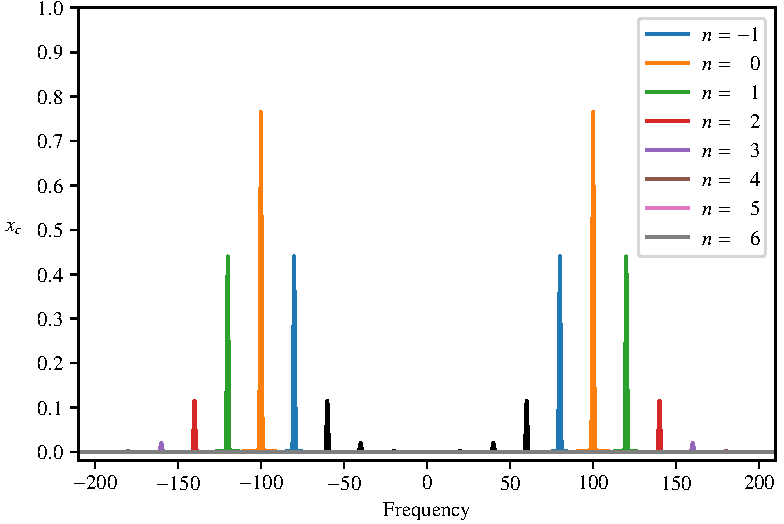
\includegraphics{papers/fm/images/normal.pdf}
	%%% Creator: Matplotlib, PGF backend
%%
%% To include the figure in your LaTeX document, write
%%   \input{<filename>.pgf}
%%
%% Make sure the required packages are loaded in your preamble
%%   \usepackage{pgf}
%%
%% Also ensure that all the required font packages are loaded; for instance,
%% the lmodern package is sometimes necessary when using math font.
%%   \usepackage{lmodern}
%%
%% Figures using additional raster images can only be included by \input if
%% they are in the same directory as the main LaTeX file. For loading figures
%% from other directories you can use the `import` package
%%   \usepackage{import}
%%
%% and then include the figures with
%%   \import{<path to file>}{<filename>.pgf}
%%
%% Matplotlib used the following preamble
%%
\begingroup%
\makeatletter%
\begin{pgfpicture}%
\pgfpathrectangle{\pgfpointorigin}{\pgfqpoint{6.000000in}{4.000000in}}%
\pgfusepath{use as bounding box, clip}%
\begin{pgfscope}%
\pgfsetbuttcap%
\pgfsetmiterjoin%
\pgfsetlinewidth{0.000000pt}%
\definecolor{currentstroke}{rgb}{1.000000,1.000000,1.000000}%
\pgfsetstrokecolor{currentstroke}%
\pgfsetstrokeopacity{0.000000}%
\pgfsetdash{}{0pt}%
\pgfpathmoveto{\pgfqpoint{0.000000in}{0.000000in}}%
\pgfpathlineto{\pgfqpoint{6.000000in}{0.000000in}}%
\pgfpathlineto{\pgfqpoint{6.000000in}{4.000000in}}%
\pgfpathlineto{\pgfqpoint{0.000000in}{4.000000in}}%
\pgfpathlineto{\pgfqpoint{0.000000in}{0.000000in}}%
\pgfpathclose%
\pgfusepath{}%
\end{pgfscope}%
\begin{pgfscope}%
\pgfsetbuttcap%
\pgfsetmiterjoin%
\definecolor{currentfill}{rgb}{1.000000,1.000000,1.000000}%
\pgfsetfillcolor{currentfill}%
\pgfsetlinewidth{0.000000pt}%
\definecolor{currentstroke}{rgb}{0.000000,0.000000,0.000000}%
\pgfsetstrokecolor{currentstroke}%
\pgfsetstrokeopacity{0.000000}%
\pgfsetdash{}{0pt}%
\pgfpathmoveto{\pgfqpoint{0.750000in}{0.500000in}}%
\pgfpathlineto{\pgfqpoint{5.400000in}{0.500000in}}%
\pgfpathlineto{\pgfqpoint{5.400000in}{3.520000in}}%
\pgfpathlineto{\pgfqpoint{0.750000in}{3.520000in}}%
\pgfpathlineto{\pgfqpoint{0.750000in}{0.500000in}}%
\pgfpathclose%
\pgfusepath{fill}%
\end{pgfscope}%
\begin{pgfscope}%
\pgfsetbuttcap%
\pgfsetroundjoin%
\definecolor{currentfill}{rgb}{0.000000,0.000000,0.000000}%
\pgfsetfillcolor{currentfill}%
\pgfsetlinewidth{0.803000pt}%
\definecolor{currentstroke}{rgb}{0.000000,0.000000,0.000000}%
\pgfsetstrokecolor{currentstroke}%
\pgfsetdash{}{0pt}%
\pgfsys@defobject{currentmarker}{\pgfqpoint{0.000000in}{-0.048611in}}{\pgfqpoint{0.000000in}{0.000000in}}{%
\pgfpathmoveto{\pgfqpoint{0.000000in}{0.000000in}}%
\pgfpathlineto{\pgfqpoint{0.000000in}{-0.048611in}}%
\pgfusepath{stroke,fill}%
}%
\begin{pgfscope}%
\pgfsys@transformshift{0.860714in}{0.500000in}%
\pgfsys@useobject{currentmarker}{}%
\end{pgfscope}%
\end{pgfscope}%
\begin{pgfscope}%
\definecolor{textcolor}{rgb}{0.000000,0.000000,0.000000}%
\pgfsetstrokecolor{textcolor}%
\pgfsetfillcolor{textcolor}%
\pgftext[x=0.860714in,y=0.402778in,,top]{\color{textcolor}\rmfamily\fontsize{10.000000}{12.000000}\selectfont \(\displaystyle {\ensuremath{-}200}\)}%
\end{pgfscope}%
\begin{pgfscope}%
\pgfsetbuttcap%
\pgfsetroundjoin%
\definecolor{currentfill}{rgb}{0.000000,0.000000,0.000000}%
\pgfsetfillcolor{currentfill}%
\pgfsetlinewidth{0.803000pt}%
\definecolor{currentstroke}{rgb}{0.000000,0.000000,0.000000}%
\pgfsetstrokecolor{currentstroke}%
\pgfsetdash{}{0pt}%
\pgfsys@defobject{currentmarker}{\pgfqpoint{0.000000in}{-0.048611in}}{\pgfqpoint{0.000000in}{0.000000in}}{%
\pgfpathmoveto{\pgfqpoint{0.000000in}{0.000000in}}%
\pgfpathlineto{\pgfqpoint{0.000000in}{-0.048611in}}%
\pgfusepath{stroke,fill}%
}%
\begin{pgfscope}%
\pgfsys@transformshift{1.414286in}{0.500000in}%
\pgfsys@useobject{currentmarker}{}%
\end{pgfscope}%
\end{pgfscope}%
\begin{pgfscope}%
\definecolor{textcolor}{rgb}{0.000000,0.000000,0.000000}%
\pgfsetstrokecolor{textcolor}%
\pgfsetfillcolor{textcolor}%
\pgftext[x=1.414286in,y=0.402778in,,top]{\color{textcolor}\rmfamily\fontsize{10.000000}{12.000000}\selectfont \(\displaystyle {\ensuremath{-}150}\)}%
\end{pgfscope}%
\begin{pgfscope}%
\pgfsetbuttcap%
\pgfsetroundjoin%
\definecolor{currentfill}{rgb}{0.000000,0.000000,0.000000}%
\pgfsetfillcolor{currentfill}%
\pgfsetlinewidth{0.803000pt}%
\definecolor{currentstroke}{rgb}{0.000000,0.000000,0.000000}%
\pgfsetstrokecolor{currentstroke}%
\pgfsetdash{}{0pt}%
\pgfsys@defobject{currentmarker}{\pgfqpoint{0.000000in}{-0.048611in}}{\pgfqpoint{0.000000in}{0.000000in}}{%
\pgfpathmoveto{\pgfqpoint{0.000000in}{0.000000in}}%
\pgfpathlineto{\pgfqpoint{0.000000in}{-0.048611in}}%
\pgfusepath{stroke,fill}%
}%
\begin{pgfscope}%
\pgfsys@transformshift{1.967857in}{0.500000in}%
\pgfsys@useobject{currentmarker}{}%
\end{pgfscope}%
\end{pgfscope}%
\begin{pgfscope}%
\definecolor{textcolor}{rgb}{0.000000,0.000000,0.000000}%
\pgfsetstrokecolor{textcolor}%
\pgfsetfillcolor{textcolor}%
\pgftext[x=1.967857in,y=0.402778in,,top]{\color{textcolor}\rmfamily\fontsize{10.000000}{12.000000}\selectfont \(\displaystyle {\ensuremath{-}100}\)}%
\end{pgfscope}%
\begin{pgfscope}%
\pgfsetbuttcap%
\pgfsetroundjoin%
\definecolor{currentfill}{rgb}{0.000000,0.000000,0.000000}%
\pgfsetfillcolor{currentfill}%
\pgfsetlinewidth{0.803000pt}%
\definecolor{currentstroke}{rgb}{0.000000,0.000000,0.000000}%
\pgfsetstrokecolor{currentstroke}%
\pgfsetdash{}{0pt}%
\pgfsys@defobject{currentmarker}{\pgfqpoint{0.000000in}{-0.048611in}}{\pgfqpoint{0.000000in}{0.000000in}}{%
\pgfpathmoveto{\pgfqpoint{0.000000in}{0.000000in}}%
\pgfpathlineto{\pgfqpoint{0.000000in}{-0.048611in}}%
\pgfusepath{stroke,fill}%
}%
\begin{pgfscope}%
\pgfsys@transformshift{2.521429in}{0.500000in}%
\pgfsys@useobject{currentmarker}{}%
\end{pgfscope}%
\end{pgfscope}%
\begin{pgfscope}%
\definecolor{textcolor}{rgb}{0.000000,0.000000,0.000000}%
\pgfsetstrokecolor{textcolor}%
\pgfsetfillcolor{textcolor}%
\pgftext[x=2.521429in,y=0.402778in,,top]{\color{textcolor}\rmfamily\fontsize{10.000000}{12.000000}\selectfont \(\displaystyle {\ensuremath{-}50}\)}%
\end{pgfscope}%
\begin{pgfscope}%
\pgfsetbuttcap%
\pgfsetroundjoin%
\definecolor{currentfill}{rgb}{0.000000,0.000000,0.000000}%
\pgfsetfillcolor{currentfill}%
\pgfsetlinewidth{0.803000pt}%
\definecolor{currentstroke}{rgb}{0.000000,0.000000,0.000000}%
\pgfsetstrokecolor{currentstroke}%
\pgfsetdash{}{0pt}%
\pgfsys@defobject{currentmarker}{\pgfqpoint{0.000000in}{-0.048611in}}{\pgfqpoint{0.000000in}{0.000000in}}{%
\pgfpathmoveto{\pgfqpoint{0.000000in}{0.000000in}}%
\pgfpathlineto{\pgfqpoint{0.000000in}{-0.048611in}}%
\pgfusepath{stroke,fill}%
}%
\begin{pgfscope}%
\pgfsys@transformshift{3.075000in}{0.500000in}%
\pgfsys@useobject{currentmarker}{}%
\end{pgfscope}%
\end{pgfscope}%
\begin{pgfscope}%
\definecolor{textcolor}{rgb}{0.000000,0.000000,0.000000}%
\pgfsetstrokecolor{textcolor}%
\pgfsetfillcolor{textcolor}%
\pgftext[x=3.075000in,y=0.402778in,,top]{\color{textcolor}\rmfamily\fontsize{10.000000}{12.000000}\selectfont \(\displaystyle {0}\)}%
\end{pgfscope}%
\begin{pgfscope}%
\pgfsetbuttcap%
\pgfsetroundjoin%
\definecolor{currentfill}{rgb}{0.000000,0.000000,0.000000}%
\pgfsetfillcolor{currentfill}%
\pgfsetlinewidth{0.803000pt}%
\definecolor{currentstroke}{rgb}{0.000000,0.000000,0.000000}%
\pgfsetstrokecolor{currentstroke}%
\pgfsetdash{}{0pt}%
\pgfsys@defobject{currentmarker}{\pgfqpoint{0.000000in}{-0.048611in}}{\pgfqpoint{0.000000in}{0.000000in}}{%
\pgfpathmoveto{\pgfqpoint{0.000000in}{0.000000in}}%
\pgfpathlineto{\pgfqpoint{0.000000in}{-0.048611in}}%
\pgfusepath{stroke,fill}%
}%
\begin{pgfscope}%
\pgfsys@transformshift{3.628571in}{0.500000in}%
\pgfsys@useobject{currentmarker}{}%
\end{pgfscope}%
\end{pgfscope}%
\begin{pgfscope}%
\definecolor{textcolor}{rgb}{0.000000,0.000000,0.000000}%
\pgfsetstrokecolor{textcolor}%
\pgfsetfillcolor{textcolor}%
\pgftext[x=3.628571in,y=0.402778in,,top]{\color{textcolor}\rmfamily\fontsize{10.000000}{12.000000}\selectfont \(\displaystyle {50}\)}%
\end{pgfscope}%
\begin{pgfscope}%
\pgfsetbuttcap%
\pgfsetroundjoin%
\definecolor{currentfill}{rgb}{0.000000,0.000000,0.000000}%
\pgfsetfillcolor{currentfill}%
\pgfsetlinewidth{0.803000pt}%
\definecolor{currentstroke}{rgb}{0.000000,0.000000,0.000000}%
\pgfsetstrokecolor{currentstroke}%
\pgfsetdash{}{0pt}%
\pgfsys@defobject{currentmarker}{\pgfqpoint{0.000000in}{-0.048611in}}{\pgfqpoint{0.000000in}{0.000000in}}{%
\pgfpathmoveto{\pgfqpoint{0.000000in}{0.000000in}}%
\pgfpathlineto{\pgfqpoint{0.000000in}{-0.048611in}}%
\pgfusepath{stroke,fill}%
}%
\begin{pgfscope}%
\pgfsys@transformshift{4.182143in}{0.500000in}%
\pgfsys@useobject{currentmarker}{}%
\end{pgfscope}%
\end{pgfscope}%
\begin{pgfscope}%
\definecolor{textcolor}{rgb}{0.000000,0.000000,0.000000}%
\pgfsetstrokecolor{textcolor}%
\pgfsetfillcolor{textcolor}%
\pgftext[x=4.182143in,y=0.402778in,,top]{\color{textcolor}\rmfamily\fontsize{10.000000}{12.000000}\selectfont \(\displaystyle {100}\)}%
\end{pgfscope}%
\begin{pgfscope}%
\pgfsetbuttcap%
\pgfsetroundjoin%
\definecolor{currentfill}{rgb}{0.000000,0.000000,0.000000}%
\pgfsetfillcolor{currentfill}%
\pgfsetlinewidth{0.803000pt}%
\definecolor{currentstroke}{rgb}{0.000000,0.000000,0.000000}%
\pgfsetstrokecolor{currentstroke}%
\pgfsetdash{}{0pt}%
\pgfsys@defobject{currentmarker}{\pgfqpoint{0.000000in}{-0.048611in}}{\pgfqpoint{0.000000in}{0.000000in}}{%
\pgfpathmoveto{\pgfqpoint{0.000000in}{0.000000in}}%
\pgfpathlineto{\pgfqpoint{0.000000in}{-0.048611in}}%
\pgfusepath{stroke,fill}%
}%
\begin{pgfscope}%
\pgfsys@transformshift{4.735714in}{0.500000in}%
\pgfsys@useobject{currentmarker}{}%
\end{pgfscope}%
\end{pgfscope}%
\begin{pgfscope}%
\definecolor{textcolor}{rgb}{0.000000,0.000000,0.000000}%
\pgfsetstrokecolor{textcolor}%
\pgfsetfillcolor{textcolor}%
\pgftext[x=4.735714in,y=0.402778in,,top]{\color{textcolor}\rmfamily\fontsize{10.000000}{12.000000}\selectfont \(\displaystyle {150}\)}%
\end{pgfscope}%
\begin{pgfscope}%
\pgfsetbuttcap%
\pgfsetroundjoin%
\definecolor{currentfill}{rgb}{0.000000,0.000000,0.000000}%
\pgfsetfillcolor{currentfill}%
\pgfsetlinewidth{0.803000pt}%
\definecolor{currentstroke}{rgb}{0.000000,0.000000,0.000000}%
\pgfsetstrokecolor{currentstroke}%
\pgfsetdash{}{0pt}%
\pgfsys@defobject{currentmarker}{\pgfqpoint{0.000000in}{-0.048611in}}{\pgfqpoint{0.000000in}{0.000000in}}{%
\pgfpathmoveto{\pgfqpoint{0.000000in}{0.000000in}}%
\pgfpathlineto{\pgfqpoint{0.000000in}{-0.048611in}}%
\pgfusepath{stroke,fill}%
}%
\begin{pgfscope}%
\pgfsys@transformshift{5.289286in}{0.500000in}%
\pgfsys@useobject{currentmarker}{}%
\end{pgfscope}%
\end{pgfscope}%
\begin{pgfscope}%
\definecolor{textcolor}{rgb}{0.000000,0.000000,0.000000}%
\pgfsetstrokecolor{textcolor}%
\pgfsetfillcolor{textcolor}%
\pgftext[x=5.289286in,y=0.402778in,,top]{\color{textcolor}\rmfamily\fontsize{10.000000}{12.000000}\selectfont \(\displaystyle {200}\)}%
\end{pgfscope}%
\begin{pgfscope}%
\definecolor{textcolor}{rgb}{0.000000,0.000000,0.000000}%
\pgfsetstrokecolor{textcolor}%
\pgfsetfillcolor{textcolor}%
\pgftext[x=3.075000in,y=0.223766in,,top]{\color{textcolor}\rmfamily\fontsize{10.000000}{12.000000}\selectfont Frequency}%
\end{pgfscope}%
\begin{pgfscope}%
\pgfsetbuttcap%
\pgfsetroundjoin%
\definecolor{currentfill}{rgb}{0.000000,0.000000,0.000000}%
\pgfsetfillcolor{currentfill}%
\pgfsetlinewidth{0.803000pt}%
\definecolor{currentstroke}{rgb}{0.000000,0.000000,0.000000}%
\pgfsetstrokecolor{currentstroke}%
\pgfsetdash{}{0pt}%
\pgfsys@defobject{currentmarker}{\pgfqpoint{-0.048611in}{0.000000in}}{\pgfqpoint{-0.000000in}{0.000000in}}{%
\pgfpathmoveto{\pgfqpoint{-0.000000in}{0.000000in}}%
\pgfpathlineto{\pgfqpoint{-0.048611in}{0.000000in}}%
\pgfusepath{stroke,fill}%
}%
\begin{pgfscope}%
\pgfsys@transformshift{0.750000in}{0.559216in}%
\pgfsys@useobject{currentmarker}{}%
\end{pgfscope}%
\end{pgfscope}%
\begin{pgfscope}%
\definecolor{textcolor}{rgb}{0.000000,0.000000,0.000000}%
\pgfsetstrokecolor{textcolor}%
\pgfsetfillcolor{textcolor}%
\pgftext[x=0.475308in, y=0.510990in, left, base]{\color{textcolor}\rmfamily\fontsize{10.000000}{12.000000}\selectfont \(\displaystyle {0.0}\)}%
\end{pgfscope}%
\begin{pgfscope}%
\pgfsetbuttcap%
\pgfsetroundjoin%
\definecolor{currentfill}{rgb}{0.000000,0.000000,0.000000}%
\pgfsetfillcolor{currentfill}%
\pgfsetlinewidth{0.803000pt}%
\definecolor{currentstroke}{rgb}{0.000000,0.000000,0.000000}%
\pgfsetstrokecolor{currentstroke}%
\pgfsetdash{}{0pt}%
\pgfsys@defobject{currentmarker}{\pgfqpoint{-0.048611in}{0.000000in}}{\pgfqpoint{-0.000000in}{0.000000in}}{%
\pgfpathmoveto{\pgfqpoint{-0.000000in}{0.000000in}}%
\pgfpathlineto{\pgfqpoint{-0.048611in}{0.000000in}}%
\pgfusepath{stroke,fill}%
}%
\begin{pgfscope}%
\pgfsys@transformshift{0.750000in}{0.855294in}%
\pgfsys@useobject{currentmarker}{}%
\end{pgfscope}%
\end{pgfscope}%
\begin{pgfscope}%
\definecolor{textcolor}{rgb}{0.000000,0.000000,0.000000}%
\pgfsetstrokecolor{textcolor}%
\pgfsetfillcolor{textcolor}%
\pgftext[x=0.475308in, y=0.807069in, left, base]{\color{textcolor}\rmfamily\fontsize{10.000000}{12.000000}\selectfont \(\displaystyle {0.1}\)}%
\end{pgfscope}%
\begin{pgfscope}%
\pgfsetbuttcap%
\pgfsetroundjoin%
\definecolor{currentfill}{rgb}{0.000000,0.000000,0.000000}%
\pgfsetfillcolor{currentfill}%
\pgfsetlinewidth{0.803000pt}%
\definecolor{currentstroke}{rgb}{0.000000,0.000000,0.000000}%
\pgfsetstrokecolor{currentstroke}%
\pgfsetdash{}{0pt}%
\pgfsys@defobject{currentmarker}{\pgfqpoint{-0.048611in}{0.000000in}}{\pgfqpoint{-0.000000in}{0.000000in}}{%
\pgfpathmoveto{\pgfqpoint{-0.000000in}{0.000000in}}%
\pgfpathlineto{\pgfqpoint{-0.048611in}{0.000000in}}%
\pgfusepath{stroke,fill}%
}%
\begin{pgfscope}%
\pgfsys@transformshift{0.750000in}{1.151373in}%
\pgfsys@useobject{currentmarker}{}%
\end{pgfscope}%
\end{pgfscope}%
\begin{pgfscope}%
\definecolor{textcolor}{rgb}{0.000000,0.000000,0.000000}%
\pgfsetstrokecolor{textcolor}%
\pgfsetfillcolor{textcolor}%
\pgftext[x=0.475308in, y=1.103147in, left, base]{\color{textcolor}\rmfamily\fontsize{10.000000}{12.000000}\selectfont \(\displaystyle {0.2}\)}%
\end{pgfscope}%
\begin{pgfscope}%
\pgfsetbuttcap%
\pgfsetroundjoin%
\definecolor{currentfill}{rgb}{0.000000,0.000000,0.000000}%
\pgfsetfillcolor{currentfill}%
\pgfsetlinewidth{0.803000pt}%
\definecolor{currentstroke}{rgb}{0.000000,0.000000,0.000000}%
\pgfsetstrokecolor{currentstroke}%
\pgfsetdash{}{0pt}%
\pgfsys@defobject{currentmarker}{\pgfqpoint{-0.048611in}{0.000000in}}{\pgfqpoint{-0.000000in}{0.000000in}}{%
\pgfpathmoveto{\pgfqpoint{-0.000000in}{0.000000in}}%
\pgfpathlineto{\pgfqpoint{-0.048611in}{0.000000in}}%
\pgfusepath{stroke,fill}%
}%
\begin{pgfscope}%
\pgfsys@transformshift{0.750000in}{1.447451in}%
\pgfsys@useobject{currentmarker}{}%
\end{pgfscope}%
\end{pgfscope}%
\begin{pgfscope}%
\definecolor{textcolor}{rgb}{0.000000,0.000000,0.000000}%
\pgfsetstrokecolor{textcolor}%
\pgfsetfillcolor{textcolor}%
\pgftext[x=0.475308in, y=1.399226in, left, base]{\color{textcolor}\rmfamily\fontsize{10.000000}{12.000000}\selectfont \(\displaystyle {0.3}\)}%
\end{pgfscope}%
\begin{pgfscope}%
\pgfsetbuttcap%
\pgfsetroundjoin%
\definecolor{currentfill}{rgb}{0.000000,0.000000,0.000000}%
\pgfsetfillcolor{currentfill}%
\pgfsetlinewidth{0.803000pt}%
\definecolor{currentstroke}{rgb}{0.000000,0.000000,0.000000}%
\pgfsetstrokecolor{currentstroke}%
\pgfsetdash{}{0pt}%
\pgfsys@defobject{currentmarker}{\pgfqpoint{-0.048611in}{0.000000in}}{\pgfqpoint{-0.000000in}{0.000000in}}{%
\pgfpathmoveto{\pgfqpoint{-0.000000in}{0.000000in}}%
\pgfpathlineto{\pgfqpoint{-0.048611in}{0.000000in}}%
\pgfusepath{stroke,fill}%
}%
\begin{pgfscope}%
\pgfsys@transformshift{0.750000in}{1.743529in}%
\pgfsys@useobject{currentmarker}{}%
\end{pgfscope}%
\end{pgfscope}%
\begin{pgfscope}%
\definecolor{textcolor}{rgb}{0.000000,0.000000,0.000000}%
\pgfsetstrokecolor{textcolor}%
\pgfsetfillcolor{textcolor}%
\pgftext[x=0.475308in, y=1.695304in, left, base]{\color{textcolor}\rmfamily\fontsize{10.000000}{12.000000}\selectfont \(\displaystyle {0.4}\)}%
\end{pgfscope}%
\begin{pgfscope}%
\pgfsetbuttcap%
\pgfsetroundjoin%
\definecolor{currentfill}{rgb}{0.000000,0.000000,0.000000}%
\pgfsetfillcolor{currentfill}%
\pgfsetlinewidth{0.803000pt}%
\definecolor{currentstroke}{rgb}{0.000000,0.000000,0.000000}%
\pgfsetstrokecolor{currentstroke}%
\pgfsetdash{}{0pt}%
\pgfsys@defobject{currentmarker}{\pgfqpoint{-0.048611in}{0.000000in}}{\pgfqpoint{-0.000000in}{0.000000in}}{%
\pgfpathmoveto{\pgfqpoint{-0.000000in}{0.000000in}}%
\pgfpathlineto{\pgfqpoint{-0.048611in}{0.000000in}}%
\pgfusepath{stroke,fill}%
}%
\begin{pgfscope}%
\pgfsys@transformshift{0.750000in}{2.039608in}%
\pgfsys@useobject{currentmarker}{}%
\end{pgfscope}%
\end{pgfscope}%
\begin{pgfscope}%
\definecolor{textcolor}{rgb}{0.000000,0.000000,0.000000}%
\pgfsetstrokecolor{textcolor}%
\pgfsetfillcolor{textcolor}%
\pgftext[x=0.475308in, y=1.991383in, left, base]{\color{textcolor}\rmfamily\fontsize{10.000000}{12.000000}\selectfont \(\displaystyle {0.5}\)}%
\end{pgfscope}%
\begin{pgfscope}%
\pgfsetbuttcap%
\pgfsetroundjoin%
\definecolor{currentfill}{rgb}{0.000000,0.000000,0.000000}%
\pgfsetfillcolor{currentfill}%
\pgfsetlinewidth{0.803000pt}%
\definecolor{currentstroke}{rgb}{0.000000,0.000000,0.000000}%
\pgfsetstrokecolor{currentstroke}%
\pgfsetdash{}{0pt}%
\pgfsys@defobject{currentmarker}{\pgfqpoint{-0.048611in}{0.000000in}}{\pgfqpoint{-0.000000in}{0.000000in}}{%
\pgfpathmoveto{\pgfqpoint{-0.000000in}{0.000000in}}%
\pgfpathlineto{\pgfqpoint{-0.048611in}{0.000000in}}%
\pgfusepath{stroke,fill}%
}%
\begin{pgfscope}%
\pgfsys@transformshift{0.750000in}{2.335686in}%
\pgfsys@useobject{currentmarker}{}%
\end{pgfscope}%
\end{pgfscope}%
\begin{pgfscope}%
\definecolor{textcolor}{rgb}{0.000000,0.000000,0.000000}%
\pgfsetstrokecolor{textcolor}%
\pgfsetfillcolor{textcolor}%
\pgftext[x=0.475308in, y=2.287461in, left, base]{\color{textcolor}\rmfamily\fontsize{10.000000}{12.000000}\selectfont \(\displaystyle {0.6}\)}%
\end{pgfscope}%
\begin{pgfscope}%
\pgfsetbuttcap%
\pgfsetroundjoin%
\definecolor{currentfill}{rgb}{0.000000,0.000000,0.000000}%
\pgfsetfillcolor{currentfill}%
\pgfsetlinewidth{0.803000pt}%
\definecolor{currentstroke}{rgb}{0.000000,0.000000,0.000000}%
\pgfsetstrokecolor{currentstroke}%
\pgfsetdash{}{0pt}%
\pgfsys@defobject{currentmarker}{\pgfqpoint{-0.048611in}{0.000000in}}{\pgfqpoint{-0.000000in}{0.000000in}}{%
\pgfpathmoveto{\pgfqpoint{-0.000000in}{0.000000in}}%
\pgfpathlineto{\pgfqpoint{-0.048611in}{0.000000in}}%
\pgfusepath{stroke,fill}%
}%
\begin{pgfscope}%
\pgfsys@transformshift{0.750000in}{2.631765in}%
\pgfsys@useobject{currentmarker}{}%
\end{pgfscope}%
\end{pgfscope}%
\begin{pgfscope}%
\definecolor{textcolor}{rgb}{0.000000,0.000000,0.000000}%
\pgfsetstrokecolor{textcolor}%
\pgfsetfillcolor{textcolor}%
\pgftext[x=0.475308in, y=2.583539in, left, base]{\color{textcolor}\rmfamily\fontsize{10.000000}{12.000000}\selectfont \(\displaystyle {0.7}\)}%
\end{pgfscope}%
\begin{pgfscope}%
\pgfsetbuttcap%
\pgfsetroundjoin%
\definecolor{currentfill}{rgb}{0.000000,0.000000,0.000000}%
\pgfsetfillcolor{currentfill}%
\pgfsetlinewidth{0.803000pt}%
\definecolor{currentstroke}{rgb}{0.000000,0.000000,0.000000}%
\pgfsetstrokecolor{currentstroke}%
\pgfsetdash{}{0pt}%
\pgfsys@defobject{currentmarker}{\pgfqpoint{-0.048611in}{0.000000in}}{\pgfqpoint{-0.000000in}{0.000000in}}{%
\pgfpathmoveto{\pgfqpoint{-0.000000in}{0.000000in}}%
\pgfpathlineto{\pgfqpoint{-0.048611in}{0.000000in}}%
\pgfusepath{stroke,fill}%
}%
\begin{pgfscope}%
\pgfsys@transformshift{0.750000in}{2.927843in}%
\pgfsys@useobject{currentmarker}{}%
\end{pgfscope}%
\end{pgfscope}%
\begin{pgfscope}%
\definecolor{textcolor}{rgb}{0.000000,0.000000,0.000000}%
\pgfsetstrokecolor{textcolor}%
\pgfsetfillcolor{textcolor}%
\pgftext[x=0.475308in, y=2.879618in, left, base]{\color{textcolor}\rmfamily\fontsize{10.000000}{12.000000}\selectfont \(\displaystyle {0.8}\)}%
\end{pgfscope}%
\begin{pgfscope}%
\pgfsetbuttcap%
\pgfsetroundjoin%
\definecolor{currentfill}{rgb}{0.000000,0.000000,0.000000}%
\pgfsetfillcolor{currentfill}%
\pgfsetlinewidth{0.803000pt}%
\definecolor{currentstroke}{rgb}{0.000000,0.000000,0.000000}%
\pgfsetstrokecolor{currentstroke}%
\pgfsetdash{}{0pt}%
\pgfsys@defobject{currentmarker}{\pgfqpoint{-0.048611in}{0.000000in}}{\pgfqpoint{-0.000000in}{0.000000in}}{%
\pgfpathmoveto{\pgfqpoint{-0.000000in}{0.000000in}}%
\pgfpathlineto{\pgfqpoint{-0.048611in}{0.000000in}}%
\pgfusepath{stroke,fill}%
}%
\begin{pgfscope}%
\pgfsys@transformshift{0.750000in}{3.223922in}%
\pgfsys@useobject{currentmarker}{}%
\end{pgfscope}%
\end{pgfscope}%
\begin{pgfscope}%
\definecolor{textcolor}{rgb}{0.000000,0.000000,0.000000}%
\pgfsetstrokecolor{textcolor}%
\pgfsetfillcolor{textcolor}%
\pgftext[x=0.475308in, y=3.175696in, left, base]{\color{textcolor}\rmfamily\fontsize{10.000000}{12.000000}\selectfont \(\displaystyle {0.9}\)}%
\end{pgfscope}%
\begin{pgfscope}%
\pgfsetbuttcap%
\pgfsetroundjoin%
\definecolor{currentfill}{rgb}{0.000000,0.000000,0.000000}%
\pgfsetfillcolor{currentfill}%
\pgfsetlinewidth{0.803000pt}%
\definecolor{currentstroke}{rgb}{0.000000,0.000000,0.000000}%
\pgfsetstrokecolor{currentstroke}%
\pgfsetdash{}{0pt}%
\pgfsys@defobject{currentmarker}{\pgfqpoint{-0.048611in}{0.000000in}}{\pgfqpoint{-0.000000in}{0.000000in}}{%
\pgfpathmoveto{\pgfqpoint{-0.000000in}{0.000000in}}%
\pgfpathlineto{\pgfqpoint{-0.048611in}{0.000000in}}%
\pgfusepath{stroke,fill}%
}%
\begin{pgfscope}%
\pgfsys@transformshift{0.750000in}{3.520000in}%
\pgfsys@useobject{currentmarker}{}%
\end{pgfscope}%
\end{pgfscope}%
\begin{pgfscope}%
\definecolor{textcolor}{rgb}{0.000000,0.000000,0.000000}%
\pgfsetstrokecolor{textcolor}%
\pgfsetfillcolor{textcolor}%
\pgftext[x=0.475308in, y=3.471775in, left, base]{\color{textcolor}\rmfamily\fontsize{10.000000}{12.000000}\selectfont \(\displaystyle {1.0}\)}%
\end{pgfscope}%
\begin{pgfscope}%
\definecolor{textcolor}{rgb}{0.000000,0.000000,0.000000}%
\pgfsetstrokecolor{textcolor}%
\pgfsetfillcolor{textcolor}%
\pgftext[x=0.419753in,y=2.010000in,,bottom,rotate=90.000000]{\color{textcolor}\rmfamily\fontsize{10.000000}{12.000000}\selectfont \(\displaystyle x_c\)}%
\end{pgfscope}%
\begin{pgfscope}%
\pgfpathrectangle{\pgfqpoint{0.750000in}{0.500000in}}{\pgfqpoint{4.650000in}{3.020000in}}%
\pgfusepath{clip}%
\pgfsetrectcap%
\pgfsetroundjoin%
\pgfsetlinewidth{1.505625pt}%
\definecolor{currentstroke}{rgb}{0.000000,0.000000,0.000000}%
\pgfsetstrokecolor{currentstroke}%
\pgfsetdash{}{0pt}%
\pgfpathmoveto{\pgfqpoint{3.075000in}{0.559216in}}%
\pgfpathlineto{\pgfqpoint{5.413889in}{0.559216in}}%
\pgfpathmoveto{\pgfqpoint{5.413889in}{0.559216in}}%
\pgfpathlineto{\pgfqpoint{0.736111in}{0.559216in}}%
\pgfpathmoveto{\pgfqpoint{0.736111in}{0.559216in}}%
\pgfpathlineto{\pgfqpoint{3.063929in}{0.559216in}}%
\pgfpathlineto{\pgfqpoint{3.063929in}{0.559216in}}%
\pgfusepath{stroke}%
\end{pgfscope}%
\begin{pgfscope}%
\pgfpathrectangle{\pgfqpoint{0.750000in}{0.500000in}}{\pgfqpoint{4.650000in}{3.020000in}}%
\pgfusepath{clip}%
\pgfsetrectcap%
\pgfsetroundjoin%
\pgfsetlinewidth{1.505625pt}%
\definecolor{currentstroke}{rgb}{0.000000,0.000000,0.000000}%
\pgfsetstrokecolor{currentstroke}%
\pgfsetdash{}{0pt}%
\pgfpathmoveto{\pgfqpoint{3.075000in}{0.559216in}}%
\pgfpathlineto{\pgfqpoint{5.413889in}{0.559216in}}%
\pgfpathmoveto{\pgfqpoint{5.413889in}{0.559216in}}%
\pgfpathlineto{\pgfqpoint{0.736111in}{0.559216in}}%
\pgfpathmoveto{\pgfqpoint{0.736111in}{0.559216in}}%
\pgfpathlineto{\pgfqpoint{3.063929in}{0.559216in}}%
\pgfpathlineto{\pgfqpoint{3.063929in}{0.559216in}}%
\pgfusepath{stroke}%
\end{pgfscope}%
\begin{pgfscope}%
\pgfpathrectangle{\pgfqpoint{0.750000in}{0.500000in}}{\pgfqpoint{4.650000in}{3.020000in}}%
\pgfusepath{clip}%
\pgfsetrectcap%
\pgfsetroundjoin%
\pgfsetlinewidth{1.505625pt}%
\definecolor{currentstroke}{rgb}{0.000000,0.000000,0.000000}%
\pgfsetstrokecolor{currentstroke}%
\pgfsetdash{}{0pt}%
\pgfpathmoveto{\pgfqpoint{3.075000in}{0.559217in}}%
\pgfpathlineto{\pgfqpoint{3.285357in}{0.559231in}}%
\pgfpathlineto{\pgfqpoint{3.296429in}{0.566549in}}%
\pgfpathlineto{\pgfqpoint{3.307500in}{0.559230in}}%
\pgfpathlineto{\pgfqpoint{5.413889in}{0.559216in}}%
\pgfpathmoveto{\pgfqpoint{5.413889in}{0.559216in}}%
\pgfpathlineto{\pgfqpoint{0.736111in}{0.559216in}}%
\pgfpathmoveto{\pgfqpoint{0.736111in}{0.559216in}}%
\pgfpathlineto{\pgfqpoint{2.842500in}{0.559230in}}%
\pgfpathlineto{\pgfqpoint{2.853571in}{0.566549in}}%
\pgfpathlineto{\pgfqpoint{2.864643in}{0.559231in}}%
\pgfpathlineto{\pgfqpoint{3.063929in}{0.559217in}}%
\pgfpathlineto{\pgfqpoint{3.063929in}{0.559217in}}%
\pgfusepath{stroke}%
\end{pgfscope}%
\begin{pgfscope}%
\pgfpathrectangle{\pgfqpoint{0.750000in}{0.500000in}}{\pgfqpoint{4.650000in}{3.020000in}}%
\pgfusepath{clip}%
\pgfsetrectcap%
\pgfsetroundjoin%
\pgfsetlinewidth{1.505625pt}%
\definecolor{currentstroke}{rgb}{0.000000,0.000000,0.000000}%
\pgfsetstrokecolor{currentstroke}%
\pgfsetdash{}{0pt}%
\pgfpathmoveto{\pgfqpoint{3.075000in}{0.559222in}}%
\pgfpathlineto{\pgfqpoint{3.506786in}{0.559446in}}%
\pgfpathlineto{\pgfqpoint{3.517857in}{0.617136in}}%
\pgfpathlineto{\pgfqpoint{3.528929in}{0.559449in}}%
\pgfpathlineto{\pgfqpoint{3.695000in}{0.559231in}}%
\pgfpathlineto{\pgfqpoint{5.413889in}{0.559218in}}%
\pgfpathmoveto{\pgfqpoint{5.413889in}{0.559216in}}%
\pgfpathlineto{\pgfqpoint{0.736111in}{0.559216in}}%
\pgfpathmoveto{\pgfqpoint{0.736111in}{0.559218in}}%
\pgfpathlineto{\pgfqpoint{2.621071in}{0.559449in}}%
\pgfpathlineto{\pgfqpoint{2.632143in}{0.617136in}}%
\pgfpathlineto{\pgfqpoint{2.643214in}{0.559446in}}%
\pgfpathlineto{\pgfqpoint{2.809286in}{0.559229in}}%
\pgfpathlineto{\pgfqpoint{3.063929in}{0.559223in}}%
\pgfpathlineto{\pgfqpoint{3.063929in}{0.559223in}}%
\pgfusepath{stroke}%
\end{pgfscope}%
\begin{pgfscope}%
\pgfpathrectangle{\pgfqpoint{0.750000in}{0.500000in}}{\pgfqpoint{4.650000in}{3.020000in}}%
\pgfusepath{clip}%
\pgfsetrectcap%
\pgfsetroundjoin%
\pgfsetlinewidth{1.505625pt}%
\definecolor{currentstroke}{rgb}{0.000000,0.000000,0.000000}%
\pgfsetstrokecolor{currentstroke}%
\pgfsetdash{}{0pt}%
\pgfpathmoveto{\pgfqpoint{3.075000in}{0.559256in}}%
\pgfpathlineto{\pgfqpoint{3.717143in}{0.560228in}}%
\pgfpathlineto{\pgfqpoint{3.728214in}{0.561240in}}%
\pgfpathlineto{\pgfqpoint{3.739286in}{0.899395in}}%
\pgfpathlineto{\pgfqpoint{3.750357in}{0.561275in}}%
\pgfpathlineto{\pgfqpoint{3.783571in}{0.559732in}}%
\pgfpathlineto{\pgfqpoint{3.993929in}{0.559310in}}%
\pgfpathlineto{\pgfqpoint{5.413889in}{0.559233in}}%
\pgfpathmoveto{\pgfqpoint{5.413889in}{0.559217in}}%
\pgfpathlineto{\pgfqpoint{0.736111in}{0.559217in}}%
\pgfpathmoveto{\pgfqpoint{0.736111in}{0.559233in}}%
\pgfpathlineto{\pgfqpoint{2.388571in}{0.560245in}}%
\pgfpathlineto{\pgfqpoint{2.399643in}{0.561275in}}%
\pgfpathlineto{\pgfqpoint{2.410714in}{0.899395in}}%
\pgfpathlineto{\pgfqpoint{2.421786in}{0.561240in}}%
\pgfpathlineto{\pgfqpoint{2.455000in}{0.559720in}}%
\pgfpathlineto{\pgfqpoint{2.665357in}{0.559300in}}%
\pgfpathlineto{\pgfqpoint{3.063929in}{0.559256in}}%
\pgfpathlineto{\pgfqpoint{3.063929in}{0.559256in}}%
\pgfusepath{stroke}%
\end{pgfscope}%
\begin{pgfscope}%
\pgfpathrectangle{\pgfqpoint{0.750000in}{0.500000in}}{\pgfqpoint{4.650000in}{3.020000in}}%
\pgfusepath{clip}%
\pgfsetrectcap%
\pgfsetroundjoin%
\pgfsetlinewidth{1.505625pt}%
\definecolor{currentstroke}{rgb}{0.121569,0.466667,0.705882}%
\pgfsetstrokecolor{currentstroke}%
\pgfsetdash{}{0pt}%
\pgfpathmoveto{\pgfqpoint{3.075000in}{0.559464in}}%
\pgfpathlineto{\pgfqpoint{3.894286in}{0.561006in}}%
\pgfpathlineto{\pgfqpoint{3.927500in}{0.562735in}}%
\pgfpathlineto{\pgfqpoint{3.938571in}{0.564460in}}%
\pgfpathlineto{\pgfqpoint{3.949643in}{0.569609in}}%
\pgfpathlineto{\pgfqpoint{3.960714in}{1.862026in}}%
\pgfpathlineto{\pgfqpoint{3.971786in}{0.569671in}}%
\pgfpathlineto{\pgfqpoint{3.982857in}{0.564396in}}%
\pgfpathlineto{\pgfqpoint{4.005000in}{0.561776in}}%
\pgfpathlineto{\pgfqpoint{4.060357in}{0.560326in}}%
\pgfpathlineto{\pgfqpoint{4.281786in}{0.559532in}}%
\pgfpathlineto{\pgfqpoint{5.413889in}{0.559270in}}%
\pgfpathmoveto{\pgfqpoint{5.413889in}{0.559218in}}%
\pgfpathlineto{\pgfqpoint{0.736111in}{0.559218in}}%
\pgfpathmoveto{\pgfqpoint{0.736111in}{0.559270in}}%
\pgfpathlineto{\pgfqpoint{2.111786in}{0.560656in}}%
\pgfpathlineto{\pgfqpoint{2.156071in}{0.562648in}}%
\pgfpathlineto{\pgfqpoint{2.167143in}{0.564396in}}%
\pgfpathlineto{\pgfqpoint{2.178214in}{0.569671in}}%
\pgfpathlineto{\pgfqpoint{2.189286in}{1.862026in}}%
\pgfpathlineto{\pgfqpoint{2.200357in}{0.569609in}}%
\pgfpathlineto{\pgfqpoint{2.211429in}{0.564460in}}%
\pgfpathlineto{\pgfqpoint{2.233571in}{0.561871in}}%
\pgfpathlineto{\pgfqpoint{2.288929in}{0.560429in}}%
\pgfpathlineto{\pgfqpoint{2.510357in}{0.559642in}}%
\pgfpathlineto{\pgfqpoint{3.063929in}{0.559464in}}%
\pgfpathlineto{\pgfqpoint{3.063929in}{0.559464in}}%
\pgfusepath{stroke}%
\end{pgfscope}%
\begin{pgfscope}%
\pgfpathrectangle{\pgfqpoint{0.750000in}{0.500000in}}{\pgfqpoint{4.650000in}{3.020000in}}%
\pgfusepath{clip}%
\pgfsetrectcap%
\pgfsetroundjoin%
\pgfsetlinewidth{1.505625pt}%
\definecolor{currentstroke}{rgb}{1.000000,0.498039,0.054902}%
\pgfsetstrokecolor{currentstroke}%
\pgfsetdash{}{0pt}%
\pgfpathmoveto{\pgfqpoint{3.075000in}{0.559216in}}%
\pgfpathlineto{\pgfqpoint{4.060357in}{0.561153in}}%
\pgfpathlineto{\pgfqpoint{4.126786in}{0.563621in}}%
\pgfpathlineto{\pgfqpoint{4.148929in}{0.566627in}}%
\pgfpathlineto{\pgfqpoint{4.160000in}{0.570372in}}%
\pgfpathlineto{\pgfqpoint{4.171071in}{0.581532in}}%
\pgfpathlineto{\pgfqpoint{4.182143in}{2.824315in}}%
\pgfpathlineto{\pgfqpoint{4.193214in}{0.582212in}}%
\pgfpathlineto{\pgfqpoint{4.204286in}{0.570712in}}%
\pgfpathlineto{\pgfqpoint{4.215357in}{0.566904in}}%
\pgfpathlineto{\pgfqpoint{4.237500in}{0.563866in}}%
\pgfpathlineto{\pgfqpoint{4.292857in}{0.561591in}}%
\pgfpathlineto{\pgfqpoint{4.436786in}{0.560303in}}%
\pgfpathlineto{\pgfqpoint{5.034643in}{0.559592in}}%
\pgfpathlineto{\pgfqpoint{5.413889in}{0.559492in}}%
\pgfpathmoveto{\pgfqpoint{5.413889in}{0.559230in}}%
\pgfpathlineto{\pgfqpoint{0.736111in}{0.559230in}}%
\pgfpathmoveto{\pgfqpoint{0.736111in}{0.559492in}}%
\pgfpathlineto{\pgfqpoint{1.835000in}{0.561212in}}%
\pgfpathlineto{\pgfqpoint{1.912500in}{0.563866in}}%
\pgfpathlineto{\pgfqpoint{1.934643in}{0.566904in}}%
\pgfpathlineto{\pgfqpoint{1.945714in}{0.570712in}}%
\pgfpathlineto{\pgfqpoint{1.956786in}{0.582212in}}%
\pgfpathlineto{\pgfqpoint{1.967857in}{2.824315in}}%
\pgfpathlineto{\pgfqpoint{1.978929in}{0.581532in}}%
\pgfpathlineto{\pgfqpoint{1.990000in}{0.570372in}}%
\pgfpathlineto{\pgfqpoint{2.001071in}{0.566627in}}%
\pgfpathlineto{\pgfqpoint{2.023214in}{0.563621in}}%
\pgfpathlineto{\pgfqpoint{2.078571in}{0.561360in}}%
\pgfpathlineto{\pgfqpoint{2.222500in}{0.560072in}}%
\pgfpathlineto{\pgfqpoint{2.820357in}{0.559326in}}%
\pgfpathlineto{\pgfqpoint{3.063929in}{0.559220in}}%
\pgfpathlineto{\pgfqpoint{3.063929in}{0.559220in}}%
\pgfusepath{stroke}%
\end{pgfscope}%
\begin{pgfscope}%
\pgfpathrectangle{\pgfqpoint{0.750000in}{0.500000in}}{\pgfqpoint{4.650000in}{3.020000in}}%
\pgfusepath{clip}%
\pgfsetrectcap%
\pgfsetroundjoin%
\pgfsetlinewidth{1.505625pt}%
\definecolor{currentstroke}{rgb}{0.172549,0.627451,0.172549}%
\pgfsetstrokecolor{currentstroke}%
\pgfsetdash{}{0pt}%
\pgfpathmoveto{\pgfqpoint{3.075000in}{0.559464in}}%
\pgfpathlineto{\pgfqpoint{4.303929in}{0.561006in}}%
\pgfpathlineto{\pgfqpoint{4.359286in}{0.563166in}}%
\pgfpathlineto{\pgfqpoint{4.381429in}{0.567039in}}%
\pgfpathlineto{\pgfqpoint{4.392500in}{0.574716in}}%
\pgfpathlineto{\pgfqpoint{4.403571in}{1.861855in}}%
\pgfpathlineto{\pgfqpoint{4.414643in}{0.574986in}}%
\pgfpathlineto{\pgfqpoint{4.425714in}{0.567027in}}%
\pgfpathlineto{\pgfqpoint{4.447857in}{0.563084in}}%
\pgfpathlineto{\pgfqpoint{4.492143in}{0.561122in}}%
\pgfpathlineto{\pgfqpoint{4.625000in}{0.559950in}}%
\pgfpathlineto{\pgfqpoint{5.256071in}{0.559381in}}%
\pgfpathlineto{\pgfqpoint{5.413889in}{0.559352in}}%
\pgfpathmoveto{\pgfqpoint{5.413889in}{0.559219in}}%
\pgfpathlineto{\pgfqpoint{0.736111in}{0.559219in}}%
\pgfpathmoveto{\pgfqpoint{0.736111in}{0.559352in}}%
\pgfpathlineto{\pgfqpoint{1.646786in}{0.560905in}}%
\pgfpathlineto{\pgfqpoint{1.702143in}{0.563084in}}%
\pgfpathlineto{\pgfqpoint{1.724286in}{0.567027in}}%
\pgfpathlineto{\pgfqpoint{1.735357in}{0.574986in}}%
\pgfpathlineto{\pgfqpoint{1.746429in}{1.861855in}}%
\pgfpathlineto{\pgfqpoint{1.757500in}{0.574716in}}%
\pgfpathlineto{\pgfqpoint{1.768571in}{0.567039in}}%
\pgfpathlineto{\pgfqpoint{1.790714in}{0.563166in}}%
\pgfpathlineto{\pgfqpoint{1.835000in}{0.561222in}}%
\pgfpathlineto{\pgfqpoint{1.967857in}{0.560055in}}%
\pgfpathlineto{\pgfqpoint{2.587857in}{0.559504in}}%
\pgfpathlineto{\pgfqpoint{3.063929in}{0.559464in}}%
\pgfpathlineto{\pgfqpoint{3.063929in}{0.559464in}}%
\pgfusepath{stroke}%
\end{pgfscope}%
\begin{pgfscope}%
\pgfpathrectangle{\pgfqpoint{0.750000in}{0.500000in}}{\pgfqpoint{4.650000in}{3.020000in}}%
\pgfusepath{clip}%
\pgfsetrectcap%
\pgfsetroundjoin%
\pgfsetlinewidth{1.505625pt}%
\definecolor{currentstroke}{rgb}{0.839216,0.152941,0.156863}%
\pgfsetstrokecolor{currentstroke}%
\pgfsetdash{}{0pt}%
\pgfpathmoveto{\pgfqpoint{3.075000in}{0.559256in}}%
\pgfpathlineto{\pgfqpoint{4.591786in}{0.560790in}}%
\pgfpathlineto{\pgfqpoint{4.602857in}{0.561575in}}%
\pgfpathlineto{\pgfqpoint{4.613929in}{0.563906in}}%
\pgfpathlineto{\pgfqpoint{4.625000in}{0.899305in}}%
\pgfpathlineto{\pgfqpoint{4.636071in}{0.564050in}}%
\pgfpathlineto{\pgfqpoint{4.647143in}{0.561619in}}%
\pgfpathlineto{\pgfqpoint{4.680357in}{0.560176in}}%
\pgfpathlineto{\pgfqpoint{4.835357in}{0.559472in}}%
\pgfpathlineto{\pgfqpoint{5.413889in}{0.559288in}}%
\pgfpathmoveto{\pgfqpoint{5.413889in}{0.559218in}}%
\pgfpathlineto{\pgfqpoint{0.736111in}{0.559218in}}%
\pgfpathmoveto{\pgfqpoint{0.736111in}{0.559288in}}%
\pgfpathlineto{\pgfqpoint{1.491786in}{0.560816in}}%
\pgfpathlineto{\pgfqpoint{1.502857in}{0.561619in}}%
\pgfpathlineto{\pgfqpoint{1.513929in}{0.564050in}}%
\pgfpathlineto{\pgfqpoint{1.525000in}{0.899305in}}%
\pgfpathlineto{\pgfqpoint{1.536071in}{0.563906in}}%
\pgfpathlineto{\pgfqpoint{1.558214in}{0.560790in}}%
\pgfpathlineto{\pgfqpoint{1.624643in}{0.559739in}}%
\pgfpathlineto{\pgfqpoint{2.034286in}{0.559315in}}%
\pgfpathlineto{\pgfqpoint{3.063929in}{0.559256in}}%
\pgfpathlineto{\pgfqpoint{3.063929in}{0.559256in}}%
\pgfusepath{stroke}%
\end{pgfscope}%
\begin{pgfscope}%
\pgfpathrectangle{\pgfqpoint{0.750000in}{0.500000in}}{\pgfqpoint{4.650000in}{3.020000in}}%
\pgfusepath{clip}%
\pgfsetrectcap%
\pgfsetroundjoin%
\pgfsetlinewidth{1.505625pt}%
\definecolor{currentstroke}{rgb}{0.580392,0.403922,0.741176}%
\pgfsetstrokecolor{currentstroke}%
\pgfsetdash{}{0pt}%
\pgfpathmoveto{\pgfqpoint{3.075000in}{0.559222in}}%
\pgfpathlineto{\pgfqpoint{4.835357in}{0.560127in}}%
\pgfpathlineto{\pgfqpoint{4.846429in}{0.617113in}}%
\pgfpathlineto{\pgfqpoint{4.857500in}{0.560158in}}%
\pgfpathlineto{\pgfqpoint{4.901786in}{0.559402in}}%
\pgfpathlineto{\pgfqpoint{5.413889in}{0.559235in}}%
\pgfpathmoveto{\pgfqpoint{5.413889in}{0.559216in}}%
\pgfpathlineto{\pgfqpoint{0.736111in}{0.559216in}}%
\pgfpathmoveto{\pgfqpoint{0.736111in}{0.559235in}}%
\pgfpathlineto{\pgfqpoint{1.292500in}{0.560158in}}%
\pgfpathlineto{\pgfqpoint{1.303571in}{0.617113in}}%
\pgfpathlineto{\pgfqpoint{1.314643in}{0.560127in}}%
\pgfpathlineto{\pgfqpoint{1.370000in}{0.559369in}}%
\pgfpathlineto{\pgfqpoint{2.211429in}{0.559226in}}%
\pgfpathlineto{\pgfqpoint{3.063929in}{0.559222in}}%
\pgfpathlineto{\pgfqpoint{3.063929in}{0.559222in}}%
\pgfusepath{stroke}%
\end{pgfscope}%
\begin{pgfscope}%
\pgfpathrectangle{\pgfqpoint{0.750000in}{0.500000in}}{\pgfqpoint{4.650000in}{3.020000in}}%
\pgfusepath{clip}%
\pgfsetrectcap%
\pgfsetroundjoin%
\pgfsetlinewidth{1.505625pt}%
\definecolor{currentstroke}{rgb}{0.549020,0.337255,0.294118}%
\pgfsetstrokecolor{currentstroke}%
\pgfsetdash{}{0pt}%
\pgfpathmoveto{\pgfqpoint{3.075000in}{0.559217in}}%
\pgfpathlineto{\pgfqpoint{5.056786in}{0.559346in}}%
\pgfpathlineto{\pgfqpoint{5.067857in}{0.566545in}}%
\pgfpathlineto{\pgfqpoint{5.078929in}{0.559350in}}%
\pgfpathlineto{\pgfqpoint{5.344643in}{0.559221in}}%
\pgfpathlineto{\pgfqpoint{5.413889in}{0.559220in}}%
\pgfpathmoveto{\pgfqpoint{5.413889in}{0.559216in}}%
\pgfpathlineto{\pgfqpoint{0.736111in}{0.559216in}}%
\pgfpathmoveto{\pgfqpoint{0.736111in}{0.559220in}}%
\pgfpathlineto{\pgfqpoint{1.071071in}{0.559350in}}%
\pgfpathlineto{\pgfqpoint{1.082143in}{0.566545in}}%
\pgfpathlineto{\pgfqpoint{1.093214in}{0.559346in}}%
\pgfpathlineto{\pgfqpoint{1.370000in}{0.559221in}}%
\pgfpathlineto{\pgfqpoint{3.063929in}{0.559217in}}%
\pgfpathlineto{\pgfqpoint{3.063929in}{0.559217in}}%
\pgfusepath{stroke}%
\end{pgfscope}%
\begin{pgfscope}%
\pgfpathrectangle{\pgfqpoint{0.750000in}{0.500000in}}{\pgfqpoint{4.650000in}{3.020000in}}%
\pgfusepath{clip}%
\pgfsetrectcap%
\pgfsetroundjoin%
\pgfsetlinewidth{1.505625pt}%
\definecolor{currentstroke}{rgb}{0.890196,0.466667,0.760784}%
\pgfsetstrokecolor{currentstroke}%
\pgfsetdash{}{0pt}%
\pgfpathmoveto{\pgfqpoint{3.075000in}{0.559216in}}%
\pgfpathlineto{\pgfqpoint{5.413889in}{0.559217in}}%
\pgfpathmoveto{\pgfqpoint{5.413889in}{0.559216in}}%
\pgfpathlineto{\pgfqpoint{0.736111in}{0.559216in}}%
\pgfpathmoveto{\pgfqpoint{0.736111in}{0.559217in}}%
\pgfpathlineto{\pgfqpoint{3.063929in}{0.559216in}}%
\pgfpathlineto{\pgfqpoint{3.063929in}{0.559216in}}%
\pgfusepath{stroke}%
\end{pgfscope}%
\begin{pgfscope}%
\pgfpathrectangle{\pgfqpoint{0.750000in}{0.500000in}}{\pgfqpoint{4.650000in}{3.020000in}}%
\pgfusepath{clip}%
\pgfsetrectcap%
\pgfsetroundjoin%
\pgfsetlinewidth{1.505625pt}%
\definecolor{currentstroke}{rgb}{0.498039,0.498039,0.498039}%
\pgfsetstrokecolor{currentstroke}%
\pgfsetdash{}{0pt}%
\pgfpathmoveto{\pgfqpoint{3.075000in}{0.559216in}}%
\pgfpathlineto{\pgfqpoint{5.413889in}{0.559216in}}%
\pgfpathmoveto{\pgfqpoint{5.413889in}{0.559216in}}%
\pgfpathlineto{\pgfqpoint{0.736111in}{0.559216in}}%
\pgfpathmoveto{\pgfqpoint{0.736111in}{0.559216in}}%
\pgfpathlineto{\pgfqpoint{3.063929in}{0.559216in}}%
\pgfpathlineto{\pgfqpoint{3.063929in}{0.559216in}}%
\pgfusepath{stroke}%
\end{pgfscope}%
\begin{pgfscope}%
\pgfsetrectcap%
\pgfsetmiterjoin%
\pgfsetlinewidth{0.803000pt}%
\definecolor{currentstroke}{rgb}{0.000000,0.000000,0.000000}%
\pgfsetstrokecolor{currentstroke}%
\pgfsetdash{}{0pt}%
\pgfpathmoveto{\pgfqpoint{0.750000in}{0.500000in}}%
\pgfpathlineto{\pgfqpoint{0.750000in}{3.520000in}}%
\pgfusepath{stroke}%
\end{pgfscope}%
\begin{pgfscope}%
\pgfsetrectcap%
\pgfsetmiterjoin%
\pgfsetlinewidth{0.803000pt}%
\definecolor{currentstroke}{rgb}{0.000000,0.000000,0.000000}%
\pgfsetstrokecolor{currentstroke}%
\pgfsetdash{}{0pt}%
\pgfpathmoveto{\pgfqpoint{5.400000in}{0.500000in}}%
\pgfpathlineto{\pgfqpoint{5.400000in}{3.520000in}}%
\pgfusepath{stroke}%
\end{pgfscope}%
\begin{pgfscope}%
\pgfsetrectcap%
\pgfsetmiterjoin%
\pgfsetlinewidth{0.803000pt}%
\definecolor{currentstroke}{rgb}{0.000000,0.000000,0.000000}%
\pgfsetstrokecolor{currentstroke}%
\pgfsetdash{}{0pt}%
\pgfpathmoveto{\pgfqpoint{0.750000in}{0.500000in}}%
\pgfpathlineto{\pgfqpoint{5.400000in}{0.500000in}}%
\pgfusepath{stroke}%
\end{pgfscope}%
\begin{pgfscope}%
\pgfsetrectcap%
\pgfsetmiterjoin%
\pgfsetlinewidth{0.803000pt}%
\definecolor{currentstroke}{rgb}{0.000000,0.000000,0.000000}%
\pgfsetstrokecolor{currentstroke}%
\pgfsetdash{}{0pt}%
\pgfpathmoveto{\pgfqpoint{0.750000in}{3.520000in}}%
\pgfpathlineto{\pgfqpoint{5.400000in}{3.520000in}}%
\pgfusepath{stroke}%
\end{pgfscope}%
\begin{pgfscope}%
\pgfsetbuttcap%
\pgfsetmiterjoin%
\definecolor{currentfill}{rgb}{1.000000,1.000000,1.000000}%
\pgfsetfillcolor{currentfill}%
\pgfsetfillopacity{0.800000}%
\pgfsetlinewidth{1.003750pt}%
\definecolor{currentstroke}{rgb}{0.800000,0.800000,0.800000}%
\pgfsetstrokecolor{currentstroke}%
\pgfsetstrokeopacity{0.800000}%
\pgfsetdash{}{0pt}%
\pgfpathmoveto{\pgfqpoint{4.511110in}{1.859507in}}%
\pgfpathlineto{\pgfqpoint{5.302778in}{1.859507in}}%
\pgfpathquadraticcurveto{\pgfqpoint{5.330556in}{1.859507in}}{\pgfqpoint{5.330556in}{1.887284in}}%
\pgfpathlineto{\pgfqpoint{5.330556in}{3.422778in}}%
\pgfpathquadraticcurveto{\pgfqpoint{5.330556in}{3.450556in}}{\pgfqpoint{5.302778in}{3.450556in}}%
\pgfpathlineto{\pgfqpoint{4.511110in}{3.450556in}}%
\pgfpathquadraticcurveto{\pgfqpoint{4.483333in}{3.450556in}}{\pgfqpoint{4.483333in}{3.422778in}}%
\pgfpathlineto{\pgfqpoint{4.483333in}{1.887284in}}%
\pgfpathquadraticcurveto{\pgfqpoint{4.483333in}{1.859507in}}{\pgfqpoint{4.511110in}{1.859507in}}%
\pgfpathlineto{\pgfqpoint{4.511110in}{1.859507in}}%
\pgfpathclose%
\pgfusepath{stroke,fill}%
\end{pgfscope}%
\begin{pgfscope}%
\pgfsetrectcap%
\pgfsetroundjoin%
\pgfsetlinewidth{1.505625pt}%
\definecolor{currentstroke}{rgb}{0.121569,0.466667,0.705882}%
\pgfsetstrokecolor{currentstroke}%
\pgfsetdash{}{0pt}%
\pgfpathmoveto{\pgfqpoint{4.538888in}{3.346389in}}%
\pgfpathlineto{\pgfqpoint{4.677777in}{3.346389in}}%
\pgfpathlineto{\pgfqpoint{4.816666in}{3.346389in}}%
\pgfusepath{stroke}%
\end{pgfscope}%
\begin{pgfscope}%
\definecolor{textcolor}{rgb}{0.000000,0.000000,0.000000}%
\pgfsetstrokecolor{textcolor}%
\pgfsetfillcolor{textcolor}%
\pgftext[x=4.927777in,y=3.297778in,left,base]{\color{textcolor}\rmfamily\fontsize{10.000000}{12.000000}\selectfont n= -1}%
\end{pgfscope}%
\begin{pgfscope}%
\pgfsetrectcap%
\pgfsetroundjoin%
\pgfsetlinewidth{1.505625pt}%
\definecolor{currentstroke}{rgb}{1.000000,0.498039,0.054902}%
\pgfsetstrokecolor{currentstroke}%
\pgfsetdash{}{0pt}%
\pgfpathmoveto{\pgfqpoint{4.538888in}{3.152716in}}%
\pgfpathlineto{\pgfqpoint{4.677777in}{3.152716in}}%
\pgfpathlineto{\pgfqpoint{4.816666in}{3.152716in}}%
\pgfusepath{stroke}%
\end{pgfscope}%
\begin{pgfscope}%
\definecolor{textcolor}{rgb}{0.000000,0.000000,0.000000}%
\pgfsetstrokecolor{textcolor}%
\pgfsetfillcolor{textcolor}%
\pgftext[x=4.927777in,y=3.104105in,left,base]{\color{textcolor}\rmfamily\fontsize{10.000000}{12.000000}\selectfont n= 0}%
\end{pgfscope}%
\begin{pgfscope}%
\pgfsetrectcap%
\pgfsetroundjoin%
\pgfsetlinewidth{1.505625pt}%
\definecolor{currentstroke}{rgb}{0.172549,0.627451,0.172549}%
\pgfsetstrokecolor{currentstroke}%
\pgfsetdash{}{0pt}%
\pgfpathmoveto{\pgfqpoint{4.538888in}{2.959043in}}%
\pgfpathlineto{\pgfqpoint{4.677777in}{2.959043in}}%
\pgfpathlineto{\pgfqpoint{4.816666in}{2.959043in}}%
\pgfusepath{stroke}%
\end{pgfscope}%
\begin{pgfscope}%
\definecolor{textcolor}{rgb}{0.000000,0.000000,0.000000}%
\pgfsetstrokecolor{textcolor}%
\pgfsetfillcolor{textcolor}%
\pgftext[x=4.927777in,y=2.910432in,left,base]{\color{textcolor}\rmfamily\fontsize{10.000000}{12.000000}\selectfont n= 1}%
\end{pgfscope}%
\begin{pgfscope}%
\pgfsetrectcap%
\pgfsetroundjoin%
\pgfsetlinewidth{1.505625pt}%
\definecolor{currentstroke}{rgb}{0.839216,0.152941,0.156863}%
\pgfsetstrokecolor{currentstroke}%
\pgfsetdash{}{0pt}%
\pgfpathmoveto{\pgfqpoint{4.538888in}{2.765371in}}%
\pgfpathlineto{\pgfqpoint{4.677777in}{2.765371in}}%
\pgfpathlineto{\pgfqpoint{4.816666in}{2.765371in}}%
\pgfusepath{stroke}%
\end{pgfscope}%
\begin{pgfscope}%
\definecolor{textcolor}{rgb}{0.000000,0.000000,0.000000}%
\pgfsetstrokecolor{textcolor}%
\pgfsetfillcolor{textcolor}%
\pgftext[x=4.927777in,y=2.716759in,left,base]{\color{textcolor}\rmfamily\fontsize{10.000000}{12.000000}\selectfont n= 2}%
\end{pgfscope}%
\begin{pgfscope}%
\pgfsetrectcap%
\pgfsetroundjoin%
\pgfsetlinewidth{1.505625pt}%
\definecolor{currentstroke}{rgb}{0.580392,0.403922,0.741176}%
\pgfsetstrokecolor{currentstroke}%
\pgfsetdash{}{0pt}%
\pgfpathmoveto{\pgfqpoint{4.538888in}{2.571698in}}%
\pgfpathlineto{\pgfqpoint{4.677777in}{2.571698in}}%
\pgfpathlineto{\pgfqpoint{4.816666in}{2.571698in}}%
\pgfusepath{stroke}%
\end{pgfscope}%
\begin{pgfscope}%
\definecolor{textcolor}{rgb}{0.000000,0.000000,0.000000}%
\pgfsetstrokecolor{textcolor}%
\pgfsetfillcolor{textcolor}%
\pgftext[x=4.927777in,y=2.523087in,left,base]{\color{textcolor}\rmfamily\fontsize{10.000000}{12.000000}\selectfont n= 3}%
\end{pgfscope}%
\begin{pgfscope}%
\pgfsetrectcap%
\pgfsetroundjoin%
\pgfsetlinewidth{1.505625pt}%
\definecolor{currentstroke}{rgb}{0.549020,0.337255,0.294118}%
\pgfsetstrokecolor{currentstroke}%
\pgfsetdash{}{0pt}%
\pgfpathmoveto{\pgfqpoint{4.538888in}{2.378025in}}%
\pgfpathlineto{\pgfqpoint{4.677777in}{2.378025in}}%
\pgfpathlineto{\pgfqpoint{4.816666in}{2.378025in}}%
\pgfusepath{stroke}%
\end{pgfscope}%
\begin{pgfscope}%
\definecolor{textcolor}{rgb}{0.000000,0.000000,0.000000}%
\pgfsetstrokecolor{textcolor}%
\pgfsetfillcolor{textcolor}%
\pgftext[x=4.927777in,y=2.329414in,left,base]{\color{textcolor}\rmfamily\fontsize{10.000000}{12.000000}\selectfont n= 4}%
\end{pgfscope}%
\begin{pgfscope}%
\pgfsetrectcap%
\pgfsetroundjoin%
\pgfsetlinewidth{1.505625pt}%
\definecolor{currentstroke}{rgb}{0.890196,0.466667,0.760784}%
\pgfsetstrokecolor{currentstroke}%
\pgfsetdash{}{0pt}%
\pgfpathmoveto{\pgfqpoint{4.538888in}{2.184352in}}%
\pgfpathlineto{\pgfqpoint{4.677777in}{2.184352in}}%
\pgfpathlineto{\pgfqpoint{4.816666in}{2.184352in}}%
\pgfusepath{stroke}%
\end{pgfscope}%
\begin{pgfscope}%
\definecolor{textcolor}{rgb}{0.000000,0.000000,0.000000}%
\pgfsetstrokecolor{textcolor}%
\pgfsetfillcolor{textcolor}%
\pgftext[x=4.927777in,y=2.135741in,left,base]{\color{textcolor}\rmfamily\fontsize{10.000000}{12.000000}\selectfont n= 5}%
\end{pgfscope}%
\begin{pgfscope}%
\pgfsetrectcap%
\pgfsetroundjoin%
\pgfsetlinewidth{1.505625pt}%
\definecolor{currentstroke}{rgb}{0.498039,0.498039,0.498039}%
\pgfsetstrokecolor{currentstroke}%
\pgfsetdash{}{0pt}%
\pgfpathmoveto{\pgfqpoint{4.538888in}{1.990679in}}%
\pgfpathlineto{\pgfqpoint{4.677777in}{1.990679in}}%
\pgfpathlineto{\pgfqpoint{4.816666in}{1.990679in}}%
\pgfusepath{stroke}%
\end{pgfscope}%
\begin{pgfscope}%
\definecolor{textcolor}{rgb}{0.000000,0.000000,0.000000}%
\pgfsetstrokecolor{textcolor}%
\pgfsetfillcolor{textcolor}%
\pgftext[x=4.927777in,y=1.942068in,left,base]{\color{textcolor}\rmfamily\fontsize{10.000000}{12.000000}\selectfont n= 6}%
\end{pgfscope}%
\end{pgfpicture}%
\makeatother%
\endgroup%

	\caption{Beispiel eines FM Übertragenen Signal}
	\label{fig:fm:bessel_fm}
\end{figure}
Nun verändern wir die drei Parameter \(\beta \,\omega_c \,\omega_m \) und sehen was sich verändern wird

\subsubsection{$\bm{\beta}$}
Da \(\beta\) in keiner abhängigkeit zo den anderen parameter steht, und jegliglich die anzahl der nötigen Summanden bestimmt.
So wird es auch diese Anzahl bestimmen dies bei der Abb. \ref{fig:fm:beta_fm} ersichtlich ist.
\begin{figure}[h]
	\centering
	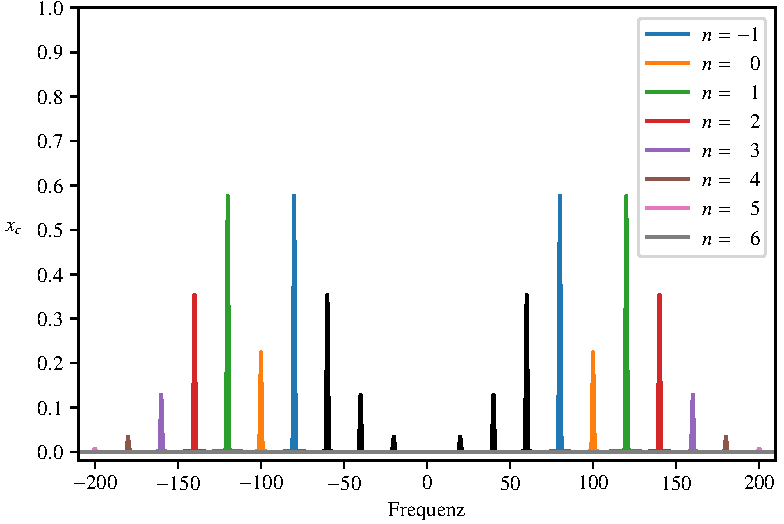
\includegraphics{papers/fm/images/beta2.pdf}
	%%% Creator: Matplotlib, PGF backend
%%
%% To include the figure in your LaTeX document, write
%%   \input{<filename>.pgf}
%%
%% Make sure the required packages are loaded in your preamble
%%   \usepackage{pgf}
%%
%% Also ensure that all the required font packages are loaded; for instance,
%% the lmodern package is sometimes necessary when using math font.
%%   \usepackage{lmodern}
%%
%% Figures using additional raster images can only be included by \input if
%% they are in the same directory as the main LaTeX file. For loading figures
%% from other directories you can use the `import` package
%%   \usepackage{import}
%%
%% and then include the figures with
%%   \import{<path to file>}{<filename>.pgf}
%%
%% Matplotlib used the following preamble
%%
\begingroup%
\makeatletter%
\begin{pgfpicture}%
\pgfpathrectangle{\pgfpointorigin}{\pgfqpoint{6.000000in}{4.000000in}}%
\pgfusepath{use as bounding box, clip}%
\begin{pgfscope}%
\pgfsetbuttcap%
\pgfsetmiterjoin%
\pgfsetlinewidth{0.000000pt}%
\definecolor{currentstroke}{rgb}{1.000000,1.000000,1.000000}%
\pgfsetstrokecolor{currentstroke}%
\pgfsetstrokeopacity{0.000000}%
\pgfsetdash{}{0pt}%
\pgfpathmoveto{\pgfqpoint{0.000000in}{0.000000in}}%
\pgfpathlineto{\pgfqpoint{6.000000in}{0.000000in}}%
\pgfpathlineto{\pgfqpoint{6.000000in}{4.000000in}}%
\pgfpathlineto{\pgfqpoint{0.000000in}{4.000000in}}%
\pgfpathlineto{\pgfqpoint{0.000000in}{0.000000in}}%
\pgfpathclose%
\pgfusepath{}%
\end{pgfscope}%
\begin{pgfscope}%
\pgfsetbuttcap%
\pgfsetmiterjoin%
\definecolor{currentfill}{rgb}{1.000000,1.000000,1.000000}%
\pgfsetfillcolor{currentfill}%
\pgfsetlinewidth{0.000000pt}%
\definecolor{currentstroke}{rgb}{0.000000,0.000000,0.000000}%
\pgfsetstrokecolor{currentstroke}%
\pgfsetstrokeopacity{0.000000}%
\pgfsetdash{}{0pt}%
\pgfpathmoveto{\pgfqpoint{0.750000in}{0.500000in}}%
\pgfpathlineto{\pgfqpoint{5.400000in}{0.500000in}}%
\pgfpathlineto{\pgfqpoint{5.400000in}{3.520000in}}%
\pgfpathlineto{\pgfqpoint{0.750000in}{3.520000in}}%
\pgfpathlineto{\pgfqpoint{0.750000in}{0.500000in}}%
\pgfpathclose%
\pgfusepath{fill}%
\end{pgfscope}%
\begin{pgfscope}%
\pgfsetbuttcap%
\pgfsetroundjoin%
\definecolor{currentfill}{rgb}{0.000000,0.000000,0.000000}%
\pgfsetfillcolor{currentfill}%
\pgfsetlinewidth{0.803000pt}%
\definecolor{currentstroke}{rgb}{0.000000,0.000000,0.000000}%
\pgfsetstrokecolor{currentstroke}%
\pgfsetdash{}{0pt}%
\pgfsys@defobject{currentmarker}{\pgfqpoint{0.000000in}{-0.048611in}}{\pgfqpoint{0.000000in}{0.000000in}}{%
\pgfpathmoveto{\pgfqpoint{0.000000in}{0.000000in}}%
\pgfpathlineto{\pgfqpoint{0.000000in}{-0.048611in}}%
\pgfusepath{stroke,fill}%
}%
\begin{pgfscope}%
\pgfsys@transformshift{0.860714in}{0.500000in}%
\pgfsys@useobject{currentmarker}{}%
\end{pgfscope}%
\end{pgfscope}%
\begin{pgfscope}%
\definecolor{textcolor}{rgb}{0.000000,0.000000,0.000000}%
\pgfsetstrokecolor{textcolor}%
\pgfsetfillcolor{textcolor}%
\pgftext[x=0.860714in,y=0.402778in,,top]{\color{textcolor}\rmfamily\fontsize{10.000000}{12.000000}\selectfont \(\displaystyle {\ensuremath{-}200}\)}%
\end{pgfscope}%
\begin{pgfscope}%
\pgfsetbuttcap%
\pgfsetroundjoin%
\definecolor{currentfill}{rgb}{0.000000,0.000000,0.000000}%
\pgfsetfillcolor{currentfill}%
\pgfsetlinewidth{0.803000pt}%
\definecolor{currentstroke}{rgb}{0.000000,0.000000,0.000000}%
\pgfsetstrokecolor{currentstroke}%
\pgfsetdash{}{0pt}%
\pgfsys@defobject{currentmarker}{\pgfqpoint{0.000000in}{-0.048611in}}{\pgfqpoint{0.000000in}{0.000000in}}{%
\pgfpathmoveto{\pgfqpoint{0.000000in}{0.000000in}}%
\pgfpathlineto{\pgfqpoint{0.000000in}{-0.048611in}}%
\pgfusepath{stroke,fill}%
}%
\begin{pgfscope}%
\pgfsys@transformshift{1.414286in}{0.500000in}%
\pgfsys@useobject{currentmarker}{}%
\end{pgfscope}%
\end{pgfscope}%
\begin{pgfscope}%
\definecolor{textcolor}{rgb}{0.000000,0.000000,0.000000}%
\pgfsetstrokecolor{textcolor}%
\pgfsetfillcolor{textcolor}%
\pgftext[x=1.414286in,y=0.402778in,,top]{\color{textcolor}\rmfamily\fontsize{10.000000}{12.000000}\selectfont \(\displaystyle {\ensuremath{-}150}\)}%
\end{pgfscope}%
\begin{pgfscope}%
\pgfsetbuttcap%
\pgfsetroundjoin%
\definecolor{currentfill}{rgb}{0.000000,0.000000,0.000000}%
\pgfsetfillcolor{currentfill}%
\pgfsetlinewidth{0.803000pt}%
\definecolor{currentstroke}{rgb}{0.000000,0.000000,0.000000}%
\pgfsetstrokecolor{currentstroke}%
\pgfsetdash{}{0pt}%
\pgfsys@defobject{currentmarker}{\pgfqpoint{0.000000in}{-0.048611in}}{\pgfqpoint{0.000000in}{0.000000in}}{%
\pgfpathmoveto{\pgfqpoint{0.000000in}{0.000000in}}%
\pgfpathlineto{\pgfqpoint{0.000000in}{-0.048611in}}%
\pgfusepath{stroke,fill}%
}%
\begin{pgfscope}%
\pgfsys@transformshift{1.967857in}{0.500000in}%
\pgfsys@useobject{currentmarker}{}%
\end{pgfscope}%
\end{pgfscope}%
\begin{pgfscope}%
\definecolor{textcolor}{rgb}{0.000000,0.000000,0.000000}%
\pgfsetstrokecolor{textcolor}%
\pgfsetfillcolor{textcolor}%
\pgftext[x=1.967857in,y=0.402778in,,top]{\color{textcolor}\rmfamily\fontsize{10.000000}{12.000000}\selectfont \(\displaystyle {\ensuremath{-}100}\)}%
\end{pgfscope}%
\begin{pgfscope}%
\pgfsetbuttcap%
\pgfsetroundjoin%
\definecolor{currentfill}{rgb}{0.000000,0.000000,0.000000}%
\pgfsetfillcolor{currentfill}%
\pgfsetlinewidth{0.803000pt}%
\definecolor{currentstroke}{rgb}{0.000000,0.000000,0.000000}%
\pgfsetstrokecolor{currentstroke}%
\pgfsetdash{}{0pt}%
\pgfsys@defobject{currentmarker}{\pgfqpoint{0.000000in}{-0.048611in}}{\pgfqpoint{0.000000in}{0.000000in}}{%
\pgfpathmoveto{\pgfqpoint{0.000000in}{0.000000in}}%
\pgfpathlineto{\pgfqpoint{0.000000in}{-0.048611in}}%
\pgfusepath{stroke,fill}%
}%
\begin{pgfscope}%
\pgfsys@transformshift{2.521429in}{0.500000in}%
\pgfsys@useobject{currentmarker}{}%
\end{pgfscope}%
\end{pgfscope}%
\begin{pgfscope}%
\definecolor{textcolor}{rgb}{0.000000,0.000000,0.000000}%
\pgfsetstrokecolor{textcolor}%
\pgfsetfillcolor{textcolor}%
\pgftext[x=2.521429in,y=0.402778in,,top]{\color{textcolor}\rmfamily\fontsize{10.000000}{12.000000}\selectfont \(\displaystyle {\ensuremath{-}50}\)}%
\end{pgfscope}%
\begin{pgfscope}%
\pgfsetbuttcap%
\pgfsetroundjoin%
\definecolor{currentfill}{rgb}{0.000000,0.000000,0.000000}%
\pgfsetfillcolor{currentfill}%
\pgfsetlinewidth{0.803000pt}%
\definecolor{currentstroke}{rgb}{0.000000,0.000000,0.000000}%
\pgfsetstrokecolor{currentstroke}%
\pgfsetdash{}{0pt}%
\pgfsys@defobject{currentmarker}{\pgfqpoint{0.000000in}{-0.048611in}}{\pgfqpoint{0.000000in}{0.000000in}}{%
\pgfpathmoveto{\pgfqpoint{0.000000in}{0.000000in}}%
\pgfpathlineto{\pgfqpoint{0.000000in}{-0.048611in}}%
\pgfusepath{stroke,fill}%
}%
\begin{pgfscope}%
\pgfsys@transformshift{3.075000in}{0.500000in}%
\pgfsys@useobject{currentmarker}{}%
\end{pgfscope}%
\end{pgfscope}%
\begin{pgfscope}%
\definecolor{textcolor}{rgb}{0.000000,0.000000,0.000000}%
\pgfsetstrokecolor{textcolor}%
\pgfsetfillcolor{textcolor}%
\pgftext[x=3.075000in,y=0.402778in,,top]{\color{textcolor}\rmfamily\fontsize{10.000000}{12.000000}\selectfont \(\displaystyle {0}\)}%
\end{pgfscope}%
\begin{pgfscope}%
\pgfsetbuttcap%
\pgfsetroundjoin%
\definecolor{currentfill}{rgb}{0.000000,0.000000,0.000000}%
\pgfsetfillcolor{currentfill}%
\pgfsetlinewidth{0.803000pt}%
\definecolor{currentstroke}{rgb}{0.000000,0.000000,0.000000}%
\pgfsetstrokecolor{currentstroke}%
\pgfsetdash{}{0pt}%
\pgfsys@defobject{currentmarker}{\pgfqpoint{0.000000in}{-0.048611in}}{\pgfqpoint{0.000000in}{0.000000in}}{%
\pgfpathmoveto{\pgfqpoint{0.000000in}{0.000000in}}%
\pgfpathlineto{\pgfqpoint{0.000000in}{-0.048611in}}%
\pgfusepath{stroke,fill}%
}%
\begin{pgfscope}%
\pgfsys@transformshift{3.628571in}{0.500000in}%
\pgfsys@useobject{currentmarker}{}%
\end{pgfscope}%
\end{pgfscope}%
\begin{pgfscope}%
\definecolor{textcolor}{rgb}{0.000000,0.000000,0.000000}%
\pgfsetstrokecolor{textcolor}%
\pgfsetfillcolor{textcolor}%
\pgftext[x=3.628571in,y=0.402778in,,top]{\color{textcolor}\rmfamily\fontsize{10.000000}{12.000000}\selectfont \(\displaystyle {50}\)}%
\end{pgfscope}%
\begin{pgfscope}%
\pgfsetbuttcap%
\pgfsetroundjoin%
\definecolor{currentfill}{rgb}{0.000000,0.000000,0.000000}%
\pgfsetfillcolor{currentfill}%
\pgfsetlinewidth{0.803000pt}%
\definecolor{currentstroke}{rgb}{0.000000,0.000000,0.000000}%
\pgfsetstrokecolor{currentstroke}%
\pgfsetdash{}{0pt}%
\pgfsys@defobject{currentmarker}{\pgfqpoint{0.000000in}{-0.048611in}}{\pgfqpoint{0.000000in}{0.000000in}}{%
\pgfpathmoveto{\pgfqpoint{0.000000in}{0.000000in}}%
\pgfpathlineto{\pgfqpoint{0.000000in}{-0.048611in}}%
\pgfusepath{stroke,fill}%
}%
\begin{pgfscope}%
\pgfsys@transformshift{4.182143in}{0.500000in}%
\pgfsys@useobject{currentmarker}{}%
\end{pgfscope}%
\end{pgfscope}%
\begin{pgfscope}%
\definecolor{textcolor}{rgb}{0.000000,0.000000,0.000000}%
\pgfsetstrokecolor{textcolor}%
\pgfsetfillcolor{textcolor}%
\pgftext[x=4.182143in,y=0.402778in,,top]{\color{textcolor}\rmfamily\fontsize{10.000000}{12.000000}\selectfont \(\displaystyle {100}\)}%
\end{pgfscope}%
\begin{pgfscope}%
\pgfsetbuttcap%
\pgfsetroundjoin%
\definecolor{currentfill}{rgb}{0.000000,0.000000,0.000000}%
\pgfsetfillcolor{currentfill}%
\pgfsetlinewidth{0.803000pt}%
\definecolor{currentstroke}{rgb}{0.000000,0.000000,0.000000}%
\pgfsetstrokecolor{currentstroke}%
\pgfsetdash{}{0pt}%
\pgfsys@defobject{currentmarker}{\pgfqpoint{0.000000in}{-0.048611in}}{\pgfqpoint{0.000000in}{0.000000in}}{%
\pgfpathmoveto{\pgfqpoint{0.000000in}{0.000000in}}%
\pgfpathlineto{\pgfqpoint{0.000000in}{-0.048611in}}%
\pgfusepath{stroke,fill}%
}%
\begin{pgfscope}%
\pgfsys@transformshift{4.735714in}{0.500000in}%
\pgfsys@useobject{currentmarker}{}%
\end{pgfscope}%
\end{pgfscope}%
\begin{pgfscope}%
\definecolor{textcolor}{rgb}{0.000000,0.000000,0.000000}%
\pgfsetstrokecolor{textcolor}%
\pgfsetfillcolor{textcolor}%
\pgftext[x=4.735714in,y=0.402778in,,top]{\color{textcolor}\rmfamily\fontsize{10.000000}{12.000000}\selectfont \(\displaystyle {150}\)}%
\end{pgfscope}%
\begin{pgfscope}%
\pgfsetbuttcap%
\pgfsetroundjoin%
\definecolor{currentfill}{rgb}{0.000000,0.000000,0.000000}%
\pgfsetfillcolor{currentfill}%
\pgfsetlinewidth{0.803000pt}%
\definecolor{currentstroke}{rgb}{0.000000,0.000000,0.000000}%
\pgfsetstrokecolor{currentstroke}%
\pgfsetdash{}{0pt}%
\pgfsys@defobject{currentmarker}{\pgfqpoint{0.000000in}{-0.048611in}}{\pgfqpoint{0.000000in}{0.000000in}}{%
\pgfpathmoveto{\pgfqpoint{0.000000in}{0.000000in}}%
\pgfpathlineto{\pgfqpoint{0.000000in}{-0.048611in}}%
\pgfusepath{stroke,fill}%
}%
\begin{pgfscope}%
\pgfsys@transformshift{5.289286in}{0.500000in}%
\pgfsys@useobject{currentmarker}{}%
\end{pgfscope}%
\end{pgfscope}%
\begin{pgfscope}%
\definecolor{textcolor}{rgb}{0.000000,0.000000,0.000000}%
\pgfsetstrokecolor{textcolor}%
\pgfsetfillcolor{textcolor}%
\pgftext[x=5.289286in,y=0.402778in,,top]{\color{textcolor}\rmfamily\fontsize{10.000000}{12.000000}\selectfont \(\displaystyle {200}\)}%
\end{pgfscope}%
\begin{pgfscope}%
\definecolor{textcolor}{rgb}{0.000000,0.000000,0.000000}%
\pgfsetstrokecolor{textcolor}%
\pgfsetfillcolor{textcolor}%
\pgftext[x=3.075000in,y=0.223766in,,top]{\color{textcolor}\rmfamily\fontsize{10.000000}{12.000000}\selectfont Frequency}%
\end{pgfscope}%
\begin{pgfscope}%
\pgfsetbuttcap%
\pgfsetroundjoin%
\definecolor{currentfill}{rgb}{0.000000,0.000000,0.000000}%
\pgfsetfillcolor{currentfill}%
\pgfsetlinewidth{0.803000pt}%
\definecolor{currentstroke}{rgb}{0.000000,0.000000,0.000000}%
\pgfsetstrokecolor{currentstroke}%
\pgfsetdash{}{0pt}%
\pgfsys@defobject{currentmarker}{\pgfqpoint{-0.048611in}{0.000000in}}{\pgfqpoint{-0.000000in}{0.000000in}}{%
\pgfpathmoveto{\pgfqpoint{-0.000000in}{0.000000in}}%
\pgfpathlineto{\pgfqpoint{-0.048611in}{0.000000in}}%
\pgfusepath{stroke,fill}%
}%
\begin{pgfscope}%
\pgfsys@transformshift{0.750000in}{0.559216in}%
\pgfsys@useobject{currentmarker}{}%
\end{pgfscope}%
\end{pgfscope}%
\begin{pgfscope}%
\definecolor{textcolor}{rgb}{0.000000,0.000000,0.000000}%
\pgfsetstrokecolor{textcolor}%
\pgfsetfillcolor{textcolor}%
\pgftext[x=0.475308in, y=0.510990in, left, base]{\color{textcolor}\rmfamily\fontsize{10.000000}{12.000000}\selectfont \(\displaystyle {0.0}\)}%
\end{pgfscope}%
\begin{pgfscope}%
\pgfsetbuttcap%
\pgfsetroundjoin%
\definecolor{currentfill}{rgb}{0.000000,0.000000,0.000000}%
\pgfsetfillcolor{currentfill}%
\pgfsetlinewidth{0.803000pt}%
\definecolor{currentstroke}{rgb}{0.000000,0.000000,0.000000}%
\pgfsetstrokecolor{currentstroke}%
\pgfsetdash{}{0pt}%
\pgfsys@defobject{currentmarker}{\pgfqpoint{-0.048611in}{0.000000in}}{\pgfqpoint{-0.000000in}{0.000000in}}{%
\pgfpathmoveto{\pgfqpoint{-0.000000in}{0.000000in}}%
\pgfpathlineto{\pgfqpoint{-0.048611in}{0.000000in}}%
\pgfusepath{stroke,fill}%
}%
\begin{pgfscope}%
\pgfsys@transformshift{0.750000in}{0.855294in}%
\pgfsys@useobject{currentmarker}{}%
\end{pgfscope}%
\end{pgfscope}%
\begin{pgfscope}%
\definecolor{textcolor}{rgb}{0.000000,0.000000,0.000000}%
\pgfsetstrokecolor{textcolor}%
\pgfsetfillcolor{textcolor}%
\pgftext[x=0.475308in, y=0.807069in, left, base]{\color{textcolor}\rmfamily\fontsize{10.000000}{12.000000}\selectfont \(\displaystyle {0.1}\)}%
\end{pgfscope}%
\begin{pgfscope}%
\pgfsetbuttcap%
\pgfsetroundjoin%
\definecolor{currentfill}{rgb}{0.000000,0.000000,0.000000}%
\pgfsetfillcolor{currentfill}%
\pgfsetlinewidth{0.803000pt}%
\definecolor{currentstroke}{rgb}{0.000000,0.000000,0.000000}%
\pgfsetstrokecolor{currentstroke}%
\pgfsetdash{}{0pt}%
\pgfsys@defobject{currentmarker}{\pgfqpoint{-0.048611in}{0.000000in}}{\pgfqpoint{-0.000000in}{0.000000in}}{%
\pgfpathmoveto{\pgfqpoint{-0.000000in}{0.000000in}}%
\pgfpathlineto{\pgfqpoint{-0.048611in}{0.000000in}}%
\pgfusepath{stroke,fill}%
}%
\begin{pgfscope}%
\pgfsys@transformshift{0.750000in}{1.151373in}%
\pgfsys@useobject{currentmarker}{}%
\end{pgfscope}%
\end{pgfscope}%
\begin{pgfscope}%
\definecolor{textcolor}{rgb}{0.000000,0.000000,0.000000}%
\pgfsetstrokecolor{textcolor}%
\pgfsetfillcolor{textcolor}%
\pgftext[x=0.475308in, y=1.103147in, left, base]{\color{textcolor}\rmfamily\fontsize{10.000000}{12.000000}\selectfont \(\displaystyle {0.2}\)}%
\end{pgfscope}%
\begin{pgfscope}%
\pgfsetbuttcap%
\pgfsetroundjoin%
\definecolor{currentfill}{rgb}{0.000000,0.000000,0.000000}%
\pgfsetfillcolor{currentfill}%
\pgfsetlinewidth{0.803000pt}%
\definecolor{currentstroke}{rgb}{0.000000,0.000000,0.000000}%
\pgfsetstrokecolor{currentstroke}%
\pgfsetdash{}{0pt}%
\pgfsys@defobject{currentmarker}{\pgfqpoint{-0.048611in}{0.000000in}}{\pgfqpoint{-0.000000in}{0.000000in}}{%
\pgfpathmoveto{\pgfqpoint{-0.000000in}{0.000000in}}%
\pgfpathlineto{\pgfqpoint{-0.048611in}{0.000000in}}%
\pgfusepath{stroke,fill}%
}%
\begin{pgfscope}%
\pgfsys@transformshift{0.750000in}{1.447451in}%
\pgfsys@useobject{currentmarker}{}%
\end{pgfscope}%
\end{pgfscope}%
\begin{pgfscope}%
\definecolor{textcolor}{rgb}{0.000000,0.000000,0.000000}%
\pgfsetstrokecolor{textcolor}%
\pgfsetfillcolor{textcolor}%
\pgftext[x=0.475308in, y=1.399226in, left, base]{\color{textcolor}\rmfamily\fontsize{10.000000}{12.000000}\selectfont \(\displaystyle {0.3}\)}%
\end{pgfscope}%
\begin{pgfscope}%
\pgfsetbuttcap%
\pgfsetroundjoin%
\definecolor{currentfill}{rgb}{0.000000,0.000000,0.000000}%
\pgfsetfillcolor{currentfill}%
\pgfsetlinewidth{0.803000pt}%
\definecolor{currentstroke}{rgb}{0.000000,0.000000,0.000000}%
\pgfsetstrokecolor{currentstroke}%
\pgfsetdash{}{0pt}%
\pgfsys@defobject{currentmarker}{\pgfqpoint{-0.048611in}{0.000000in}}{\pgfqpoint{-0.000000in}{0.000000in}}{%
\pgfpathmoveto{\pgfqpoint{-0.000000in}{0.000000in}}%
\pgfpathlineto{\pgfqpoint{-0.048611in}{0.000000in}}%
\pgfusepath{stroke,fill}%
}%
\begin{pgfscope}%
\pgfsys@transformshift{0.750000in}{1.743529in}%
\pgfsys@useobject{currentmarker}{}%
\end{pgfscope}%
\end{pgfscope}%
\begin{pgfscope}%
\definecolor{textcolor}{rgb}{0.000000,0.000000,0.000000}%
\pgfsetstrokecolor{textcolor}%
\pgfsetfillcolor{textcolor}%
\pgftext[x=0.475308in, y=1.695304in, left, base]{\color{textcolor}\rmfamily\fontsize{10.000000}{12.000000}\selectfont \(\displaystyle {0.4}\)}%
\end{pgfscope}%
\begin{pgfscope}%
\pgfsetbuttcap%
\pgfsetroundjoin%
\definecolor{currentfill}{rgb}{0.000000,0.000000,0.000000}%
\pgfsetfillcolor{currentfill}%
\pgfsetlinewidth{0.803000pt}%
\definecolor{currentstroke}{rgb}{0.000000,0.000000,0.000000}%
\pgfsetstrokecolor{currentstroke}%
\pgfsetdash{}{0pt}%
\pgfsys@defobject{currentmarker}{\pgfqpoint{-0.048611in}{0.000000in}}{\pgfqpoint{-0.000000in}{0.000000in}}{%
\pgfpathmoveto{\pgfqpoint{-0.000000in}{0.000000in}}%
\pgfpathlineto{\pgfqpoint{-0.048611in}{0.000000in}}%
\pgfusepath{stroke,fill}%
}%
\begin{pgfscope}%
\pgfsys@transformshift{0.750000in}{2.039608in}%
\pgfsys@useobject{currentmarker}{}%
\end{pgfscope}%
\end{pgfscope}%
\begin{pgfscope}%
\definecolor{textcolor}{rgb}{0.000000,0.000000,0.000000}%
\pgfsetstrokecolor{textcolor}%
\pgfsetfillcolor{textcolor}%
\pgftext[x=0.475308in, y=1.991383in, left, base]{\color{textcolor}\rmfamily\fontsize{10.000000}{12.000000}\selectfont \(\displaystyle {0.5}\)}%
\end{pgfscope}%
\begin{pgfscope}%
\pgfsetbuttcap%
\pgfsetroundjoin%
\definecolor{currentfill}{rgb}{0.000000,0.000000,0.000000}%
\pgfsetfillcolor{currentfill}%
\pgfsetlinewidth{0.803000pt}%
\definecolor{currentstroke}{rgb}{0.000000,0.000000,0.000000}%
\pgfsetstrokecolor{currentstroke}%
\pgfsetdash{}{0pt}%
\pgfsys@defobject{currentmarker}{\pgfqpoint{-0.048611in}{0.000000in}}{\pgfqpoint{-0.000000in}{0.000000in}}{%
\pgfpathmoveto{\pgfqpoint{-0.000000in}{0.000000in}}%
\pgfpathlineto{\pgfqpoint{-0.048611in}{0.000000in}}%
\pgfusepath{stroke,fill}%
}%
\begin{pgfscope}%
\pgfsys@transformshift{0.750000in}{2.335686in}%
\pgfsys@useobject{currentmarker}{}%
\end{pgfscope}%
\end{pgfscope}%
\begin{pgfscope}%
\definecolor{textcolor}{rgb}{0.000000,0.000000,0.000000}%
\pgfsetstrokecolor{textcolor}%
\pgfsetfillcolor{textcolor}%
\pgftext[x=0.475308in, y=2.287461in, left, base]{\color{textcolor}\rmfamily\fontsize{10.000000}{12.000000}\selectfont \(\displaystyle {0.6}\)}%
\end{pgfscope}%
\begin{pgfscope}%
\pgfsetbuttcap%
\pgfsetroundjoin%
\definecolor{currentfill}{rgb}{0.000000,0.000000,0.000000}%
\pgfsetfillcolor{currentfill}%
\pgfsetlinewidth{0.803000pt}%
\definecolor{currentstroke}{rgb}{0.000000,0.000000,0.000000}%
\pgfsetstrokecolor{currentstroke}%
\pgfsetdash{}{0pt}%
\pgfsys@defobject{currentmarker}{\pgfqpoint{-0.048611in}{0.000000in}}{\pgfqpoint{-0.000000in}{0.000000in}}{%
\pgfpathmoveto{\pgfqpoint{-0.000000in}{0.000000in}}%
\pgfpathlineto{\pgfqpoint{-0.048611in}{0.000000in}}%
\pgfusepath{stroke,fill}%
}%
\begin{pgfscope}%
\pgfsys@transformshift{0.750000in}{2.631765in}%
\pgfsys@useobject{currentmarker}{}%
\end{pgfscope}%
\end{pgfscope}%
\begin{pgfscope}%
\definecolor{textcolor}{rgb}{0.000000,0.000000,0.000000}%
\pgfsetstrokecolor{textcolor}%
\pgfsetfillcolor{textcolor}%
\pgftext[x=0.475308in, y=2.583539in, left, base]{\color{textcolor}\rmfamily\fontsize{10.000000}{12.000000}\selectfont \(\displaystyle {0.7}\)}%
\end{pgfscope}%
\begin{pgfscope}%
\pgfsetbuttcap%
\pgfsetroundjoin%
\definecolor{currentfill}{rgb}{0.000000,0.000000,0.000000}%
\pgfsetfillcolor{currentfill}%
\pgfsetlinewidth{0.803000pt}%
\definecolor{currentstroke}{rgb}{0.000000,0.000000,0.000000}%
\pgfsetstrokecolor{currentstroke}%
\pgfsetdash{}{0pt}%
\pgfsys@defobject{currentmarker}{\pgfqpoint{-0.048611in}{0.000000in}}{\pgfqpoint{-0.000000in}{0.000000in}}{%
\pgfpathmoveto{\pgfqpoint{-0.000000in}{0.000000in}}%
\pgfpathlineto{\pgfqpoint{-0.048611in}{0.000000in}}%
\pgfusepath{stroke,fill}%
}%
\begin{pgfscope}%
\pgfsys@transformshift{0.750000in}{2.927843in}%
\pgfsys@useobject{currentmarker}{}%
\end{pgfscope}%
\end{pgfscope}%
\begin{pgfscope}%
\definecolor{textcolor}{rgb}{0.000000,0.000000,0.000000}%
\pgfsetstrokecolor{textcolor}%
\pgfsetfillcolor{textcolor}%
\pgftext[x=0.475308in, y=2.879618in, left, base]{\color{textcolor}\rmfamily\fontsize{10.000000}{12.000000}\selectfont \(\displaystyle {0.8}\)}%
\end{pgfscope}%
\begin{pgfscope}%
\pgfsetbuttcap%
\pgfsetroundjoin%
\definecolor{currentfill}{rgb}{0.000000,0.000000,0.000000}%
\pgfsetfillcolor{currentfill}%
\pgfsetlinewidth{0.803000pt}%
\definecolor{currentstroke}{rgb}{0.000000,0.000000,0.000000}%
\pgfsetstrokecolor{currentstroke}%
\pgfsetdash{}{0pt}%
\pgfsys@defobject{currentmarker}{\pgfqpoint{-0.048611in}{0.000000in}}{\pgfqpoint{-0.000000in}{0.000000in}}{%
\pgfpathmoveto{\pgfqpoint{-0.000000in}{0.000000in}}%
\pgfpathlineto{\pgfqpoint{-0.048611in}{0.000000in}}%
\pgfusepath{stroke,fill}%
}%
\begin{pgfscope}%
\pgfsys@transformshift{0.750000in}{3.223922in}%
\pgfsys@useobject{currentmarker}{}%
\end{pgfscope}%
\end{pgfscope}%
\begin{pgfscope}%
\definecolor{textcolor}{rgb}{0.000000,0.000000,0.000000}%
\pgfsetstrokecolor{textcolor}%
\pgfsetfillcolor{textcolor}%
\pgftext[x=0.475308in, y=3.175696in, left, base]{\color{textcolor}\rmfamily\fontsize{10.000000}{12.000000}\selectfont \(\displaystyle {0.9}\)}%
\end{pgfscope}%
\begin{pgfscope}%
\pgfsetbuttcap%
\pgfsetroundjoin%
\definecolor{currentfill}{rgb}{0.000000,0.000000,0.000000}%
\pgfsetfillcolor{currentfill}%
\pgfsetlinewidth{0.803000pt}%
\definecolor{currentstroke}{rgb}{0.000000,0.000000,0.000000}%
\pgfsetstrokecolor{currentstroke}%
\pgfsetdash{}{0pt}%
\pgfsys@defobject{currentmarker}{\pgfqpoint{-0.048611in}{0.000000in}}{\pgfqpoint{-0.000000in}{0.000000in}}{%
\pgfpathmoveto{\pgfqpoint{-0.000000in}{0.000000in}}%
\pgfpathlineto{\pgfqpoint{-0.048611in}{0.000000in}}%
\pgfusepath{stroke,fill}%
}%
\begin{pgfscope}%
\pgfsys@transformshift{0.750000in}{3.520000in}%
\pgfsys@useobject{currentmarker}{}%
\end{pgfscope}%
\end{pgfscope}%
\begin{pgfscope}%
\definecolor{textcolor}{rgb}{0.000000,0.000000,0.000000}%
\pgfsetstrokecolor{textcolor}%
\pgfsetfillcolor{textcolor}%
\pgftext[x=0.475308in, y=3.471775in, left, base]{\color{textcolor}\rmfamily\fontsize{10.000000}{12.000000}\selectfont \(\displaystyle {1.0}\)}%
\end{pgfscope}%
\begin{pgfscope}%
\definecolor{textcolor}{rgb}{0.000000,0.000000,0.000000}%
\pgfsetstrokecolor{textcolor}%
\pgfsetfillcolor{textcolor}%
\pgftext[x=0.419753in,y=2.010000in,,bottom,rotate=90.000000]{\color{textcolor}\rmfamily\fontsize{10.000000}{12.000000}\selectfont \(\displaystyle x_c\)}%
\end{pgfscope}%
\begin{pgfscope}%
\pgfpathrectangle{\pgfqpoint{0.750000in}{0.500000in}}{\pgfqpoint{4.650000in}{3.020000in}}%
\pgfusepath{clip}%
\pgfsetrectcap%
\pgfsetroundjoin%
\pgfsetlinewidth{1.505625pt}%
\definecolor{currentstroke}{rgb}{0.000000,0.000000,0.000000}%
\pgfsetstrokecolor{currentstroke}%
\pgfsetdash{}{0pt}%
\pgfpathmoveto{\pgfqpoint{3.075000in}{0.559216in}}%
\pgfpathlineto{\pgfqpoint{3.285357in}{0.559223in}}%
\pgfpathlineto{\pgfqpoint{3.296429in}{0.562776in}}%
\pgfpathlineto{\pgfqpoint{3.307500in}{0.559223in}}%
\pgfpathlineto{\pgfqpoint{5.413889in}{0.559216in}}%
\pgfpathmoveto{\pgfqpoint{5.413889in}{0.559216in}}%
\pgfpathlineto{\pgfqpoint{0.736111in}{0.559216in}}%
\pgfpathmoveto{\pgfqpoint{0.736111in}{0.559216in}}%
\pgfpathlineto{\pgfqpoint{2.842500in}{0.559223in}}%
\pgfpathlineto{\pgfqpoint{2.853571in}{0.562776in}}%
\pgfpathlineto{\pgfqpoint{2.864643in}{0.559223in}}%
\pgfpathlineto{\pgfqpoint{3.063929in}{0.559216in}}%
\pgfpathlineto{\pgfqpoint{3.063929in}{0.559216in}}%
\pgfusepath{stroke}%
\end{pgfscope}%
\begin{pgfscope}%
\pgfpathrectangle{\pgfqpoint{0.750000in}{0.500000in}}{\pgfqpoint{4.650000in}{3.020000in}}%
\pgfusepath{clip}%
\pgfsetrectcap%
\pgfsetroundjoin%
\pgfsetlinewidth{1.505625pt}%
\definecolor{currentstroke}{rgb}{0.000000,0.000000,0.000000}%
\pgfsetstrokecolor{currentstroke}%
\pgfsetdash{}{0pt}%
\pgfpathmoveto{\pgfqpoint{3.075000in}{0.559216in}}%
\pgfpathlineto{\pgfqpoint{5.413889in}{0.559216in}}%
\pgfpathmoveto{\pgfqpoint{5.413889in}{0.559216in}}%
\pgfpathlineto{\pgfqpoint{0.736111in}{0.559216in}}%
\pgfpathmoveto{\pgfqpoint{0.736111in}{0.559216in}}%
\pgfpathlineto{\pgfqpoint{3.063929in}{0.559216in}}%
\pgfpathlineto{\pgfqpoint{3.063929in}{0.559216in}}%
\pgfusepath{stroke}%
\end{pgfscope}%
\begin{pgfscope}%
\pgfpathrectangle{\pgfqpoint{0.750000in}{0.500000in}}{\pgfqpoint{4.650000in}{3.020000in}}%
\pgfusepath{clip}%
\pgfsetrectcap%
\pgfsetroundjoin%
\pgfsetlinewidth{1.505625pt}%
\definecolor{currentstroke}{rgb}{0.000000,0.000000,0.000000}%
\pgfsetstrokecolor{currentstroke}%
\pgfsetdash{}{0pt}%
\pgfpathmoveto{\pgfqpoint{3.075000in}{0.559235in}}%
\pgfpathlineto{\pgfqpoint{3.285357in}{0.559421in}}%
\pgfpathlineto{\pgfqpoint{3.296429in}{0.659873in}}%
\pgfpathlineto{\pgfqpoint{3.307500in}{0.559413in}}%
\pgfpathlineto{\pgfqpoint{3.495714in}{0.559224in}}%
\pgfpathlineto{\pgfqpoint{5.413889in}{0.559216in}}%
\pgfpathmoveto{\pgfqpoint{5.413889in}{0.559216in}}%
\pgfpathlineto{\pgfqpoint{0.736111in}{0.559216in}}%
\pgfpathmoveto{\pgfqpoint{0.736111in}{0.559216in}}%
\pgfpathlineto{\pgfqpoint{2.842500in}{0.559413in}}%
\pgfpathlineto{\pgfqpoint{2.853571in}{0.659873in}}%
\pgfpathlineto{\pgfqpoint{2.864643in}{0.559421in}}%
\pgfpathlineto{\pgfqpoint{3.052857in}{0.559235in}}%
\pgfpathlineto{\pgfqpoint{3.063929in}{0.559235in}}%
\pgfpathlineto{\pgfqpoint{3.063929in}{0.559235in}}%
\pgfusepath{stroke}%
\end{pgfscope}%
\begin{pgfscope}%
\pgfpathrectangle{\pgfqpoint{0.750000in}{0.500000in}}{\pgfqpoint{4.650000in}{3.020000in}}%
\pgfusepath{clip}%
\pgfsetrectcap%
\pgfsetroundjoin%
\pgfsetlinewidth{1.505625pt}%
\definecolor{currentstroke}{rgb}{0.000000,0.000000,0.000000}%
\pgfsetstrokecolor{currentstroke}%
\pgfsetdash{}{0pt}%
\pgfpathmoveto{\pgfqpoint{3.075000in}{0.559261in}}%
\pgfpathlineto{\pgfqpoint{3.506786in}{0.560731in}}%
\pgfpathlineto{\pgfqpoint{3.517857in}{0.940973in}}%
\pgfpathlineto{\pgfqpoint{3.528929in}{0.560755in}}%
\pgfpathlineto{\pgfqpoint{3.562143in}{0.559604in}}%
\pgfpathlineto{\pgfqpoint{3.827857in}{0.559276in}}%
\pgfpathlineto{\pgfqpoint{5.413889in}{0.559228in}}%
\pgfpathmoveto{\pgfqpoint{5.413889in}{0.559216in}}%
\pgfpathlineto{\pgfqpoint{0.736111in}{0.559216in}}%
\pgfpathmoveto{\pgfqpoint{0.736111in}{0.559228in}}%
\pgfpathlineto{\pgfqpoint{2.621071in}{0.560755in}}%
\pgfpathlineto{\pgfqpoint{2.632143in}{0.940973in}}%
\pgfpathlineto{\pgfqpoint{2.643214in}{0.560731in}}%
\pgfpathlineto{\pgfqpoint{2.676429in}{0.559591in}}%
\pgfpathlineto{\pgfqpoint{2.942143in}{0.559269in}}%
\pgfpathlineto{\pgfqpoint{3.063929in}{0.559261in}}%
\pgfpathlineto{\pgfqpoint{3.063929in}{0.559261in}}%
\pgfusepath{stroke}%
\end{pgfscope}%
\begin{pgfscope}%
\pgfpathrectangle{\pgfqpoint{0.750000in}{0.500000in}}{\pgfqpoint{4.650000in}{3.020000in}}%
\pgfusepath{clip}%
\pgfsetrectcap%
\pgfsetroundjoin%
\pgfsetlinewidth{1.505625pt}%
\definecolor{currentstroke}{rgb}{0.000000,0.000000,0.000000}%
\pgfsetstrokecolor{currentstroke}%
\pgfsetdash{}{0pt}%
\pgfpathmoveto{\pgfqpoint{3.075000in}{0.559338in}}%
\pgfpathlineto{\pgfqpoint{3.695000in}{0.560765in}}%
\pgfpathlineto{\pgfqpoint{3.717143in}{0.562324in}}%
\pgfpathlineto{\pgfqpoint{3.728214in}{0.565430in}}%
\pgfpathlineto{\pgfqpoint{3.739286in}{1.603803in}}%
\pgfpathlineto{\pgfqpoint{3.750357in}{0.565538in}}%
\pgfpathlineto{\pgfqpoint{3.761429in}{0.562376in}}%
\pgfpathlineto{\pgfqpoint{3.794643in}{0.560487in}}%
\pgfpathlineto{\pgfqpoint{3.916429in}{0.559624in}}%
\pgfpathlineto{\pgfqpoint{4.813214in}{0.559294in}}%
\pgfpathlineto{\pgfqpoint{5.413889in}{0.559269in}}%
\pgfpathmoveto{\pgfqpoint{5.413889in}{0.559219in}}%
\pgfpathlineto{\pgfqpoint{0.736111in}{0.559219in}}%
\pgfpathmoveto{\pgfqpoint{0.736111in}{0.559269in}}%
\pgfpathlineto{\pgfqpoint{2.366429in}{0.560801in}}%
\pgfpathlineto{\pgfqpoint{2.388571in}{0.562376in}}%
\pgfpathlineto{\pgfqpoint{2.399643in}{0.565538in}}%
\pgfpathlineto{\pgfqpoint{2.410714in}{1.603803in}}%
\pgfpathlineto{\pgfqpoint{2.421786in}{0.565430in}}%
\pgfpathlineto{\pgfqpoint{2.432857in}{0.562324in}}%
\pgfpathlineto{\pgfqpoint{2.466071in}{0.560452in}}%
\pgfpathlineto{\pgfqpoint{2.587857in}{0.559593in}}%
\pgfpathlineto{\pgfqpoint{3.063929in}{0.559339in}}%
\pgfpathlineto{\pgfqpoint{3.063929in}{0.559339in}}%
\pgfusepath{stroke}%
\end{pgfscope}%
\begin{pgfscope}%
\pgfpathrectangle{\pgfqpoint{0.750000in}{0.500000in}}{\pgfqpoint{4.650000in}{3.020000in}}%
\pgfusepath{clip}%
\pgfsetrectcap%
\pgfsetroundjoin%
\pgfsetlinewidth{1.505625pt}%
\definecolor{currentstroke}{rgb}{0.121569,0.466667,0.705882}%
\pgfsetstrokecolor{currentstroke}%
\pgfsetdash{}{0pt}%
\pgfpathmoveto{\pgfqpoint{3.075000in}{0.559540in}}%
\pgfpathlineto{\pgfqpoint{3.872143in}{0.560995in}}%
\pgfpathlineto{\pgfqpoint{3.916429in}{0.562695in}}%
\pgfpathlineto{\pgfqpoint{3.938571in}{0.566089in}}%
\pgfpathlineto{\pgfqpoint{3.949643in}{0.572837in}}%
\pgfpathlineto{\pgfqpoint{3.960714in}{2.266663in}}%
\pgfpathlineto{\pgfqpoint{3.971786in}{0.572918in}}%
\pgfpathlineto{\pgfqpoint{3.982857in}{0.566005in}}%
\pgfpathlineto{\pgfqpoint{4.005000in}{0.562571in}}%
\pgfpathlineto{\pgfqpoint{4.060357in}{0.560670in}}%
\pgfpathlineto{\pgfqpoint{4.237500in}{0.559704in}}%
\pgfpathlineto{\pgfqpoint{5.278214in}{0.559296in}}%
\pgfpathlineto{\pgfqpoint{5.413889in}{0.559287in}}%
\pgfpathmoveto{\pgfqpoint{5.413889in}{0.559218in}}%
\pgfpathlineto{\pgfqpoint{0.736111in}{0.559218in}}%
\pgfpathmoveto{\pgfqpoint{0.736111in}{0.559287in}}%
\pgfpathlineto{\pgfqpoint{2.100714in}{0.560860in}}%
\pgfpathlineto{\pgfqpoint{2.145000in}{0.562571in}}%
\pgfpathlineto{\pgfqpoint{2.167143in}{0.566005in}}%
\pgfpathlineto{\pgfqpoint{2.178214in}{0.572918in}}%
\pgfpathlineto{\pgfqpoint{2.189286in}{2.266663in}}%
\pgfpathlineto{\pgfqpoint{2.200357in}{0.572837in}}%
\pgfpathlineto{\pgfqpoint{2.211429in}{0.566089in}}%
\pgfpathlineto{\pgfqpoint{2.233571in}{0.562695in}}%
\pgfpathlineto{\pgfqpoint{2.288929in}{0.560806in}}%
\pgfpathlineto{\pgfqpoint{2.466071in}{0.559847in}}%
\pgfpathlineto{\pgfqpoint{3.063929in}{0.559541in}}%
\pgfpathlineto{\pgfqpoint{3.063929in}{0.559541in}}%
\pgfusepath{stroke}%
\end{pgfscope}%
\begin{pgfscope}%
\pgfpathrectangle{\pgfqpoint{0.750000in}{0.500000in}}{\pgfqpoint{4.650000in}{3.020000in}}%
\pgfusepath{clip}%
\pgfsetrectcap%
\pgfsetroundjoin%
\pgfsetlinewidth{1.505625pt}%
\definecolor{currentstroke}{rgb}{1.000000,0.498039,0.054902}%
\pgfsetstrokecolor{currentstroke}%
\pgfsetdash{}{0pt}%
\pgfpathmoveto{\pgfqpoint{3.075000in}{0.559216in}}%
\pgfpathlineto{\pgfqpoint{4.137857in}{0.560835in}}%
\pgfpathlineto{\pgfqpoint{4.160000in}{0.562480in}}%
\pgfpathlineto{\pgfqpoint{4.171071in}{0.565745in}}%
\pgfpathlineto{\pgfqpoint{4.182143in}{1.221966in}}%
\pgfpathlineto{\pgfqpoint{4.193214in}{0.565944in}}%
\pgfpathlineto{\pgfqpoint{4.204286in}{0.562579in}}%
\pgfpathlineto{\pgfqpoint{4.237500in}{0.560576in}}%
\pgfpathlineto{\pgfqpoint{4.359286in}{0.559661in}}%
\pgfpathlineto{\pgfqpoint{5.211786in}{0.559310in}}%
\pgfpathlineto{\pgfqpoint{5.413889in}{0.559297in}}%
\pgfpathmoveto{\pgfqpoint{5.413889in}{0.559220in}}%
\pgfpathlineto{\pgfqpoint{0.736111in}{0.559220in}}%
\pgfpathmoveto{\pgfqpoint{0.736111in}{0.559297in}}%
\pgfpathlineto{\pgfqpoint{1.912500in}{0.560576in}}%
\pgfpathlineto{\pgfqpoint{1.945714in}{0.562579in}}%
\pgfpathlineto{\pgfqpoint{1.956786in}{0.565944in}}%
\pgfpathlineto{\pgfqpoint{1.967857in}{1.221966in}}%
\pgfpathlineto{\pgfqpoint{1.978929in}{0.565745in}}%
\pgfpathlineto{\pgfqpoint{1.990000in}{0.562480in}}%
\pgfpathlineto{\pgfqpoint{2.023214in}{0.560505in}}%
\pgfpathlineto{\pgfqpoint{2.145000in}{0.559594in}}%
\pgfpathlineto{\pgfqpoint{2.997500in}{0.559225in}}%
\pgfpathlineto{\pgfqpoint{3.063929in}{0.559217in}}%
\pgfpathlineto{\pgfqpoint{3.063929in}{0.559217in}}%
\pgfusepath{stroke}%
\end{pgfscope}%
\begin{pgfscope}%
\pgfpathrectangle{\pgfqpoint{0.750000in}{0.500000in}}{\pgfqpoint{4.650000in}{3.020000in}}%
\pgfusepath{clip}%
\pgfsetrectcap%
\pgfsetroundjoin%
\pgfsetlinewidth{1.505625pt}%
\definecolor{currentstroke}{rgb}{0.172549,0.627451,0.172549}%
\pgfsetstrokecolor{currentstroke}%
\pgfsetdash{}{0pt}%
\pgfpathmoveto{\pgfqpoint{3.075000in}{0.559540in}}%
\pgfpathlineto{\pgfqpoint{4.270714in}{0.560995in}}%
\pgfpathlineto{\pgfqpoint{4.348214in}{0.563374in}}%
\pgfpathlineto{\pgfqpoint{4.370357in}{0.566088in}}%
\pgfpathlineto{\pgfqpoint{4.381429in}{0.569468in}}%
\pgfpathlineto{\pgfqpoint{4.392500in}{0.579530in}}%
\pgfpathlineto{\pgfqpoint{4.403571in}{2.266438in}}%
\pgfpathlineto{\pgfqpoint{4.414643in}{0.579884in}}%
\pgfpathlineto{\pgfqpoint{4.425714in}{0.569453in}}%
\pgfpathlineto{\pgfqpoint{4.436786in}{0.566004in}}%
\pgfpathlineto{\pgfqpoint{4.458929in}{0.563256in}}%
\pgfpathlineto{\pgfqpoint{4.514286in}{0.561201in}}%
\pgfpathlineto{\pgfqpoint{4.669286in}{0.560008in}}%
\pgfpathlineto{\pgfqpoint{5.366786in}{0.559404in}}%
\pgfpathlineto{\pgfqpoint{5.413889in}{0.559394in}}%
\pgfpathmoveto{\pgfqpoint{5.413889in}{0.559220in}}%
\pgfpathlineto{\pgfqpoint{0.736111in}{0.559220in}}%
\pgfpathmoveto{\pgfqpoint{0.736111in}{0.559394in}}%
\pgfpathlineto{\pgfqpoint{1.624643in}{0.561015in}}%
\pgfpathlineto{\pgfqpoint{1.691071in}{0.563256in}}%
\pgfpathlineto{\pgfqpoint{1.713214in}{0.566004in}}%
\pgfpathlineto{\pgfqpoint{1.724286in}{0.569453in}}%
\pgfpathlineto{\pgfqpoint{1.735357in}{0.579884in}}%
\pgfpathlineto{\pgfqpoint{1.746429in}{2.266438in}}%
\pgfpathlineto{\pgfqpoint{1.757500in}{0.579530in}}%
\pgfpathlineto{\pgfqpoint{1.768571in}{0.569468in}}%
\pgfpathlineto{\pgfqpoint{1.779643in}{0.566088in}}%
\pgfpathlineto{\pgfqpoint{1.801786in}{0.563374in}}%
\pgfpathlineto{\pgfqpoint{1.857143in}{0.561335in}}%
\pgfpathlineto{\pgfqpoint{2.012143in}{0.560147in}}%
\pgfpathlineto{\pgfqpoint{2.709643in}{0.559568in}}%
\pgfpathlineto{\pgfqpoint{3.063929in}{0.559541in}}%
\pgfpathlineto{\pgfqpoint{3.063929in}{0.559541in}}%
\pgfusepath{stroke}%
\end{pgfscope}%
\begin{pgfscope}%
\pgfpathrectangle{\pgfqpoint{0.750000in}{0.500000in}}{\pgfqpoint{4.650000in}{3.020000in}}%
\pgfusepath{clip}%
\pgfsetrectcap%
\pgfsetroundjoin%
\pgfsetlinewidth{1.505625pt}%
\definecolor{currentstroke}{rgb}{0.839216,0.152941,0.156863}%
\pgfsetstrokecolor{currentstroke}%
\pgfsetdash{}{0pt}%
\pgfpathmoveto{\pgfqpoint{3.075000in}{0.559338in}}%
\pgfpathlineto{\pgfqpoint{4.525357in}{0.560822in}}%
\pgfpathlineto{\pgfqpoint{4.580714in}{0.562842in}}%
\pgfpathlineto{\pgfqpoint{4.602857in}{0.566460in}}%
\pgfpathlineto{\pgfqpoint{4.613929in}{0.573620in}}%
\pgfpathlineto{\pgfqpoint{4.625000in}{1.603528in}}%
\pgfpathlineto{\pgfqpoint{4.636071in}{0.574062in}}%
\pgfpathlineto{\pgfqpoint{4.647143in}{0.566594in}}%
\pgfpathlineto{\pgfqpoint{4.669286in}{0.562900in}}%
\pgfpathlineto{\pgfqpoint{4.713571in}{0.561063in}}%
\pgfpathlineto{\pgfqpoint{4.857500in}{0.559929in}}%
\pgfpathlineto{\pgfqpoint{5.413889in}{0.559437in}}%
\pgfpathmoveto{\pgfqpoint{5.413889in}{0.559223in}}%
\pgfpathlineto{\pgfqpoint{0.736111in}{0.559223in}}%
\pgfpathmoveto{\pgfqpoint{0.736111in}{0.559437in}}%
\pgfpathlineto{\pgfqpoint{1.436429in}{0.561063in}}%
\pgfpathlineto{\pgfqpoint{1.480714in}{0.562900in}}%
\pgfpathlineto{\pgfqpoint{1.502857in}{0.566594in}}%
\pgfpathlineto{\pgfqpoint{1.513929in}{0.574062in}}%
\pgfpathlineto{\pgfqpoint{1.525000in}{1.603528in}}%
\pgfpathlineto{\pgfqpoint{1.536071in}{0.573620in}}%
\pgfpathlineto{\pgfqpoint{1.547143in}{0.566460in}}%
\pgfpathlineto{\pgfqpoint{1.569286in}{0.562842in}}%
\pgfpathlineto{\pgfqpoint{1.613571in}{0.561024in}}%
\pgfpathlineto{\pgfqpoint{1.757500in}{0.559896in}}%
\pgfpathlineto{\pgfqpoint{2.477143in}{0.559379in}}%
\pgfpathlineto{\pgfqpoint{3.063929in}{0.559339in}}%
\pgfpathlineto{\pgfqpoint{3.063929in}{0.559339in}}%
\pgfusepath{stroke}%
\end{pgfscope}%
\begin{pgfscope}%
\pgfpathrectangle{\pgfqpoint{0.750000in}{0.500000in}}{\pgfqpoint{4.650000in}{3.020000in}}%
\pgfusepath{clip}%
\pgfsetrectcap%
\pgfsetroundjoin%
\pgfsetlinewidth{1.505625pt}%
\definecolor{currentstroke}{rgb}{0.580392,0.403922,0.741176}%
\pgfsetstrokecolor{currentstroke}%
\pgfsetdash{}{0pt}%
\pgfpathmoveto{\pgfqpoint{3.075000in}{0.559261in}}%
\pgfpathlineto{\pgfqpoint{4.802143in}{0.560730in}}%
\pgfpathlineto{\pgfqpoint{4.824286in}{0.562239in}}%
\pgfpathlineto{\pgfqpoint{4.835357in}{0.565220in}}%
\pgfpathlineto{\pgfqpoint{4.846429in}{0.940822in}}%
\pgfpathlineto{\pgfqpoint{4.857500in}{0.565427in}}%
\pgfpathlineto{\pgfqpoint{4.868571in}{0.562299in}}%
\pgfpathlineto{\pgfqpoint{4.901786in}{0.560447in}}%
\pgfpathlineto{\pgfqpoint{5.023571in}{0.559604in}}%
\pgfpathlineto{\pgfqpoint{5.413889in}{0.559341in}}%
\pgfpathmoveto{\pgfqpoint{5.413889in}{0.559219in}}%
\pgfpathlineto{\pgfqpoint{0.736111in}{0.559219in}}%
\pgfpathmoveto{\pgfqpoint{0.736111in}{0.559341in}}%
\pgfpathlineto{\pgfqpoint{1.259286in}{0.560754in}}%
\pgfpathlineto{\pgfqpoint{1.281429in}{0.562299in}}%
\pgfpathlineto{\pgfqpoint{1.292500in}{0.565427in}}%
\pgfpathlineto{\pgfqpoint{1.303571in}{0.940822in}}%
\pgfpathlineto{\pgfqpoint{1.314643in}{0.565220in}}%
\pgfpathlineto{\pgfqpoint{1.325714in}{0.562239in}}%
\pgfpathlineto{\pgfqpoint{1.358929in}{0.560427in}}%
\pgfpathlineto{\pgfqpoint{1.480714in}{0.559591in}}%
\pgfpathlineto{\pgfqpoint{2.399643in}{0.559275in}}%
\pgfpathlineto{\pgfqpoint{3.063929in}{0.559261in}}%
\pgfpathlineto{\pgfqpoint{3.063929in}{0.559261in}}%
\pgfusepath{stroke}%
\end{pgfscope}%
\begin{pgfscope}%
\pgfpathrectangle{\pgfqpoint{0.750000in}{0.500000in}}{\pgfqpoint{4.650000in}{3.020000in}}%
\pgfusepath{clip}%
\pgfsetrectcap%
\pgfsetroundjoin%
\pgfsetlinewidth{1.505625pt}%
\definecolor{currentstroke}{rgb}{0.549020,0.337255,0.294118}%
\pgfsetstrokecolor{currentstroke}%
\pgfsetdash{}{0pt}%
\pgfpathmoveto{\pgfqpoint{3.075000in}{0.559235in}}%
\pgfpathlineto{\pgfqpoint{5.045714in}{0.560117in}}%
\pgfpathlineto{\pgfqpoint{5.056786in}{0.560999in}}%
\pgfpathlineto{\pgfqpoint{5.067857in}{0.659820in}}%
\pgfpathlineto{\pgfqpoint{5.078929in}{0.561056in}}%
\pgfpathlineto{\pgfqpoint{5.112143in}{0.559666in}}%
\pgfpathlineto{\pgfqpoint{5.344643in}{0.559284in}}%
\pgfpathlineto{\pgfqpoint{5.413889in}{0.559270in}}%
\pgfpathmoveto{\pgfqpoint{5.413889in}{0.559216in}}%
\pgfpathlineto{\pgfqpoint{0.736111in}{0.559216in}}%
\pgfpathmoveto{\pgfqpoint{0.736111in}{0.559270in}}%
\pgfpathlineto{\pgfqpoint{1.060000in}{0.560125in}}%
\pgfpathlineto{\pgfqpoint{1.071071in}{0.561056in}}%
\pgfpathlineto{\pgfqpoint{1.082143in}{0.659820in}}%
\pgfpathlineto{\pgfqpoint{1.093214in}{0.560999in}}%
\pgfpathlineto{\pgfqpoint{1.126429in}{0.559671in}}%
\pgfpathlineto{\pgfqpoint{1.358929in}{0.559293in}}%
\pgfpathlineto{\pgfqpoint{3.063929in}{0.559235in}}%
\pgfpathlineto{\pgfqpoint{3.063929in}{0.559235in}}%
\pgfusepath{stroke}%
\end{pgfscope}%
\begin{pgfscope}%
\pgfpathrectangle{\pgfqpoint{0.750000in}{0.500000in}}{\pgfqpoint{4.650000in}{3.020000in}}%
\pgfusepath{clip}%
\pgfsetrectcap%
\pgfsetroundjoin%
\pgfsetlinewidth{1.505625pt}%
\definecolor{currentstroke}{rgb}{0.890196,0.466667,0.760784}%
\pgfsetstrokecolor{currentstroke}%
\pgfsetdash{}{0pt}%
\pgfpathmoveto{\pgfqpoint{3.075000in}{0.559216in}}%
\pgfpathlineto{\pgfqpoint{5.278214in}{0.559623in}}%
\pgfpathlineto{\pgfqpoint{5.289286in}{0.580044in}}%
\pgfpathlineto{\pgfqpoint{5.300357in}{0.559642in}}%
\pgfpathlineto{\pgfqpoint{5.388929in}{0.559263in}}%
\pgfpathlineto{\pgfqpoint{5.413889in}{0.559254in}}%
\pgfpathmoveto{\pgfqpoint{5.413889in}{0.559216in}}%
\pgfpathlineto{\pgfqpoint{0.736111in}{0.559216in}}%
\pgfpathmoveto{\pgfqpoint{0.736111in}{0.559254in}}%
\pgfpathlineto{\pgfqpoint{0.849643in}{0.559642in}}%
\pgfpathlineto{\pgfqpoint{0.860714in}{0.580044in}}%
\pgfpathlineto{\pgfqpoint{0.871786in}{0.559623in}}%
\pgfpathlineto{\pgfqpoint{0.971429in}{0.559256in}}%
\pgfpathlineto{\pgfqpoint{3.063929in}{0.559216in}}%
\pgfpathlineto{\pgfqpoint{3.063929in}{0.559216in}}%
\pgfusepath{stroke}%
\end{pgfscope}%
\begin{pgfscope}%
\pgfpathrectangle{\pgfqpoint{0.750000in}{0.500000in}}{\pgfqpoint{4.650000in}{3.020000in}}%
\pgfusepath{clip}%
\pgfsetrectcap%
\pgfsetroundjoin%
\pgfsetlinewidth{1.505625pt}%
\definecolor{currentstroke}{rgb}{0.498039,0.498039,0.498039}%
\pgfsetstrokecolor{currentstroke}%
\pgfsetdash{}{0pt}%
\pgfpathmoveto{\pgfqpoint{3.075000in}{0.559216in}}%
\pgfpathlineto{\pgfqpoint{5.413889in}{0.559225in}}%
\pgfpathmoveto{\pgfqpoint{5.413889in}{0.559216in}}%
\pgfpathlineto{\pgfqpoint{0.736111in}{0.559216in}}%
\pgfpathmoveto{\pgfqpoint{0.736111in}{0.559225in}}%
\pgfpathlineto{\pgfqpoint{3.063929in}{0.559216in}}%
\pgfpathlineto{\pgfqpoint{3.063929in}{0.559216in}}%
\pgfusepath{stroke}%
\end{pgfscope}%
\begin{pgfscope}%
\pgfsetrectcap%
\pgfsetmiterjoin%
\pgfsetlinewidth{0.803000pt}%
\definecolor{currentstroke}{rgb}{0.000000,0.000000,0.000000}%
\pgfsetstrokecolor{currentstroke}%
\pgfsetdash{}{0pt}%
\pgfpathmoveto{\pgfqpoint{0.750000in}{0.500000in}}%
\pgfpathlineto{\pgfqpoint{0.750000in}{3.520000in}}%
\pgfusepath{stroke}%
\end{pgfscope}%
\begin{pgfscope}%
\pgfsetrectcap%
\pgfsetmiterjoin%
\pgfsetlinewidth{0.803000pt}%
\definecolor{currentstroke}{rgb}{0.000000,0.000000,0.000000}%
\pgfsetstrokecolor{currentstroke}%
\pgfsetdash{}{0pt}%
\pgfpathmoveto{\pgfqpoint{5.400000in}{0.500000in}}%
\pgfpathlineto{\pgfqpoint{5.400000in}{3.520000in}}%
\pgfusepath{stroke}%
\end{pgfscope}%
\begin{pgfscope}%
\pgfsetrectcap%
\pgfsetmiterjoin%
\pgfsetlinewidth{0.803000pt}%
\definecolor{currentstroke}{rgb}{0.000000,0.000000,0.000000}%
\pgfsetstrokecolor{currentstroke}%
\pgfsetdash{}{0pt}%
\pgfpathmoveto{\pgfqpoint{0.750000in}{0.500000in}}%
\pgfpathlineto{\pgfqpoint{5.400000in}{0.500000in}}%
\pgfusepath{stroke}%
\end{pgfscope}%
\begin{pgfscope}%
\pgfsetrectcap%
\pgfsetmiterjoin%
\pgfsetlinewidth{0.803000pt}%
\definecolor{currentstroke}{rgb}{0.000000,0.000000,0.000000}%
\pgfsetstrokecolor{currentstroke}%
\pgfsetdash{}{0pt}%
\pgfpathmoveto{\pgfqpoint{0.750000in}{3.520000in}}%
\pgfpathlineto{\pgfqpoint{5.400000in}{3.520000in}}%
\pgfusepath{stroke}%
\end{pgfscope}%
\begin{pgfscope}%
\pgfsetbuttcap%
\pgfsetmiterjoin%
\definecolor{currentfill}{rgb}{1.000000,1.000000,1.000000}%
\pgfsetfillcolor{currentfill}%
\pgfsetfillopacity{0.800000}%
\pgfsetlinewidth{1.003750pt}%
\definecolor{currentstroke}{rgb}{0.800000,0.800000,0.800000}%
\pgfsetstrokecolor{currentstroke}%
\pgfsetstrokeopacity{0.800000}%
\pgfsetdash{}{0pt}%
\pgfpathmoveto{\pgfqpoint{4.511110in}{1.859507in}}%
\pgfpathlineto{\pgfqpoint{5.302778in}{1.859507in}}%
\pgfpathquadraticcurveto{\pgfqpoint{5.330556in}{1.859507in}}{\pgfqpoint{5.330556in}{1.887284in}}%
\pgfpathlineto{\pgfqpoint{5.330556in}{3.422778in}}%
\pgfpathquadraticcurveto{\pgfqpoint{5.330556in}{3.450556in}}{\pgfqpoint{5.302778in}{3.450556in}}%
\pgfpathlineto{\pgfqpoint{4.511110in}{3.450556in}}%
\pgfpathquadraticcurveto{\pgfqpoint{4.483333in}{3.450556in}}{\pgfqpoint{4.483333in}{3.422778in}}%
\pgfpathlineto{\pgfqpoint{4.483333in}{1.887284in}}%
\pgfpathquadraticcurveto{\pgfqpoint{4.483333in}{1.859507in}}{\pgfqpoint{4.511110in}{1.859507in}}%
\pgfpathlineto{\pgfqpoint{4.511110in}{1.859507in}}%
\pgfpathclose%
\pgfusepath{stroke,fill}%
\end{pgfscope}%
\begin{pgfscope}%
\pgfsetrectcap%
\pgfsetroundjoin%
\pgfsetlinewidth{1.505625pt}%
\definecolor{currentstroke}{rgb}{0.121569,0.466667,0.705882}%
\pgfsetstrokecolor{currentstroke}%
\pgfsetdash{}{0pt}%
\pgfpathmoveto{\pgfqpoint{4.538888in}{3.346389in}}%
\pgfpathlineto{\pgfqpoint{4.677777in}{3.346389in}}%
\pgfpathlineto{\pgfqpoint{4.816666in}{3.346389in}}%
\pgfusepath{stroke}%
\end{pgfscope}%
\begin{pgfscope}%
\definecolor{textcolor}{rgb}{0.000000,0.000000,0.000000}%
\pgfsetstrokecolor{textcolor}%
\pgfsetfillcolor{textcolor}%
\pgftext[x=4.927777in,y=3.297778in,left,base]{\color{textcolor}\rmfamily\fontsize{10.000000}{12.000000}\selectfont n= -1}%
\end{pgfscope}%
\begin{pgfscope}%
\pgfsetrectcap%
\pgfsetroundjoin%
\pgfsetlinewidth{1.505625pt}%
\definecolor{currentstroke}{rgb}{1.000000,0.498039,0.054902}%
\pgfsetstrokecolor{currentstroke}%
\pgfsetdash{}{0pt}%
\pgfpathmoveto{\pgfqpoint{4.538888in}{3.152716in}}%
\pgfpathlineto{\pgfqpoint{4.677777in}{3.152716in}}%
\pgfpathlineto{\pgfqpoint{4.816666in}{3.152716in}}%
\pgfusepath{stroke}%
\end{pgfscope}%
\begin{pgfscope}%
\definecolor{textcolor}{rgb}{0.000000,0.000000,0.000000}%
\pgfsetstrokecolor{textcolor}%
\pgfsetfillcolor{textcolor}%
\pgftext[x=4.927777in,y=3.104105in,left,base]{\color{textcolor}\rmfamily\fontsize{10.000000}{12.000000}\selectfont n= 0}%
\end{pgfscope}%
\begin{pgfscope}%
\pgfsetrectcap%
\pgfsetroundjoin%
\pgfsetlinewidth{1.505625pt}%
\definecolor{currentstroke}{rgb}{0.172549,0.627451,0.172549}%
\pgfsetstrokecolor{currentstroke}%
\pgfsetdash{}{0pt}%
\pgfpathmoveto{\pgfqpoint{4.538888in}{2.959043in}}%
\pgfpathlineto{\pgfqpoint{4.677777in}{2.959043in}}%
\pgfpathlineto{\pgfqpoint{4.816666in}{2.959043in}}%
\pgfusepath{stroke}%
\end{pgfscope}%
\begin{pgfscope}%
\definecolor{textcolor}{rgb}{0.000000,0.000000,0.000000}%
\pgfsetstrokecolor{textcolor}%
\pgfsetfillcolor{textcolor}%
\pgftext[x=4.927777in,y=2.910432in,left,base]{\color{textcolor}\rmfamily\fontsize{10.000000}{12.000000}\selectfont n= 1}%
\end{pgfscope}%
\begin{pgfscope}%
\pgfsetrectcap%
\pgfsetroundjoin%
\pgfsetlinewidth{1.505625pt}%
\definecolor{currentstroke}{rgb}{0.839216,0.152941,0.156863}%
\pgfsetstrokecolor{currentstroke}%
\pgfsetdash{}{0pt}%
\pgfpathmoveto{\pgfqpoint{4.538888in}{2.765371in}}%
\pgfpathlineto{\pgfqpoint{4.677777in}{2.765371in}}%
\pgfpathlineto{\pgfqpoint{4.816666in}{2.765371in}}%
\pgfusepath{stroke}%
\end{pgfscope}%
\begin{pgfscope}%
\definecolor{textcolor}{rgb}{0.000000,0.000000,0.000000}%
\pgfsetstrokecolor{textcolor}%
\pgfsetfillcolor{textcolor}%
\pgftext[x=4.927777in,y=2.716759in,left,base]{\color{textcolor}\rmfamily\fontsize{10.000000}{12.000000}\selectfont n= 2}%
\end{pgfscope}%
\begin{pgfscope}%
\pgfsetrectcap%
\pgfsetroundjoin%
\pgfsetlinewidth{1.505625pt}%
\definecolor{currentstroke}{rgb}{0.580392,0.403922,0.741176}%
\pgfsetstrokecolor{currentstroke}%
\pgfsetdash{}{0pt}%
\pgfpathmoveto{\pgfqpoint{4.538888in}{2.571698in}}%
\pgfpathlineto{\pgfqpoint{4.677777in}{2.571698in}}%
\pgfpathlineto{\pgfqpoint{4.816666in}{2.571698in}}%
\pgfusepath{stroke}%
\end{pgfscope}%
\begin{pgfscope}%
\definecolor{textcolor}{rgb}{0.000000,0.000000,0.000000}%
\pgfsetstrokecolor{textcolor}%
\pgfsetfillcolor{textcolor}%
\pgftext[x=4.927777in,y=2.523087in,left,base]{\color{textcolor}\rmfamily\fontsize{10.000000}{12.000000}\selectfont n= 3}%
\end{pgfscope}%
\begin{pgfscope}%
\pgfsetrectcap%
\pgfsetroundjoin%
\pgfsetlinewidth{1.505625pt}%
\definecolor{currentstroke}{rgb}{0.549020,0.337255,0.294118}%
\pgfsetstrokecolor{currentstroke}%
\pgfsetdash{}{0pt}%
\pgfpathmoveto{\pgfqpoint{4.538888in}{2.378025in}}%
\pgfpathlineto{\pgfqpoint{4.677777in}{2.378025in}}%
\pgfpathlineto{\pgfqpoint{4.816666in}{2.378025in}}%
\pgfusepath{stroke}%
\end{pgfscope}%
\begin{pgfscope}%
\definecolor{textcolor}{rgb}{0.000000,0.000000,0.000000}%
\pgfsetstrokecolor{textcolor}%
\pgfsetfillcolor{textcolor}%
\pgftext[x=4.927777in,y=2.329414in,left,base]{\color{textcolor}\rmfamily\fontsize{10.000000}{12.000000}\selectfont n= 4}%
\end{pgfscope}%
\begin{pgfscope}%
\pgfsetrectcap%
\pgfsetroundjoin%
\pgfsetlinewidth{1.505625pt}%
\definecolor{currentstroke}{rgb}{0.890196,0.466667,0.760784}%
\pgfsetstrokecolor{currentstroke}%
\pgfsetdash{}{0pt}%
\pgfpathmoveto{\pgfqpoint{4.538888in}{2.184352in}}%
\pgfpathlineto{\pgfqpoint{4.677777in}{2.184352in}}%
\pgfpathlineto{\pgfqpoint{4.816666in}{2.184352in}}%
\pgfusepath{stroke}%
\end{pgfscope}%
\begin{pgfscope}%
\definecolor{textcolor}{rgb}{0.000000,0.000000,0.000000}%
\pgfsetstrokecolor{textcolor}%
\pgfsetfillcolor{textcolor}%
\pgftext[x=4.927777in,y=2.135741in,left,base]{\color{textcolor}\rmfamily\fontsize{10.000000}{12.000000}\selectfont n= 5}%
\end{pgfscope}%
\begin{pgfscope}%
\pgfsetrectcap%
\pgfsetroundjoin%
\pgfsetlinewidth{1.505625pt}%
\definecolor{currentstroke}{rgb}{0.498039,0.498039,0.498039}%
\pgfsetstrokecolor{currentstroke}%
\pgfsetdash{}{0pt}%
\pgfpathmoveto{\pgfqpoint{4.538888in}{1.990679in}}%
\pgfpathlineto{\pgfqpoint{4.677777in}{1.990679in}}%
\pgfpathlineto{\pgfqpoint{4.816666in}{1.990679in}}%
\pgfusepath{stroke}%
\end{pgfscope}%
\begin{pgfscope}%
\definecolor{textcolor}{rgb}{0.000000,0.000000,0.000000}%
\pgfsetstrokecolor{textcolor}%
\pgfsetfillcolor{textcolor}%
\pgftext[x=4.927777in,y=1.942068in,left,base]{\color{textcolor}\rmfamily\fontsize{10.000000}{12.000000}\selectfont n= 6}%
\end{pgfscope}%
\end{pgfpicture}%
\makeatother%
\endgroup%

	\caption{Veränderung durch \(\beta\)}
	\label{fig:fm:beta_fm}
\end{figure}

\subsubsection{$\bm{\omega_c}$}
Dieser ist unser Trägerfrequenz auf die unser Signal aufmoduliert wurde, diese bestimmt die Frequenz in welchem sich das signal befindet. 
Ändern wir es von \( 100 [Hz] \) auf \(150 [Hz]\) so sieht man in Abb. \ref{fig:fm:fc_150} wie es sich verschiebt.
\begin{figure}[h]
	\centering
	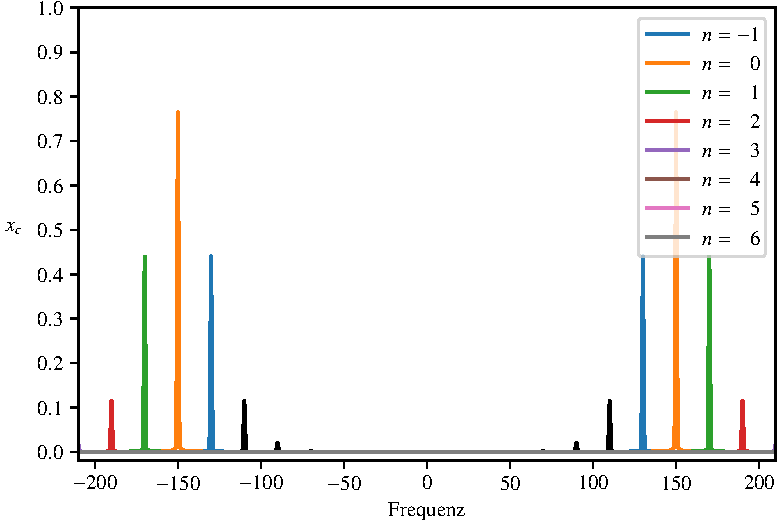
\includegraphics{papers/fm/images/fc150.pdf}
	%%% Creator: Matplotlib, PGF backend
%%
%% To include the figure in your LaTeX document, write
%%   \input{<filename>.pgf}
%%
%% Make sure the required packages are loaded in your preamble
%%   \usepackage{pgf}
%%
%% Also ensure that all the required font packages are loaded; for instance,
%% the lmodern package is sometimes necessary when using math font.
%%   \usepackage{lmodern}
%%
%% Figures using additional raster images can only be included by \input if
%% they are in the same directory as the main LaTeX file. For loading figures
%% from other directories you can use the `import` package
%%   \usepackage{import}
%%
%% and then include the figures with
%%   \import{<path to file>}{<filename>.pgf}
%%
%% Matplotlib used the following preamble
%%
\begingroup%
\makeatletter%
\begin{pgfpicture}%
\pgfpathrectangle{\pgfpointorigin}{\pgfqpoint{6.000000in}{4.000000in}}%
\pgfusepath{use as bounding box, clip}%
\begin{pgfscope}%
\pgfsetbuttcap%
\pgfsetmiterjoin%
\pgfsetlinewidth{0.000000pt}%
\definecolor{currentstroke}{rgb}{1.000000,1.000000,1.000000}%
\pgfsetstrokecolor{currentstroke}%
\pgfsetstrokeopacity{0.000000}%
\pgfsetdash{}{0pt}%
\pgfpathmoveto{\pgfqpoint{0.000000in}{0.000000in}}%
\pgfpathlineto{\pgfqpoint{6.000000in}{0.000000in}}%
\pgfpathlineto{\pgfqpoint{6.000000in}{4.000000in}}%
\pgfpathlineto{\pgfqpoint{0.000000in}{4.000000in}}%
\pgfpathlineto{\pgfqpoint{0.000000in}{0.000000in}}%
\pgfpathclose%
\pgfusepath{}%
\end{pgfscope}%
\begin{pgfscope}%
\pgfsetbuttcap%
\pgfsetmiterjoin%
\definecolor{currentfill}{rgb}{1.000000,1.000000,1.000000}%
\pgfsetfillcolor{currentfill}%
\pgfsetlinewidth{0.000000pt}%
\definecolor{currentstroke}{rgb}{0.000000,0.000000,0.000000}%
\pgfsetstrokecolor{currentstroke}%
\pgfsetstrokeopacity{0.000000}%
\pgfsetdash{}{0pt}%
\pgfpathmoveto{\pgfqpoint{0.750000in}{0.500000in}}%
\pgfpathlineto{\pgfqpoint{5.400000in}{0.500000in}}%
\pgfpathlineto{\pgfqpoint{5.400000in}{3.520000in}}%
\pgfpathlineto{\pgfqpoint{0.750000in}{3.520000in}}%
\pgfpathlineto{\pgfqpoint{0.750000in}{0.500000in}}%
\pgfpathclose%
\pgfusepath{fill}%
\end{pgfscope}%
\begin{pgfscope}%
\pgfsetbuttcap%
\pgfsetroundjoin%
\definecolor{currentfill}{rgb}{0.000000,0.000000,0.000000}%
\pgfsetfillcolor{currentfill}%
\pgfsetlinewidth{0.803000pt}%
\definecolor{currentstroke}{rgb}{0.000000,0.000000,0.000000}%
\pgfsetstrokecolor{currentstroke}%
\pgfsetdash{}{0pt}%
\pgfsys@defobject{currentmarker}{\pgfqpoint{0.000000in}{-0.048611in}}{\pgfqpoint{0.000000in}{0.000000in}}{%
\pgfpathmoveto{\pgfqpoint{0.000000in}{0.000000in}}%
\pgfpathlineto{\pgfqpoint{0.000000in}{-0.048611in}}%
\pgfusepath{stroke,fill}%
}%
\begin{pgfscope}%
\pgfsys@transformshift{0.860714in}{0.500000in}%
\pgfsys@useobject{currentmarker}{}%
\end{pgfscope}%
\end{pgfscope}%
\begin{pgfscope}%
\definecolor{textcolor}{rgb}{0.000000,0.000000,0.000000}%
\pgfsetstrokecolor{textcolor}%
\pgfsetfillcolor{textcolor}%
\pgftext[x=0.860714in,y=0.402778in,,top]{\color{textcolor}\rmfamily\fontsize{10.000000}{12.000000}\selectfont \(\displaystyle {\ensuremath{-}200}\)}%
\end{pgfscope}%
\begin{pgfscope}%
\pgfsetbuttcap%
\pgfsetroundjoin%
\definecolor{currentfill}{rgb}{0.000000,0.000000,0.000000}%
\pgfsetfillcolor{currentfill}%
\pgfsetlinewidth{0.803000pt}%
\definecolor{currentstroke}{rgb}{0.000000,0.000000,0.000000}%
\pgfsetstrokecolor{currentstroke}%
\pgfsetdash{}{0pt}%
\pgfsys@defobject{currentmarker}{\pgfqpoint{0.000000in}{-0.048611in}}{\pgfqpoint{0.000000in}{0.000000in}}{%
\pgfpathmoveto{\pgfqpoint{0.000000in}{0.000000in}}%
\pgfpathlineto{\pgfqpoint{0.000000in}{-0.048611in}}%
\pgfusepath{stroke,fill}%
}%
\begin{pgfscope}%
\pgfsys@transformshift{1.414286in}{0.500000in}%
\pgfsys@useobject{currentmarker}{}%
\end{pgfscope}%
\end{pgfscope}%
\begin{pgfscope}%
\definecolor{textcolor}{rgb}{0.000000,0.000000,0.000000}%
\pgfsetstrokecolor{textcolor}%
\pgfsetfillcolor{textcolor}%
\pgftext[x=1.414286in,y=0.402778in,,top]{\color{textcolor}\rmfamily\fontsize{10.000000}{12.000000}\selectfont \(\displaystyle {\ensuremath{-}150}\)}%
\end{pgfscope}%
\begin{pgfscope}%
\pgfsetbuttcap%
\pgfsetroundjoin%
\definecolor{currentfill}{rgb}{0.000000,0.000000,0.000000}%
\pgfsetfillcolor{currentfill}%
\pgfsetlinewidth{0.803000pt}%
\definecolor{currentstroke}{rgb}{0.000000,0.000000,0.000000}%
\pgfsetstrokecolor{currentstroke}%
\pgfsetdash{}{0pt}%
\pgfsys@defobject{currentmarker}{\pgfqpoint{0.000000in}{-0.048611in}}{\pgfqpoint{0.000000in}{0.000000in}}{%
\pgfpathmoveto{\pgfqpoint{0.000000in}{0.000000in}}%
\pgfpathlineto{\pgfqpoint{0.000000in}{-0.048611in}}%
\pgfusepath{stroke,fill}%
}%
\begin{pgfscope}%
\pgfsys@transformshift{1.967857in}{0.500000in}%
\pgfsys@useobject{currentmarker}{}%
\end{pgfscope}%
\end{pgfscope}%
\begin{pgfscope}%
\definecolor{textcolor}{rgb}{0.000000,0.000000,0.000000}%
\pgfsetstrokecolor{textcolor}%
\pgfsetfillcolor{textcolor}%
\pgftext[x=1.967857in,y=0.402778in,,top]{\color{textcolor}\rmfamily\fontsize{10.000000}{12.000000}\selectfont \(\displaystyle {\ensuremath{-}100}\)}%
\end{pgfscope}%
\begin{pgfscope}%
\pgfsetbuttcap%
\pgfsetroundjoin%
\definecolor{currentfill}{rgb}{0.000000,0.000000,0.000000}%
\pgfsetfillcolor{currentfill}%
\pgfsetlinewidth{0.803000pt}%
\definecolor{currentstroke}{rgb}{0.000000,0.000000,0.000000}%
\pgfsetstrokecolor{currentstroke}%
\pgfsetdash{}{0pt}%
\pgfsys@defobject{currentmarker}{\pgfqpoint{0.000000in}{-0.048611in}}{\pgfqpoint{0.000000in}{0.000000in}}{%
\pgfpathmoveto{\pgfqpoint{0.000000in}{0.000000in}}%
\pgfpathlineto{\pgfqpoint{0.000000in}{-0.048611in}}%
\pgfusepath{stroke,fill}%
}%
\begin{pgfscope}%
\pgfsys@transformshift{2.521429in}{0.500000in}%
\pgfsys@useobject{currentmarker}{}%
\end{pgfscope}%
\end{pgfscope}%
\begin{pgfscope}%
\definecolor{textcolor}{rgb}{0.000000,0.000000,0.000000}%
\pgfsetstrokecolor{textcolor}%
\pgfsetfillcolor{textcolor}%
\pgftext[x=2.521429in,y=0.402778in,,top]{\color{textcolor}\rmfamily\fontsize{10.000000}{12.000000}\selectfont \(\displaystyle {\ensuremath{-}50}\)}%
\end{pgfscope}%
\begin{pgfscope}%
\pgfsetbuttcap%
\pgfsetroundjoin%
\definecolor{currentfill}{rgb}{0.000000,0.000000,0.000000}%
\pgfsetfillcolor{currentfill}%
\pgfsetlinewidth{0.803000pt}%
\definecolor{currentstroke}{rgb}{0.000000,0.000000,0.000000}%
\pgfsetstrokecolor{currentstroke}%
\pgfsetdash{}{0pt}%
\pgfsys@defobject{currentmarker}{\pgfqpoint{0.000000in}{-0.048611in}}{\pgfqpoint{0.000000in}{0.000000in}}{%
\pgfpathmoveto{\pgfqpoint{0.000000in}{0.000000in}}%
\pgfpathlineto{\pgfqpoint{0.000000in}{-0.048611in}}%
\pgfusepath{stroke,fill}%
}%
\begin{pgfscope}%
\pgfsys@transformshift{3.075000in}{0.500000in}%
\pgfsys@useobject{currentmarker}{}%
\end{pgfscope}%
\end{pgfscope}%
\begin{pgfscope}%
\definecolor{textcolor}{rgb}{0.000000,0.000000,0.000000}%
\pgfsetstrokecolor{textcolor}%
\pgfsetfillcolor{textcolor}%
\pgftext[x=3.075000in,y=0.402778in,,top]{\color{textcolor}\rmfamily\fontsize{10.000000}{12.000000}\selectfont \(\displaystyle {0}\)}%
\end{pgfscope}%
\begin{pgfscope}%
\pgfsetbuttcap%
\pgfsetroundjoin%
\definecolor{currentfill}{rgb}{0.000000,0.000000,0.000000}%
\pgfsetfillcolor{currentfill}%
\pgfsetlinewidth{0.803000pt}%
\definecolor{currentstroke}{rgb}{0.000000,0.000000,0.000000}%
\pgfsetstrokecolor{currentstroke}%
\pgfsetdash{}{0pt}%
\pgfsys@defobject{currentmarker}{\pgfqpoint{0.000000in}{-0.048611in}}{\pgfqpoint{0.000000in}{0.000000in}}{%
\pgfpathmoveto{\pgfqpoint{0.000000in}{0.000000in}}%
\pgfpathlineto{\pgfqpoint{0.000000in}{-0.048611in}}%
\pgfusepath{stroke,fill}%
}%
\begin{pgfscope}%
\pgfsys@transformshift{3.628571in}{0.500000in}%
\pgfsys@useobject{currentmarker}{}%
\end{pgfscope}%
\end{pgfscope}%
\begin{pgfscope}%
\definecolor{textcolor}{rgb}{0.000000,0.000000,0.000000}%
\pgfsetstrokecolor{textcolor}%
\pgfsetfillcolor{textcolor}%
\pgftext[x=3.628571in,y=0.402778in,,top]{\color{textcolor}\rmfamily\fontsize{10.000000}{12.000000}\selectfont \(\displaystyle {50}\)}%
\end{pgfscope}%
\begin{pgfscope}%
\pgfsetbuttcap%
\pgfsetroundjoin%
\definecolor{currentfill}{rgb}{0.000000,0.000000,0.000000}%
\pgfsetfillcolor{currentfill}%
\pgfsetlinewidth{0.803000pt}%
\definecolor{currentstroke}{rgb}{0.000000,0.000000,0.000000}%
\pgfsetstrokecolor{currentstroke}%
\pgfsetdash{}{0pt}%
\pgfsys@defobject{currentmarker}{\pgfqpoint{0.000000in}{-0.048611in}}{\pgfqpoint{0.000000in}{0.000000in}}{%
\pgfpathmoveto{\pgfqpoint{0.000000in}{0.000000in}}%
\pgfpathlineto{\pgfqpoint{0.000000in}{-0.048611in}}%
\pgfusepath{stroke,fill}%
}%
\begin{pgfscope}%
\pgfsys@transformshift{4.182143in}{0.500000in}%
\pgfsys@useobject{currentmarker}{}%
\end{pgfscope}%
\end{pgfscope}%
\begin{pgfscope}%
\definecolor{textcolor}{rgb}{0.000000,0.000000,0.000000}%
\pgfsetstrokecolor{textcolor}%
\pgfsetfillcolor{textcolor}%
\pgftext[x=4.182143in,y=0.402778in,,top]{\color{textcolor}\rmfamily\fontsize{10.000000}{12.000000}\selectfont \(\displaystyle {100}\)}%
\end{pgfscope}%
\begin{pgfscope}%
\pgfsetbuttcap%
\pgfsetroundjoin%
\definecolor{currentfill}{rgb}{0.000000,0.000000,0.000000}%
\pgfsetfillcolor{currentfill}%
\pgfsetlinewidth{0.803000pt}%
\definecolor{currentstroke}{rgb}{0.000000,0.000000,0.000000}%
\pgfsetstrokecolor{currentstroke}%
\pgfsetdash{}{0pt}%
\pgfsys@defobject{currentmarker}{\pgfqpoint{0.000000in}{-0.048611in}}{\pgfqpoint{0.000000in}{0.000000in}}{%
\pgfpathmoveto{\pgfqpoint{0.000000in}{0.000000in}}%
\pgfpathlineto{\pgfqpoint{0.000000in}{-0.048611in}}%
\pgfusepath{stroke,fill}%
}%
\begin{pgfscope}%
\pgfsys@transformshift{4.735714in}{0.500000in}%
\pgfsys@useobject{currentmarker}{}%
\end{pgfscope}%
\end{pgfscope}%
\begin{pgfscope}%
\definecolor{textcolor}{rgb}{0.000000,0.000000,0.000000}%
\pgfsetstrokecolor{textcolor}%
\pgfsetfillcolor{textcolor}%
\pgftext[x=4.735714in,y=0.402778in,,top]{\color{textcolor}\rmfamily\fontsize{10.000000}{12.000000}\selectfont \(\displaystyle {150}\)}%
\end{pgfscope}%
\begin{pgfscope}%
\pgfsetbuttcap%
\pgfsetroundjoin%
\definecolor{currentfill}{rgb}{0.000000,0.000000,0.000000}%
\pgfsetfillcolor{currentfill}%
\pgfsetlinewidth{0.803000pt}%
\definecolor{currentstroke}{rgb}{0.000000,0.000000,0.000000}%
\pgfsetstrokecolor{currentstroke}%
\pgfsetdash{}{0pt}%
\pgfsys@defobject{currentmarker}{\pgfqpoint{0.000000in}{-0.048611in}}{\pgfqpoint{0.000000in}{0.000000in}}{%
\pgfpathmoveto{\pgfqpoint{0.000000in}{0.000000in}}%
\pgfpathlineto{\pgfqpoint{0.000000in}{-0.048611in}}%
\pgfusepath{stroke,fill}%
}%
\begin{pgfscope}%
\pgfsys@transformshift{5.289286in}{0.500000in}%
\pgfsys@useobject{currentmarker}{}%
\end{pgfscope}%
\end{pgfscope}%
\begin{pgfscope}%
\definecolor{textcolor}{rgb}{0.000000,0.000000,0.000000}%
\pgfsetstrokecolor{textcolor}%
\pgfsetfillcolor{textcolor}%
\pgftext[x=5.289286in,y=0.402778in,,top]{\color{textcolor}\rmfamily\fontsize{10.000000}{12.000000}\selectfont \(\displaystyle {200}\)}%
\end{pgfscope}%
\begin{pgfscope}%
\definecolor{textcolor}{rgb}{0.000000,0.000000,0.000000}%
\pgfsetstrokecolor{textcolor}%
\pgfsetfillcolor{textcolor}%
\pgftext[x=3.075000in,y=0.223766in,,top]{\color{textcolor}\rmfamily\fontsize{10.000000}{12.000000}\selectfont Frequenz}%
\end{pgfscope}%
\begin{pgfscope}%
\pgfsetbuttcap%
\pgfsetroundjoin%
\definecolor{currentfill}{rgb}{0.000000,0.000000,0.000000}%
\pgfsetfillcolor{currentfill}%
\pgfsetlinewidth{0.803000pt}%
\definecolor{currentstroke}{rgb}{0.000000,0.000000,0.000000}%
\pgfsetstrokecolor{currentstroke}%
\pgfsetdash{}{0pt}%
\pgfsys@defobject{currentmarker}{\pgfqpoint{-0.048611in}{0.000000in}}{\pgfqpoint{-0.000000in}{0.000000in}}{%
\pgfpathmoveto{\pgfqpoint{-0.000000in}{0.000000in}}%
\pgfpathlineto{\pgfqpoint{-0.048611in}{0.000000in}}%
\pgfusepath{stroke,fill}%
}%
\begin{pgfscope}%
\pgfsys@transformshift{0.750000in}{0.559216in}%
\pgfsys@useobject{currentmarker}{}%
\end{pgfscope}%
\end{pgfscope}%
\begin{pgfscope}%
\definecolor{textcolor}{rgb}{0.000000,0.000000,0.000000}%
\pgfsetstrokecolor{textcolor}%
\pgfsetfillcolor{textcolor}%
\pgftext[x=0.475308in, y=0.510990in, left, base]{\color{textcolor}\rmfamily\fontsize{10.000000}{12.000000}\selectfont \(\displaystyle {0.0}\)}%
\end{pgfscope}%
\begin{pgfscope}%
\pgfsetbuttcap%
\pgfsetroundjoin%
\definecolor{currentfill}{rgb}{0.000000,0.000000,0.000000}%
\pgfsetfillcolor{currentfill}%
\pgfsetlinewidth{0.803000pt}%
\definecolor{currentstroke}{rgb}{0.000000,0.000000,0.000000}%
\pgfsetstrokecolor{currentstroke}%
\pgfsetdash{}{0pt}%
\pgfsys@defobject{currentmarker}{\pgfqpoint{-0.048611in}{0.000000in}}{\pgfqpoint{-0.000000in}{0.000000in}}{%
\pgfpathmoveto{\pgfqpoint{-0.000000in}{0.000000in}}%
\pgfpathlineto{\pgfqpoint{-0.048611in}{0.000000in}}%
\pgfusepath{stroke,fill}%
}%
\begin{pgfscope}%
\pgfsys@transformshift{0.750000in}{0.855294in}%
\pgfsys@useobject{currentmarker}{}%
\end{pgfscope}%
\end{pgfscope}%
\begin{pgfscope}%
\definecolor{textcolor}{rgb}{0.000000,0.000000,0.000000}%
\pgfsetstrokecolor{textcolor}%
\pgfsetfillcolor{textcolor}%
\pgftext[x=0.475308in, y=0.807069in, left, base]{\color{textcolor}\rmfamily\fontsize{10.000000}{12.000000}\selectfont \(\displaystyle {0.1}\)}%
\end{pgfscope}%
\begin{pgfscope}%
\pgfsetbuttcap%
\pgfsetroundjoin%
\definecolor{currentfill}{rgb}{0.000000,0.000000,0.000000}%
\pgfsetfillcolor{currentfill}%
\pgfsetlinewidth{0.803000pt}%
\definecolor{currentstroke}{rgb}{0.000000,0.000000,0.000000}%
\pgfsetstrokecolor{currentstroke}%
\pgfsetdash{}{0pt}%
\pgfsys@defobject{currentmarker}{\pgfqpoint{-0.048611in}{0.000000in}}{\pgfqpoint{-0.000000in}{0.000000in}}{%
\pgfpathmoveto{\pgfqpoint{-0.000000in}{0.000000in}}%
\pgfpathlineto{\pgfqpoint{-0.048611in}{0.000000in}}%
\pgfusepath{stroke,fill}%
}%
\begin{pgfscope}%
\pgfsys@transformshift{0.750000in}{1.151373in}%
\pgfsys@useobject{currentmarker}{}%
\end{pgfscope}%
\end{pgfscope}%
\begin{pgfscope}%
\definecolor{textcolor}{rgb}{0.000000,0.000000,0.000000}%
\pgfsetstrokecolor{textcolor}%
\pgfsetfillcolor{textcolor}%
\pgftext[x=0.475308in, y=1.103147in, left, base]{\color{textcolor}\rmfamily\fontsize{10.000000}{12.000000}\selectfont \(\displaystyle {0.2}\)}%
\end{pgfscope}%
\begin{pgfscope}%
\pgfsetbuttcap%
\pgfsetroundjoin%
\definecolor{currentfill}{rgb}{0.000000,0.000000,0.000000}%
\pgfsetfillcolor{currentfill}%
\pgfsetlinewidth{0.803000pt}%
\definecolor{currentstroke}{rgb}{0.000000,0.000000,0.000000}%
\pgfsetstrokecolor{currentstroke}%
\pgfsetdash{}{0pt}%
\pgfsys@defobject{currentmarker}{\pgfqpoint{-0.048611in}{0.000000in}}{\pgfqpoint{-0.000000in}{0.000000in}}{%
\pgfpathmoveto{\pgfqpoint{-0.000000in}{0.000000in}}%
\pgfpathlineto{\pgfqpoint{-0.048611in}{0.000000in}}%
\pgfusepath{stroke,fill}%
}%
\begin{pgfscope}%
\pgfsys@transformshift{0.750000in}{1.447451in}%
\pgfsys@useobject{currentmarker}{}%
\end{pgfscope}%
\end{pgfscope}%
\begin{pgfscope}%
\definecolor{textcolor}{rgb}{0.000000,0.000000,0.000000}%
\pgfsetstrokecolor{textcolor}%
\pgfsetfillcolor{textcolor}%
\pgftext[x=0.475308in, y=1.399226in, left, base]{\color{textcolor}\rmfamily\fontsize{10.000000}{12.000000}\selectfont \(\displaystyle {0.3}\)}%
\end{pgfscope}%
\begin{pgfscope}%
\pgfsetbuttcap%
\pgfsetroundjoin%
\definecolor{currentfill}{rgb}{0.000000,0.000000,0.000000}%
\pgfsetfillcolor{currentfill}%
\pgfsetlinewidth{0.803000pt}%
\definecolor{currentstroke}{rgb}{0.000000,0.000000,0.000000}%
\pgfsetstrokecolor{currentstroke}%
\pgfsetdash{}{0pt}%
\pgfsys@defobject{currentmarker}{\pgfqpoint{-0.048611in}{0.000000in}}{\pgfqpoint{-0.000000in}{0.000000in}}{%
\pgfpathmoveto{\pgfqpoint{-0.000000in}{0.000000in}}%
\pgfpathlineto{\pgfqpoint{-0.048611in}{0.000000in}}%
\pgfusepath{stroke,fill}%
}%
\begin{pgfscope}%
\pgfsys@transformshift{0.750000in}{1.743529in}%
\pgfsys@useobject{currentmarker}{}%
\end{pgfscope}%
\end{pgfscope}%
\begin{pgfscope}%
\definecolor{textcolor}{rgb}{0.000000,0.000000,0.000000}%
\pgfsetstrokecolor{textcolor}%
\pgfsetfillcolor{textcolor}%
\pgftext[x=0.475308in, y=1.695304in, left, base]{\color{textcolor}\rmfamily\fontsize{10.000000}{12.000000}\selectfont \(\displaystyle {0.4}\)}%
\end{pgfscope}%
\begin{pgfscope}%
\pgfsetbuttcap%
\pgfsetroundjoin%
\definecolor{currentfill}{rgb}{0.000000,0.000000,0.000000}%
\pgfsetfillcolor{currentfill}%
\pgfsetlinewidth{0.803000pt}%
\definecolor{currentstroke}{rgb}{0.000000,0.000000,0.000000}%
\pgfsetstrokecolor{currentstroke}%
\pgfsetdash{}{0pt}%
\pgfsys@defobject{currentmarker}{\pgfqpoint{-0.048611in}{0.000000in}}{\pgfqpoint{-0.000000in}{0.000000in}}{%
\pgfpathmoveto{\pgfqpoint{-0.000000in}{0.000000in}}%
\pgfpathlineto{\pgfqpoint{-0.048611in}{0.000000in}}%
\pgfusepath{stroke,fill}%
}%
\begin{pgfscope}%
\pgfsys@transformshift{0.750000in}{2.039608in}%
\pgfsys@useobject{currentmarker}{}%
\end{pgfscope}%
\end{pgfscope}%
\begin{pgfscope}%
\definecolor{textcolor}{rgb}{0.000000,0.000000,0.000000}%
\pgfsetstrokecolor{textcolor}%
\pgfsetfillcolor{textcolor}%
\pgftext[x=0.475308in, y=1.991383in, left, base]{\color{textcolor}\rmfamily\fontsize{10.000000}{12.000000}\selectfont \(\displaystyle {0.5}\)}%
\end{pgfscope}%
\begin{pgfscope}%
\pgfsetbuttcap%
\pgfsetroundjoin%
\definecolor{currentfill}{rgb}{0.000000,0.000000,0.000000}%
\pgfsetfillcolor{currentfill}%
\pgfsetlinewidth{0.803000pt}%
\definecolor{currentstroke}{rgb}{0.000000,0.000000,0.000000}%
\pgfsetstrokecolor{currentstroke}%
\pgfsetdash{}{0pt}%
\pgfsys@defobject{currentmarker}{\pgfqpoint{-0.048611in}{0.000000in}}{\pgfqpoint{-0.000000in}{0.000000in}}{%
\pgfpathmoveto{\pgfqpoint{-0.000000in}{0.000000in}}%
\pgfpathlineto{\pgfqpoint{-0.048611in}{0.000000in}}%
\pgfusepath{stroke,fill}%
}%
\begin{pgfscope}%
\pgfsys@transformshift{0.750000in}{2.335686in}%
\pgfsys@useobject{currentmarker}{}%
\end{pgfscope}%
\end{pgfscope}%
\begin{pgfscope}%
\definecolor{textcolor}{rgb}{0.000000,0.000000,0.000000}%
\pgfsetstrokecolor{textcolor}%
\pgfsetfillcolor{textcolor}%
\pgftext[x=0.475308in, y=2.287461in, left, base]{\color{textcolor}\rmfamily\fontsize{10.000000}{12.000000}\selectfont \(\displaystyle {0.6}\)}%
\end{pgfscope}%
\begin{pgfscope}%
\pgfsetbuttcap%
\pgfsetroundjoin%
\definecolor{currentfill}{rgb}{0.000000,0.000000,0.000000}%
\pgfsetfillcolor{currentfill}%
\pgfsetlinewidth{0.803000pt}%
\definecolor{currentstroke}{rgb}{0.000000,0.000000,0.000000}%
\pgfsetstrokecolor{currentstroke}%
\pgfsetdash{}{0pt}%
\pgfsys@defobject{currentmarker}{\pgfqpoint{-0.048611in}{0.000000in}}{\pgfqpoint{-0.000000in}{0.000000in}}{%
\pgfpathmoveto{\pgfqpoint{-0.000000in}{0.000000in}}%
\pgfpathlineto{\pgfqpoint{-0.048611in}{0.000000in}}%
\pgfusepath{stroke,fill}%
}%
\begin{pgfscope}%
\pgfsys@transformshift{0.750000in}{2.631765in}%
\pgfsys@useobject{currentmarker}{}%
\end{pgfscope}%
\end{pgfscope}%
\begin{pgfscope}%
\definecolor{textcolor}{rgb}{0.000000,0.000000,0.000000}%
\pgfsetstrokecolor{textcolor}%
\pgfsetfillcolor{textcolor}%
\pgftext[x=0.475308in, y=2.583539in, left, base]{\color{textcolor}\rmfamily\fontsize{10.000000}{12.000000}\selectfont \(\displaystyle {0.7}\)}%
\end{pgfscope}%
\begin{pgfscope}%
\pgfsetbuttcap%
\pgfsetroundjoin%
\definecolor{currentfill}{rgb}{0.000000,0.000000,0.000000}%
\pgfsetfillcolor{currentfill}%
\pgfsetlinewidth{0.803000pt}%
\definecolor{currentstroke}{rgb}{0.000000,0.000000,0.000000}%
\pgfsetstrokecolor{currentstroke}%
\pgfsetdash{}{0pt}%
\pgfsys@defobject{currentmarker}{\pgfqpoint{-0.048611in}{0.000000in}}{\pgfqpoint{-0.000000in}{0.000000in}}{%
\pgfpathmoveto{\pgfqpoint{-0.000000in}{0.000000in}}%
\pgfpathlineto{\pgfqpoint{-0.048611in}{0.000000in}}%
\pgfusepath{stroke,fill}%
}%
\begin{pgfscope}%
\pgfsys@transformshift{0.750000in}{2.927843in}%
\pgfsys@useobject{currentmarker}{}%
\end{pgfscope}%
\end{pgfscope}%
\begin{pgfscope}%
\definecolor{textcolor}{rgb}{0.000000,0.000000,0.000000}%
\pgfsetstrokecolor{textcolor}%
\pgfsetfillcolor{textcolor}%
\pgftext[x=0.475308in, y=2.879618in, left, base]{\color{textcolor}\rmfamily\fontsize{10.000000}{12.000000}\selectfont \(\displaystyle {0.8}\)}%
\end{pgfscope}%
\begin{pgfscope}%
\pgfsetbuttcap%
\pgfsetroundjoin%
\definecolor{currentfill}{rgb}{0.000000,0.000000,0.000000}%
\pgfsetfillcolor{currentfill}%
\pgfsetlinewidth{0.803000pt}%
\definecolor{currentstroke}{rgb}{0.000000,0.000000,0.000000}%
\pgfsetstrokecolor{currentstroke}%
\pgfsetdash{}{0pt}%
\pgfsys@defobject{currentmarker}{\pgfqpoint{-0.048611in}{0.000000in}}{\pgfqpoint{-0.000000in}{0.000000in}}{%
\pgfpathmoveto{\pgfqpoint{-0.000000in}{0.000000in}}%
\pgfpathlineto{\pgfqpoint{-0.048611in}{0.000000in}}%
\pgfusepath{stroke,fill}%
}%
\begin{pgfscope}%
\pgfsys@transformshift{0.750000in}{3.223922in}%
\pgfsys@useobject{currentmarker}{}%
\end{pgfscope}%
\end{pgfscope}%
\begin{pgfscope}%
\definecolor{textcolor}{rgb}{0.000000,0.000000,0.000000}%
\pgfsetstrokecolor{textcolor}%
\pgfsetfillcolor{textcolor}%
\pgftext[x=0.475308in, y=3.175696in, left, base]{\color{textcolor}\rmfamily\fontsize{10.000000}{12.000000}\selectfont \(\displaystyle {0.9}\)}%
\end{pgfscope}%
\begin{pgfscope}%
\pgfsetbuttcap%
\pgfsetroundjoin%
\definecolor{currentfill}{rgb}{0.000000,0.000000,0.000000}%
\pgfsetfillcolor{currentfill}%
\pgfsetlinewidth{0.803000pt}%
\definecolor{currentstroke}{rgb}{0.000000,0.000000,0.000000}%
\pgfsetstrokecolor{currentstroke}%
\pgfsetdash{}{0pt}%
\pgfsys@defobject{currentmarker}{\pgfqpoint{-0.048611in}{0.000000in}}{\pgfqpoint{-0.000000in}{0.000000in}}{%
\pgfpathmoveto{\pgfqpoint{-0.000000in}{0.000000in}}%
\pgfpathlineto{\pgfqpoint{-0.048611in}{0.000000in}}%
\pgfusepath{stroke,fill}%
}%
\begin{pgfscope}%
\pgfsys@transformshift{0.750000in}{3.520000in}%
\pgfsys@useobject{currentmarker}{}%
\end{pgfscope}%
\end{pgfscope}%
\begin{pgfscope}%
\definecolor{textcolor}{rgb}{0.000000,0.000000,0.000000}%
\pgfsetstrokecolor{textcolor}%
\pgfsetfillcolor{textcolor}%
\pgftext[x=0.475308in, y=3.471775in, left, base]{\color{textcolor}\rmfamily\fontsize{10.000000}{12.000000}\selectfont \(\displaystyle {1.0}\)}%
\end{pgfscope}%
\begin{pgfscope}%
\definecolor{textcolor}{rgb}{0.000000,0.000000,0.000000}%
\pgfsetstrokecolor{textcolor}%
\pgfsetfillcolor{textcolor}%
\pgftext[x=0.319753in,y=2.010000in,,bottom,rotate=00.000000]{\color{textcolor}\rmfamily\fontsize{10.000000}{12.000000}\selectfont \(\displaystyle x_c\)}%
\end{pgfscope}%
\begin{pgfscope}%
\pgfpathrectangle{\pgfqpoint{0.750000in}{0.500000in}}{\pgfqpoint{4.650000in}{3.020000in}}%
\pgfusepath{clip}%
\pgfsetrectcap%
\pgfsetroundjoin%
\pgfsetlinewidth{1.505625pt}%
\definecolor{currentstroke}{rgb}{0.000000,0.000000,0.000000}%
\pgfsetstrokecolor{currentstroke}%
\pgfsetdash{}{0pt}%
\pgfpathmoveto{\pgfqpoint{3.075000in}{0.559216in}}%
\pgfpathlineto{\pgfqpoint{5.413889in}{0.559216in}}%
\pgfpathmoveto{\pgfqpoint{5.413889in}{0.559216in}}%
\pgfpathlineto{\pgfqpoint{0.736111in}{0.559216in}}%
\pgfpathmoveto{\pgfqpoint{0.736111in}{0.559216in}}%
\pgfpathlineto{\pgfqpoint{3.063929in}{0.559216in}}%
\pgfpathlineto{\pgfqpoint{3.063929in}{0.559216in}}%
\pgfusepath{stroke}%
\end{pgfscope}%
\begin{pgfscope}%
\pgfpathrectangle{\pgfqpoint{0.750000in}{0.500000in}}{\pgfqpoint{4.650000in}{3.020000in}}%
\pgfusepath{clip}%
\pgfsetrectcap%
\pgfsetroundjoin%
\pgfsetlinewidth{1.505625pt}%
\definecolor{currentstroke}{rgb}{0.000000,0.000000,0.000000}%
\pgfsetstrokecolor{currentstroke}%
\pgfsetdash{}{0pt}%
\pgfpathmoveto{\pgfqpoint{3.075000in}{0.559216in}}%
\pgfpathlineto{\pgfqpoint{5.413889in}{0.559216in}}%
\pgfpathmoveto{\pgfqpoint{5.413889in}{0.559216in}}%
\pgfpathlineto{\pgfqpoint{0.736111in}{0.559216in}}%
\pgfpathmoveto{\pgfqpoint{0.736111in}{0.559216in}}%
\pgfpathlineto{\pgfqpoint{3.063929in}{0.559216in}}%
\pgfpathlineto{\pgfqpoint{3.063929in}{0.559216in}}%
\pgfusepath{stroke}%
\end{pgfscope}%
\begin{pgfscope}%
\pgfpathrectangle{\pgfqpoint{0.750000in}{0.500000in}}{\pgfqpoint{4.650000in}{3.020000in}}%
\pgfusepath{clip}%
\pgfsetrectcap%
\pgfsetroundjoin%
\pgfsetlinewidth{1.505625pt}%
\definecolor{currentstroke}{rgb}{0.000000,0.000000,0.000000}%
\pgfsetstrokecolor{currentstroke}%
\pgfsetdash{}{0pt}%
\pgfpathmoveto{\pgfqpoint{3.075000in}{0.559217in}}%
\pgfpathlineto{\pgfqpoint{3.838929in}{0.559267in}}%
\pgfpathlineto{\pgfqpoint{3.850000in}{0.566548in}}%
\pgfpathlineto{\pgfqpoint{3.861071in}{0.559267in}}%
\pgfpathlineto{\pgfqpoint{4.536429in}{0.559216in}}%
\pgfpathlineto{\pgfqpoint{5.413889in}{0.559216in}}%
\pgfpathmoveto{\pgfqpoint{5.413889in}{0.559216in}}%
\pgfpathlineto{\pgfqpoint{0.736111in}{0.559216in}}%
\pgfpathmoveto{\pgfqpoint{0.736111in}{0.559216in}}%
\pgfpathlineto{\pgfqpoint{2.288929in}{0.559267in}}%
\pgfpathlineto{\pgfqpoint{2.300000in}{0.566548in}}%
\pgfpathlineto{\pgfqpoint{2.311071in}{0.559267in}}%
\pgfpathlineto{\pgfqpoint{2.997500in}{0.559217in}}%
\pgfpathlineto{\pgfqpoint{3.063929in}{0.559217in}}%
\pgfpathlineto{\pgfqpoint{3.063929in}{0.559217in}}%
\pgfusepath{stroke}%
\end{pgfscope}%
\begin{pgfscope}%
\pgfpathrectangle{\pgfqpoint{0.750000in}{0.500000in}}{\pgfqpoint{4.650000in}{3.020000in}}%
\pgfusepath{clip}%
\pgfsetrectcap%
\pgfsetroundjoin%
\pgfsetlinewidth{1.505625pt}%
\definecolor{currentstroke}{rgb}{0.000000,0.000000,0.000000}%
\pgfsetstrokecolor{currentstroke}%
\pgfsetdash{}{0pt}%
\pgfpathmoveto{\pgfqpoint{3.075000in}{0.559222in}}%
\pgfpathlineto{\pgfqpoint{4.060357in}{0.559731in}}%
\pgfpathlineto{\pgfqpoint{4.071429in}{0.617130in}}%
\pgfpathlineto{\pgfqpoint{4.082500in}{0.559743in}}%
\pgfpathlineto{\pgfqpoint{4.160000in}{0.559282in}}%
\pgfpathlineto{\pgfqpoint{5.413889in}{0.559221in}}%
\pgfpathmoveto{\pgfqpoint{5.413889in}{0.559216in}}%
\pgfpathlineto{\pgfqpoint{0.736111in}{0.559216in}}%
\pgfpathmoveto{\pgfqpoint{0.736111in}{0.559221in}}%
\pgfpathlineto{\pgfqpoint{2.067500in}{0.559743in}}%
\pgfpathlineto{\pgfqpoint{2.078571in}{0.617130in}}%
\pgfpathlineto{\pgfqpoint{2.089643in}{0.559731in}}%
\pgfpathlineto{\pgfqpoint{2.167143in}{0.559280in}}%
\pgfpathlineto{\pgfqpoint{3.063929in}{0.559222in}}%
\pgfpathlineto{\pgfqpoint{3.063929in}{0.559222in}}%
\pgfusepath{stroke}%
\end{pgfscope}%
\begin{pgfscope}%
\pgfpathrectangle{\pgfqpoint{0.750000in}{0.500000in}}{\pgfqpoint{4.650000in}{3.020000in}}%
\pgfusepath{clip}%
\pgfsetrectcap%
\pgfsetroundjoin%
\pgfsetlinewidth{1.505625pt}%
\definecolor{currentstroke}{rgb}{0.000000,0.000000,0.000000}%
\pgfsetstrokecolor{currentstroke}%
\pgfsetdash{}{0pt}%
\pgfpathmoveto{\pgfqpoint{3.075000in}{0.559256in}}%
\pgfpathlineto{\pgfqpoint{4.259643in}{0.560453in}}%
\pgfpathlineto{\pgfqpoint{4.281786in}{0.562912in}}%
\pgfpathlineto{\pgfqpoint{4.292857in}{0.899347in}}%
\pgfpathlineto{\pgfqpoint{4.303929in}{0.563004in}}%
\pgfpathlineto{\pgfqpoint{4.326071in}{0.560473in}}%
\pgfpathlineto{\pgfqpoint{4.403571in}{0.559596in}}%
\pgfpathlineto{\pgfqpoint{5.001429in}{0.559279in}}%
\pgfpathlineto{\pgfqpoint{5.413889in}{0.559258in}}%
\pgfpathmoveto{\pgfqpoint{5.413889in}{0.559218in}}%
\pgfpathlineto{\pgfqpoint{0.736111in}{0.559218in}}%
\pgfpathmoveto{\pgfqpoint{0.736111in}{0.559258in}}%
\pgfpathlineto{\pgfqpoint{1.823929in}{0.560473in}}%
\pgfpathlineto{\pgfqpoint{1.846071in}{0.563004in}}%
\pgfpathlineto{\pgfqpoint{1.857143in}{0.899347in}}%
\pgfpathlineto{\pgfqpoint{1.868214in}{0.562912in}}%
\pgfpathlineto{\pgfqpoint{1.890357in}{0.560453in}}%
\pgfpathlineto{\pgfqpoint{1.967857in}{0.559584in}}%
\pgfpathlineto{\pgfqpoint{2.565714in}{0.559272in}}%
\pgfpathlineto{\pgfqpoint{3.063929in}{0.559256in}}%
\pgfpathlineto{\pgfqpoint{3.063929in}{0.559256in}}%
\pgfusepath{stroke}%
\end{pgfscope}%
\begin{pgfscope}%
\pgfpathrectangle{\pgfqpoint{0.750000in}{0.500000in}}{\pgfqpoint{4.650000in}{3.020000in}}%
\pgfusepath{clip}%
\pgfsetrectcap%
\pgfsetroundjoin%
\pgfsetlinewidth{1.505625pt}%
\definecolor{currentstroke}{rgb}{0.121569,0.466667,0.705882}%
\pgfsetstrokecolor{currentstroke}%
\pgfsetdash{}{0pt}%
\pgfpathmoveto{\pgfqpoint{3.075000in}{0.559464in}}%
\pgfpathlineto{\pgfqpoint{4.403571in}{0.560962in}}%
\pgfpathlineto{\pgfqpoint{4.470000in}{0.563489in}}%
\pgfpathlineto{\pgfqpoint{4.492143in}{0.567682in}}%
\pgfpathlineto{\pgfqpoint{4.503214in}{0.575986in}}%
\pgfpathlineto{\pgfqpoint{4.514286in}{1.861801in}}%
\pgfpathlineto{\pgfqpoint{4.525357in}{0.576321in}}%
\pgfpathlineto{\pgfqpoint{4.536429in}{0.567686in}}%
\pgfpathlineto{\pgfqpoint{4.558571in}{0.563411in}}%
\pgfpathlineto{\pgfqpoint{4.602857in}{0.561285in}}%
\pgfpathlineto{\pgfqpoint{4.724643in}{0.560059in}}%
\pgfpathlineto{\pgfqpoint{5.267143in}{0.559425in}}%
\pgfpathlineto{\pgfqpoint{5.413889in}{0.559386in}}%
\pgfpathmoveto{\pgfqpoint{5.413889in}{0.559219in}}%
\pgfpathlineto{\pgfqpoint{0.736111in}{0.559219in}}%
\pgfpathmoveto{\pgfqpoint{0.736111in}{0.559386in}}%
\pgfpathlineto{\pgfqpoint{1.536071in}{0.561049in}}%
\pgfpathlineto{\pgfqpoint{1.591429in}{0.563411in}}%
\pgfpathlineto{\pgfqpoint{1.613571in}{0.567686in}}%
\pgfpathlineto{\pgfqpoint{1.624643in}{0.576321in}}%
\pgfpathlineto{\pgfqpoint{1.635714in}{1.861801in}}%
\pgfpathlineto{\pgfqpoint{1.646786in}{0.575986in}}%
\pgfpathlineto{\pgfqpoint{1.657857in}{0.567682in}}%
\pgfpathlineto{\pgfqpoint{1.680000in}{0.563489in}}%
\pgfpathlineto{\pgfqpoint{1.724286in}{0.561384in}}%
\pgfpathlineto{\pgfqpoint{1.846071in}{0.560164in}}%
\pgfpathlineto{\pgfqpoint{2.388571in}{0.559540in}}%
\pgfpathlineto{\pgfqpoint{3.063929in}{0.559464in}}%
\pgfpathlineto{\pgfqpoint{3.063929in}{0.559464in}}%
\pgfusepath{stroke}%
\end{pgfscope}%
\begin{pgfscope}%
\pgfpathrectangle{\pgfqpoint{0.750000in}{0.500000in}}{\pgfqpoint{4.650000in}{3.020000in}}%
\pgfusepath{clip}%
\pgfsetrectcap%
\pgfsetroundjoin%
\pgfsetlinewidth{1.505625pt}%
\definecolor{currentstroke}{rgb}{1.000000,0.498039,0.054902}%
\pgfsetstrokecolor{currentstroke}%
\pgfsetdash{}{0pt}%
\pgfpathmoveto{\pgfqpoint{3.075000in}{0.559216in}}%
\pgfpathlineto{\pgfqpoint{4.547500in}{0.561092in}}%
\pgfpathlineto{\pgfqpoint{4.647143in}{0.563338in}}%
\pgfpathlineto{\pgfqpoint{4.680357in}{0.565875in}}%
\pgfpathlineto{\pgfqpoint{4.702500in}{0.570370in}}%
\pgfpathlineto{\pgfqpoint{4.713571in}{0.575962in}}%
\pgfpathlineto{\pgfqpoint{4.724643in}{0.592574in}}%
\pgfpathlineto{\pgfqpoint{4.735714in}{2.823849in}}%
\pgfpathlineto{\pgfqpoint{4.746786in}{0.593821in}}%
\pgfpathlineto{\pgfqpoint{4.757857in}{0.576444in}}%
\pgfpathlineto{\pgfqpoint{4.768929in}{0.570710in}}%
\pgfpathlineto{\pgfqpoint{4.791071in}{0.566143in}}%
\pgfpathlineto{\pgfqpoint{4.835357in}{0.563107in}}%
\pgfpathlineto{\pgfqpoint{4.935000in}{0.561212in}}%
\pgfpathlineto{\pgfqpoint{5.222857in}{0.560087in}}%
\pgfpathlineto{\pgfqpoint{5.413889in}{0.559865in}}%
\pgfpathmoveto{\pgfqpoint{5.413889in}{0.559237in}}%
\pgfpathlineto{\pgfqpoint{0.736111in}{0.559237in}}%
\pgfpathmoveto{\pgfqpoint{0.736111in}{0.559865in}}%
\pgfpathlineto{\pgfqpoint{1.259286in}{0.561753in}}%
\pgfpathlineto{\pgfqpoint{1.336786in}{0.564190in}}%
\pgfpathlineto{\pgfqpoint{1.370000in}{0.567853in}}%
\pgfpathlineto{\pgfqpoint{1.381071in}{0.570710in}}%
\pgfpathlineto{\pgfqpoint{1.392143in}{0.576444in}}%
\pgfpathlineto{\pgfqpoint{1.403214in}{0.593821in}}%
\pgfpathlineto{\pgfqpoint{1.414286in}{2.823849in}}%
\pgfpathlineto{\pgfqpoint{1.425357in}{0.592574in}}%
\pgfpathlineto{\pgfqpoint{1.436429in}{0.575962in}}%
\pgfpathlineto{\pgfqpoint{1.447500in}{0.570370in}}%
\pgfpathlineto{\pgfqpoint{1.469643in}{0.565875in}}%
\pgfpathlineto{\pgfqpoint{1.513929in}{0.562867in}}%
\pgfpathlineto{\pgfqpoint{1.613571in}{0.560981in}}%
\pgfpathlineto{\pgfqpoint{1.901429in}{0.559855in}}%
\pgfpathlineto{\pgfqpoint{3.063929in}{0.559219in}}%
\pgfpathlineto{\pgfqpoint{3.063929in}{0.559219in}}%
\pgfusepath{stroke}%
\end{pgfscope}%
\begin{pgfscope}%
\pgfpathrectangle{\pgfqpoint{0.750000in}{0.500000in}}{\pgfqpoint{4.650000in}{3.020000in}}%
\pgfusepath{clip}%
\pgfsetrectcap%
\pgfsetroundjoin%
\pgfsetlinewidth{1.505625pt}%
\definecolor{currentstroke}{rgb}{0.172549,0.627451,0.172549}%
\pgfsetstrokecolor{currentstroke}%
\pgfsetdash{}{0pt}%
\pgfpathmoveto{\pgfqpoint{3.075000in}{0.559464in}}%
\pgfpathlineto{\pgfqpoint{4.813214in}{0.560972in}}%
\pgfpathlineto{\pgfqpoint{4.890714in}{0.562949in}}%
\pgfpathlineto{\pgfqpoint{4.923929in}{0.566608in}}%
\pgfpathlineto{\pgfqpoint{4.935000in}{0.570246in}}%
\pgfpathlineto{\pgfqpoint{4.946071in}{0.581039in}}%
\pgfpathlineto{\pgfqpoint{4.957143in}{1.861544in}}%
\pgfpathlineto{\pgfqpoint{4.968214in}{0.581687in}}%
\pgfpathlineto{\pgfqpoint{4.979286in}{0.570329in}}%
\pgfpathlineto{\pgfqpoint{4.990357in}{0.566586in}}%
\pgfpathlineto{\pgfqpoint{5.012500in}{0.563607in}}%
\pgfpathlineto{\pgfqpoint{5.067857in}{0.561383in}}%
\pgfpathlineto{\pgfqpoint{5.222857in}{0.560090in}}%
\pgfpathlineto{\pgfqpoint{5.413889in}{0.559707in}}%
\pgfpathmoveto{\pgfqpoint{5.413889in}{0.559220in}}%
\pgfpathlineto{\pgfqpoint{0.736111in}{0.559220in}}%
\pgfpathmoveto{\pgfqpoint{0.736111in}{0.559707in}}%
\pgfpathlineto{\pgfqpoint{1.093214in}{0.561629in}}%
\pgfpathlineto{\pgfqpoint{1.137500in}{0.563607in}}%
\pgfpathlineto{\pgfqpoint{1.159643in}{0.566586in}}%
\pgfpathlineto{\pgfqpoint{1.170714in}{0.570329in}}%
\pgfpathlineto{\pgfqpoint{1.181786in}{0.581687in}}%
\pgfpathlineto{\pgfqpoint{1.192857in}{1.861544in}}%
\pgfpathlineto{\pgfqpoint{1.203929in}{0.581039in}}%
\pgfpathlineto{\pgfqpoint{1.215000in}{0.570246in}}%
\pgfpathlineto{\pgfqpoint{1.226071in}{0.566608in}}%
\pgfpathlineto{\pgfqpoint{1.248214in}{0.563683in}}%
\pgfpathlineto{\pgfqpoint{1.303571in}{0.561481in}}%
\pgfpathlineto{\pgfqpoint{1.458571in}{0.560195in}}%
\pgfpathlineto{\pgfqpoint{2.111786in}{0.559556in}}%
\pgfpathlineto{\pgfqpoint{3.063929in}{0.559464in}}%
\pgfpathlineto{\pgfqpoint{3.063929in}{0.559464in}}%
\pgfusepath{stroke}%
\end{pgfscope}%
\begin{pgfscope}%
\pgfpathrectangle{\pgfqpoint{0.750000in}{0.500000in}}{\pgfqpoint{4.650000in}{3.020000in}}%
\pgfusepath{clip}%
\pgfsetrectcap%
\pgfsetroundjoin%
\pgfsetlinewidth{1.505625pt}%
\definecolor{currentstroke}{rgb}{0.839216,0.152941,0.156863}%
\pgfsetstrokecolor{currentstroke}%
\pgfsetdash{}{0pt}%
\pgfpathmoveto{\pgfqpoint{3.075000in}{0.559256in}}%
\pgfpathlineto{\pgfqpoint{5.123214in}{0.560498in}}%
\pgfpathlineto{\pgfqpoint{5.156429in}{0.562410in}}%
\pgfpathlineto{\pgfqpoint{5.167500in}{0.565551in}}%
\pgfpathlineto{\pgfqpoint{5.178571in}{0.899213in}}%
\pgfpathlineto{\pgfqpoint{5.189643in}{0.565807in}}%
\pgfpathlineto{\pgfqpoint{5.200714in}{0.562482in}}%
\pgfpathlineto{\pgfqpoint{5.233929in}{0.560518in}}%
\pgfpathlineto{\pgfqpoint{5.355714in}{0.559625in}}%
\pgfpathlineto{\pgfqpoint{5.413889in}{0.559525in}}%
\pgfpathmoveto{\pgfqpoint{5.413889in}{0.559219in}}%
\pgfpathlineto{\pgfqpoint{0.736111in}{0.559219in}}%
\pgfpathmoveto{\pgfqpoint{0.736111in}{0.559525in}}%
\pgfpathlineto{\pgfqpoint{0.927143in}{0.560844in}}%
\pgfpathlineto{\pgfqpoint{0.949286in}{0.562482in}}%
\pgfpathlineto{\pgfqpoint{0.960357in}{0.565807in}}%
\pgfpathlineto{\pgfqpoint{0.971429in}{0.899213in}}%
\pgfpathlineto{\pgfqpoint{0.982500in}{0.565551in}}%
\pgfpathlineto{\pgfqpoint{0.993571in}{0.562410in}}%
\pgfpathlineto{\pgfqpoint{1.026786in}{0.560498in}}%
\pgfpathlineto{\pgfqpoint{1.148571in}{0.559614in}}%
\pgfpathlineto{\pgfqpoint{2.023214in}{0.559280in}}%
\pgfpathlineto{\pgfqpoint{3.063929in}{0.559256in}}%
\pgfpathlineto{\pgfqpoint{3.063929in}{0.559256in}}%
\pgfusepath{stroke}%
\end{pgfscope}%
\begin{pgfscope}%
\pgfpathrectangle{\pgfqpoint{0.750000in}{0.500000in}}{\pgfqpoint{4.650000in}{3.020000in}}%
\pgfusepath{clip}%
\pgfsetrectcap%
\pgfsetroundjoin%
\pgfsetlinewidth{1.505625pt}%
\definecolor{currentstroke}{rgb}{0.580392,0.403922,0.741176}%
\pgfsetstrokecolor{currentstroke}%
\pgfsetdash{}{0pt}%
\pgfpathmoveto{\pgfqpoint{3.075000in}{0.559222in}}%
\pgfpathlineto{\pgfqpoint{5.388929in}{0.560405in}}%
\pgfpathlineto{\pgfqpoint{5.400000in}{0.617096in}}%
\pgfpathlineto{\pgfqpoint{5.411071in}{0.560458in}}%
\pgfpathlineto{\pgfqpoint{5.413889in}{0.560299in}}%
\pgfpathmoveto{\pgfqpoint{5.413889in}{0.559216in}}%
\pgfpathlineto{\pgfqpoint{0.736111in}{0.559216in}}%
\pgfpathmoveto{\pgfqpoint{0.736111in}{0.560299in}}%
\pgfpathlineto{\pgfqpoint{0.738929in}{0.560458in}}%
\pgfpathlineto{\pgfqpoint{0.750000in}{0.617096in}}%
\pgfpathlineto{\pgfqpoint{0.761071in}{0.560405in}}%
\pgfpathlineto{\pgfqpoint{0.805357in}{0.559457in}}%
\pgfpathlineto{\pgfqpoint{1.281429in}{0.559240in}}%
\pgfpathlineto{\pgfqpoint{3.063929in}{0.559222in}}%
\pgfpathlineto{\pgfqpoint{3.063929in}{0.559222in}}%
\pgfusepath{stroke}%
\end{pgfscope}%
\begin{pgfscope}%
\pgfpathrectangle{\pgfqpoint{0.750000in}{0.500000in}}{\pgfqpoint{4.650000in}{3.020000in}}%
\pgfusepath{clip}%
\pgfsetrectcap%
\pgfsetroundjoin%
\pgfsetlinewidth{1.505625pt}%
\definecolor{currentstroke}{rgb}{0.549020,0.337255,0.294118}%
\pgfsetstrokecolor{currentstroke}%
\pgfsetdash{}{0pt}%
\pgfpathmoveto{\pgfqpoint{3.075000in}{0.559217in}}%
\pgfpathlineto{\pgfqpoint{5.413889in}{0.559225in}}%
\pgfpathmoveto{\pgfqpoint{5.413889in}{0.559216in}}%
\pgfpathlineto{\pgfqpoint{0.736111in}{0.559216in}}%
\pgfpathmoveto{\pgfqpoint{0.736111in}{0.559225in}}%
\pgfpathlineto{\pgfqpoint{3.063929in}{0.559217in}}%
\pgfpathlineto{\pgfqpoint{3.063929in}{0.559217in}}%
\pgfusepath{stroke}%
\end{pgfscope}%
\begin{pgfscope}%
\pgfpathrectangle{\pgfqpoint{0.750000in}{0.500000in}}{\pgfqpoint{4.650000in}{3.020000in}}%
\pgfusepath{clip}%
\pgfsetrectcap%
\pgfsetroundjoin%
\pgfsetlinewidth{1.505625pt}%
\definecolor{currentstroke}{rgb}{0.890196,0.466667,0.760784}%
\pgfsetstrokecolor{currentstroke}%
\pgfsetdash{}{0pt}%
\pgfpathmoveto{\pgfqpoint{3.075000in}{0.559216in}}%
\pgfpathlineto{\pgfqpoint{5.413889in}{0.559216in}}%
\pgfpathmoveto{\pgfqpoint{5.413889in}{0.559216in}}%
\pgfpathlineto{\pgfqpoint{0.736111in}{0.559216in}}%
\pgfpathmoveto{\pgfqpoint{0.736111in}{0.559216in}}%
\pgfpathlineto{\pgfqpoint{3.063929in}{0.559216in}}%
\pgfpathlineto{\pgfqpoint{3.063929in}{0.559216in}}%
\pgfusepath{stroke}%
\end{pgfscope}%
\begin{pgfscope}%
\pgfpathrectangle{\pgfqpoint{0.750000in}{0.500000in}}{\pgfqpoint{4.650000in}{3.020000in}}%
\pgfusepath{clip}%
\pgfsetrectcap%
\pgfsetroundjoin%
\pgfsetlinewidth{1.505625pt}%
\definecolor{currentstroke}{rgb}{0.498039,0.498039,0.498039}%
\pgfsetstrokecolor{currentstroke}%
\pgfsetdash{}{0pt}%
\pgfpathmoveto{\pgfqpoint{3.075000in}{0.559216in}}%
\pgfpathlineto{\pgfqpoint{5.413889in}{0.559216in}}%
\pgfpathmoveto{\pgfqpoint{5.413889in}{0.559216in}}%
\pgfpathlineto{\pgfqpoint{0.736111in}{0.559216in}}%
\pgfpathmoveto{\pgfqpoint{0.736111in}{0.559216in}}%
\pgfpathlineto{\pgfqpoint{3.063929in}{0.559216in}}%
\pgfpathlineto{\pgfqpoint{3.063929in}{0.559216in}}%
\pgfusepath{stroke}%
\end{pgfscope}%
\begin{pgfscope}%
\pgfsetrectcap%
\pgfsetmiterjoin%
\pgfsetlinewidth{0.803000pt}%
\definecolor{currentstroke}{rgb}{0.000000,0.000000,0.000000}%
\pgfsetstrokecolor{currentstroke}%
\pgfsetdash{}{0pt}%
\pgfpathmoveto{\pgfqpoint{0.750000in}{0.500000in}}%
\pgfpathlineto{\pgfqpoint{0.750000in}{3.520000in}}%
\pgfusepath{stroke}%
\end{pgfscope}%
\begin{pgfscope}%
\pgfsetrectcap%
\pgfsetmiterjoin%
\pgfsetlinewidth{0.803000pt}%
\definecolor{currentstroke}{rgb}{0.000000,0.000000,0.000000}%
\pgfsetstrokecolor{currentstroke}%
\pgfsetdash{}{0pt}%
\pgfpathmoveto{\pgfqpoint{5.400000in}{0.500000in}}%
\pgfpathlineto{\pgfqpoint{5.400000in}{3.520000in}}%
\pgfusepath{stroke}%
\end{pgfscope}%
\begin{pgfscope}%
\pgfsetrectcap%
\pgfsetmiterjoin%
\pgfsetlinewidth{0.803000pt}%
\definecolor{currentstroke}{rgb}{0.000000,0.000000,0.000000}%
\pgfsetstrokecolor{currentstroke}%
\pgfsetdash{}{0pt}%
\pgfpathmoveto{\pgfqpoint{0.750000in}{0.500000in}}%
\pgfpathlineto{\pgfqpoint{5.400000in}{0.500000in}}%
\pgfusepath{stroke}%
\end{pgfscope}%
\begin{pgfscope}%
\pgfsetrectcap%
\pgfsetmiterjoin%
\pgfsetlinewidth{0.803000pt}%
\definecolor{currentstroke}{rgb}{0.000000,0.000000,0.000000}%
\pgfsetstrokecolor{currentstroke}%
\pgfsetdash{}{0pt}%
\pgfpathmoveto{\pgfqpoint{0.750000in}{3.520000in}}%
\pgfpathlineto{\pgfqpoint{5.400000in}{3.520000in}}%
\pgfusepath{stroke}%
\end{pgfscope}%
\begin{pgfscope}%
\pgfsetbuttcap%
\pgfsetmiterjoin%
\definecolor{currentfill}{rgb}{1.000000,1.000000,1.000000}%
\pgfsetfillcolor{currentfill}%
\pgfsetfillopacity{0.800000}%
\pgfsetlinewidth{1.003750pt}%
\definecolor{currentstroke}{rgb}{0.800000,0.800000,0.800000}%
\pgfsetstrokecolor{currentstroke}%
\pgfsetstrokeopacity{0.800000}%
\pgfsetdash{}{0pt}%
\pgfpathmoveto{\pgfqpoint{4.511110in}{1.859507in}}%
\pgfpathlineto{\pgfqpoint{5.302778in}{1.859507in}}%
\pgfpathquadraticcurveto{\pgfqpoint{5.330556in}{1.859507in}}{\pgfqpoint{5.330556in}{1.887284in}}%
\pgfpathlineto{\pgfqpoint{5.330556in}{3.422778in}}%
\pgfpathquadraticcurveto{\pgfqpoint{5.330556in}{3.450556in}}{\pgfqpoint{5.302778in}{3.450556in}}%
\pgfpathlineto{\pgfqpoint{4.511110in}{3.450556in}}%
\pgfpathquadraticcurveto{\pgfqpoint{4.483333in}{3.450556in}}{\pgfqpoint{4.483333in}{3.422778in}}%
\pgfpathlineto{\pgfqpoint{4.483333in}{1.887284in}}%
\pgfpathquadraticcurveto{\pgfqpoint{4.483333in}{1.859507in}}{\pgfqpoint{4.511110in}{1.859507in}}%
\pgfpathlineto{\pgfqpoint{4.511110in}{1.859507in}}%
\pgfpathclose%
\pgfusepath{stroke,fill}%
\end{pgfscope}%
\begin{pgfscope}%
\pgfsetrectcap%
\pgfsetroundjoin%
\pgfsetlinewidth{1.505625pt}%
\definecolor{currentstroke}{rgb}{0.121569,0.466667,0.705882}%
\pgfsetstrokecolor{currentstroke}%
\pgfsetdash{}{0pt}%
\pgfpathmoveto{\pgfqpoint{4.538888in}{3.346389in}}%
\pgfpathlineto{\pgfqpoint{4.677777in}{3.346389in}}%
\pgfpathlineto{\pgfqpoint{4.816666in}{3.346389in}}%
\pgfusepath{stroke}%
\end{pgfscope}%
\begin{pgfscope}%
\definecolor{textcolor}{rgb}{0.000000,0.000000,0.000000}%
\pgfsetstrokecolor{textcolor}%
\pgfsetfillcolor{textcolor}%
\pgftext[x=4.907777in,y=3.297778in,left,base]{\color{textcolor}\rmfamily\fontsize{10.000000}{12.000000}\selectfont $n=-1$}%
\end{pgfscope}%
\begin{pgfscope}%
\pgfsetrectcap%
\pgfsetroundjoin%
\pgfsetlinewidth{1.505625pt}%
\definecolor{currentstroke}{rgb}{1.000000,0.498039,0.054902}%
\pgfsetstrokecolor{currentstroke}%
\pgfsetdash{}{0pt}%
\pgfpathmoveto{\pgfqpoint{4.538888in}{3.152716in}}%
\pgfpathlineto{\pgfqpoint{4.677777in}{3.152716in}}%
\pgfpathlineto{\pgfqpoint{4.816666in}{3.152716in}}%
\pgfusepath{stroke}%
\end{pgfscope}%
\begin{pgfscope}%
\definecolor{textcolor}{rgb}{0.000000,0.000000,0.000000}%
\pgfsetstrokecolor{textcolor}%
\pgfsetfillcolor{textcolor}%
\pgftext[x=4.907777in,y=3.104105in,left,base]{\color{textcolor}\rmfamily\fontsize{10.000000}{12.000000}\selectfont$n=\phantom{-}0$}%
\end{pgfscope}%
\begin{pgfscope}%
\pgfsetrectcap%
\pgfsetroundjoin%
\pgfsetlinewidth{1.505625pt}%
\definecolor{currentstroke}{rgb}{0.172549,0.627451,0.172549}%
\pgfsetstrokecolor{currentstroke}%
\pgfsetdash{}{0pt}%
\pgfpathmoveto{\pgfqpoint{4.538888in}{2.959043in}}%
\pgfpathlineto{\pgfqpoint{4.677777in}{2.959043in}}%
\pgfpathlineto{\pgfqpoint{4.816666in}{2.959043in}}%
\pgfusepath{stroke}%
\end{pgfscope}%
\begin{pgfscope}%
\definecolor{textcolor}{rgb}{0.000000,0.000000,0.000000}%
\pgfsetstrokecolor{textcolor}%
\pgfsetfillcolor{textcolor}%
\pgftext[x=4.907777in,y=2.910432in,left,base]{\color{textcolor}\rmfamily\fontsize{10.000000}{12.000000}\selectfont$n=\phantom{-}1$}%
\end{pgfscope}%
\begin{pgfscope}%
\pgfsetrectcap%
\pgfsetroundjoin%
\pgfsetlinewidth{1.505625pt}%
\definecolor{currentstroke}{rgb}{0.839216,0.152941,0.156863}%
\pgfsetstrokecolor{currentstroke}%
\pgfsetdash{}{0pt}%
\pgfpathmoveto{\pgfqpoint{4.538888in}{2.765371in}}%
\pgfpathlineto{\pgfqpoint{4.677777in}{2.765371in}}%
\pgfpathlineto{\pgfqpoint{4.816666in}{2.765371in}}%
\pgfusepath{stroke}%
\end{pgfscope}%
\begin{pgfscope}%
\definecolor{textcolor}{rgb}{0.000000,0.000000,0.000000}%
\pgfsetstrokecolor{textcolor}%
\pgfsetfillcolor{textcolor}%
\pgftext[x=4.907777in,y=2.716759in,left,base]{\color{textcolor}\rmfamily\fontsize{10.000000}{12.000000}\selectfont$n=\phantom{-}2$}%
\end{pgfscope}%
\begin{pgfscope}%
\pgfsetrectcap%
\pgfsetroundjoin%
\pgfsetlinewidth{1.505625pt}%
\definecolor{currentstroke}{rgb}{0.580392,0.403922,0.741176}%
\pgfsetstrokecolor{currentstroke}%
\pgfsetdash{}{0pt}%
\pgfpathmoveto{\pgfqpoint{4.538888in}{2.571698in}}%
\pgfpathlineto{\pgfqpoint{4.677777in}{2.571698in}}%
\pgfpathlineto{\pgfqpoint{4.816666in}{2.571698in}}%
\pgfusepath{stroke}%
\end{pgfscope}%
\begin{pgfscope}%
\definecolor{textcolor}{rgb}{0.000000,0.000000,0.000000}%
\pgfsetstrokecolor{textcolor}%
\pgfsetfillcolor{textcolor}%
\pgftext[x=4.907777in,y=2.523087in,left,base]{\color{textcolor}\rmfamily\fontsize{10.000000}{12.000000}\selectfont$n=\phantom{-}3$}%
\end{pgfscope}%
\begin{pgfscope}%
\pgfsetrectcap%
\pgfsetroundjoin%
\pgfsetlinewidth{1.505625pt}%
\definecolor{currentstroke}{rgb}{0.549020,0.337255,0.294118}%
\pgfsetstrokecolor{currentstroke}%
\pgfsetdash{}{0pt}%
\pgfpathmoveto{\pgfqpoint{4.538888in}{2.378025in}}%
\pgfpathlineto{\pgfqpoint{4.677777in}{2.378025in}}%
\pgfpathlineto{\pgfqpoint{4.816666in}{2.378025in}}%
\pgfusepath{stroke}%
\end{pgfscope}%
\begin{pgfscope}%
\definecolor{textcolor}{rgb}{0.000000,0.000000,0.000000}%
\pgfsetstrokecolor{textcolor}%
\pgfsetfillcolor{textcolor}%
\pgftext[x=4.907777in,y=2.329414in,left,base]{\color{textcolor}\rmfamily\fontsize{10.000000}{12.000000}\selectfont$n=\phantom{-}4$}%
\end{pgfscope}%
\begin{pgfscope}%
\pgfsetrectcap%
\pgfsetroundjoin%
\pgfsetlinewidth{1.505625pt}%
\definecolor{currentstroke}{rgb}{0.890196,0.466667,0.760784}%
\pgfsetstrokecolor{currentstroke}%
\pgfsetdash{}{0pt}%
\pgfpathmoveto{\pgfqpoint{4.538888in}{2.184352in}}%
\pgfpathlineto{\pgfqpoint{4.677777in}{2.184352in}}%
\pgfpathlineto{\pgfqpoint{4.816666in}{2.184352in}}%
\pgfusepath{stroke}%
\end{pgfscope}%
\begin{pgfscope}%
\definecolor{textcolor}{rgb}{0.000000,0.000000,0.000000}%
\pgfsetstrokecolor{textcolor}%
\pgfsetfillcolor{textcolor}%
\pgftext[x=4.907777in,y=2.135741in,left,base]{\color{textcolor}\rmfamily\fontsize{10.000000}{12.000000}\selectfont$n=\phantom{-}5$}%
\end{pgfscope}%
\begin{pgfscope}%
\pgfsetrectcap%
\pgfsetroundjoin%
\pgfsetlinewidth{1.505625pt}%
\definecolor{currentstroke}{rgb}{0.498039,0.498039,0.498039}%
\pgfsetstrokecolor{currentstroke}%
\pgfsetdash{}{0pt}%
\pgfpathmoveto{\pgfqpoint{4.538888in}{1.990679in}}%
\pgfpathlineto{\pgfqpoint{4.677777in}{1.990679in}}%
\pgfpathlineto{\pgfqpoint{4.816666in}{1.990679in}}%
\pgfusepath{stroke}%
\end{pgfscope}%
\begin{pgfscope}%
\definecolor{textcolor}{rgb}{0.000000,0.000000,0.000000}%
\pgfsetstrokecolor{textcolor}%
\pgfsetfillcolor{textcolor}%
\pgftext[x=4.907777in,y=1.942068in,left,base]{\color{textcolor}\rmfamily\fontsize{10.000000}{12.000000}\selectfont$n=\phantom{-}6$}%
\end{pgfscope}%
\end{pgfpicture}%
\makeatother%
\endgroup%

	\caption{Veränderung durch \(\omega_c\)}
	\label{fig:fm:fc_150}
\end{figure}

\subsubsection{$\bm{\omega_m}$}
Dieser parametr hat unsere bandbreite auf welchem unser Moduliertes Signal \(x_{AM}\) befindet bestimmt, auch im FM wird es wieder die Bandbreite bestimmen,
was wir bei der Abb. \ref{fig:fm:fm_10} sehen. 
In dieser Abbildung wurde die Modulation von \(20 [Hz]\) auf \( 10[Hz]\) verkleinert, und somit auch gestaucht. 
\begin{figure}[h]
	\centering
	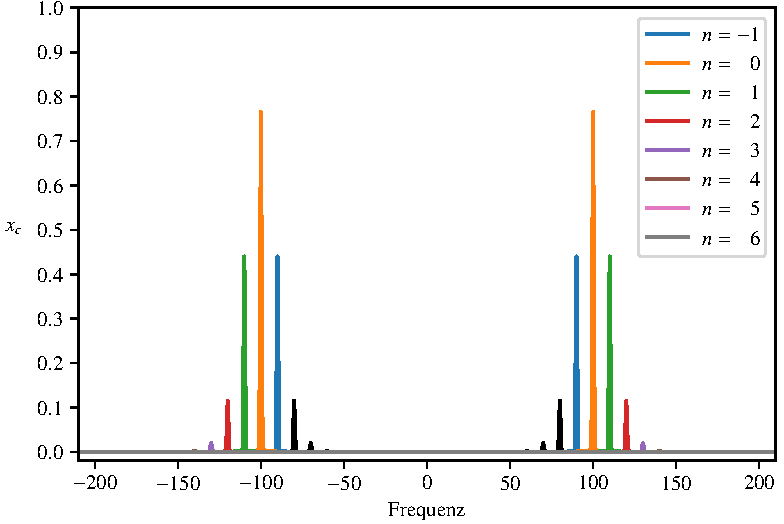
\includegraphics{papers/fm/images/fm10.pdf}
	%%% Creator: Matplotlib, PGF backend
%%
%% To include the figure in your LaTeX document, write
%%   \input{<filename>.pgf}
%%
%% Make sure the required packages are loaded in your preamble
%%   \usepackage{pgf}
%%
%% Also ensure that all the required font packages are loaded; for instance,
%% the lmodern package is sometimes necessary when using math font.
%%   \usepackage{lmodern}
%%
%% Figures using additional raster images can only be included by \input if
%% they are in the same directory as the main LaTeX file. For loading figures
%% from other directories you can use the `import` package
%%   \usepackage{import}
%%
%% and then include the figures with
%%   \import{<path to file>}{<filename>.pgf}
%%
%% Matplotlib used the following preamble
%%
\begingroup%
\makeatletter%
\begin{pgfpicture}%
\pgfpathrectangle{\pgfpointorigin}{\pgfqpoint{6.000000in}{4.000000in}}%
\pgfusepath{use as bounding box, clip}%
\begin{pgfscope}%
\pgfsetbuttcap%
\pgfsetmiterjoin%
\pgfsetlinewidth{0.000000pt}%
\definecolor{currentstroke}{rgb}{1.000000,1.000000,1.000000}%
\pgfsetstrokecolor{currentstroke}%
\pgfsetstrokeopacity{0.000000}%
\pgfsetdash{}{0pt}%
\pgfpathmoveto{\pgfqpoint{0.000000in}{0.000000in}}%
\pgfpathlineto{\pgfqpoint{6.000000in}{0.000000in}}%
\pgfpathlineto{\pgfqpoint{6.000000in}{4.000000in}}%
\pgfpathlineto{\pgfqpoint{0.000000in}{4.000000in}}%
\pgfpathlineto{\pgfqpoint{0.000000in}{0.000000in}}%
\pgfpathclose%
\pgfusepath{}%
\end{pgfscope}%
\begin{pgfscope}%
\pgfsetbuttcap%
\pgfsetmiterjoin%
\definecolor{currentfill}{rgb}{1.000000,1.000000,1.000000}%
\pgfsetfillcolor{currentfill}%
\pgfsetlinewidth{0.000000pt}%
\definecolor{currentstroke}{rgb}{0.000000,0.000000,0.000000}%
\pgfsetstrokecolor{currentstroke}%
\pgfsetstrokeopacity{0.000000}%
\pgfsetdash{}{0pt}%
\pgfpathmoveto{\pgfqpoint{0.750000in}{0.500000in}}%
\pgfpathlineto{\pgfqpoint{5.400000in}{0.500000in}}%
\pgfpathlineto{\pgfqpoint{5.400000in}{3.520000in}}%
\pgfpathlineto{\pgfqpoint{0.750000in}{3.520000in}}%
\pgfpathlineto{\pgfqpoint{0.750000in}{0.500000in}}%
\pgfpathclose%
\pgfusepath{fill}%
\end{pgfscope}%
\begin{pgfscope}%
\pgfsetbuttcap%
\pgfsetroundjoin%
\definecolor{currentfill}{rgb}{0.000000,0.000000,0.000000}%
\pgfsetfillcolor{currentfill}%
\pgfsetlinewidth{0.803000pt}%
\definecolor{currentstroke}{rgb}{0.000000,0.000000,0.000000}%
\pgfsetstrokecolor{currentstroke}%
\pgfsetdash{}{0pt}%
\pgfsys@defobject{currentmarker}{\pgfqpoint{0.000000in}{-0.048611in}}{\pgfqpoint{0.000000in}{0.000000in}}{%
\pgfpathmoveto{\pgfqpoint{0.000000in}{0.000000in}}%
\pgfpathlineto{\pgfqpoint{0.000000in}{-0.048611in}}%
\pgfusepath{stroke,fill}%
}%
\begin{pgfscope}%
\pgfsys@transformshift{0.860714in}{0.500000in}%
\pgfsys@useobject{currentmarker}{}%
\end{pgfscope}%
\end{pgfscope}%
\begin{pgfscope}%
\definecolor{textcolor}{rgb}{0.000000,0.000000,0.000000}%
\pgfsetstrokecolor{textcolor}%
\pgfsetfillcolor{textcolor}%
\pgftext[x=0.860714in,y=0.402778in,,top]{\color{textcolor}\rmfamily\fontsize{10.000000}{12.000000}\selectfont \(\displaystyle {\ensuremath{-}200}\)}%
\end{pgfscope}%
\begin{pgfscope}%
\pgfsetbuttcap%
\pgfsetroundjoin%
\definecolor{currentfill}{rgb}{0.000000,0.000000,0.000000}%
\pgfsetfillcolor{currentfill}%
\pgfsetlinewidth{0.803000pt}%
\definecolor{currentstroke}{rgb}{0.000000,0.000000,0.000000}%
\pgfsetstrokecolor{currentstroke}%
\pgfsetdash{}{0pt}%
\pgfsys@defobject{currentmarker}{\pgfqpoint{0.000000in}{-0.048611in}}{\pgfqpoint{0.000000in}{0.000000in}}{%
\pgfpathmoveto{\pgfqpoint{0.000000in}{0.000000in}}%
\pgfpathlineto{\pgfqpoint{0.000000in}{-0.048611in}}%
\pgfusepath{stroke,fill}%
}%
\begin{pgfscope}%
\pgfsys@transformshift{1.414286in}{0.500000in}%
\pgfsys@useobject{currentmarker}{}%
\end{pgfscope}%
\end{pgfscope}%
\begin{pgfscope}%
\definecolor{textcolor}{rgb}{0.000000,0.000000,0.000000}%
\pgfsetstrokecolor{textcolor}%
\pgfsetfillcolor{textcolor}%
\pgftext[x=1.414286in,y=0.402778in,,top]{\color{textcolor}\rmfamily\fontsize{10.000000}{12.000000}\selectfont \(\displaystyle {\ensuremath{-}150}\)}%
\end{pgfscope}%
\begin{pgfscope}%
\pgfsetbuttcap%
\pgfsetroundjoin%
\definecolor{currentfill}{rgb}{0.000000,0.000000,0.000000}%
\pgfsetfillcolor{currentfill}%
\pgfsetlinewidth{0.803000pt}%
\definecolor{currentstroke}{rgb}{0.000000,0.000000,0.000000}%
\pgfsetstrokecolor{currentstroke}%
\pgfsetdash{}{0pt}%
\pgfsys@defobject{currentmarker}{\pgfqpoint{0.000000in}{-0.048611in}}{\pgfqpoint{0.000000in}{0.000000in}}{%
\pgfpathmoveto{\pgfqpoint{0.000000in}{0.000000in}}%
\pgfpathlineto{\pgfqpoint{0.000000in}{-0.048611in}}%
\pgfusepath{stroke,fill}%
}%
\begin{pgfscope}%
\pgfsys@transformshift{1.967857in}{0.500000in}%
\pgfsys@useobject{currentmarker}{}%
\end{pgfscope}%
\end{pgfscope}%
\begin{pgfscope}%
\definecolor{textcolor}{rgb}{0.000000,0.000000,0.000000}%
\pgfsetstrokecolor{textcolor}%
\pgfsetfillcolor{textcolor}%
\pgftext[x=1.967857in,y=0.402778in,,top]{\color{textcolor}\rmfamily\fontsize{10.000000}{12.000000}\selectfont \(\displaystyle {\ensuremath{-}100}\)}%
\end{pgfscope}%
\begin{pgfscope}%
\pgfsetbuttcap%
\pgfsetroundjoin%
\definecolor{currentfill}{rgb}{0.000000,0.000000,0.000000}%
\pgfsetfillcolor{currentfill}%
\pgfsetlinewidth{0.803000pt}%
\definecolor{currentstroke}{rgb}{0.000000,0.000000,0.000000}%
\pgfsetstrokecolor{currentstroke}%
\pgfsetdash{}{0pt}%
\pgfsys@defobject{currentmarker}{\pgfqpoint{0.000000in}{-0.048611in}}{\pgfqpoint{0.000000in}{0.000000in}}{%
\pgfpathmoveto{\pgfqpoint{0.000000in}{0.000000in}}%
\pgfpathlineto{\pgfqpoint{0.000000in}{-0.048611in}}%
\pgfusepath{stroke,fill}%
}%
\begin{pgfscope}%
\pgfsys@transformshift{2.521429in}{0.500000in}%
\pgfsys@useobject{currentmarker}{}%
\end{pgfscope}%
\end{pgfscope}%
\begin{pgfscope}%
\definecolor{textcolor}{rgb}{0.000000,0.000000,0.000000}%
\pgfsetstrokecolor{textcolor}%
\pgfsetfillcolor{textcolor}%
\pgftext[x=2.521429in,y=0.402778in,,top]{\color{textcolor}\rmfamily\fontsize{10.000000}{12.000000}\selectfont \(\displaystyle {\ensuremath{-}50}\)}%
\end{pgfscope}%
\begin{pgfscope}%
\pgfsetbuttcap%
\pgfsetroundjoin%
\definecolor{currentfill}{rgb}{0.000000,0.000000,0.000000}%
\pgfsetfillcolor{currentfill}%
\pgfsetlinewidth{0.803000pt}%
\definecolor{currentstroke}{rgb}{0.000000,0.000000,0.000000}%
\pgfsetstrokecolor{currentstroke}%
\pgfsetdash{}{0pt}%
\pgfsys@defobject{currentmarker}{\pgfqpoint{0.000000in}{-0.048611in}}{\pgfqpoint{0.000000in}{0.000000in}}{%
\pgfpathmoveto{\pgfqpoint{0.000000in}{0.000000in}}%
\pgfpathlineto{\pgfqpoint{0.000000in}{-0.048611in}}%
\pgfusepath{stroke,fill}%
}%
\begin{pgfscope}%
\pgfsys@transformshift{3.075000in}{0.500000in}%
\pgfsys@useobject{currentmarker}{}%
\end{pgfscope}%
\end{pgfscope}%
\begin{pgfscope}%
\definecolor{textcolor}{rgb}{0.000000,0.000000,0.000000}%
\pgfsetstrokecolor{textcolor}%
\pgfsetfillcolor{textcolor}%
\pgftext[x=3.075000in,y=0.402778in,,top]{\color{textcolor}\rmfamily\fontsize{10.000000}{12.000000}\selectfont \(\displaystyle {0}\)}%
\end{pgfscope}%
\begin{pgfscope}%
\pgfsetbuttcap%
\pgfsetroundjoin%
\definecolor{currentfill}{rgb}{0.000000,0.000000,0.000000}%
\pgfsetfillcolor{currentfill}%
\pgfsetlinewidth{0.803000pt}%
\definecolor{currentstroke}{rgb}{0.000000,0.000000,0.000000}%
\pgfsetstrokecolor{currentstroke}%
\pgfsetdash{}{0pt}%
\pgfsys@defobject{currentmarker}{\pgfqpoint{0.000000in}{-0.048611in}}{\pgfqpoint{0.000000in}{0.000000in}}{%
\pgfpathmoveto{\pgfqpoint{0.000000in}{0.000000in}}%
\pgfpathlineto{\pgfqpoint{0.000000in}{-0.048611in}}%
\pgfusepath{stroke,fill}%
}%
\begin{pgfscope}%
\pgfsys@transformshift{3.628571in}{0.500000in}%
\pgfsys@useobject{currentmarker}{}%
\end{pgfscope}%
\end{pgfscope}%
\begin{pgfscope}%
\definecolor{textcolor}{rgb}{0.000000,0.000000,0.000000}%
\pgfsetstrokecolor{textcolor}%
\pgfsetfillcolor{textcolor}%
\pgftext[x=3.628571in,y=0.402778in,,top]{\color{textcolor}\rmfamily\fontsize{10.000000}{12.000000}\selectfont \(\displaystyle {50}\)}%
\end{pgfscope}%
\begin{pgfscope}%
\pgfsetbuttcap%
\pgfsetroundjoin%
\definecolor{currentfill}{rgb}{0.000000,0.000000,0.000000}%
\pgfsetfillcolor{currentfill}%
\pgfsetlinewidth{0.803000pt}%
\definecolor{currentstroke}{rgb}{0.000000,0.000000,0.000000}%
\pgfsetstrokecolor{currentstroke}%
\pgfsetdash{}{0pt}%
\pgfsys@defobject{currentmarker}{\pgfqpoint{0.000000in}{-0.048611in}}{\pgfqpoint{0.000000in}{0.000000in}}{%
\pgfpathmoveto{\pgfqpoint{0.000000in}{0.000000in}}%
\pgfpathlineto{\pgfqpoint{0.000000in}{-0.048611in}}%
\pgfusepath{stroke,fill}%
}%
\begin{pgfscope}%
\pgfsys@transformshift{4.182143in}{0.500000in}%
\pgfsys@useobject{currentmarker}{}%
\end{pgfscope}%
\end{pgfscope}%
\begin{pgfscope}%
\definecolor{textcolor}{rgb}{0.000000,0.000000,0.000000}%
\pgfsetstrokecolor{textcolor}%
\pgfsetfillcolor{textcolor}%
\pgftext[x=4.182143in,y=0.402778in,,top]{\color{textcolor}\rmfamily\fontsize{10.000000}{12.000000}\selectfont \(\displaystyle {100}\)}%
\end{pgfscope}%
\begin{pgfscope}%
\pgfsetbuttcap%
\pgfsetroundjoin%
\definecolor{currentfill}{rgb}{0.000000,0.000000,0.000000}%
\pgfsetfillcolor{currentfill}%
\pgfsetlinewidth{0.803000pt}%
\definecolor{currentstroke}{rgb}{0.000000,0.000000,0.000000}%
\pgfsetstrokecolor{currentstroke}%
\pgfsetdash{}{0pt}%
\pgfsys@defobject{currentmarker}{\pgfqpoint{0.000000in}{-0.048611in}}{\pgfqpoint{0.000000in}{0.000000in}}{%
\pgfpathmoveto{\pgfqpoint{0.000000in}{0.000000in}}%
\pgfpathlineto{\pgfqpoint{0.000000in}{-0.048611in}}%
\pgfusepath{stroke,fill}%
}%
\begin{pgfscope}%
\pgfsys@transformshift{4.735714in}{0.500000in}%
\pgfsys@useobject{currentmarker}{}%
\end{pgfscope}%
\end{pgfscope}%
\begin{pgfscope}%
\definecolor{textcolor}{rgb}{0.000000,0.000000,0.000000}%
\pgfsetstrokecolor{textcolor}%
\pgfsetfillcolor{textcolor}%
\pgftext[x=4.735714in,y=0.402778in,,top]{\color{textcolor}\rmfamily\fontsize{10.000000}{12.000000}\selectfont \(\displaystyle {150}\)}%
\end{pgfscope}%
\begin{pgfscope}%
\pgfsetbuttcap%
\pgfsetroundjoin%
\definecolor{currentfill}{rgb}{0.000000,0.000000,0.000000}%
\pgfsetfillcolor{currentfill}%
\pgfsetlinewidth{0.803000pt}%
\definecolor{currentstroke}{rgb}{0.000000,0.000000,0.000000}%
\pgfsetstrokecolor{currentstroke}%
\pgfsetdash{}{0pt}%
\pgfsys@defobject{currentmarker}{\pgfqpoint{0.000000in}{-0.048611in}}{\pgfqpoint{0.000000in}{0.000000in}}{%
\pgfpathmoveto{\pgfqpoint{0.000000in}{0.000000in}}%
\pgfpathlineto{\pgfqpoint{0.000000in}{-0.048611in}}%
\pgfusepath{stroke,fill}%
}%
\begin{pgfscope}%
\pgfsys@transformshift{5.289286in}{0.500000in}%
\pgfsys@useobject{currentmarker}{}%
\end{pgfscope}%
\end{pgfscope}%
\begin{pgfscope}%
\definecolor{textcolor}{rgb}{0.000000,0.000000,0.000000}%
\pgfsetstrokecolor{textcolor}%
\pgfsetfillcolor{textcolor}%
\pgftext[x=5.289286in,y=0.402778in,,top]{\color{textcolor}\rmfamily\fontsize{10.000000}{12.000000}\selectfont \(\displaystyle {200}\)}%
\end{pgfscope}%
\begin{pgfscope}%
\definecolor{textcolor}{rgb}{0.000000,0.000000,0.000000}%
\pgfsetstrokecolor{textcolor}%
\pgfsetfillcolor{textcolor}%
\pgftext[x=3.075000in,y=0.223766in,,top]{\color{textcolor}\rmfamily\fontsize{10.000000}{12.000000}\selectfont Frequenz}%
\end{pgfscope}%
\begin{pgfscope}%
\pgfsetbuttcap%
\pgfsetroundjoin%
\definecolor{currentfill}{rgb}{0.000000,0.000000,0.000000}%
\pgfsetfillcolor{currentfill}%
\pgfsetlinewidth{0.803000pt}%
\definecolor{currentstroke}{rgb}{0.000000,0.000000,0.000000}%
\pgfsetstrokecolor{currentstroke}%
\pgfsetdash{}{0pt}%
\pgfsys@defobject{currentmarker}{\pgfqpoint{-0.048611in}{0.000000in}}{\pgfqpoint{-0.000000in}{0.000000in}}{%
\pgfpathmoveto{\pgfqpoint{-0.000000in}{0.000000in}}%
\pgfpathlineto{\pgfqpoint{-0.048611in}{0.000000in}}%
\pgfusepath{stroke,fill}%
}%
\begin{pgfscope}%
\pgfsys@transformshift{0.750000in}{0.559216in}%
\pgfsys@useobject{currentmarker}{}%
\end{pgfscope}%
\end{pgfscope}%
\begin{pgfscope}%
\definecolor{textcolor}{rgb}{0.000000,0.000000,0.000000}%
\pgfsetstrokecolor{textcolor}%
\pgfsetfillcolor{textcolor}%
\pgftext[x=0.475308in, y=0.510990in, left, base]{\color{textcolor}\rmfamily\fontsize{10.000000}{12.000000}\selectfont \(\displaystyle {0.0}\)}%
\end{pgfscope}%
\begin{pgfscope}%
\pgfsetbuttcap%
\pgfsetroundjoin%
\definecolor{currentfill}{rgb}{0.000000,0.000000,0.000000}%
\pgfsetfillcolor{currentfill}%
\pgfsetlinewidth{0.803000pt}%
\definecolor{currentstroke}{rgb}{0.000000,0.000000,0.000000}%
\pgfsetstrokecolor{currentstroke}%
\pgfsetdash{}{0pt}%
\pgfsys@defobject{currentmarker}{\pgfqpoint{-0.048611in}{0.000000in}}{\pgfqpoint{-0.000000in}{0.000000in}}{%
\pgfpathmoveto{\pgfqpoint{-0.000000in}{0.000000in}}%
\pgfpathlineto{\pgfqpoint{-0.048611in}{0.000000in}}%
\pgfusepath{stroke,fill}%
}%
\begin{pgfscope}%
\pgfsys@transformshift{0.750000in}{0.855294in}%
\pgfsys@useobject{currentmarker}{}%
\end{pgfscope}%
\end{pgfscope}%
\begin{pgfscope}%
\definecolor{textcolor}{rgb}{0.000000,0.000000,0.000000}%
\pgfsetstrokecolor{textcolor}%
\pgfsetfillcolor{textcolor}%
\pgftext[x=0.475308in, y=0.807069in, left, base]{\color{textcolor}\rmfamily\fontsize{10.000000}{12.000000}\selectfont \(\displaystyle {0.1}\)}%
\end{pgfscope}%
\begin{pgfscope}%
\pgfsetbuttcap%
\pgfsetroundjoin%
\definecolor{currentfill}{rgb}{0.000000,0.000000,0.000000}%
\pgfsetfillcolor{currentfill}%
\pgfsetlinewidth{0.803000pt}%
\definecolor{currentstroke}{rgb}{0.000000,0.000000,0.000000}%
\pgfsetstrokecolor{currentstroke}%
\pgfsetdash{}{0pt}%
\pgfsys@defobject{currentmarker}{\pgfqpoint{-0.048611in}{0.000000in}}{\pgfqpoint{-0.000000in}{0.000000in}}{%
\pgfpathmoveto{\pgfqpoint{-0.000000in}{0.000000in}}%
\pgfpathlineto{\pgfqpoint{-0.048611in}{0.000000in}}%
\pgfusepath{stroke,fill}%
}%
\begin{pgfscope}%
\pgfsys@transformshift{0.750000in}{1.151373in}%
\pgfsys@useobject{currentmarker}{}%
\end{pgfscope}%
\end{pgfscope}%
\begin{pgfscope}%
\definecolor{textcolor}{rgb}{0.000000,0.000000,0.000000}%
\pgfsetstrokecolor{textcolor}%
\pgfsetfillcolor{textcolor}%
\pgftext[x=0.475308in, y=1.103147in, left, base]{\color{textcolor}\rmfamily\fontsize{10.000000}{12.000000}\selectfont \(\displaystyle {0.2}\)}%
\end{pgfscope}%
\begin{pgfscope}%
\pgfsetbuttcap%
\pgfsetroundjoin%
\definecolor{currentfill}{rgb}{0.000000,0.000000,0.000000}%
\pgfsetfillcolor{currentfill}%
\pgfsetlinewidth{0.803000pt}%
\definecolor{currentstroke}{rgb}{0.000000,0.000000,0.000000}%
\pgfsetstrokecolor{currentstroke}%
\pgfsetdash{}{0pt}%
\pgfsys@defobject{currentmarker}{\pgfqpoint{-0.048611in}{0.000000in}}{\pgfqpoint{-0.000000in}{0.000000in}}{%
\pgfpathmoveto{\pgfqpoint{-0.000000in}{0.000000in}}%
\pgfpathlineto{\pgfqpoint{-0.048611in}{0.000000in}}%
\pgfusepath{stroke,fill}%
}%
\begin{pgfscope}%
\pgfsys@transformshift{0.750000in}{1.447451in}%
\pgfsys@useobject{currentmarker}{}%
\end{pgfscope}%
\end{pgfscope}%
\begin{pgfscope}%
\definecolor{textcolor}{rgb}{0.000000,0.000000,0.000000}%
\pgfsetstrokecolor{textcolor}%
\pgfsetfillcolor{textcolor}%
\pgftext[x=0.475308in, y=1.399226in, left, base]{\color{textcolor}\rmfamily\fontsize{10.000000}{12.000000}\selectfont \(\displaystyle {0.3}\)}%
\end{pgfscope}%
\begin{pgfscope}%
\pgfsetbuttcap%
\pgfsetroundjoin%
\definecolor{currentfill}{rgb}{0.000000,0.000000,0.000000}%
\pgfsetfillcolor{currentfill}%
\pgfsetlinewidth{0.803000pt}%
\definecolor{currentstroke}{rgb}{0.000000,0.000000,0.000000}%
\pgfsetstrokecolor{currentstroke}%
\pgfsetdash{}{0pt}%
\pgfsys@defobject{currentmarker}{\pgfqpoint{-0.048611in}{0.000000in}}{\pgfqpoint{-0.000000in}{0.000000in}}{%
\pgfpathmoveto{\pgfqpoint{-0.000000in}{0.000000in}}%
\pgfpathlineto{\pgfqpoint{-0.048611in}{0.000000in}}%
\pgfusepath{stroke,fill}%
}%
\begin{pgfscope}%
\pgfsys@transformshift{0.750000in}{1.743529in}%
\pgfsys@useobject{currentmarker}{}%
\end{pgfscope}%
\end{pgfscope}%
\begin{pgfscope}%
\definecolor{textcolor}{rgb}{0.000000,0.000000,0.000000}%
\pgfsetstrokecolor{textcolor}%
\pgfsetfillcolor{textcolor}%
\pgftext[x=0.475308in, y=1.695304in, left, base]{\color{textcolor}\rmfamily\fontsize{10.000000}{12.000000}\selectfont \(\displaystyle {0.4}\)}%
\end{pgfscope}%
\begin{pgfscope}%
\pgfsetbuttcap%
\pgfsetroundjoin%
\definecolor{currentfill}{rgb}{0.000000,0.000000,0.000000}%
\pgfsetfillcolor{currentfill}%
\pgfsetlinewidth{0.803000pt}%
\definecolor{currentstroke}{rgb}{0.000000,0.000000,0.000000}%
\pgfsetstrokecolor{currentstroke}%
\pgfsetdash{}{0pt}%
\pgfsys@defobject{currentmarker}{\pgfqpoint{-0.048611in}{0.000000in}}{\pgfqpoint{-0.000000in}{0.000000in}}{%
\pgfpathmoveto{\pgfqpoint{-0.000000in}{0.000000in}}%
\pgfpathlineto{\pgfqpoint{-0.048611in}{0.000000in}}%
\pgfusepath{stroke,fill}%
}%
\begin{pgfscope}%
\pgfsys@transformshift{0.750000in}{2.039608in}%
\pgfsys@useobject{currentmarker}{}%
\end{pgfscope}%
\end{pgfscope}%
\begin{pgfscope}%
\definecolor{textcolor}{rgb}{0.000000,0.000000,0.000000}%
\pgfsetstrokecolor{textcolor}%
\pgfsetfillcolor{textcolor}%
\pgftext[x=0.475308in, y=1.991383in, left, base]{\color{textcolor}\rmfamily\fontsize{10.000000}{12.000000}\selectfont \(\displaystyle {0.5}\)}%
\end{pgfscope}%
\begin{pgfscope}%
\pgfsetbuttcap%
\pgfsetroundjoin%
\definecolor{currentfill}{rgb}{0.000000,0.000000,0.000000}%
\pgfsetfillcolor{currentfill}%
\pgfsetlinewidth{0.803000pt}%
\definecolor{currentstroke}{rgb}{0.000000,0.000000,0.000000}%
\pgfsetstrokecolor{currentstroke}%
\pgfsetdash{}{0pt}%
\pgfsys@defobject{currentmarker}{\pgfqpoint{-0.048611in}{0.000000in}}{\pgfqpoint{-0.000000in}{0.000000in}}{%
\pgfpathmoveto{\pgfqpoint{-0.000000in}{0.000000in}}%
\pgfpathlineto{\pgfqpoint{-0.048611in}{0.000000in}}%
\pgfusepath{stroke,fill}%
}%
\begin{pgfscope}%
\pgfsys@transformshift{0.750000in}{2.335686in}%
\pgfsys@useobject{currentmarker}{}%
\end{pgfscope}%
\end{pgfscope}%
\begin{pgfscope}%
\definecolor{textcolor}{rgb}{0.000000,0.000000,0.000000}%
\pgfsetstrokecolor{textcolor}%
\pgfsetfillcolor{textcolor}%
\pgftext[x=0.475308in, y=2.287461in, left, base]{\color{textcolor}\rmfamily\fontsize{10.000000}{12.000000}\selectfont \(\displaystyle {0.6}\)}%
\end{pgfscope}%
\begin{pgfscope}%
\pgfsetbuttcap%
\pgfsetroundjoin%
\definecolor{currentfill}{rgb}{0.000000,0.000000,0.000000}%
\pgfsetfillcolor{currentfill}%
\pgfsetlinewidth{0.803000pt}%
\definecolor{currentstroke}{rgb}{0.000000,0.000000,0.000000}%
\pgfsetstrokecolor{currentstroke}%
\pgfsetdash{}{0pt}%
\pgfsys@defobject{currentmarker}{\pgfqpoint{-0.048611in}{0.000000in}}{\pgfqpoint{-0.000000in}{0.000000in}}{%
\pgfpathmoveto{\pgfqpoint{-0.000000in}{0.000000in}}%
\pgfpathlineto{\pgfqpoint{-0.048611in}{0.000000in}}%
\pgfusepath{stroke,fill}%
}%
\begin{pgfscope}%
\pgfsys@transformshift{0.750000in}{2.631765in}%
\pgfsys@useobject{currentmarker}{}%
\end{pgfscope}%
\end{pgfscope}%
\begin{pgfscope}%
\definecolor{textcolor}{rgb}{0.000000,0.000000,0.000000}%
\pgfsetstrokecolor{textcolor}%
\pgfsetfillcolor{textcolor}%
\pgftext[x=0.475308in, y=2.583539in, left, base]{\color{textcolor}\rmfamily\fontsize{10.000000}{12.000000}\selectfont \(\displaystyle {0.7}\)}%
\end{pgfscope}%
\begin{pgfscope}%
\pgfsetbuttcap%
\pgfsetroundjoin%
\definecolor{currentfill}{rgb}{0.000000,0.000000,0.000000}%
\pgfsetfillcolor{currentfill}%
\pgfsetlinewidth{0.803000pt}%
\definecolor{currentstroke}{rgb}{0.000000,0.000000,0.000000}%
\pgfsetstrokecolor{currentstroke}%
\pgfsetdash{}{0pt}%
\pgfsys@defobject{currentmarker}{\pgfqpoint{-0.048611in}{0.000000in}}{\pgfqpoint{-0.000000in}{0.000000in}}{%
\pgfpathmoveto{\pgfqpoint{-0.000000in}{0.000000in}}%
\pgfpathlineto{\pgfqpoint{-0.048611in}{0.000000in}}%
\pgfusepath{stroke,fill}%
}%
\begin{pgfscope}%
\pgfsys@transformshift{0.750000in}{2.927843in}%
\pgfsys@useobject{currentmarker}{}%
\end{pgfscope}%
\end{pgfscope}%
\begin{pgfscope}%
\definecolor{textcolor}{rgb}{0.000000,0.000000,0.000000}%
\pgfsetstrokecolor{textcolor}%
\pgfsetfillcolor{textcolor}%
\pgftext[x=0.475308in, y=2.879618in, left, base]{\color{textcolor}\rmfamily\fontsize{10.000000}{12.000000}\selectfont \(\displaystyle {0.8}\)}%
\end{pgfscope}%
\begin{pgfscope}%
\pgfsetbuttcap%
\pgfsetroundjoin%
\definecolor{currentfill}{rgb}{0.000000,0.000000,0.000000}%
\pgfsetfillcolor{currentfill}%
\pgfsetlinewidth{0.803000pt}%
\definecolor{currentstroke}{rgb}{0.000000,0.000000,0.000000}%
\pgfsetstrokecolor{currentstroke}%
\pgfsetdash{}{0pt}%
\pgfsys@defobject{currentmarker}{\pgfqpoint{-0.048611in}{0.000000in}}{\pgfqpoint{-0.000000in}{0.000000in}}{%
\pgfpathmoveto{\pgfqpoint{-0.000000in}{0.000000in}}%
\pgfpathlineto{\pgfqpoint{-0.048611in}{0.000000in}}%
\pgfusepath{stroke,fill}%
}%
\begin{pgfscope}%
\pgfsys@transformshift{0.750000in}{3.223922in}%
\pgfsys@useobject{currentmarker}{}%
\end{pgfscope}%
\end{pgfscope}%
\begin{pgfscope}%
\definecolor{textcolor}{rgb}{0.000000,0.000000,0.000000}%
\pgfsetstrokecolor{textcolor}%
\pgfsetfillcolor{textcolor}%
\pgftext[x=0.475308in, y=3.175696in, left, base]{\color{textcolor}\rmfamily\fontsize{10.000000}{12.000000}\selectfont \(\displaystyle {0.9}\)}%
\end{pgfscope}%
\begin{pgfscope}%
\pgfsetbuttcap%
\pgfsetroundjoin%
\definecolor{currentfill}{rgb}{0.000000,0.000000,0.000000}%
\pgfsetfillcolor{currentfill}%
\pgfsetlinewidth{0.803000pt}%
\definecolor{currentstroke}{rgb}{0.000000,0.000000,0.000000}%
\pgfsetstrokecolor{currentstroke}%
\pgfsetdash{}{0pt}%
\pgfsys@defobject{currentmarker}{\pgfqpoint{-0.048611in}{0.000000in}}{\pgfqpoint{-0.000000in}{0.000000in}}{%
\pgfpathmoveto{\pgfqpoint{-0.000000in}{0.000000in}}%
\pgfpathlineto{\pgfqpoint{-0.048611in}{0.000000in}}%
\pgfusepath{stroke,fill}%
}%
\begin{pgfscope}%
\pgfsys@transformshift{0.750000in}{3.520000in}%
\pgfsys@useobject{currentmarker}{}%
\end{pgfscope}%
\end{pgfscope}%
\begin{pgfscope}%
\definecolor{textcolor}{rgb}{0.000000,0.000000,0.000000}%
\pgfsetstrokecolor{textcolor}%
\pgfsetfillcolor{textcolor}%
\pgftext[x=0.475308in, y=3.471775in, left, base]{\color{textcolor}\rmfamily\fontsize{10.000000}{12.000000}\selectfont \(\displaystyle {1.0}\)}%
\end{pgfscope}%
\begin{pgfscope}%
\definecolor{textcolor}{rgb}{0.000000,0.000000,0.000000}%
\pgfsetstrokecolor{textcolor}%
\pgfsetfillcolor{textcolor}%
\pgftext[x=0.319753in,y=2.010000in,,bottom,rotate=00.000000]{\color{textcolor}\rmfamily\fontsize{10.000000}{12.000000}\selectfont \(\displaystyle x_c\)}%
\end{pgfscope}%
\begin{pgfscope}%
\pgfpathrectangle{\pgfqpoint{0.750000in}{0.500000in}}{\pgfqpoint{4.650000in}{3.020000in}}%
\pgfusepath{clip}%
\pgfsetrectcap%
\pgfsetroundjoin%
\pgfsetlinewidth{1.505625pt}%
\definecolor{currentstroke}{rgb}{0.000000,0.000000,0.000000}%
\pgfsetstrokecolor{currentstroke}%
\pgfsetdash{}{0pt}%
\pgfpathmoveto{\pgfqpoint{3.075000in}{0.559216in}}%
\pgfpathlineto{\pgfqpoint{5.413889in}{0.559216in}}%
\pgfpathmoveto{\pgfqpoint{5.413889in}{0.559216in}}%
\pgfpathlineto{\pgfqpoint{0.736111in}{0.559216in}}%
\pgfpathmoveto{\pgfqpoint{0.736111in}{0.559216in}}%
\pgfpathlineto{\pgfqpoint{3.063929in}{0.559216in}}%
\pgfpathlineto{\pgfqpoint{3.063929in}{0.559216in}}%
\pgfusepath{stroke}%
\end{pgfscope}%
\begin{pgfscope}%
\pgfpathrectangle{\pgfqpoint{0.750000in}{0.500000in}}{\pgfqpoint{4.650000in}{3.020000in}}%
\pgfusepath{clip}%
\pgfsetrectcap%
\pgfsetroundjoin%
\pgfsetlinewidth{1.505625pt}%
\definecolor{currentstroke}{rgb}{0.000000,0.000000,0.000000}%
\pgfsetstrokecolor{currentstroke}%
\pgfsetdash{}{0pt}%
\pgfpathmoveto{\pgfqpoint{3.075000in}{0.559216in}}%
\pgfpathlineto{\pgfqpoint{5.413889in}{0.559216in}}%
\pgfpathmoveto{\pgfqpoint{5.413889in}{0.559216in}}%
\pgfpathlineto{\pgfqpoint{0.736111in}{0.559216in}}%
\pgfpathmoveto{\pgfqpoint{0.736111in}{0.559216in}}%
\pgfpathlineto{\pgfqpoint{3.063929in}{0.559216in}}%
\pgfpathlineto{\pgfqpoint{3.063929in}{0.559216in}}%
\pgfusepath{stroke}%
\end{pgfscope}%
\begin{pgfscope}%
\pgfpathrectangle{\pgfqpoint{0.750000in}{0.500000in}}{\pgfqpoint{4.650000in}{3.020000in}}%
\pgfusepath{clip}%
\pgfsetrectcap%
\pgfsetroundjoin%
\pgfsetlinewidth{1.505625pt}%
\definecolor{currentstroke}{rgb}{0.000000,0.000000,0.000000}%
\pgfsetstrokecolor{currentstroke}%
\pgfsetdash{}{0pt}%
\pgfpathmoveto{\pgfqpoint{3.075000in}{0.559217in}}%
\pgfpathlineto{\pgfqpoint{3.728214in}{0.559259in}}%
\pgfpathlineto{\pgfqpoint{3.739286in}{0.566548in}}%
\pgfpathlineto{\pgfqpoint{3.750357in}{0.559260in}}%
\pgfpathlineto{\pgfqpoint{4.536429in}{0.559216in}}%
\pgfpathlineto{\pgfqpoint{5.413889in}{0.559216in}}%
\pgfpathmoveto{\pgfqpoint{5.413889in}{0.559216in}}%
\pgfpathlineto{\pgfqpoint{0.736111in}{0.559216in}}%
\pgfpathmoveto{\pgfqpoint{0.736111in}{0.559216in}}%
\pgfpathlineto{\pgfqpoint{2.399643in}{0.559260in}}%
\pgfpathlineto{\pgfqpoint{2.410714in}{0.566548in}}%
\pgfpathlineto{\pgfqpoint{2.421786in}{0.559259in}}%
\pgfpathlineto{\pgfqpoint{3.063929in}{0.559217in}}%
\pgfpathlineto{\pgfqpoint{3.063929in}{0.559217in}}%
\pgfusepath{stroke}%
\end{pgfscope}%
\begin{pgfscope}%
\pgfpathrectangle{\pgfqpoint{0.750000in}{0.500000in}}{\pgfqpoint{4.650000in}{3.020000in}}%
\pgfusepath{clip}%
\pgfsetrectcap%
\pgfsetroundjoin%
\pgfsetlinewidth{1.505625pt}%
\definecolor{currentstroke}{rgb}{0.000000,0.000000,0.000000}%
\pgfsetstrokecolor{currentstroke}%
\pgfsetdash{}{0pt}%
\pgfpathmoveto{\pgfqpoint{3.075000in}{0.559227in}}%
\pgfpathlineto{\pgfqpoint{3.838929in}{0.559621in}}%
\pgfpathlineto{\pgfqpoint{3.850000in}{0.617136in}}%
\pgfpathlineto{\pgfqpoint{3.861071in}{0.559622in}}%
\pgfpathlineto{\pgfqpoint{3.960714in}{0.559254in}}%
\pgfpathlineto{\pgfqpoint{5.413889in}{0.559218in}}%
\pgfpathmoveto{\pgfqpoint{5.413889in}{0.559216in}}%
\pgfpathlineto{\pgfqpoint{0.736111in}{0.559216in}}%
\pgfpathmoveto{\pgfqpoint{0.736111in}{0.559218in}}%
\pgfpathlineto{\pgfqpoint{2.288929in}{0.559622in}}%
\pgfpathlineto{\pgfqpoint{2.300000in}{0.617136in}}%
\pgfpathlineto{\pgfqpoint{2.311071in}{0.559621in}}%
\pgfpathlineto{\pgfqpoint{2.410714in}{0.559259in}}%
\pgfpathlineto{\pgfqpoint{3.063929in}{0.559227in}}%
\pgfpathlineto{\pgfqpoint{3.063929in}{0.559227in}}%
\pgfusepath{stroke}%
\end{pgfscope}%
\begin{pgfscope}%
\pgfpathrectangle{\pgfqpoint{0.750000in}{0.500000in}}{\pgfqpoint{4.650000in}{3.020000in}}%
\pgfusepath{clip}%
\pgfsetrectcap%
\pgfsetroundjoin%
\pgfsetlinewidth{1.505625pt}%
\definecolor{currentstroke}{rgb}{0.000000,0.000000,0.000000}%
\pgfsetstrokecolor{currentstroke}%
\pgfsetdash{}{0pt}%
\pgfpathmoveto{\pgfqpoint{3.075000in}{0.559280in}}%
\pgfpathlineto{\pgfqpoint{3.938571in}{0.560585in}}%
\pgfpathlineto{\pgfqpoint{3.949643in}{0.561930in}}%
\pgfpathlineto{\pgfqpoint{3.960714in}{0.899398in}}%
\pgfpathlineto{\pgfqpoint{3.971786in}{0.561946in}}%
\pgfpathlineto{\pgfqpoint{3.993929in}{0.560112in}}%
\pgfpathlineto{\pgfqpoint{4.093571in}{0.559430in}}%
\pgfpathlineto{\pgfqpoint{5.200714in}{0.559233in}}%
\pgfpathlineto{\pgfqpoint{5.413889in}{0.559230in}}%
\pgfpathmoveto{\pgfqpoint{5.413889in}{0.559216in}}%
\pgfpathlineto{\pgfqpoint{0.736111in}{0.559216in}}%
\pgfpathmoveto{\pgfqpoint{0.736111in}{0.559230in}}%
\pgfpathlineto{\pgfqpoint{2.167143in}{0.560568in}}%
\pgfpathlineto{\pgfqpoint{2.178214in}{0.561946in}}%
\pgfpathlineto{\pgfqpoint{2.189286in}{0.899398in}}%
\pgfpathlineto{\pgfqpoint{2.200357in}{0.561930in}}%
\pgfpathlineto{\pgfqpoint{2.222500in}{0.560135in}}%
\pgfpathlineto{\pgfqpoint{2.322143in}{0.559457in}}%
\pgfpathlineto{\pgfqpoint{3.063929in}{0.559280in}}%
\pgfpathlineto{\pgfqpoint{3.063929in}{0.559280in}}%
\pgfusepath{stroke}%
\end{pgfscope}%
\begin{pgfscope}%
\pgfpathrectangle{\pgfqpoint{0.750000in}{0.500000in}}{\pgfqpoint{4.650000in}{3.020000in}}%
\pgfusepath{clip}%
\pgfsetrectcap%
\pgfsetroundjoin%
\pgfsetlinewidth{1.505625pt}%
\definecolor{currentstroke}{rgb}{0.121569,0.466667,0.705882}%
\pgfsetstrokecolor{currentstroke}%
\pgfsetdash{}{0pt}%
\pgfpathmoveto{\pgfqpoint{3.075000in}{0.559369in}}%
\pgfpathlineto{\pgfqpoint{3.993929in}{0.560869in}}%
\pgfpathlineto{\pgfqpoint{4.038214in}{0.563093in}}%
\pgfpathlineto{\pgfqpoint{4.049286in}{0.565032in}}%
\pgfpathlineto{\pgfqpoint{4.060357in}{0.570817in}}%
\pgfpathlineto{\pgfqpoint{4.071429in}{1.861917in}}%
\pgfpathlineto{\pgfqpoint{4.082500in}{0.571068in}}%
\pgfpathlineto{\pgfqpoint{4.093571in}{0.565125in}}%
\pgfpathlineto{\pgfqpoint{4.115714in}{0.562174in}}%
\pgfpathlineto{\pgfqpoint{4.171071in}{0.560540in}}%
\pgfpathlineto{\pgfqpoint{4.370357in}{0.559671in}}%
\pgfpathlineto{\pgfqpoint{5.413889in}{0.559331in}}%
\pgfpathmoveto{\pgfqpoint{5.413889in}{0.559222in}}%
\pgfpathlineto{\pgfqpoint{0.736111in}{0.559222in}}%
\pgfpathmoveto{\pgfqpoint{0.736111in}{0.559331in}}%
\pgfpathlineto{\pgfqpoint{2.001071in}{0.560913in}}%
\pgfpathlineto{\pgfqpoint{2.045357in}{0.563156in}}%
\pgfpathlineto{\pgfqpoint{2.056429in}{0.565125in}}%
\pgfpathlineto{\pgfqpoint{2.067500in}{0.571068in}}%
\pgfpathlineto{\pgfqpoint{2.078571in}{1.861917in}}%
\pgfpathlineto{\pgfqpoint{2.089643in}{0.570817in}}%
\pgfpathlineto{\pgfqpoint{2.100714in}{0.565032in}}%
\pgfpathlineto{\pgfqpoint{2.122857in}{0.562121in}}%
\pgfpathlineto{\pgfqpoint{2.178214in}{0.560498in}}%
\pgfpathlineto{\pgfqpoint{2.377500in}{0.559633in}}%
\pgfpathlineto{\pgfqpoint{3.063929in}{0.559369in}}%
\pgfpathlineto{\pgfqpoint{3.063929in}{0.559369in}}%
\pgfusepath{stroke}%
\end{pgfscope}%
\begin{pgfscope}%
\pgfpathrectangle{\pgfqpoint{0.750000in}{0.500000in}}{\pgfqpoint{4.650000in}{3.020000in}}%
\pgfusepath{clip}%
\pgfsetrectcap%
\pgfsetroundjoin%
\pgfsetlinewidth{1.505625pt}%
\definecolor{currentstroke}{rgb}{1.000000,0.498039,0.054902}%
\pgfsetstrokecolor{currentstroke}%
\pgfsetdash{}{0pt}%
\pgfpathmoveto{\pgfqpoint{3.075000in}{0.559216in}}%
\pgfpathlineto{\pgfqpoint{4.060357in}{0.561153in}}%
\pgfpathlineto{\pgfqpoint{4.126786in}{0.563621in}}%
\pgfpathlineto{\pgfqpoint{4.148929in}{0.566627in}}%
\pgfpathlineto{\pgfqpoint{4.160000in}{0.570372in}}%
\pgfpathlineto{\pgfqpoint{4.171071in}{0.581532in}}%
\pgfpathlineto{\pgfqpoint{4.182143in}{2.824315in}}%
\pgfpathlineto{\pgfqpoint{4.193214in}{0.582212in}}%
\pgfpathlineto{\pgfqpoint{4.204286in}{0.570712in}}%
\pgfpathlineto{\pgfqpoint{4.215357in}{0.566904in}}%
\pgfpathlineto{\pgfqpoint{4.237500in}{0.563866in}}%
\pgfpathlineto{\pgfqpoint{4.292857in}{0.561591in}}%
\pgfpathlineto{\pgfqpoint{4.436786in}{0.560303in}}%
\pgfpathlineto{\pgfqpoint{5.034643in}{0.559592in}}%
\pgfpathlineto{\pgfqpoint{5.413889in}{0.559492in}}%
\pgfpathmoveto{\pgfqpoint{5.413889in}{0.559230in}}%
\pgfpathlineto{\pgfqpoint{0.736111in}{0.559230in}}%
\pgfpathmoveto{\pgfqpoint{0.736111in}{0.559492in}}%
\pgfpathlineto{\pgfqpoint{1.835000in}{0.561212in}}%
\pgfpathlineto{\pgfqpoint{1.912500in}{0.563866in}}%
\pgfpathlineto{\pgfqpoint{1.934643in}{0.566904in}}%
\pgfpathlineto{\pgfqpoint{1.945714in}{0.570712in}}%
\pgfpathlineto{\pgfqpoint{1.956786in}{0.582212in}}%
\pgfpathlineto{\pgfqpoint{1.967857in}{2.824315in}}%
\pgfpathlineto{\pgfqpoint{1.978929in}{0.581532in}}%
\pgfpathlineto{\pgfqpoint{1.990000in}{0.570372in}}%
\pgfpathlineto{\pgfqpoint{2.001071in}{0.566627in}}%
\pgfpathlineto{\pgfqpoint{2.023214in}{0.563621in}}%
\pgfpathlineto{\pgfqpoint{2.078571in}{0.561360in}}%
\pgfpathlineto{\pgfqpoint{2.222500in}{0.560072in}}%
\pgfpathlineto{\pgfqpoint{2.820357in}{0.559326in}}%
\pgfpathlineto{\pgfqpoint{3.063929in}{0.559220in}}%
\pgfpathlineto{\pgfqpoint{3.063929in}{0.559220in}}%
\pgfusepath{stroke}%
\end{pgfscope}%
\begin{pgfscope}%
\pgfpathrectangle{\pgfqpoint{0.750000in}{0.500000in}}{\pgfqpoint{4.650000in}{3.020000in}}%
\pgfusepath{clip}%
\pgfsetrectcap%
\pgfsetroundjoin%
\pgfsetlinewidth{1.505625pt}%
\definecolor{currentstroke}{rgb}{0.172549,0.627451,0.172549}%
\pgfsetstrokecolor{currentstroke}%
\pgfsetdash{}{0pt}%
\pgfpathmoveto{\pgfqpoint{3.075000in}{0.559369in}}%
\pgfpathlineto{\pgfqpoint{4.193214in}{0.560786in}}%
\pgfpathlineto{\pgfqpoint{4.248571in}{0.562769in}}%
\pgfpathlineto{\pgfqpoint{4.270714in}{0.566322in}}%
\pgfpathlineto{\pgfqpoint{4.281786in}{0.573370in}}%
\pgfpathlineto{\pgfqpoint{4.292857in}{1.861831in}}%
\pgfpathlineto{\pgfqpoint{4.303929in}{0.573726in}}%
\pgfpathlineto{\pgfqpoint{4.315000in}{0.566441in}}%
\pgfpathlineto{\pgfqpoint{4.337143in}{0.562828in}}%
\pgfpathlineto{\pgfqpoint{4.381429in}{0.561030in}}%
\pgfpathlineto{\pgfqpoint{4.525357in}{0.559919in}}%
\pgfpathlineto{\pgfqpoint{5.256071in}{0.559400in}}%
\pgfpathlineto{\pgfqpoint{5.413889in}{0.559377in}}%
\pgfpathmoveto{\pgfqpoint{5.413889in}{0.559223in}}%
\pgfpathlineto{\pgfqpoint{0.736111in}{0.559223in}}%
\pgfpathmoveto{\pgfqpoint{0.736111in}{0.559377in}}%
\pgfpathlineto{\pgfqpoint{1.768571in}{0.561030in}}%
\pgfpathlineto{\pgfqpoint{1.812857in}{0.562828in}}%
\pgfpathlineto{\pgfqpoint{1.835000in}{0.566441in}}%
\pgfpathlineto{\pgfqpoint{1.846071in}{0.573726in}}%
\pgfpathlineto{\pgfqpoint{1.857143in}{1.861831in}}%
\pgfpathlineto{\pgfqpoint{1.868214in}{0.573370in}}%
\pgfpathlineto{\pgfqpoint{1.879286in}{0.566322in}}%
\pgfpathlineto{\pgfqpoint{1.901429in}{0.562769in}}%
\pgfpathlineto{\pgfqpoint{1.945714in}{0.560985in}}%
\pgfpathlineto{\pgfqpoint{2.089643in}{0.559879in}}%
\pgfpathlineto{\pgfqpoint{2.820357in}{0.559382in}}%
\pgfpathlineto{\pgfqpoint{3.063929in}{0.559369in}}%
\pgfpathlineto{\pgfqpoint{3.063929in}{0.559369in}}%
\pgfusepath{stroke}%
\end{pgfscope}%
\begin{pgfscope}%
\pgfpathrectangle{\pgfqpoint{0.750000in}{0.500000in}}{\pgfqpoint{4.650000in}{3.020000in}}%
\pgfusepath{clip}%
\pgfsetrectcap%
\pgfsetroundjoin%
\pgfsetlinewidth{1.505625pt}%
\definecolor{currentstroke}{rgb}{0.839216,0.152941,0.156863}%
\pgfsetstrokecolor{currentstroke}%
\pgfsetdash{}{0pt}%
\pgfpathmoveto{\pgfqpoint{3.075000in}{0.559280in}}%
\pgfpathlineto{\pgfqpoint{4.370357in}{0.560585in}}%
\pgfpathlineto{\pgfqpoint{4.392500in}{0.563263in}}%
\pgfpathlineto{\pgfqpoint{4.403571in}{0.899353in}}%
\pgfpathlineto{\pgfqpoint{4.414643in}{0.563333in}}%
\pgfpathlineto{\pgfqpoint{4.436786in}{0.560568in}}%
\pgfpathlineto{\pgfqpoint{4.514286in}{0.559611in}}%
\pgfpathlineto{\pgfqpoint{5.067857in}{0.559273in}}%
\pgfpathlineto{\pgfqpoint{5.413889in}{0.559251in}}%
\pgfpathmoveto{\pgfqpoint{5.413889in}{0.559216in}}%
\pgfpathlineto{\pgfqpoint{0.736111in}{0.559216in}}%
\pgfpathmoveto{\pgfqpoint{0.736111in}{0.559251in}}%
\pgfpathlineto{\pgfqpoint{1.713214in}{0.560568in}}%
\pgfpathlineto{\pgfqpoint{1.735357in}{0.563333in}}%
\pgfpathlineto{\pgfqpoint{1.746429in}{0.899353in}}%
\pgfpathlineto{\pgfqpoint{1.757500in}{0.563263in}}%
\pgfpathlineto{\pgfqpoint{1.779643in}{0.560585in}}%
\pgfpathlineto{\pgfqpoint{1.857143in}{0.559638in}}%
\pgfpathlineto{\pgfqpoint{2.410714in}{0.559303in}}%
\pgfpathlineto{\pgfqpoint{3.063929in}{0.559280in}}%
\pgfpathlineto{\pgfqpoint{3.063929in}{0.559280in}}%
\pgfusepath{stroke}%
\end{pgfscope}%
\begin{pgfscope}%
\pgfpathrectangle{\pgfqpoint{0.750000in}{0.500000in}}{\pgfqpoint{4.650000in}{3.020000in}}%
\pgfusepath{clip}%
\pgfsetrectcap%
\pgfsetroundjoin%
\pgfsetlinewidth{1.505625pt}%
\definecolor{currentstroke}{rgb}{0.580392,0.403922,0.741176}%
\pgfsetstrokecolor{currentstroke}%
\pgfsetdash{}{0pt}%
\pgfpathmoveto{\pgfqpoint{3.075000in}{0.559227in}}%
\pgfpathlineto{\pgfqpoint{4.503214in}{0.559961in}}%
\pgfpathlineto{\pgfqpoint{4.514286in}{0.617125in}}%
\pgfpathlineto{\pgfqpoint{4.525357in}{0.559976in}}%
\pgfpathlineto{\pgfqpoint{4.580714in}{0.559339in}}%
\pgfpathlineto{\pgfqpoint{5.413889in}{0.559223in}}%
\pgfpathmoveto{\pgfqpoint{5.413889in}{0.559216in}}%
\pgfpathlineto{\pgfqpoint{0.736111in}{0.559216in}}%
\pgfpathmoveto{\pgfqpoint{0.736111in}{0.559223in}}%
\pgfpathlineto{\pgfqpoint{1.624643in}{0.559976in}}%
\pgfpathlineto{\pgfqpoint{1.635714in}{0.617125in}}%
\pgfpathlineto{\pgfqpoint{1.646786in}{0.559961in}}%
\pgfpathlineto{\pgfqpoint{1.702143in}{0.559343in}}%
\pgfpathlineto{\pgfqpoint{2.720714in}{0.559227in}}%
\pgfpathlineto{\pgfqpoint{3.063929in}{0.559227in}}%
\pgfpathlineto{\pgfqpoint{3.063929in}{0.559227in}}%
\pgfusepath{stroke}%
\end{pgfscope}%
\begin{pgfscope}%
\pgfpathrectangle{\pgfqpoint{0.750000in}{0.500000in}}{\pgfqpoint{4.650000in}{3.020000in}}%
\pgfusepath{clip}%
\pgfsetrectcap%
\pgfsetroundjoin%
\pgfsetlinewidth{1.505625pt}%
\definecolor{currentstroke}{rgb}{0.549020,0.337255,0.294118}%
\pgfsetstrokecolor{currentstroke}%
\pgfsetdash{}{0pt}%
\pgfpathmoveto{\pgfqpoint{3.075000in}{0.559217in}}%
\pgfpathlineto{\pgfqpoint{4.613929in}{0.559317in}}%
\pgfpathlineto{\pgfqpoint{4.625000in}{0.566546in}}%
\pgfpathlineto{\pgfqpoint{4.636071in}{0.559320in}}%
\pgfpathlineto{\pgfqpoint{4.979286in}{0.559219in}}%
\pgfpathlineto{\pgfqpoint{5.413889in}{0.559217in}}%
\pgfpathmoveto{\pgfqpoint{5.413889in}{0.559216in}}%
\pgfpathlineto{\pgfqpoint{0.736111in}{0.559216in}}%
\pgfpathmoveto{\pgfqpoint{0.736111in}{0.559217in}}%
\pgfpathlineto{\pgfqpoint{1.513929in}{0.559320in}}%
\pgfpathlineto{\pgfqpoint{1.525000in}{0.566546in}}%
\pgfpathlineto{\pgfqpoint{1.536071in}{0.559317in}}%
\pgfpathlineto{\pgfqpoint{1.890357in}{0.559219in}}%
\pgfpathlineto{\pgfqpoint{3.063929in}{0.559217in}}%
\pgfpathlineto{\pgfqpoint{3.063929in}{0.559217in}}%
\pgfusepath{stroke}%
\end{pgfscope}%
\begin{pgfscope}%
\pgfpathrectangle{\pgfqpoint{0.750000in}{0.500000in}}{\pgfqpoint{4.650000in}{3.020000in}}%
\pgfusepath{clip}%
\pgfsetrectcap%
\pgfsetroundjoin%
\pgfsetlinewidth{1.505625pt}%
\definecolor{currentstroke}{rgb}{0.890196,0.466667,0.760784}%
\pgfsetstrokecolor{currentstroke}%
\pgfsetdash{}{0pt}%
\pgfpathmoveto{\pgfqpoint{3.075000in}{0.559216in}}%
\pgfpathlineto{\pgfqpoint{5.413889in}{0.559216in}}%
\pgfpathmoveto{\pgfqpoint{5.413889in}{0.559216in}}%
\pgfpathlineto{\pgfqpoint{0.736111in}{0.559216in}}%
\pgfpathmoveto{\pgfqpoint{0.736111in}{0.559216in}}%
\pgfpathlineto{\pgfqpoint{3.063929in}{0.559216in}}%
\pgfpathlineto{\pgfqpoint{3.063929in}{0.559216in}}%
\pgfusepath{stroke}%
\end{pgfscope}%
\begin{pgfscope}%
\pgfpathrectangle{\pgfqpoint{0.750000in}{0.500000in}}{\pgfqpoint{4.650000in}{3.020000in}}%
\pgfusepath{clip}%
\pgfsetrectcap%
\pgfsetroundjoin%
\pgfsetlinewidth{1.505625pt}%
\definecolor{currentstroke}{rgb}{0.498039,0.498039,0.498039}%
\pgfsetstrokecolor{currentstroke}%
\pgfsetdash{}{0pt}%
\pgfpathmoveto{\pgfqpoint{3.075000in}{0.559216in}}%
\pgfpathlineto{\pgfqpoint{5.413889in}{0.559216in}}%
\pgfpathmoveto{\pgfqpoint{5.413889in}{0.559216in}}%
\pgfpathlineto{\pgfqpoint{0.736111in}{0.559216in}}%
\pgfpathmoveto{\pgfqpoint{0.736111in}{0.559216in}}%
\pgfpathlineto{\pgfqpoint{3.063929in}{0.559216in}}%
\pgfpathlineto{\pgfqpoint{3.063929in}{0.559216in}}%
\pgfusepath{stroke}%
\end{pgfscope}%
\begin{pgfscope}%
\pgfsetrectcap%
\pgfsetmiterjoin%
\pgfsetlinewidth{0.803000pt}%
\definecolor{currentstroke}{rgb}{0.000000,0.000000,0.000000}%
\pgfsetstrokecolor{currentstroke}%
\pgfsetdash{}{0pt}%
\pgfpathmoveto{\pgfqpoint{0.750000in}{0.500000in}}%
\pgfpathlineto{\pgfqpoint{0.750000in}{3.520000in}}%
\pgfusepath{stroke}%
\end{pgfscope}%
\begin{pgfscope}%
\pgfsetrectcap%
\pgfsetmiterjoin%
\pgfsetlinewidth{0.803000pt}%
\definecolor{currentstroke}{rgb}{0.000000,0.000000,0.000000}%
\pgfsetstrokecolor{currentstroke}%
\pgfsetdash{}{0pt}%
\pgfpathmoveto{\pgfqpoint{5.400000in}{0.500000in}}%
\pgfpathlineto{\pgfqpoint{5.400000in}{3.520000in}}%
\pgfusepath{stroke}%
\end{pgfscope}%
\begin{pgfscope}%
\pgfsetrectcap%
\pgfsetmiterjoin%
\pgfsetlinewidth{0.803000pt}%
\definecolor{currentstroke}{rgb}{0.000000,0.000000,0.000000}%
\pgfsetstrokecolor{currentstroke}%
\pgfsetdash{}{0pt}%
\pgfpathmoveto{\pgfqpoint{0.750000in}{0.500000in}}%
\pgfpathlineto{\pgfqpoint{5.400000in}{0.500000in}}%
\pgfusepath{stroke}%
\end{pgfscope}%
\begin{pgfscope}%
\pgfsetrectcap%
\pgfsetmiterjoin%
\pgfsetlinewidth{0.803000pt}%
\definecolor{currentstroke}{rgb}{0.000000,0.000000,0.000000}%
\pgfsetstrokecolor{currentstroke}%
\pgfsetdash{}{0pt}%
\pgfpathmoveto{\pgfqpoint{0.750000in}{3.520000in}}%
\pgfpathlineto{\pgfqpoint{5.400000in}{3.520000in}}%
\pgfusepath{stroke}%
\end{pgfscope}%
\begin{pgfscope}%
\pgfsetbuttcap%
\pgfsetmiterjoin%
\definecolor{currentfill}{rgb}{1.000000,1.000000,1.000000}%
\pgfsetfillcolor{currentfill}%
\pgfsetfillopacity{0.800000}%
\pgfsetlinewidth{1.003750pt}%
\definecolor{currentstroke}{rgb}{0.800000,0.800000,0.800000}%
\pgfsetstrokecolor{currentstroke}%
\pgfsetstrokeopacity{0.800000}%
\pgfsetdash{}{0pt}%
\pgfpathmoveto{\pgfqpoint{4.511110in}{1.859507in}}%
\pgfpathlineto{\pgfqpoint{5.302778in}{1.859507in}}%
\pgfpathquadraticcurveto{\pgfqpoint{5.330556in}{1.859507in}}{\pgfqpoint{5.330556in}{1.887284in}}%
\pgfpathlineto{\pgfqpoint{5.330556in}{3.422778in}}%
\pgfpathquadraticcurveto{\pgfqpoint{5.330556in}{3.450556in}}{\pgfqpoint{5.302778in}{3.450556in}}%
\pgfpathlineto{\pgfqpoint{4.511110in}{3.450556in}}%
\pgfpathquadraticcurveto{\pgfqpoint{4.483333in}{3.450556in}}{\pgfqpoint{4.483333in}{3.422778in}}%
\pgfpathlineto{\pgfqpoint{4.483333in}{1.887284in}}%
\pgfpathquadraticcurveto{\pgfqpoint{4.483333in}{1.859507in}}{\pgfqpoint{4.511110in}{1.859507in}}%
\pgfpathlineto{\pgfqpoint{4.511110in}{1.859507in}}%
\pgfpathclose%
\pgfusepath{stroke,fill}%
\end{pgfscope}%
\begin{pgfscope}%
\pgfsetrectcap%
\pgfsetroundjoin%
\pgfsetlinewidth{1.505625pt}%
\definecolor{currentstroke}{rgb}{0.121569,0.466667,0.705882}%
\pgfsetstrokecolor{currentstroke}%
\pgfsetdash{}{0pt}%
\pgfpathmoveto{\pgfqpoint{4.538888in}{3.346389in}}%
\pgfpathlineto{\pgfqpoint{4.677777in}{3.346389in}}%
\pgfpathlineto{\pgfqpoint{4.816666in}{3.346389in}}%
\pgfusepath{stroke}%
\end{pgfscope}%
\begin{pgfscope}%
\definecolor{textcolor}{rgb}{0.000000,0.000000,0.000000}%
\pgfsetstrokecolor{textcolor}%
\pgfsetfillcolor{textcolor}%
\pgftext[x=4.907777in,y=3.297778in,left,base]{\color{textcolor}\rmfamily\fontsize{10.000000}{12.000000}\selectfont$n=-1$}%
\end{pgfscope}%
\begin{pgfscope}%
\pgfsetrectcap%
\pgfsetroundjoin%
\pgfsetlinewidth{1.505625pt}%
\definecolor{currentstroke}{rgb}{1.000000,0.498039,0.054902}%
\pgfsetstrokecolor{currentstroke}%
\pgfsetdash{}{0pt}%
\pgfpathmoveto{\pgfqpoint{4.538888in}{3.152716in}}%
\pgfpathlineto{\pgfqpoint{4.677777in}{3.152716in}}%
\pgfpathlineto{\pgfqpoint{4.816666in}{3.152716in}}%
\pgfusepath{stroke}%
\end{pgfscope}%
\begin{pgfscope}%
\definecolor{textcolor}{rgb}{0.000000,0.000000,0.000000}%
\pgfsetstrokecolor{textcolor}%
\pgfsetfillcolor{textcolor}%
\pgftext[x=4.907777in,y=3.104105in,left,base]{\color{textcolor}\rmfamily\fontsize{10.000000}{12.000000}\selectfont$n=\phantom{-}0$}%
\end{pgfscope}%
\begin{pgfscope}%
\pgfsetrectcap%
\pgfsetroundjoin%
\pgfsetlinewidth{1.505625pt}%
\definecolor{currentstroke}{rgb}{0.172549,0.627451,0.172549}%
\pgfsetstrokecolor{currentstroke}%
\pgfsetdash{}{0pt}%
\pgfpathmoveto{\pgfqpoint{4.538888in}{2.959043in}}%
\pgfpathlineto{\pgfqpoint{4.677777in}{2.959043in}}%
\pgfpathlineto{\pgfqpoint{4.816666in}{2.959043in}}%
\pgfusepath{stroke}%
\end{pgfscope}%
\begin{pgfscope}%
\definecolor{textcolor}{rgb}{0.000000,0.000000,0.000000}%
\pgfsetstrokecolor{textcolor}%
\pgfsetfillcolor{textcolor}%
\pgftext[x=4.907777in,y=2.910432in,left,base]{\color{textcolor}\rmfamily\fontsize{10.000000}{12.000000}\selectfont$n=\phantom{-}1$}%
\end{pgfscope}%
\begin{pgfscope}%
\pgfsetrectcap%
\pgfsetroundjoin%
\pgfsetlinewidth{1.505625pt}%
\definecolor{currentstroke}{rgb}{0.839216,0.152941,0.156863}%
\pgfsetstrokecolor{currentstroke}%
\pgfsetdash{}{0pt}%
\pgfpathmoveto{\pgfqpoint{4.538888in}{2.765371in}}%
\pgfpathlineto{\pgfqpoint{4.677777in}{2.765371in}}%
\pgfpathlineto{\pgfqpoint{4.816666in}{2.765371in}}%
\pgfusepath{stroke}%
\end{pgfscope}%
\begin{pgfscope}%
\definecolor{textcolor}{rgb}{0.000000,0.000000,0.000000}%
\pgfsetstrokecolor{textcolor}%
\pgfsetfillcolor{textcolor}%
\pgftext[x=4.907777in,y=2.716759in,left,base]{\color{textcolor}\rmfamily\fontsize{10.000000}{12.000000}\selectfont$n=\phantom{-}2$}%
\end{pgfscope}%
\begin{pgfscope}%
\pgfsetrectcap%
\pgfsetroundjoin%
\pgfsetlinewidth{1.505625pt}%
\definecolor{currentstroke}{rgb}{0.580392,0.403922,0.741176}%
\pgfsetstrokecolor{currentstroke}%
\pgfsetdash{}{0pt}%
\pgfpathmoveto{\pgfqpoint{4.538888in}{2.571698in}}%
\pgfpathlineto{\pgfqpoint{4.677777in}{2.571698in}}%
\pgfpathlineto{\pgfqpoint{4.816666in}{2.571698in}}%
\pgfusepath{stroke}%
\end{pgfscope}%
\begin{pgfscope}%
\definecolor{textcolor}{rgb}{0.000000,0.000000,0.000000}%
\pgfsetstrokecolor{textcolor}%
\pgfsetfillcolor{textcolor}%
\pgftext[x=4.907777in,y=2.523087in,left,base]{\color{textcolor}\rmfamily\fontsize{10.000000}{12.000000}\selectfont$n=\phantom{-}3$}%
\end{pgfscope}%
\begin{pgfscope}%
\pgfsetrectcap%
\pgfsetroundjoin%
\pgfsetlinewidth{1.505625pt}%
\definecolor{currentstroke}{rgb}{0.549020,0.337255,0.294118}%
\pgfsetstrokecolor{currentstroke}%
\pgfsetdash{}{0pt}%
\pgfpathmoveto{\pgfqpoint{4.538888in}{2.378025in}}%
\pgfpathlineto{\pgfqpoint{4.677777in}{2.378025in}}%
\pgfpathlineto{\pgfqpoint{4.816666in}{2.378025in}}%
\pgfusepath{stroke}%
\end{pgfscope}%
\begin{pgfscope}%
\definecolor{textcolor}{rgb}{0.000000,0.000000,0.000000}%
\pgfsetstrokecolor{textcolor}%
\pgfsetfillcolor{textcolor}%
\pgftext[x=4.907777in,y=2.329414in,left,base]{\color{textcolor}\rmfamily\fontsize{10.000000}{12.000000}\selectfont$n=\phantom{-}4$}%
\end{pgfscope}%
\begin{pgfscope}%
\pgfsetrectcap%
\pgfsetroundjoin%
\pgfsetlinewidth{1.505625pt}%
\definecolor{currentstroke}{rgb}{0.890196,0.466667,0.760784}%
\pgfsetstrokecolor{currentstroke}%
\pgfsetdash{}{0pt}%
\pgfpathmoveto{\pgfqpoint{4.538888in}{2.184352in}}%
\pgfpathlineto{\pgfqpoint{4.677777in}{2.184352in}}%
\pgfpathlineto{\pgfqpoint{4.816666in}{2.184352in}}%
\pgfusepath{stroke}%
\end{pgfscope}%
\begin{pgfscope}%
\definecolor{textcolor}{rgb}{0.000000,0.000000,0.000000}%
\pgfsetstrokecolor{textcolor}%
\pgfsetfillcolor{textcolor}%
\pgftext[x=4.907777in,y=2.135741in,left,base]{\color{textcolor}\rmfamily\fontsize{10.000000}{12.000000}\selectfont$n=\phantom{-}5$}%
\end{pgfscope}%
\begin{pgfscope}%
\pgfsetrectcap%
\pgfsetroundjoin%
\pgfsetlinewidth{1.505625pt}%
\definecolor{currentstroke}{rgb}{0.498039,0.498039,0.498039}%
\pgfsetstrokecolor{currentstroke}%
\pgfsetdash{}{0pt}%
\pgfpathmoveto{\pgfqpoint{4.538888in}{1.990679in}}%
\pgfpathlineto{\pgfqpoint{4.677777in}{1.990679in}}%
\pgfpathlineto{\pgfqpoint{4.816666in}{1.990679in}}%
\pgfusepath{stroke}%
\end{pgfscope}%
\begin{pgfscope}%
\definecolor{textcolor}{rgb}{0.000000,0.000000,0.000000}%
\pgfsetstrokecolor{textcolor}%
\pgfsetfillcolor{textcolor}%
\pgftext[x=4.907777in,y=1.942068in,left,base]{\color{textcolor}\rmfamily\fontsize{10.000000}{12.000000}\selectfont$n=\phantom{-}6$}%
\end{pgfscope}%
\end{pgfpicture}%
\makeatother%
\endgroup%

	\caption{Veränderung durch \(\omega_m\)}
	\label{fig:fm:fm_10}
\end{figure}






